\documentclass[onecolumn]{book}
\usepackage{fullpage}
\usepackage{yfonts}
\usepackage{palatcm}
%\usepackage{mathpazo}
\usepackage{amssymb}
\usepackage{amsmath}
\usepackage{amsthm}
\usepackage{eucal}
\usepackage{nicefrac}
\usepackage{graphics}
\usepackage{graphicx}
\usepackage{tabularx}
\usepackage{fancyvrb}
\usepackage[english]{babel}
\usepackage[small,bf,textfont=it,up,figurewithin=none]{caption}
\usepackage[indention=15pt]{subfig}
\usepackage{cite}
\usepackage[usenames,dvipsnames]{xcolor}
\usepackage{colortbl}
\usepackage{float}
\usepackage{multicol}
\usepackage{calc}
\usepackage{rotating}
\usepackage{afterpage}
\usepackage{verbatim}
\usepackage{longtable}
\usepackage{tablefootnote}
\usepackage[dotinlabels]{titletoc}
\usepackage[avantgarde]{quotchap}
\usepackage[square,comma,numbers]{natbib}
\usepackage{hyperref}
\hypersetup{colorlinks,linktocpage=true,citecolor=[rgb]{0,0.0,1.0},linkcolor=Red}
\usepackage{url}
\usepackage{booktabs}
\usepackage{fancybox}
\usepackage[framemethod=tikz]{mdframed}
\usetikzlibrary{shadows}
\usepackage[sectionbib]{chapterbib}

\definecolor{red}{rgb}{1.0,0.0,0.0}
\definecolor{blue}{rgb}{0.0,0.0,1.0}
\definecolor{niceyellow}{rgb}{0.98,0.92,0.73}
\definecolor{niceyellow2}{rgb}{0.88,0.82,0.63}
\definecolor{nicegray}{rgb}{.753,.753,.753}
\definecolor{light-gray}{rgb}{.853,.853,.853}
\definecolor{light-blue}{rgb}{0.8,0.85,1}
\definecolor{emerald}{rgb}{0.19,0.5,0.38}
\definecolor{nicegreen}{rgb}{0.498,0.9,0.293}
\definecolor{olive-drab}{rgb}{0.42,0.55,0.137}
\definecolor{orange-red}{rgb}{1.0,0.27,0.0}

\newmdenv[shadow=true,shadowcolor=black,font=\sffamily,rightmargin=8pt]{shadedbox}

\newcommand{\dbar}{d\mkern-6mu\mathchar'26}


\arraycolsep 3pt
\tabcolsep 2pt
\arrayrulewidth .4pt
\doublerulesep 2pt
\fboxsep  = 3.0pt
\fboxrule = 0.4pt

\renewcommand{\topfraction}{0.95}
\renewcommand{\textfraction}{0.05}
\renewcommand{\floatpagefraction}{0.95}

%\addtolength{\textheight}{17mm}
%\addtolength{\topmargin}{-7.5mm}


\begin{document}
\title{RASPA 2.0: Molecular Software Package for Adsorption and Diffusion in (Flexible) Nanoporous Materials
\vskip 0.25cm
\begin{figure}[H]
\centering
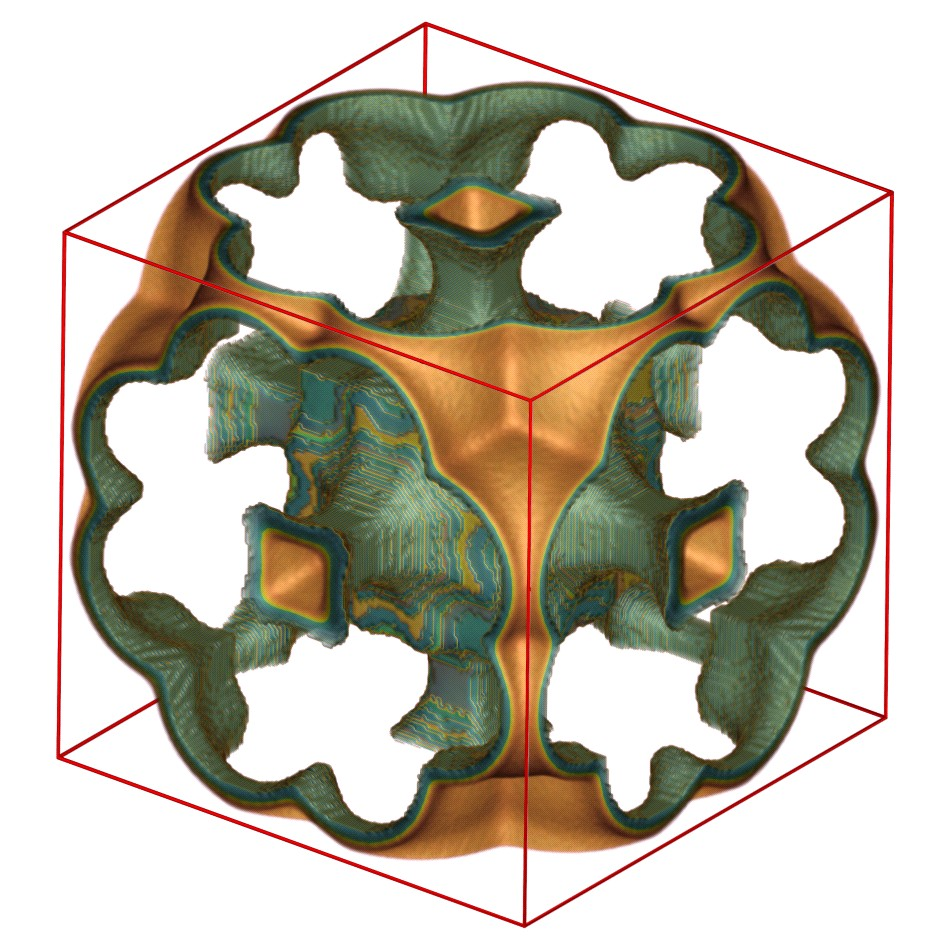
\includegraphics[width=4cm]{RHO.jpg}
\end{figure}}
\author{David Dubbeldam\footnote{email: d.dubbeldam@uva.nl}\\
Van 't Hoff Institute of Molecular Sciences, University of Amsterdam,\\
Science Park 904, 1098XH, Amsterdam, The Netherlands\\\\
Sofia Calero\footnote{email: scalero@upo.es}\\
Department of Physical, Chemical and Natural Systems,
University Pablo de Olavide,\\
Sevilla 41013, Spain\\\\
Donald E. Ellis\footnote{email: don-ellis@northwestern.edu}\\
Department of Physics and Astronomy, Northwestern University,\\
2145 Sheridan Road, Evanston IL  60208  USA\\\\
Randall Q. Snurr\footnote{email: snurr@northwestern.edu},\\
Chemical and Biological Engineering Department, Northwestern University,\\
2145 Sheridan Road, Evanston IL  60208,  USA}
\maketitle

\tableofcontents

\part{RASPA}
\chapter{Introduction}


\section{Design philosophy}

This software is a general purpose classical simulation package. It has been developed at
Northwestern University (Evanston, USA; group of Prof.\ Randall Q.\ Snurr) during 2006-2009 in active collaboration
with University Pablo de Olavide (Seville, Spain; group of Prof.\ Sofia Calero),
and from 2010-2015 also at the University of Amsterdam (David Dubbeldam) and 
Technical University of Delft (group of Prof.\ T.J.H.\ Vlugt).
It can be used for the simulation of molecules in gases, fluids, zeolites, aluminosilicates,
metal-organic frameworks, and carbon nanotubes.

Programs can be written in various ways, but often it is true that the fastest codes are probably the hardest to read,
while programs strictly based on readability lacks efficiency. RASPA is based on the following ideas:
\begin{itemize}
  \item{Correctness and accuracy}\\
  For all the techniques and algorithms available in RASPA we have implemented the 'best' ones available in literature. 
  For example, RASPA uses Configurational-Bias Monte-Carlo, it uses the Ewald summation for electrostatics,
  molecular dynamics is based on 'symplectic' integrators, all Monte-Carlo moves obey detailed balance etc.
  \item{Functional design}\\
  Looking at the source, you will notice that there are not a lot of files. The program is split up according to its function:
  'grid.c' contains the code to make and use a grid of a framework, 'ewald.c' handles all the electrostatic,'mc\_moves.c' contains all the
  moves to be used in Monte-Carlo,'potentials.c' contains all the VDW potentials etc.
  \item{Input made easy}\\
  The requirements for the input files is kept as minimal as possible. Only for more advanced options extra commands in the input file are
  needed. Also the format of the input is straightforward. Default settings are usually the best ones. Fugacity coefficients and excess
  adsorption are automatically computed.
  \item{Integrated simulation environment}\\
  The code is built up of many functions and routines which can be easily combined to do what you want. Molecular dynamics can be
  used in Monte Carlo and visa versa. Extension and modification of the code is relatively straightforward.
\end{itemize}

RASPA used three 'types' or 'groups' for the particles: 1) Framework atoms, 2) Adsorbates, and 3) Cations. The advantage is that
all the energies are split and the interactions can be examined (also the energies are split in the Ewald Fourier part).
Another example is when using thermostats in e.g. LTA5A where a different thermostat operates in the framework atoms, the adsorbates,
and the cations. These all move at different length- and time scales. Note that it is not possible to exchange types during
Identity-change moves (if defined they are ignored).


\section{Units and conventions}
\begin{itemize}
\item{The standard units in RASPA from which all other units are derived are:}\\
\vskip 0.1cm
\begin{tabularx}{\linewidth}{l|l|l|l}
 quantity & symbol & unit & value\\
\hline
 length      & $l$    & \AA ngstrom   & $10^{-10}$ m\\
 temperature & $T$    & Kelvin        & K\\
 mass        & $m$    & atomic mass   & $1.6605402\times 10^{-27}$ kg\\
 time        & $t$    & pico seconds  & $10^{-12}$ s\\
 charge      & $q$    & atomic charge & $1.60217733\times 10^{-19}$ C/particle\\
\hline
\end{tabularx}
\vskip 0.1cm

\noindent Some examples of derived units:\\

\begin{tabularx}{\linewidth}{l|l|l|l}
 quantity & symbol & units & conversion value\\
\hline
 energy             & $U$    & $J=\text{mass}\times\text{length}^2/\text{time}^2$ & $1.66054\times10^{-23}$ (=10 J/mol)\\
 pressure           & $p$    & $\text{Pa}=\text{mass}/(\text{length}\times\text{time}^2)$  & $1.66054\times10^7$\\
 diffusion constant & $D$    & $D=\text{length}^2/\text{time}$ & $1\times10^{-8}$\\
 force              & $f$    & $f=\text{length}/\text{time}^2$ & $1.66054\times 10^{-13}$\\
 \dots              & \dots  & \dots                                & \dots \\
\hline
\end{tabularx}\\

A pressure input of 10 Pascal in the input file, is converted to 'internal units' by dividing by $1.66054\times10^7$. In the
output any internal pressure is printed, multiplied by $1.66054\times10^7$. It is not necessary to convert units besides
input and output, with a few exceptions. One of them is the Coulombic conversion factor
\begin{equation}
  \frac{q_i q_j}{4\pi \epsilon_0}=\frac{\text{charge}^2}{4 \pi \times \text{electric constant}\times\text{length}\times\text{energy}}=138935.4834964017
\end{equation}
with the electric constant as $8.8541878176\times10^{-12}$ in units of $\text{C}^2/(\text{N}.\text{m}^2)$. This factor is needed to convert the
electrostatic energy to the internal units at every evaluation. 

\noindent
The Boltzmann's constant $k_B$ is
\begin{equation}
 k_B=\text{Boltzmann constant}/\text{energy}=0.8314464919
\end{equation}
with the Boltzmann constant as $1.380650324\times10^{-23}$ in units of J/K, and $k_B=0.8314464919$ in internal units.

\item{Numbering is based on the C-convention, i.e. starting from zero.}
\item{Files in the current directory always have preference.}\\
Sometimes one would like to try various parameters for force field fitting for example. In order to avoid
making a lot of directories for each force field it is more convenient to have the 
'pseudo\_atoms.def', 'force\_field\_mixing\_rule.def'
and 'force\_field.def' files in the \emph{current} directory.
\end{itemize}

\section{Compiling and installing RASPA}

\subsection{Requirements}

RASPA needs a C compiler, like 'gcc' or intel's 'icc' compilers, and optionally 
the libraries 'fftw', 'blas', and 'lapack'.

\subsection{RASPA from 'git'}

Working with 'git' and a remote repository  means that you will have to distinguish between two locations of the code:
\begin{enumerate}
 \item{The repository (visible to everyone)}
 \item{your local copy (only visible to you)}
\end{enumerate}

To check-out the code for the first time do:
\begin{verbatim}
     git clone https://github.com/iraspa/RASPA2
\end{verbatim}
After that, you can update the code by using
\begin{verbatim}
     git pull
\end{verbatim}

\subsection{installing RASPA}

The \emph{RASPA\_DIR} environment variable should be set to where you would like to install RASPA.
A common way of defining it is using the bash-shell
\begin{quote}
  export RASPA\_DIR=\$\{HOME\}/RASPA/simulations/
\end{quote}
or
\begin{quote}
  setenv RASPA\_DIR "\$\{HOME\}/RASPA/simulations/"
\end{quote}
for 'csh' and 'tcsh' shells.
It is possible to add this line to ".bashrc", "/etc/bashrc", "/etc/profile" etc, depending on the unix-version and
shell version to automatically have the environment variable set at login.

Note that the source-code of RASPA is kept separate from the installation data. RASPA needs the environment variable to
locate various files it needs, e.g. molecule definitions, framework definitions, force and field definitions.
It looks for these files relative to the RASPA\_DIR directory.

Before installing RASPA with
\begin{verbatim}
    make install
\end{verbatim}
from the top-directory, the code needs to be compiled.

\subsection{compiling RASPA}

RASPA uses the standard 'configure' utilities (autoconf, automake, libtool, and make).
The steps to install from scratch, i.e. after a 'make distclean' or 'git clone' are
\begin{enumerate}
 \item{\verb=rm -rf autom4te.cache=}
 \item{\verb=mkdir m4=}
 \item{\verb=aclocal=}
 \item{\verb=autoreconf -i=}
 \item{\verb=automake --add-missing=}
 \item{\verb=autoconf=}
 \item{\verb,./configure --prefix=${RASPA_DIR},  \qquad or\\
       \verb=./scripts/CompileScript/make-gcc-local=}
 \item{\verb=make=}
\end{enumerate}
where '\$\{RASPA\_DIR\}' is the directory you would like to install RASPA, and the commands
are executed in the top directory.

Usually (when recent automake and autoconf versions are installed), it is enough to do
\begin{enumerate}
  \item{\verb=make clean=}
  \item{\verb,./configure --prefix=${RASPA_DIR},}
  \item{\verb=make=}
\end{enumerate}

You can use the 'CFLAGS' environment variable to set compiler options and 'CC' to set the compiler.
For example, for a gcc compiler one could use
\begin{verbatim}
    export CFLAGS="-Wall -O3 -ffast-math"
    export CC="gcc"
\end{verbatim}

\subsection{Running RASPA\label{Introduction: running RASPA}}
Running RASPA is based on two files:
\begin{itemize}
 \item{A 'run' file to execute the program}\\
  an example file is:
  \begin{verbatim}
    #! /bin/sh -f
    export RASPA_DIR=${HOME}/Research/simulations/
    $RASPA_DIR/bin/simulate
  \end{verbatim}
  This type of file is know as a 'shell script'. RASPA needs the variable 'RASPA\_DIR' to be set in order
  to look up the molecules, frameworks, etc. The scripts sets the variable and runs RASPA. RASPA can then be run
  from any directory you would like.
 \item{An 'input'-file describing the type of simulation and the parameters}\\
  In the same directory as the 'run'-file, there needs to be a file called 'simulation.input'. An example file is:
  \begin{verbatim}
    SimulationType                   MonteCarlo
    NumberOfCycles                   100000
    NumberOfInitializationCycles     10000
    PrintEvery                       1000

    Box 0
    BoxLengths 30 30 30
    ExternalTemperature 300.0

    component 0 methane
                TranslationProbability           1.0
                CreateNumberOfMolecules          100
  \end{verbatim}
  This tells RASPA to run a Monte-Carlo simulation of 100 methane molecules in a $30\times30\times30$ \AA\ cubic box (with 90$^\circ$ angles)
  at 300 Kelvin. It will start with 10000 cycles to equilibrate the system and will use 100000 cycle to obtain thermodynamic properties
  of interest. Every 1000 cycles a status-report is printed to the output. The Monte-Carlo program will use only the 'translation move'
  where a particle is given a random translation and the move is accepted or rejected based on the energy difference.
  \end{itemize}


In order to run it on a cluster using a queuing system one needs an additional file 'bsub.job' (arbitrary name)
\begin{itemize}
 \item{'gridengine'}
  \begin{verbatim}
     #!/bin/csh
     # Serial sample script for Grid Engine
     # Replace items enclosed by {}
     #$ -S /bin/csh
     #$ -N Test
     #$ -V
     #$ -cwd
     echo $PBS_JOBID > jobid
     setenv RASPA_DIR ${HOME}/RASPA/simulations/
     $RASPA_DIR/bin/simulate
  \end{verbatim}
The job can be submitted using 'qsub bsub.job'.
 \item{'torque'}
  \begin{verbatim}
     #!/bin/bash
     #PBS -N Test
     #PBS -o pbs.out
     #PBS -e pbs.err
     #PBS -r n
     #PBS -V
     #PBS -mba
     cd $PBS_O_WORKDIR
     echo $PBS_JOBID > jobid
     export RASPA_DIR=${HOME}/RASPA/simulations
     ${RASPA_DIR}/bin/simulate
  \end{verbatim}
The job can be submitted using 'qsub bsub.job'.
 \item{'slurm'}
\begin{verbatim}
  #!/bin/bash 
  #SBATCH -N 1
  #SBATCH --job-name=Test
  #SBATCH --export=ALL
  echo $SLURM_JOBID > jobid
  valhost=$SLURM_JOB_NODELIST
  echo $valhost > hostname
  module load slurm
  ${RASPA_DIR}/bin/simulate
\end{verbatim}
The job can be submitted using 'sbatch bsub.job'.
\end{itemize}


\section{Output from RASPA}
RASPA generates output from the simulation. Some data is just information on the status, while other data are written because you
specifically asked the program to compute it for you. The output is written to be used with other programs like:
\begin{itemize}
 \item{gnuplot}
 \item{VTK}
 \item{iRASPA}
 \item{VMD}
\end{itemize}

The main output is written to the directory 'Output/System\_0/', 'Output/System\_1/', \dots for each of the simulated
systems. Usually one simulates only a single system. However, the Gibbs ensemble requires 2 systems, one for vapor phase and one
for the liquid phase, while $n$ systems are used by the (hyper-) parallel-tempering technique(s).

\section{Citing RASPA}

If you are using RASPA and would like to cite it in your journal articles or book-chapters, then for RASPA:

\begin{quote}
D. Dubbeldam, S. Calero, D.E. Ellis, and R.Q. Snurr,
\newblock RASPA: Molecular Simulation Software for Adsorption and Diffusion in Flexible Nanoporous Materials,
\newblock {\em Mol. Simulat.}, \url{http://dx.doi.org/10.1080/08927022.2015.1010082}, 2015.
\end{quote}
For the inner workings of Monte Carlo codes:
\begin{quote}
D. Dubbeldam, A. Torres-Knoop, and K.S. Walton,
\newblock On the Inner Workings of Monte Carlo Codes,
\newblock  \url{http://dx.doi.org/10.1080/08927022.2013.819102}
\newblock {\em Mol. Simulat.}, 39(14-15), 1253-1292, 2013.
\end{quote}
For the description of Molecular Dynamics and diffusion:
\begin{quote}
D. Dubbeldam and R.Q. Snurr,
\newblock Recent Developments in the Molecular Modeling of Diffusion in Nanoporous Materials,
\newblock  \url{http://dx.doi.org/10.1080/08927020601156418},
\newblock {\em Mol. Simulat.}, 33(4-5), 305-325, 2007.
\end{quote}
For the description of the implementation of force fields:
\begin{quote}
D. Dubbeldam, K.S. Walton, T.J.H. Vlugt, and S. Calero,
\newblock Design, Parameterization, and Implementation of Atomic Force Fields for Adsorption in Nanoporous Materials,
\newblock  \url{https://doi.org/10.1002/adts.201900135},
\newblock {\em Adv. Theory Simulat.}, 2(11), 1900135, 2019.
\end{quote}



\chapter{Format of the Input Files}

\section{Introduction}

In order to run a simulation you need several input-files:
\begin{itemize}
\item{\verb=`simulation.input'=}\\
This file contains the information on the type of simulation, the amount of steps, the framework name, number of unit cells
in each directions, the used molecules, the type of used Monte-Carlo moves etc.\
\item{\verb=`structure-name.cif'=}\\
If a framework (e.g.\ a zeolite or MOF) is used, then the definition of the structure needs to be provided. CIF-files are supported and the default input.
The name of the file should be equal to the one provided in \verb=`simulation.input'=, e.g.\ IRMOF-1.cif if \verb=`Frameworkname IRMOF-1'= is listed in
\verb=`simulation.input'=.
\item{\verb=`pseudo_atoms.def'=}\\
The \verb=`pseudo_atoms.def'= file list all the information on used pseudo-atoms, e.g.\ charge, mass. Usually a pseudo-atom is an atom, but there are exceptions
like united atoms (where CH3 is lumped into one unit) and off-atom sites in Tip5p water that represent oxygen lone pairs.
Because in CIF-files for frameworks you can provide also
information on atoms, there is no need to list framework atoms here if a CIF-file is used. On reading the CIF-file these defined atoms are added to the
pseudo-atoms. If also provided in the \verb=`pseudo_atoms.def'= then the definition in the \verb=`pseudo_atoms.def'= file has priority.
\item{\verb=`force_field_mxing_rules.def'=,\verb=`force_field.def'=}\\
The force field defined on the pseudo-atoms in \verb=`pseudo_atoms.def'=. These files list the Van der Waals potential types, the parameters, whether to
use tail-corrections, whether to shift to zero at the cutoff, and the type of mixing rule.
Force fields in literature are usually published in two forms: 1) a list of potentials parameters per atom and a mixing rule, or 2) pairs of atoms and parameters.
The first option corresponds to the file \verb=`force_field_mxing_rules.def'= and the latter option to the file \verb=`force_field.def'=. You can use both
at the same time, where \verb=`force_field.def'= has precedence over \verb=`force_field_mxing_rules.def'=.
\item{\verb=`molecule-name.def'=}\\
The definition of the used molecules.
The name of the file should be equal to the one provided in \verb=`simulation.input'=, e.g.\ propane.def if \verb=`MoleculeName propane'= is listed in
\verb=`simulation.input'=.
\item{\verb=zframework.def'=}\\
Used for a flexible framework to define all the bonds, bends, torsions, core-shells, etc.
\end{itemize}

The format of these files will be described in the remaining sections. Chapter \ref{Examples: chapter} provides lots of examples to see everything in action.
In addition to the input-files you will need either a \verb=`run'= file that is executable, or a queuing-script to submit the job to the queue
(see \ref{Introduction: running RASPA}).

\section{Simulation input}

Leading spaces and comments at the end of each line are omitted. Empty lines are skipped, 
and case is not important except in file names (i.e. framework and molecule names).

\subsection*{Simulation types}
\begin{itemize}
\item{SimulationType MonteCarlo}\\
Starts the Monte Carlo part of RASPA. The particular ensemble is not specified but implicitly deduced from
the specified Monte Carlo moves. Note that a MD-move can be used for hybrid MC/MD.
\item{SimulationType MolecularDynamics}\\
Starts the Molecular Dynamics part of RASPA. The ensemble is explicitly specified.
\item{SimulationType Spectra}\\
Starts the computation of the vibrational analysis. Possible options include infra red spectrum at zero Kelvin,
powder diffraction, and mode analysis.
\item{SimulationType Minimization}\\
Starts the minimization routine. It produces configurations and crystal structures at zero Kelvin.
\item{SimulationType Visualization}\\
Output VTK-files for snapshots and crystal structures, including energy surface pictures.
\item{SimulationType BarrierCrossing}\\
Routine for the dynamical correction of dynamically corrected Transition State Theory.
\item{SimulationType Numerical}\\
Computes all the forces numerically from the energy and compares them to the analytical expressions.
Also the strain-derivative tensor (related to the stress tensor), and the second derivative of
the energy with respect to strain, as well as the Hessian matrix can be checked.
\item{SimulationType MakeGrid}\\
Creates pre-tabulated energy-grids for use in rigid frameworks.
\end{itemize}

\subsection*{Simulation duration}
\begin{itemize}
\item{NumberOfCycles [int]}\\
The number of cycles for the production run. 
For Monte Carlo a cycle consists of $N$ steps, where $N$ is the amount of
molecules with a minimum of 20 steps. This means that on average during each cycle on each molecule a
Monte Carlo move has been attempted (either successful or unsuccessful). For MD the number of cycles
is simply the amount of integration steps.
\item{NumberOfInitializationCycles [int]}\\
The number of cycles used to initialize the system using Monte Carlo. This can be used for both Monte Carlo
as well as Molecular Dynamics to quickly equilibrate the positions of the atoms in the system.
\item{NumberOfEquilibrationCycles [int]}\\
For Molecular Dynamics  it is the number of MD steps to equilibrate the velocities in the systems. After this 
equilibration the production run is started. For Monte Carlo, in particular CFMC, the equilibration-phase is used
to measure the biasing factors.
\end{itemize}

\subsection*{Restart and crash-recovery}
\begin{itemize}
\item{RestartFile [yes$|$no]}\\
Reads the positions, velocities, and force from the directory `RestartInitial'. Any creation of molecules
in the `simulation.input' file will be in addition and after this first read from file. This is useful to
load initial positions of cations for example, and after that create adsorbates. The restart file
is written at `PrintEvery' intervals.
\item{ContinueAfterCrash [yes$|$no]}\\
Write a binary file containing the complete status of the program. 
The file name is `binary\_restart.dat' and is located in the directory `CrashRestart'.
With this option to `yes' the presence of this file will result in continuation from
the point where the program was at the moment of outputting this file.
The file can be quite big (several hundreds of megabytes) and will be outputted every
`WriteBinaryRestartFileEvery' cycles.
\item{WriteBinaryRestartFileEvery [int]}\\
The output frequency (i.e. every [int] cycles) of the crash-recovery file.
\end{itemize}

\subsection*{Printing options}
\begin{itemize}
\item{PrintEvery [int]}\\
Prints the loadings (when a framework is present) and energies every [int] cycles. For MD information
like energy conservation and stress are printed.
\item{PrintPropertiesEvery [int]}\\
Output running averages of many properties (i.e. Henry coefficients and elastic constants).
\item{PrintForcefieldToOutput [yes$|$no]}\\
Prints the force field information to the output-file.
Default: yes.
\item{PrintPseudoAtomsToOutput [yes$|$no]}\\
Prints the pseudo-atom information to the output-file.
Default: yes.
\item{PrintMoleculeDefinitionToOutput [yes$|$no]}\\
Prints the molecule definition information to the output-file.
Default: yes.
\end{itemize}

\subsection*{Force field definitions}
\begin{itemize}
\item{ChargeFromChargeEquilibration [yes$|$no]}\\
Compute the charges of the framework using the `charge-equilibration'-method.
\item{SymmetrizeFrameworkCharges [yes$|$no]}\\
All charges of the framework are made equivalent for equivalent framework atoms. 
Using regular charge-equilibration the charges are different for symmtrically equivalent
framework atoms, and this options restores the symmetry.
\item{ForceField [string]}\\
Reads in the force field [string], first the file `pseudo\_atoms.def' is read, then 
`force\_field\_mixing\_rules.def' and finally `force\_field.def'. The latter overwrites
general settings for interactions based on mixing rules with specific ones for individual
interactions. 

Note that if any of these files are in the working directory then these will read and used instead of the
ones in `\$\{RASPA\_DIR\}/simulations/share/raspa/forcefield/[string]'.

\item{CutOffVDW [real]}\\
The cutoff of the Van der Waals potentials. Interactions longer then this distance are omitted from the
energy and force computations. The potential can either be shifted to zero at the cutoff, or interactions
can just neglected after the cut off, or the remainder of the potential energy can be approximated using
tail corrections. This is specified in the force field files and can be specified globally or
for each interaction individually.
\item{CutOffVDWSwitch [real]}\\
The distance at which VDW switching will start. The smoothing will make sure the value and derivatives are zero at the cutoff.
The default: 0.9 times the CutOff.
\item{CutOffChargeCharge [real]}\\
The cutoff of the charge-charge potential. The potential is truncated at the cutoff and only shifted when `ChargeMethod CoulombShifted'
or `ChargeMethod CoulombSmoothed' is used.
No tail-corrections are (or can be) applied. The only way to include the long-range part is to use `ChargeMethod Ewald'.
The parameter is also used in combination with the
Ewald precision to compute the number of wave vectors and Ewald parameter $\alpha$.
For the Ewald summation using rather large unit cells, a charge-charge cutoff of about half the smallest box-length would be advisable
in order to avoid the use of an excessive amount of wave-vectors in Fourier space. For non-Ewald methods the cutoff should be as large
as possible (greater than about 30 \AA).
\item{CutOffChargeChargeSwitch [real]}\\
The distance at which charge-charge switching will start. The smoothing will make sure the value and derivatives are zero at the cutoff.
The default: 0.65 times the CutOff.
\item{CutOffChargeBondDipole [real]}\\
The cutoff of the charge-bonddipole potential.
\item{CutOffChargeBondDipoleSwitch [real]}\\
The distance at which charge-bonddipole switching will start. The smoothing will make sure the value and derivatives are zero at the cutoff.
The default: 0.70 times the CutOff.
\item{CutOffBondDipoleBondDipole [real]}\\
The cutoff of the bonddipole-bonddipole potential.
\item{CutOffBondDipoleBondDipoleSwitch [real]}\\
The distance at which bonddipole-bonddipole switching will start. The smoothing will make sure the value and derivatives are zero at the cutoff.
The default: 0.75 times the CutOff.


\item{OmitAdsorbateAdsorbateVDWInteractions [yes$|$no]}\\
Omits the Van der Waals interactions between adsorbates.
\item{OmitAdsorbateAdsorbateCoulombInteractions [yes$|$no]}\\
Omits the Coulombic (i.e. Ewald) interactions between adsorbates.
\item{OmitInterMolecularInteractions [yes$|$no]}\\
Omits the interactions between all molecules (only interactions with the framework). This also
works with the Ewald summation on. The options implies the setting of both
\begin{itemize}
  \item{OmitAdsorbateAdsorbateVDWInteractions [yes$|$no]}
  \item{OmitAdsorbateAdsorbateCoulombInteractions [yes$|$no]}
\end{itemize}
\item{InternalFrameworkLennardJonesInteractions [yes$|$no]}\\
Compute the Van der Waals interaction of the flexible framework. The Demontis flexible model for silicalite
is defined with only bond, bend, and torsion for example. One can use this option and also use
`Charge None'.
\item{$\begin{array}{l}\text{RemoveBondNeighboursFromLongRangeInteraction [yes$|$no]}\\
      \text{RemoveBendNeighboursFromLongRangeInteraction [yes$|$no]}\\
      \text{RemoveTorsionNeighboursFromLongRangeInteraction [yes$|$no]}\end{array}$}\\
After construction of the connectivity table all interactions are removed from Van der Waals and charge
interactions that are defined as 1-2 (i.e. bonds), 1-3 (i.e. bends, Urey-Bradley) and 1-4 (i.e. torsion, inversion-bend) respectively.
\item{Remove12NeighboursFromChargeChargeInteraction [yes$|$no]\\
      Remove13NeighboursFromChargeChargeInteraction [yes$|$no]\\
      Remove14NeighboursFromChargeChargeInteraction [yes$|$no]}\\
Remove all 1-2, 1-3, and/or 1-4 interactions within the framework from the long-range charge-charge
interaction within the flexible framework respectively.
\item{Remove12NeighboursFromChargeBondDipoleInteraction [yes$|$no]\\
      Remove13NeighboursFromChargeBondDipoleInteraction [yes$|$no]\\
      Remove14NeighboursFromChargeBondDipoleInteraction [yes$|$no]}\\
Remove all 1-2, 1-3, and/or 1-4 interactions within the framework from the long-range charge-bond dipole
interaction within the flexible framework respectively.
\item{Remove12NeighboursFromBondDipoleBondDipoleInteraction [yes$|$no]\\
      Remove13NeighboursFromBondDipoleBondDipoleInteraction [yes$|$no]\\
      Remove14NeighboursFromBondDipoleBondDipoleInteraction [yes$|$no]}\\
Remove all 1-2, 1-3, and/or 1-4 interactions within the framework from the long-range bond dipole-bond dipole
interaction within the flexible framework respectively.
\end{itemize}

\subsection*{Thermostat and barostat parameters}
\begin{itemize}
\item{ExternalTemperature [list-of-reals]}\\
The external temperature in Kelvin for each system. Because the system is in contact with this imaginary reservoir the
average temperature of the system can be controlled. Default: 298K.
\item{ExternalPressure [list-of-reals]}\\
The external pressure in Pascal for each system. Because the system is in contact with this imaginary reservoir the
average pressure of the system can be controlled. 
\item{ThermostatChainLength [int]}\\
The length of the chain to thermostat the system. Default: 5.
\item{BarostatChainLength [int]}\\
The length of the chain to thermostat the volume and/or cell parameters. Default 5.
\item{NumberOfYoshidaSuzukiSteps [int]}\\
The number of Yoshida/Suzuki multiple timesteps.
\item{TimeScaleParameterThermostat [real]}\\
The time scale on which the system thermostat evolves. Default: 0.15 ps.
\item{TimeScaleParameterBarostat [real]}\\
The time scale on which the thermostat for the volume and/or cell parameters evolve. Default: 0.15 ps.
\end{itemize}

\subsection*{Molecular dynamics parameters}
\begin{itemize}
\item{TimeStep [real]}\\
The time step in picoseconds for MD integration. Default value: 0.0005 ps (0.5 fs).
\item{Ensemble [list-of-{\scriptsize NVE$|$NVT$|$NPT$|$NPH$|$NPTPR$|$NPHPR}]}\\
Sets the ensemble as a list of NVE,NVT, NPT, NPH, NPTPR, or NPHPR for each system. If only a single ensemble is given, it is used for all systems.
The given ensemble will be used for both initialization as well as the production run.
\begin{itemize}
\item{NVE}\\
The micro canonical ensemble, the number of particle $N$, the volume $V$, and the energy $E$ are constant.
\item{NVT}\\
The canonical ensemble, the number of particle $N$, the volume $V$, and the average temperature $\left\langle P\right\rangle$
are constant. Instantaneous values for the temperature are fluctuating.
\item{NPT}\\
The isobaric-isothermal ensemble, the number of particle $N$, the average pressure $\left\langle P\right\rangle$, and the average temperature $\left\langle P\right\rangle$
are constant. Instantaneous values for the pressure and temperature are fluctuating.
\item{NPH}\\
The isoenthalpic-isobaric ensemble, the number of particle $N$, the average pressure $\left\langle P\right\rangle$, and the enthalpy $H$
are constant. Instantaneous values for the pressure and temperature are fluctuating.
\item{NPTPR}\\
The isobaric-isothermal ensemble with a fully flexible cell (Parrinello-Rahman).
\end{itemize}
\item{InitEnsemble [list-of-{\scriptsize NVE$|$NVT$|$NPT$|$NPH$|$NPTPR$|$NPHPR}]}\\
Sets the ensemble as a list of NVE,NVT, NPH, NPTPR, or NPHPR for each system. If only a single ensemble is given, it is used for all systems.
The given ensemble will be only used for the initialization run.
\item{RunEnsemble [list-of-{\scriptsize NVE$|$NVT$|$NPT$|$NPH$|$NPTPR$|$NPHPR}]}\\
Set the ensemble as a list of NVE,NVT, NPH, NPTPR, or NPHPR for each system. If only a single ensemble is given, it is used for all systems.
The given ensemble will be only used for the production run.
\item{NPTPRCellType [list-of-{\scriptsize Regular$|$Monoclinic$|$RegularUpperTriangle$|$MonoclinicUpperTriangle$|$Isotropic$|$Anisotropic}]}\\
The type of constraints on the cell-matrix $\mathbf{h}$. Default: RegularUpperTriangle.
\begin{itemize}
\item{Regular}\\
If the pressure tensor is asymmetric ($P_{\alpha\beta}\not=P_{\beta\alpha}$) at a given instant of
time, then there will be a net torque acting on the cell that will cause it to rotate. Cell
rotations can be eliminated by using the symmetrized tensor $P_{\alpha\beta}= (P_{\alpha\beta}+P_{\beta\alpha})/2$ in the
equations of motion and setting the initial total angular momentum of the cell to zero.
This approach is formally implemented by constraining the force on the cell $\mathbf{g}=\mathbf{g}^T$.
All three angles $\alpha,\beta,\gamma$ are allowed to change, as well as the box lengths $\mathbf{a},\mathbf{b},\mathbf{c}$.
\item{Monoclinic}\\
All three box lengths $\mathbf{a},\mathbf{b},\mathbf{c}$ are allowed to vary, as well as cell angle $\beta$, but $\alpha=\gamma=90^\circ$.
\item{RegularUpperTriangle}\\
Only the upper triangular part of the cell matrix is used to eliminate rotation of the box.
All three angles $\alpha,\beta,\gamma$ are allowed to change, as well as the box lengths $\mathbf{a},\mathbf{b},\mathbf{c}$.
\item{MonoclinicUpperTriangle}\\
Only the upper triangular part of the cell matrix is used to eliminate rotation of the box.
All three box lengths $\mathbf{a},\mathbf{b},\mathbf{c}$ are allowed to vary, as well as cell angle $\beta$, but $\alpha=\gamma=90^\circ$.
\item{Isotropic}\\
All three box lengths $\mathbf{a}=\mathbf{b}=\mathbf{c}$ are allowed to vary isotropically, and the angles remain fixed $\alpha=\beta=\gamma=90^\circ$.
\item{Anisotropic}\\
All three box lengths $\mathbf{a},\mathbf{b},\mathbf{c}$ are allowed to vary \emph{independently}, but the angles remain fixed $\alpha=\beta=\gamma=90^\circ$.
\end{itemize}

\end{itemize}

\subsection*{Box parameters}
\begin{itemize}
\item{$\begin{array}{l}\text{Box [int]}\\ \text{[real] [real] [real]}\end{array}$}\\
Set the system [int] to type `Box' (other option is `Framework' when a framework is present).
The cell dimensions of rectangular box of system [int] in Angstroms. Default: 25 25 25 \AA.
\item{$\begin{array}{l}\text{BoxAngles [int]}\\ \text{[real] [real] [real]}\end{array}$}\\
Set the system [int] to type `Box' (other option is `Framework' when a framework is present).
The cell angles of rectangular box of system [int] in Angstroms. Default: 90$^\circ$ 90$^\circ$ 90$^\circ$.
\item{$\begin{array}{l}\text{BoxMatrix [int]}\\ 
      \text{[real] [real] [real]}\\
      \text{[real] [real] [real]}\\
      \text{[real] [real] [real]}\end{array}$\\
       }\\
Set the system [int] to type `Box' (other option is `Framework' when a framework is present).
The $3\times3$ cell matrix of system [int], given as three vectors (as columns). 
This is the most general form and any box can be specified in this way. Units of the vectors are Angstrom.
\end{itemize}


\subsection*{Framework parameters}
\begin{itemize}
\item{Framework [int]}\\
Set the system [int] to type `Framework' (other option is `Box' when no framework is present).
All other options listed in the section framework parameters refer to this system, so make sure this is before any other framework options.
\item{FrameworkName [string]}\\
Loads the framework with name [string]. Several frameworks can be read per system, 
which is useful for to study interpenetration of frameworks. Here the frameworks
are allowed to move independently from each other.
\item{HeliumVoidFraction [real]}\\
The void fraction as measure by probing the structure with helium a room temperature. This quantity has to be obtained from a separate
simulation and is essential to compute the \emph{excess}-adsorption during the simulation.
\item{UnitCells [int] [int] [int]}\\
The number of unit cells in x,y, and z direction for the system. The full cell will contain the unit cells, and periodic boundary conditions
will be applied on the box level (\emph{not} on a unit cell level).
\item{ShiftUnitCells [real] [real] [real]}\\
Shift the fractional positions so that the center of a framework can be altered.
\item{FlexibleFramework [yes$|$no]}\\
Allow the current framework of the current system to be fully flexible. The name of the flexible model is provided using the
`FrameworkDefinitions [string]' input option.
\item{FrameworkDefinitions [string]}\\
The force field name [string] of the flexible framework. The file is read even when `FlexibleFramework no' is specified (the reason is that 
framework bond-dipoles are defined using the `framework.def' file).
\item{ModifyFrameworkAtomConnectedTo [atom-type-1] [atom-type-2] [atom-type-3] [atom-type-4]}\\
Modifies the atom-type-1 to atom-type-2, always if atom-type-3 and atom-type-4 are omitted, or only it is connected to atom-type-3 when atom-type-3 is specified,
or only when it is connected to both atom-type-3 and atom-type-4 if both are specified.
\item{ModifyFrameworkDimer [atom-type-1] [atom-type-2] [atom-type-3] [atom-type-4]}\\
Modifies the connected atom-type-1 and atom-type-2 dimer to atom-type-3 and atom-type-4.
\item{ModifyFrameworkTriple [atom-type-1] [atom-type-2] [atom-type-3] [atom-type-4] [atom-type-5] [atom-type-6]}\\
Modifies the connected triple atom-type-1,atom-type-2,atom-type-3 to atom-type-4,atom-type-5,atom-type-6.
\item{RemoveAtomNumberCodeFromLabel [yes$|$no]}\\
Reading structure-files: the number is removed from the framework atom-types, e.g.\ \verb=`O1'=, \verb=`O2'=, \verb=`O3'=, etc.\ are mapped to \verb=`O'=.
\item{AddAtomNumberCodeToLabel [yes$|$no]}\\
Writing structure-files: the number is added to the framework atom-types, e.g.\ \verb=`O'= are mapped to \verb=`O1'=, \verb=`O2'=, \verb=`O3'=, etc.
\item{RestrictFrameworkAtomsToBox [yes$|$no]}\\
Restricts (places back) atoms to the unit cell dimensions, i.e. fractional positions between 0 and 1.
\item{ReadCIFAsCartesian [yes$|$no]}\\
Reads the position listed in the CIF-file as Cartesian. Only applicable to P1 systems (no symmetry).
\end{itemize}

\subsection*{System moves}

\begin{itemize}
\item{FrameworkChangeMoveProbability [real]}\\
The probability per cycle to randomly translate a framework atom. During this move the number of inner cycles is the amount of framework atoms, with a maximum of 500.
This move is applicable to relatively rigid structures like zeolites. For other structure where movement is caused by collective behavior (for example, the rotation of a phenyl-ring
in a metal-organic framework) the MC/MD move is more convenient. Such movement is hardly sampled at all by individual MC translation moves.
\item{VolumeChangeProbability [real]}\\
The probability per cycle to attempt a volume-change. Rigid molecules are scaled by center-of-mass, while flexible molecules and the framework is atomically scaled.
\item{BoxShapeChangeProbability [real]}\\
The probability per cycle to attempt a shape-change of the box. One of the 6 upper triangular elements of the box matrix is randomly chosen.
Rigid molecules are scaled by center-of-mass, while flexible molecules and the framework is atomically scaled.
\item{GibbVolumeChangeProbability [real]}\\
The probability per cycle to attempt a Gibbs volume-change MC move during a Gibbs ensemble simulation. The total volume of the two boxes 
(usually one for the gas phase, one for the liquid phase) remains constant, but the individual volume of the boxes are changed.
The volumes are changed by a random change in $\ln(V_I/V_{II})$.
\item{HybridNVEMoveProbability [real]}\\
The probability per cycle to attempt a hybrid Monte Carlo move using Molecular Dynamics in the NVE-ensemble.
The whole system is integrated using Newton's equations of motion. The new configuration
is then accepted or rejected using the standard MC rule. Note that the difference in energy $\Delta U$ is the integration error. The integration time step is set using
`TimeStep'.
\item{NumberOfHybridNVESteps [int]}\\
The number of integration steps for the hybrid MC/MD NVE move. Default: 5.
\item{ParallelTemperingProbability [real]}\\
A move where two neighboring systems 
are swapped that differ in their temperature.
\item{HyperParallelTemperingProbability [real]}\\
A move where two neighboring systems 
are swapped that differ in their temperature
and chemical potentials.
\item{ParallelMolFractionProbability [real]}\\
A move where two neighboring systems (similar to parallel tempering)
are swapped that differ in their mol-fraction of components $A$ and $B$.
\item{ParallelMolFractionComponentA [int]}\\
The identifier of the first component.
\item{ParallelMolFractionComponentB [int]}\\
The identifier of the second component.
\item{ChiralInversionProbability [real]}\\
A move specifically designed for systems with chiral molecules
to change all $S$-molecules into $R$-molecules and vica versa.
Note that the spacegroup needs to be set. If you have a framework that is P1 but has higher symmetry then use \verb=`CalculateSpaceGroup yes'= to
determine the true space group of the framework. An error will be given if this move is impossible for your system (e.g.\ when the framework is chiral).
\end{itemize}

\subsection*{Component information}
\begin{itemize}
\item{Component [int] MoleculeName [string]}\\
Reads in the definition of component [int] using the file `\emph{molecule-name-string}.def' from the 
directory `\$\{RASPA\_DIR\}/share/raspa/molecules/\emph{molecule-definitions-string}'.
\item{MoleculeDefinitions [string]}\\
The type of the molecule. For example, there could an OPLS version of the molecule, or a TraPPE version, etc. This \emph{molecule-definitions-string} is actually the directory name
under which the molecule file is found in `\$\{RASPA\_DIR\}/share/raspa/molecules/'.
\item{StartingBead [int]}\\
The staring bead for the configurational bias Monte Carlo (CBMC). In CBMC the molecule is grown bead by bead biasing the growth towards energetically favorable configurations.
Certain operations, like the rotation MC move and Widom particle insertion, use this bead as the center of rotation and position of the probe molecule, respectively.
\item{BlockPockets [yes$|$no]}\\
Block certain pockets in the simulation volume. The growth of a molecule is not allowed in a blocked pocket. A typical example is the sodalite cages in FAU and LTA-type zeolites,
these are not accessible to molecules like methane and bigger.
\item{BlockPocketsFileName [string]}\\
The file name for the definitions of all the blocking spheres.
\item{MolFraction [real]}\\
The mol fraction of this component in the mixture. The values can be specified relative to other components, as the fractions are normalized afterwards.
The partial pressures for each component are computed from the total pressure and the mol fraction per component.
\item{FugacityCoefficient [real]}\\
The fugacity coefficient for the current component. For values 0 (or by not specifying this line), the fugacity coefficients are automatically computed using the Peng-Robinson
equation of state. Note the critical pressure, critical temperature, and acentric factor need to be specified in the molecule file.
\item{Intra14VDWScalingValue [real]}\\
The scaling factor for intra-molecular 1-4 van der Waals interactions. For example: OPLS uses a factor of $\frac{1}{2}$.
\item{Intra14ChargeChargeScalingValue [real]}\\
The scaling factor for intra-molecular 1-4 charge/charge interactions. For example: OPLS uses a factor of $\frac{1}{2}$.
\item{IdealGasRosenbluthWeight [real]}\\
The ideal Rosenbluth weight is the growth factor of the CBMC algorithm for a single chain in an empty box. The value only depends on temperature and therefore needs to be computed
only once. For adsorption, specifying the value in advance is convenient because the applied pressure does not need to be corrected afterwards (the Rosenbluth weight corresponds to a shift
in the chemical potential reference value, and the chemical potential is directly obtained from the fugacity). For equimolar mixtures this is essential.
\item{GibbsSwapProbability [real]}\\
The relative probability to attempt a Gibbs swap MC move for the current component. The `GibbsSwapMove' transfers a randomly selected particle from one box to the other
(50\% probability to transfer a particle from box I to II, an 50\% visa versa).
\item{TranslationProbability [real]}\\
The relative probability to attempt a translation move for the current component. A random displacement is chosen in the allowed directions (see `TranslationDirection').
Note that the internal configuration of the molecule is unchanged by this move. The maximum displacement is scaled during the simulation to achieve an acceptance
ratio of 50\%.
\item{TranslationDirection 
      \begin{small}
       [X$|$Y$|$Z$|$XY$|$XZ$|$YZ$|$XYZ$|$A$|$B$|$C$|$AB$|$AC$|$BC$|$ABC$|$\\
      \hspace*{2cm}ORTHOGONAL\_TO\_AB\_DIR$|$ORTHOGONAL\_TO\_AC\_DIR$|$ORTHOGONAL\_TO\_BC\_DIR$|$\\
      \hspace*{2cm}ORTHOGONAL\_TO\_O\_AB\_DIR$|$ORTHOGONAL\_TO\_O\_AC\_DIR$|$ORTHOGONAL\_TO\_O\_BC\_DIR$|$\\
      \hspace*{2cm}ORTHOGONAL\_TO\_A\_BC\_DIR$|$ORTHOGONAL\_TO\_B\_AC\_DIR$|$ORTHOGONAL\_TO\_C\_AB\_DIR$|$\\
      \hspace*{2cm}ORTHOGONAL\_TO\_O\_ABC\_DIR]
     \end{small}}\\
Specifies the allowed translation direction for the current component. Useful to sampling configuration with the starting bead restricted to a plane, i.e. see dcTST.
Default: XYZ.
\item{RandomTranslationProbability [real]}\\
The relative probability to attempt a random translation move for the current component. The displacement is chosen such that any position in the box can reached. It is therefore
similar as reinsertion, but `reinsertion' changes the internal conformation of a molecule and uses biasing.
\item{RotationProbability [real]}\\ 
The relative probability to attempt a random rotation move for the current component. The rotation is around the starting bead. A random vector on a sphere
is generated, and the rotation is random around this vector.
\item{CBMCProbability [real]}\\
The relative probability to attempt a partial reinsertion move for the current component. Part of the molecule is regrown, while part of the molecule can remain fixed.
The list of partial reinsertion moves is specified in the `molecule.def' file.
\item{ReinsertionProbability [real]}\\
The relative probability to attempt a full reinsertion move for the current component. Multiple first beads are chosen, and one of these is selected according to its Boltzmann weight.
The remaining part of the molecule is grown using biasing. This move is very useful, and often necessary, to change the internal configuration of flexible molecules.
\item{SwapProbability [real]}\\
The relative probability to attempt a insertion or deletion move. Whether to insert or delete is decided randomly with a probability of 50\% for each.
The swap move imposes a chemical equilibrium between the system and an imaginary particle reservoir for the current component. The move starts with multiple first bead, and
grows the remainder of the molecule using biasing.
\item{WidomProbability [real]}\\
The relative probability to attempt a Widom particle insertion move for the current component. The Widom particle insertion moves measure the chemical potential
and can be directly related to Henry coefficients and heats of adsorption.
\item{SurfaceAreaProbability [real]}\\
The relative probability to attempt a surface-area move for the current component.
\item{ReinsertionInPlaceProbability [real]}\\
The relative probability to attempt a reinsertion-in-place move for the current component. The reinsertion position is the current position of the starting bead of the randomly selected
molecule. Alternatively, one can use the partial reinsertion move leaving one bead fixed. The move is very useful to sample configuration on a plane for dcTST to change
the internal configuration, e.g. bonds, bends, torsions, etc.
\item{IdentityChangeProbability [real]}\\
The relative probability to attempt an identity-change move for the current component. A molecule of type $A$ is reinsertion, in the same place as the starting bead of $A$, as type $B$ using
the starting bead of component $B$. The $A-B$ list is defined using `IdentityChangesList' defining $B$ for each component $A$, i.e. the current component can be reinserted into
any component defined in the `IdentityChangesList' list, and from that list the component is chosen randomly.
\item{NumberOfIdentityChanges [int]}\\
The number of `IdentityChangesList' elements for the current component.
\item{IdentityChangesList [list-of-int]}\\
The list of components that the current component can be changed into. The identity-change move will randomly choose the new component from this list.
\item{GibbsIdentityChangeProbability [real]}\\
The relative probability to attempt an identity change for the current component in the Gibbs ensemble.
It is a very useful move to for mixture of $n$ components. Out of the $n$ components, two components $i\not=j$ are selected at random.
At random, it is selected to switch the identity of component $i$
in box $I$ or in box $II$, and the identity of the component $j$ in the other box.
In each box, a particle is selected at random which matches the desired identity.
\item{NumberOfGibbsIdentityChanges [int]}\\
The number of `GibbsIdentityChangesList' elements for the current component.
\item{GibbsIdentityChangesList [list-of-int]}\\
The list of components that the current component can be changed into. The Gibbs-identity-change move will randomly choose the new component from this list.
\item{ExtraFrameworkMolecule [yes$|$no]}\\
There are two major types of molecules, `Adsorbates' and `Cations'. The `ExtraFrameworkMolecule' keyword sets whether the current component is a `Cation' (yes) or a `Adsorbate' (no).
Energies in the output as splitted in Host-Host, Host-Adsorbate, Host-Cation, Adsorbate-Adsorbate, Cation-Cation, and Adsorbate-Cation. The distinction in two types of molecule
is sometimes necessary. For example, consider a mixture of components, where polarization needs to be neglected between certain components (because they are parameterized without).
The water model `rpol' is defined including polarization, but CO2 using TraPPE is not. One can define water as `Adsorbate', CO2 as `Cation' and neglect polarization between cations.
\item{RestrictEnantionface [yes$|$no]}\\
Restricts all MC-moves to the enantioface defined by `Enantioface'. Moves that result in an opposite enantioface are rejected.
\item{Enantioface [Re$|$Si]}\\
The enantioface of the component, either `Re' or `Si'.
\item{EnantiofaceAtoms \begin{footnotesize}[F$|$A$|$C] [int] [int] [F$|$A$|$C] [int] [int] [F$|$A$|$C] [int] [int]
 [F$|$A$|$C] [int] [int] [F$|$A$|$C] [int] [int]\end{footnotesize}}\\
The definition of the enantioface based on 5 atoms. The first 4 form a torsion, as well as the first 3 and the last atom. These two torsions form the definition
of the enantioface.
\item{CreateNumberOfMolecules [int]}\\
The number of molecule to create for the current component. Note these molecules are \emph{in addition} to anything read in by using a restart-file. Usually, when the restart-file
is used the amount here should be put back to zero. A warning, putting this value unreasonably high results in an infinite loop. The routine accepts molecules that are grown causing
no overlap (energy smaller than `EnergyOverlapCriteria'). Also the initial starting configurations are far from optimal and substantial equilibration is needed to reduce the energy.
However, the CBMC growth is able to reach very high densities.
\end{itemize}


\subsection*{Options to measure properties}
\begin{itemize}

\item{ComputeDistanceHistograms [yes$|$no]}\\
Sets whether or not to compute the histograms of specified distance pairs for the current system.
A directory `DistanceHistograms' is created containing the histograms for each system.
\begin{itemize}
\item{WriteDistanceHistogramEvery [int]}\\
Output the distance histograms every [int] cycles.
\item{MaxRangeDistanceHistogram [real]}\\
The range of the histograms.
\item{NumberOfElementsDistanceHistogram [int]}\\
The number of elements of the histograms.
\item{DistanceHistogramDefinition [F$|$A$|$C] [int] [int] [F$|$A$|$C] [int] [int]}\\
Define a distance histogram between two atoms.
\end{itemize}

\item{ComputeBendAngleHistograms [yes$|$no]}\\
Sets whether or not to compute the bend-angle histograms of specified trimers of atoms for the current system.
A directory `BendAngleHistograms' is created containing the histograms for each system.
\begin{itemize}
\item{WriteBendAngleHistogramEvery [int]}\\
Output the distance histograms every [int] cycles.
\item{MaxRangeBendAngleHistogram [real]}\\
\item{NumberOfElementsBendAngleHistogram [int]}\\
\item{BendAngleHistogramDefinition [F$|$A$|$C] [int] [int] [F$|$A$|$C] [int] [int] [F$|$A$|$C] [int] [int]}\\
\end{itemize}

\item{ComputeDihedralAngleHistograms [yes$|$no]}\\
Sets whether or not to compute the dihedral-angle histograms of specified quads of atoms for the current system.
A directory `DihedralAngleHistograms' is created containing the histograms for each system.
\begin{itemize}
\item{WriteDihedralAngleHistogramEvery [int]}\\
Output the distance histograms every [int] cycles.
\item{MaxRangeDihedralAngleHistogram [real]}\\
\item{NumberOfElementsDihedralAngleHistogram [int]}\\
\item{DihedralAngleHistogramDefinition \small{[F$|$A$|$C] [int] [int] [F$|$A$|$C] [int] [int] [F$|$A$|$C] [int] [int] [F$|$A$|$C] [int] [int]}}\\
\end{itemize}

\item{ComputeAngleBetweenPlanesHistograms [yes$|$no]}\\
Sets whether or not to compute the histograms of angles between specified planes for the current system.
A directory `AngleBetweenPlanesHistograms' is created containing the histograms for each system.
\begin{itemize}
\item{WriteAngleBetweenPlanesHistogramEvery [int]}\\
Output the distance histograms every [int] cycles.
\item{MaxRangeAngleBetweenPlanesHistogram [real]}\\
\item{NumberOfElementsAngleBetweenPlanesHistogram [int]}\\
\item{AngleBetweenPlanesHistogramDefinition [F$|$A$|$C] [int] [int] [F$|$A$|$C] [int] [int] [F$|$A$|$C] [int] [int]
        [F$|$A$|$C] [int] [int] [F$|$A$|$C] [int] [int] [F$|$A$|$C] [int] [int]}\\
\end{itemize}


\item{ComputePSD [yes$|$no]}\\
Sets whether or not to compute the pore-size distribution (PSD) for the current system.
A directory `PoreSizeDistributionHistogram' is created containing the output 
`HistogramPoreSizeDistribution.dat' per system.
\begin{itemize}
\item{WritePSDEvery [int]}\\
Output the PSD every [int] cycles.
\item{PSDProbeDistance [Minimum$|$Sigma]}\\
Sets whether to use the minimum of the potential $\sigma^{1/6}$ as the probe distance or whether to use $\sigma$.
\item{HistogramSizePoreSizeDistribution [int]}\\
default: 100.
\item{MaxRangePoreSizeDistribution [real]}\\
default: 10.
\end{itemize}


\item{ComputeRDF [yes$|$no]}\\
Sets whether or not to compute the radial distribution function (RDF) for the current system.
A directory `RadialDistributionFunctions' is created containing the output per system.
The RDF is computed for each atom type pair unless the option `print' flag in `pseudo\_atoms.def'
is `no'.
\begin{itemize}
\item{WriteRDFEvery [int]}\\
Output the RDF every [int] cycles.
\end{itemize}

\item{ComputeMSD [yes$|$no]}\\
Sets whether or not to compute the mean-squared displacement (MSD) for the current system using a modified order-N algorithm.
A directory `MSDOrderN' is created containing the output per system. The output consists of files containing self-msd data per
component, the total self-msd, the Onsager msd for each component pair, and the the total Onsager msd.
The units in the files are \AA$^2$ for the msd, and ps for time.
  \begin{itemize}
    \item{WriteMSDEvery [int]}\\
     Output the MSD every [int] cycles.
    \item{SampleMSDEvery [int]}\\
    Samples every [int] integration steps. Default: 1.
    \item{ComputeIndividualMSD [yes$|$no]}\\
    Computes the msd, not only per component, but also per molecule.
    \item{NumberOfBlocksMSD [int]}\\
    The  number of blocks for the order-$n$ correlation measurement. Each block represent a different time-scale of sampling. Default: 25.
    \item{NumberOfBlockElementsMSD [int]}\\
    The number of elements in each block. For example, if the number is 10, then the first block samples: $1,2,3,\dots,10$, the second block
    $10,20,30,\dots,100$, the third block $100,200,300,\dots,1000$, etc. Default: 25.
   \end{itemize}

\item{ComputeVACF [yes$|$no]}\\
Sets whether or not to compute the velocity autocorrelation function (VACF) for the current system using a modified order-N algorithm.
A directory `VACFOrderN' is created containing the output per system. The output consists of files containing self-vacf data per
component, the total self-vacf, the Onsager vacf for each component pair, and the the total Onsager vacf.
The files start with the integration diffusivity-values, computed using a generalization of the Simpson's rule 
(in the sense that it is exact for cubic polynomials and is valid for an odd as well as even number of intervals).
The units in the files are \AA$^2$/ps for velocity, and ps for time.
  \begin{itemize}
    \item{WriteVACFEvery [int]}\\
     Output the VACF every [int] cycles.
    \item{SampleVACFEvery [int]}\\
    Samples every [int] integration steps. Default: 5.
    \item{ComputeIndividualVACF [yes$|$no]}\\
    Computes the vacf, not only per component, but also per molecule.
    \item{NumberOfBlocksVACF [int]}\\
    The  number of blocks for the order-$n$ correlation measurement. Each block represent a different time-scale of sampling. Default: 10.
    \item{NumberOfBlockElementsVACF [int]}\\
    The number of elements in each block. For example, if the number is 10, then the first block samples: $1,2,3,\dots,10$, the second block
    $10,20,30,\dots,100$, the third block $100,200,300,\dots,1000$, etc. Default: 5000.
   \end{itemize}

\item{ComputeRVACF [yes$|$no]}\\
Sets whether or not to compute the rotational velocity autocorrelation function 
(RVACF) for the current system using a modified order-N algorithm.
A directory `RVACFOrderN' is created containing the output per system. The output consists of files containing self-rvacf data per
component, the total self-rvacf, the Onsager rvacf for each component pair, and the the total Onsager rvacf.
The files start with the integration diffusivity-values, computed using a generalization of the Simpson's rule
(in the sense that it is exact for cubic polynomials and is valid for an odd as well as even number of intervals).
The units in the files are \AA$^2$/ps for velocity, and ps for time.
  \begin{itemize}
    \item{WriteRVACFEvery [int]}\\
     Output the RVACF every [int] cycles.
    \item{SampleRVACFEvery [int]}\\
    Samples every [int] integration steps. Default: 5.
    \item{ComputeIndividualRVACF [yes$|$no]}\\
    Computes the vacf, not only per component, but also per molecule.
    \item{NumberOfBlocksRVACF [int]}\\
    The  number of blocks for the order-$n$ correlation measurement. Each block represent a different time-scale of sampling. Default: 10.
    \item{NumberOfBlockElementsRVACF [int]}\\
    The number of elements in each block. For example, if the number is 10, then the first block samples: $1,2,3,\dots,10$, the second block
    $10,20,30,\dots,100$, the third block $100,200,300,\dots,1000$, etc. Default: 5000.
   \end{itemize}

\item{ComputeMOACF [yes$|$no]}\\
Sets whether or not to compute the molecular orientation velocity autocorrelation function
(MOACF) for the current system using a modified order-N algorithm.
A directory `MOACFOrderN' is created containing the output per system. The output consists of files containing self-moacf data per
component and the total self-rvacf.
The units in the files are rad$^2$/ps for velocity, and ps for time.
  \begin{itemize}
    \item{WriteMOACFEvery [int]}\\
     Output the MOACF every [int] cycles.
    \item{SampleMOACFEvery [int]}\\
    Samples every [int] integration steps. Default: 5.
    \item{ComputeIndividualMOACF [yes$|$no]}\\
    Computes the moacf, not only per component, but also per molecule.
    \item{NumberOfBlocksMOACF [int]}\\
    The  number of blocks for the order-$n$ correlation measurement. Each block represent a different time-scale of sampling. Default: 10.
    \item{NumberOfBlockElementsMOACF [int]}\\
    The number of elements in each block. For example, if the number is 10, then the first block samples: $1,2,3,\dots,10$, the second block
    $10,20,30,\dots,100$, the third block $100,200,300,\dots,1000$, etc. Default: 5000.
   \end{itemize}


\item{ComputeMSDConventional [yes$|$no]}\\
Sets whether or not to compute the mean-squared displacement (MSD) for the current system using the conventional algorithm.
A directory `MSD' is created containing the output per system. The routine is available for legacy reasons,
the same results can be obtained using the order-N method and 1 block of size `BufferLengthMSD'.
The units in the files are \AA$^2$ for the msd, and ps for time.
  \begin{itemize}
    \item{WriteMSDConventionalEvery [int]}\\
     Output the MSD every [int] cycles. Default: 5000.
    \item{SampleMSDConventionalEvery [int]}\\
    Samples every [int] integration steps. Default: 1.
    \item{NumberOfBuffersMSDConventional [int]}\\
    The number of (overlapping) buffers with a different offset in time. Default: 20.
    \item{BufferLengthMSDConventional [int]}\\
    The length of the buffers. Default: 5000.
   \end{itemize}


\item{ComputeVACFConventional [yes$|$no]}\\
Sets whether or not to compute the velocity autocorrelation function (VACF) for the current system using the conventional algorithm.
A directory `VACF' is created containing the output per system. The routine is available for legacy reasons, 
the same results can be obtained using the order-N method and 1 block of size `BufferLengthVACF'.
The units in the files are \AA$^2$/ps for velocity, and ps for time.
  \begin{itemize}
    \item{WriteVACFConventionalEvery [int]}\\
     Output the VACF every [int] cycles. Default: 5000.
    \item{SampleVACFConventionalEvery [int]}\\
    Samples every [int] integration steps. Default: 1.
    \item{NumberOfBuffersVACFConventional [int]}\\
    The number of (overlapping) buffers with a different offset in time. Default: 20.
    \item{BufferLengthVACFConventional [int]}\\
    The length of the buffers. Default: 5000.
   \end{itemize}

\item{ComputeDensityHistograms [yes$|$no]}\\
Sets whether or not to compute a density histogram for the current system. For example, during adsorption it keeps track of the amount of molecules.

\item{ComputeEnergyHistogram [yes$|$no]}\\
Sets whether or not to compute a histogram of the energy for the current system. 
For example, during adsorption it keeps track of the total energy, the VDW energy,
the Coulombic energy, and the polarization energy. Output is written to  the directory
`EnergyHistograms'.
\begin{itemize}
\item{WriteEnergyHistogramEvery [int]}\\
Sets to print the energy histogram of the system every [int] cycles.
\item{EnergyHistogramSize [int]}\\
Sets the number of elements of the histogram. Default: 1000.
\item{EnergyHistogramLowerLimit [real]}\\
Sets the lower limit of the histogram. Default: -10000.
\item{EnergyHistogramUpperLimit [real]}\\
Sets the upper limit of the histogram. Default: 0.
\end{itemize}

\item{ComputeThermoDynamicFactor [yes$|$no]}\\
Sets whether or not to compute the thermodynamic factors of the energy for the current system. 
The output is written to the directory `ThermoDynamicFactor'.
\begin{itemize}
\item{WriteThermoDynamicFactorEvery [int]}\\
Sets to print the thermodynamic factors every [int] cycles.
\end{itemize}

\item{ComputeEndToEndDistanceHistograms [yes$|$no]}\\
Sets whether or not to compute a histogram for end-to-end distances of molecules for the current system.

\item{ComputePrincipleMomentsOfInertia [yes$|$no]}\\
Sets whether or not to compute the average principle moments of inertia of molecules for the current system.

\item{ComputeSpectra [yes$|$no]}\\
Sets whether or not to compute the Infra-Red (IR) spectra of molecules for the current system.
\begin{itemize}
\item{WriteSpectraEvery [int]}\\
Sets to print the spectra of molecules every [int] cycles.
\end{itemize}
\item{ComputeMoleculeProperties [yes$|$no]}\\
Sets whether or not to compute properties of molecules like average bond-lengths, average bend-angles etc. for the current system.
\item{PrintMoleculePropertiesEvery [int]}\\
Sets to print the properties of molecules every [int] cycles.
\item{ComputeSurfaceArea [yes$|$no]}\\
Sets whether or not to compute the surface.
\begin{itemize}
\item{SurfaceAreaProbeAtom [string]}\\
\item{SurfaceAreaSamplingPointsPerSphere [int]}\\
Sets the number of points to sampling a sphere per iteration.
\item{SurfaceAreaProbeDistance [Minimum$|$Sigma]}\\
Sets whether to use the minimum of the potential $\sigma^{1/6}$ as the probe distance or whether to use $\sigma$.
\end{itemize}
\item{DensityProfile [yes$|$no]}\\
\item{DensityProfileGridPoints [int] [int] [int]}\\
\item{ComputeElasticConstants [yes$|$no]}\\
Sets whether to compute elastic constants.
\item{ComputePowderDiffractionPattern [yes$|$no]}\\
Sets whether to compute the powder diffraction pattern for the framework.
\begin{itemize}
\item{DiffractionType [Xray$|$Neutron$|$Electron]}\\
Sets the diffraction type as xray-scattering, neutron-scattering, or electron-scattering, respectively.
\item{DiffractionRadiationType [chromium$|$iron$|$copper$|$molybdenum$|$silver$|$synchrotron]}\\
Sets the type of the diffraction radiation as chromium, iron, copper, molybdenum, silver, or synchrotron, respectively.
\item{WaveLengthType [Single$|$Double]}\\
Set the type of the beam as single or as a doublet.
\item{PeakShape [Gaussian$|$Lorentzian$|$PseudoVoigt]}\\
Sets the shape of the peaks as Gaussian, Lorentzian, or Pseudo-Voigt, respectively.
\item{WaveLength [real]}\\
Sets the wavelength of the diffraction beam.
\item{TwoThetaMin [real]}\\
Sets the minimum value of $2\theta$.
\item{TwoThetaMax [real]}\\
Sets the maximum value of $2\theta$.
\item{TwoThetaStep [real]}\\
Sets the step size of $2\theta$.
\item{PeakWidthModifierU [real]}\\
\item{PeakWidthModifierV [real]}\\
\item{PeakWidthModifierW [real]}\\
\end{itemize}
\item{ComputerNormalModes [yes$|$no]}\\
Sets whether to compute normal modes.
\begin{itemize}
\item{MinimumMode [int]}\\
Sets the minimum normal to compute.
\item{MaximumMode [int]}\\
Sets the maximum normal to compute.
\item{ModeResolution [int]}\\
\end{itemize}
\end{itemize}

\subsection*{Energy/force grid options}
\begin{itemize}
\item{UseTabularGrid [yes$|$no]}\\
Use a pre-tabulated grid for the energy and forces. Default: no.
\item{SpacingVDWGrid [real]}\\
The grid spacing of the Van der Waals potentials. Default: 0.15 Angstrom.
\item{SpacingCoulombGrid [real]}\\
The grid spacing of the Coulomb potential. Default: 0.15 Angstrom.
\item{GridTypes [list-of-strings]}\\
A list of atom-types for each of the used grids.
\end{itemize}

\subsection*{Minimization/Saddle point search}
\begin{itemize}
\item{MinimizationMethod [Baker]}\\
The Baker minimization method uses the eigenvalues/vectors to find a true minimum where all eigenvalues are positive. Newton-Raphson
uses the first and second derivatives, but not the eigenvalues/vectors.
The saddle point search can best be started from a minimum energy configuration. The algorithm walks up hill along the softest eigen mode
to find a first order saddle point.
\item{MinimizationVariables [Cartesian$|$Fractional]}\\
Whether the minimization is performed in Cartesian or fractional positions. For some crystal minimizations it might be more convenient
to choose fractional positions. An example is when one wants to keep a particular fractional position fixed during the minimization.
\item{MaximumNumberOfMinimizationSteps [int]}\\
The maximum number of minimization steps after which the minimization is stopped. Default: 10000.
\item{RMSGradientTolerance [real]}\\
Stopping criteria: the maximum allowed RMS gradient. Default: $10^{-6}$.
\item{MaxGradientTolerance [real]}\\
Stopping criteria: the maximum allowed gradient for each and every atom (and the strain elements for cell minimizations). Default: $10^{-6}$.
\item{MaximumStepLength [real]}\\
The maximum length of a minimization step. The length is dependent on the problem at hand.
A too low value converges slowly (i.e. the minimization takes more steps),
while a too high value might not converge at all. Default value: 0.3.
\item{FrameworkFixedInitialization [free$|$fixed]}\\
Sets all framework atoms as `free' or `fixed'. This command must preceed individual overwrites
and applies to the current system.
\item{AdsorbateFixedInitialization [free$|$fixed]}\\
Sets all adsorbate groups and atoms as `free' or `fixed'. This command must preceed individual overwrites
and applies to the current system.
\item{CationFixedInitialization [free$|$fixed]}\\
Sets all cation groups and atoms as `free' or `fixed'. This command must preceed individual overwrites
and applies to the current system.
\item{ActiveFrameworkAtom [int]}\\
Sets the atom of the current framework and system as `active'.
\item{ActiveFrameworkAtoms [int] [list-of-ints]}\\
Sets the [int] atoms listed in [list-of-ints] of the current framework and system as `active'.
\item{FixedFrameworkAtom [int]}\\
Sets the atom of the current framework and system as `fixed'.
\item{FixedFrameworkAtoms [int] [list-of-ints]}\\
Sets the [int] atoms listed in [list-of-ints] of the current framework and system as `fixed'.

\item{ActiveAdsorbateMolecule [int]}\\
Sets all atom and groups of the adsorbate molecule [int] as `active'. Applies to the current system.
\item{FixedAdsorbateMolecule [int]}\\
Sets all atom and groups of the adsorbate molecule [int] as `fixed'. Applies to the current system.
\item{ActiveAdsorbateAtom [int] [int]}\\
Sets an atom (second argument) of an adsorbate molecule (first argument) as `active'. Applies to the current system.
\item{FixedAdsorbateAtom [int] [int]}\\
Sets an atom (second argument) of an adsorbate molecule (first argument) as `fixed'. Applies to the current system.
\item{ActiveAdsorbateGroup [int] [int]}\\
Sets a group (second argument) of an adsorbate molecule (first argument) as `active'. Applies to the current system
and both center of mass and the orientation are set as `active'.
\item{FixedAdsorbateGroup [int] [int]}\\
Sets a group (second argument) of an adsorbate molecule (first argument) as `fixed'. Applies to the current system
and both center of mass and the orientation are set as`fixed'.
\item{ActiveAdsorbateGroupCenterOfMass [int] [int]}\\
Sets a group (second argument) of an adsorbate molecule (first argument) as `active'. Applies to the current system
and only the center of mass is set as `active'.
\item{FixedAdsorbateGroupCenterOfMass [int] [int]}\\
Sets a group (second argument) of an adsorbate molecule (first argument) as `fixed'. Applies to the current system
and only the center of mass is set as `fixed'.
\item{ActiveAdsorbateGroupOrientation [int] [int]}\\
Sets a group (second argument) of an adsorbate molecule (first argument) as `active'. Applies to the current system
and only the orientation is set as `active'.
\item{FixedAdsorbateGroupOrientation [int] [int]}\\
Sets a group (second argument) of an adsorbate molecule (first argument) as `fixed'. Applies to the current system
and only the orientation is set as `fixed'.

\item{ActiveCationMolecule [int]}\\
Sets all atom and groups of the cation molecule [int] as `active'. Applies to the current system.
\item{FixedCationMolecule [int]}\\
Sets all atom and groups of the cation molecule [int] as `fixed'. Applies to the current system.
\item{ActiveCationAtom [int] [int]}\\
Sets an atom (second argument) of an cation molecule (first argument) as `active'. Applies to the current system.
\item{FixedCationAtom [int] [int]}\\
Sets an atom (second argument) of an cation molecule (first argument) as `fixed'. Applies to the current system.
\item{ActiveCationGroup [int] [int]}\\
Sets a group (second argument) of an cation molecule (first argument) as `active'. Applies to the current system
and both center of mass and the orientation are set as `active'.
\item{FixedCationGroup [int] [int]}\\
Sets a group (second argument) of an cation molecule (first argument) as `fixed'. Applies to the current system
and both center of mass and the orientation are set as `fixed'.
\item{ActiveCationGroupCenterOfMass [int] [int]}\\
Sets a group (second argument) of an cation molecule (first argument) as `active'. Applies to the current system
and only the center of mass is set as `active'.
\item{FixedCationGroupCenterOfMass [int] [int]}\\
Sets a group (second argument) of an cation molecule (first argument) as `fixed'. Applies to the current system
and only the center of mass is set as `fixed'.
\item{ActiveCationGroupOrientation [int] [int]}\\
Sets a group (second argument) of an cation molecule (first argument) as `active'. Applies to the current system
and only the orientation is set as `active'.
\item{FixedCationGroupOrientation [int] [int]}\\
Sets a group (second argument) of an cation molecule (first argument) as `fixed'. Applies to the current system
and only the orientation is set as `fixed'.




\item{$\begin{array}{l}\text{FixAtomType [string]}\\\text{FixAtomTypes [int] [list-of-strings]}\end{array}$}\\
The atom-types that are considered fixed during the minimization. All other atoms/groups will be optimized.
If the atom-type is contained in a rigid unit, the entire unit will be frozen.
\item{DistanceConstraint [F$|$A$|$C] [int] [int] [F$|$A$|$C] [int] [int] [real]}\\
Defines a `hard' distance constraint between two atoms and/or groups, and the distance.
\item{AngleConstraint [F$|$A$|$C] [int] [int] [F$|$A$|$C] [int] [int] [F$|$A$|$C] [int] [int] [real]}\\
Defines a `hard' angular constraint between three atoms and/or groups, and the constraint angle.
\item{DihedralConstraint [F$|$A$|$C] [int] [int] [F$|$A$|$C] [int] [int]
    [F$|$A$|$C] [int] [int] [F$|$A$|$C] [int] [int] [real]}\\
Defines a `hard' dihedral constraint between four atoms and/or groups, and constraint dihedral.
\item{HarmonicDistanceConstraint [F$|$A$|$C] [int] [int] [F$|$A$|$C] [int] [int] [real] [real]}\\
Defines a `hard' distance constraint between two atoms and/or groups, and the distance.
\item{HarmonicAngleConstraint \begin{small}[F$|$A$|$C] [int] [int] [F$|$A$|$C] [int] [int] 
  [F$|$A$|$C] [int] [int]  [real] [real]\end{small}}\\
Defines a `hard' angular constraint between three atoms and/or groups, and the constraint angle.
\item{HarmonicDihedralConstraint \begin{footnotesize}[F$|$A$|$C] [int] [int] [F$|$A$|$C] [int] [int]
 [F$|$A$|$C] [int] [int] [F$|$A$|$C] [int] [int] [real] [real]\end{footnotesize}}\\
Defines a `hard' dihedral constraint between four atoms and/or groups, and constraint dihedral.
\end{itemize}

\subsection*{Monte Carlo settings}
\begin{itemize}
\item{MinimumInnerCycles [int]}\\
The minimum number of inner cycles for each cycle. Default: 20.
\item{NumberOfTrialPositions [int]}\\
The number of trial positions during the growth of a molecule. Default: 10.
\item{NumberOfTrialPositionsForTheFirstBead [int]}\\
The number of trial positions for the first bead. Default: 10.
\item{NumberOfTrialPositionsTorsion [int]}\\
The number of trial positions for torsions over a single bond. Default: 100.
\item{NumberOfTrialMovesPerOpenBead [int]}\\
The number of trial moves per open bead during CBMC. Default: 200.
\item{TargetAccRatioSmallMCScheme [real]}\\
\item{TargetAccRatioTranslation [real]}\\
\item{EnergyOverlapCriteria [real]}\\
The energy criteria to consider an energy as `overlap'. Default: $10^5$ K.
\item{MinimumRosenbluthFactor [real]}\\
The minimum Rosenbluth weight, values lower are consider to be `overlapping'. Default: $10^{-150}$.
\end{itemize}

\subsection*{Biasing options}
\begin{itemize}
\item{BiasingDirection [A$|$B$|$C$|$AB\_DIAGONAL$|$AC\_DIAGONAL$|$BC\_DIAGONAL$|$\\
              \hspace*{2.65cm} A\_BC\_DIAGONAL$|$B\_AC\_DIAGONAL$|$C\_AB\_DIAGONAL$|$\\
              \hspace*{2.65cm} O\_ABC\_DIAGONAL]}\\
\item{BiasingMethod [UMBRELLA$|$RUIZMONTERO]}\\
\item{BiasingProfile [string]}\\
The name of the file containing the biasing profile.
\item{RuizMonteroFactor [real]}
\item{UmbrellaFactor [real]}\\
The biasing free energy is multiplied by the UmbrellaFactor. This is useful when the biasing free energy goes to infity in certain regions. if the
exact free energy would be used to biased, then the histogram would be flat, even very close to atoms. To keep the repulsion one can lower the used free
energy biasing by e.g.\ multiplying by 0.9.
\item{RestrictMovesToUnitCell [yes$|$no]}\\
Restrict the Monte-Carlo moves to the first unitcell for this component.
\item{BoxAxisABC\_Min [real]}\\
When a particle is restricted in all Monte-Carlo moves (RestrictMovesToUnitCell or RestrictMovesToBox) then do not allow trial moves with a fractional position smaller than BoxAxisABC\_Min.
\item{BoxAxisABC\_Max [real]}\\
When a particle is restricted in all Monte-Carlo moves (RestrictMovesToUnitCell or RestrictMovesToBox) then do not allow trial moves with a fractional position greater than BoxAxisABC\_Max.
\end{itemize}

\subsection*{Transition State Theory settings}
\begin{itemize}
\item{\begin{minipage}{\textwidth}
      FreeEnergyMappingType  [A\_MAPPING$|$B\_MAPPING$|$C\_MAPPING$|$ABC\_MAPPING$|$\\
        \hspace*{4cm}MAP\_AB\_DIAGONAL$|$MAP\_AC\_DIAGONAL$|$MAP\_BC\_DIAGONAL$|$\\
        \hspace*{4cm}MAP\_A\_BC\_DIAGONAL$|$MAP\_B\_AC\_DIAGONAL$|$MAP\_C\_AB\_DIAGONAL$|$\\
        \hspace*{4cm}MAP\_O\_ABC\_DIAGONAL]
      \end{minipage}
      }
Determines how the free energy profile is constructed from the contributions of points in the unit cell.
The free energy is computed using Widom insertion by inserting probe molecules
at many random position inside the unit cell. The `FreeEnergyMappingType' maps a Cartesian position on a reaction coordinate `q'.
The mappings `A\_MAPPING', `B\_MAPPING', `C\_MAPPING' map the Cartesian position onto the `a', `b', `c' lattice vectors.
The diagonal mapping maps onto diagonal, either in 2D or in 3D. For example, `MAP\_A\_BC\_DIAGONAL' maps onto the line from `A' to `B+C' where
`A',`B', and `C' are the end points of the lattive vectors; and `MAP\_O\_ABC\_DIAGONAL' maps onto the line from the origin to the opposite point `A+B+C' on the diagonal.
\item{\begin{minipage}{\textwidth}
      PositionHistogramMappingType  [A\_MAPPING$|$B\_MAPPING$|$C\_MAPPING$|$ABC\_MAPPING$|$\\
        \hspace*{4cm}MAP\_AB\_DIAGONAL$|$MAP\_AC\_DIAGONAL$|$MAP\_BC\_DIAGONAL$|$\\
        \hspace*{4cm}MAP\_A\_BC\_DIAGONAL$|$MAP\_B\_AC\_DIAGONAL$|$MAP\_C\_AB\_DIAGONAL$|$\\
        \hspace*{4cm}MAP\_O\_ABC\_DIAGONAL]
      \end{minipage}
      }
Determines how the position histogram is constructed from the contributions of points in the unit cell.
The free energy is computed from the histogram by using $F(q)=-\log\left[P\left(q\right)\right]$.
The `PositionHistogramMappingType' maps a Cartesian position on a reaction coordinate `q'.
The mappings `A\_MAPPING', `B\_MAPPING', `C\_MAPPING' map the Cartesian position onto the `a', `b', `c' lattice vectors.
The diagonal mapping maps onto diagonal, either in 2D or in 3D. For example, `MAP\_A\_BC\_DIAGONAL' maps onto the line from `A' to `B+C' where
`A',`B', and `C' are the end points of the lattive vectors; and `MAP\_O\_ABC\_DIAGONAL' maps onto the line from the origin to the opposite point `A+B+C' on the diagonal.
\item{PutMoleculeOnBarrier [yes$|$no]}\\
Places the first molecule of component 0 at the position given by `BarrierPosition'. This is used e.g. to start sampling configuration on top of a free energy barrier.
\item{BarrierPosition [real] [real] [real]}\\
The location of the free energy barrier in fractional units of the first unit cell.
\item{MaxBarrierDistance [real]}\\
The maximum distance in \AA ngstrom of the dcTST trajectory.
\item{MaxBarrierTime [real]}\\
The maximum time of the dcTST trajetory in picoseconds.
\item{NumberOfVelocities [int]}\\
The number of times the same initial position of the sampled dcTST starting configurations is used with different initial velocities.
\item{WritedcTSTSnapShotsToFile [yes$|$no]}\\
Whether to write out sampled configuration to a file. The file is stored in the directory `dcTST\_starting\_configurations' and used
as the tarting point to compute the transmission coefficient in dcTST.
\item{WritedcTSTSnapShotsEvery [int]}\\
The frequency in MC cycles of writing out the sampled configurations. Default: 1000.
\end{itemize}

\section{Force field}

\subsection{Force fields}

\subsection{`pseudo\_atoms.def'}

The `pseudo\_atoms.def' files describes the (pseudo-)atoms to be used in the simulation. An example is
is the definitions for the tip5p water model:
\begin{scriptsize}
\begin{verbatim}
  #number of pseudo atoms
  3
  #type  print as  scat  oxidation mass       charge  polarization B-factor radii connectivity anisotropic anisotropic-type   tinker-type
  Ow     yes    O     O          0 15.9994    0.0     0.0          1.0      0.5   2            0.0         absolute           0
  Hw     yes    H     H          0 1.0008     0.241   0.0          1.0      1.00  1            0.0         absolute           0
  L      yes    L     -          0 0.0       -0.241   0.0          1.0      1.00  1            0.0         absolute           0
\end{verbatim}
\end{scriptsize}
The first line is skipped, the second line is the number of (pseudo-)atoms, the third line is skipped again, and next
all the (pseudo-)atoms are specified. The format and meaning is:

\begin{tabularx}{\linewidth}{|>{\columncolor{light-blue}}c|>{\columncolor{niceyellow2}}X|}
\doublerulesepcolor{red}
\arrayrulecolor{red}
\hline
 name & An unique string of character to be used to identify the atom. The same name has be used in other files to refer
        to this atom.\\
 \hline
 print & Whether or not this atom should be printed to movies. The dummy `L' atoms of the tip5p water model are an example
         where you would like them to be skipped, only the `O' and `H' atoms should be printed.\\
 \hline
 as    & The string to be printed to movies.\\
 \hline
 scat  & The chemical symbol, e.g. O, O$^{-}$, O$^{2-}$. They are defined in `scattering\_factors.c' and are used only in powder diffraction
         and spectra.\\
 \hline
 oxidation & not used yet\\
 \hline
 mass  & The mass of the atom in atomic units.\\
 \hline
 charge & The charge of the atom in atomic units.\\
 \hline
 polarization & not used yet\\
 \hline
 B-factor & The temperature factor of the atom, used only in powder diffraction.\\
 \hline
 radius & The radius of the atom to be used to decide what atoms are considered as `neighbors'. The current rule is that
          two atoms $i$ and $j$ are considered `bonded' if the distance between the atoms is smaller then 0.56+Radius$_i$+Radius$_j$.\\
 \hline
 connectivity & The connectivity of the atoms (not yet used).\\
 \hline
 anisotropic factor & The magntitude of the anisotropy.\\
 \hline
 anisotropic-type   & The type of anisotropy, either `relative' or `absolute'. For example, 
                    a relative anisotropic factor of hydrogen of -0.077, used in the MM3 force field, 
                      means the site is pulled inward by 7.7\% (and located at 92.3\% of the C-H bondlength).
                      An absolute anisotropic factor of e.g. 0.3 means the site is displaced outward by 0.3\AA.\\
\hline
 Tinker-type        & The type of the atom in other codes, e.g. Tinker. This is used for output-files in formats used in other codes.\\
\hline
\doublerulesepcolor{white}
\end{tabularx}

\subsection{`force\_field\_mixing\_rules.def'}
\begin{verbatim}
        # general rule for shifted vs truncated
        shifted
        # general rule tailcorrections
        no
        # number of defined interactions
        9
        # type interaction
        Zn1            lennard-jones    0.42      2.7
        O1             lennard-jones    700.0     2.98
        O2             lennard-jones    70.5      3.11
        C1             lennard-jones    48.5      3.76
        C2             lennard-jones    47.86     3.47
        C3             lennard-jones    47.86     3.47
        H1             lennard-jones    7.65      2.85
        O_co2          lennard-jones    80.507    3.033
        C_co2          lennard-jones    28.129    2.757
        # general mixing rule for Lennard-Jones
        Jorgensen
\end{verbatim}
The first line is skipped, the second line is the general cutoff rule for shifted vs truncated, the third line is skipped, 
the fourth line is the general tule for tail corrections, the fifth line is skipped, the sixth line is the number of
defined self-interactions for the (pseudo-) atoms. The next line is skipped again followed by the defined potentials
for the (pseudo-)atoms. The file is ended with a skipped line and the general rule for the mixing rule. Note all these
interactions can be subsequently overwritten using the `force\_field.def' file for specific interactions.

For convenience, you can use pattern matching of the interactions. Any string $s_1$ ending with an underscore will match 
any string $s_2$ that starts with the substring $s_1$. Note that usually the `*' symbol is used, but this symbol has already a different
meaning for CIF-files. Of course patterns can match more than one atom, e.g. \verb=`C_'= matches \verb=`C1'= (a carbon atom) but also 
\verb=`Cl'= (chloride), and the rules are applied top to bottom. Therefore, list the generic ones first and the more specific after the generic patterns.

Example of a generic UFF/TraPPE force field for united atom alkanes in MOFs:
\begin{verbatim}
# general rule for shifted vs truncated
shifted
# general rule tailcorrections
no
# number of defined interactions
32
# type interaction, parameters.    IMPORTANT: define generic matches first
O_             lennard-jones    48.1581   3.03315
N_             lennard-jones    38.9492   3.26256
C_             lennard-jones    47.8562   3.47299
F_             lennard-jones    36.4834   3.0932
B_             lennard-jones    47.8058   3.58141
Cl_            lennard-jones   142.562    3.51932
Br_            lennard-jones   186.191    3.51905
H_             lennard-jones     7.64893  2.84642
Zn_            lennard-jones    62.3992   2.46155
Be_            lennard-jones    42.7736   2.44552
Cr_            lennard-jones     7.54829  2.69319
Fe_            lennard-jones     6.54185  2.5943
Mn_            lennard-jones     6.54185  2.63795
Cu_            lennard-jones     2.5161   3.11369
Co_            lennard-jones     7.04507  2.55866
Ga_            lennard-jones   208.836    3.90481
Ti_            lennard-jones     8.55473  2.8286
Sc_            lennard-jones     9.56117  2.93551
V_             lennard-jones     8.05151  2.80099
Ni_            lennard-jones     7.54829  2.52481
Zr_            lennard-jones    34.7221   2.78317
Mg_            lennard-jones    55.8574   2.69141
Ne_            lennard-jones    21.1352   2.88918
Ag_            lennard-jones    18.1159   2.80455
In_            lennard-jones   301.428    3.97608
Cd_            lennard-jones   114.734    2.53728
Sb_            lennard-jones   225.946    3.93777
Te_            lennard-jones   200.281    3.98232
He             lennard-jones    10.9      2.64
CH4_sp3        lennard-jones    158.5     3.72
CH3_sp3        lennard-jones    108.0     3.76
CH2_sp3        lennard-jones    56.0      3.96
# general mixing rule for Lennard-Jones
Lorentz-Berthelot
\end{verbatim}

Here, \verb=`CH4_sp3'=, \verb=`CH3_sp3'=, and \verb=`CH4_sp3'= are first matched by \verb=`C_'= but later overwritten with the correct values.
However, carbon atoms listed in the MOF CIF-file, like \verb=`C1'=, \verb=`C2'=,\verb=`C3'=, etc.\ will be set to the \verb=`C_'= value as intended.

\begin{tabularx}{\linewidth}{|>{\columncolor{light-blue}}X|>{\columncolor{niceyellow2}}X|>{\columncolor{niceyellow2}}X|}
\doublerulesepcolor{red}
\arrayrulecolor{red}
\hline
 general cutoff rule & `shifted' or `truncated' & `shifted' shifts the potentials to zero at the cutoff radius,
                       `truncated' leaves them unchanged.\\
\hline
 general tail corrections rule & `yes' or `no' & `yes' applies the tail corrections to all interactions,
                                                `no' omits the tail corrections for all interactions\\
\hline
 general mixing-rule (only used for Lennard-Jones) & `Jorgensen' or `Lorentz-Berthelot' & 
                             `Jorgensen' $\left\{\epsilon_{ij}=\sqrt{\epsilon_i \epsilon_j},
                                                  \sigma_{ij}=\sqrt{\sigma_i\sigma_j}\right\}$
                            `Lorentz-Berthelot' $\left\{\epsilon_{ij}=\sqrt{\epsilon_i \epsilon_j},
                                                        \sigma_{ij}=\frac{1}{2}\left(\sigma_i+\sigma_j\right)\right\}$\\
\hline
 self interaction type & `zero-potential',`12-6',`Lennard-Jones', `Buckingham', `MCY', `generic', `HIW',
                    `MIE', `BHM', or `Hydrogen' & the type of the potential determines the subsequent parameters, i.e.
                                                  Lennard-Jones expects a strength parameter $\epsilon_{ii}$ and a size
                                                  parameter $\sigma_{ii}$.\\
\hline
\doublerulesepcolor{white}
\end{tabularx}


\subsection{`force\_field.def'}

The `force\_field\_mixing\_rules.def' file given above can be used for the flexible model of the metal-organic
framework IRMOF-1. It is defined using the Jorgensen mixing rule and uses shifted potentials cutoff at 12 \AA.
The EMP2-CO$_2$ model however uses the Lorentz-Berthelot for CO$_2$-CO$_2$ interactions and uses a truncated
potential with tail corrections. Moreover, if we also want to use the DREIDING model for the CO$_2$-framework
interactions the correction-file `force\_field.def' would look like:

\begin{verbatim}
        # rules to overwrite
        3
        # pair      truncated/shifted tailcorrections
        O_co2 O_co2 truncated         yes
        O_co2 C_co2 truncated         yes
        C_co2 C_co2 truncated         yes
        # number of defined interactions
        14
        # type      type2       interaction    
        Zn1         C_co2       lennard-jones  27.34776042 3.420
        Zn1         O_co2       lennard-jones  46.77926891 3.545
        O1          C_co2       lennard-jones  36.07117963 2.915
        O1          O_co2       lennard-jones  61.70097244 3.04
        O2          C_co2       lennard-jones  36.07117963 2.915
        O2          O_co2       lennard-jones  61.70097244 3.04
        C1          C_co2       lennard-jones  35.94746166 3.135
        C1          O_co2       lennard-jones  61.48934867 3.26
        C2          C_co2       lennard-jones  35.94746166 3.135
        C2          O_co2       lennard-jones  61.48934867 3.26
        C3          C_co2       lennard-jones  35.94746166 3.135
        C3          O_co2       lennard-jones  61.48934867 3.26
        H1          C_co2       lennard-jones] 14.37184748 2.825
        H1          O_co2       lennard-jones] 24.58353107 2.95
        # mixing rules to overwrite
        1
        #
        O_co2 C_co2 Lorentz-Berthelot
\end{verbatim}

\begin{center}
\shadowbox{Tip: always double check the complete interaction set printed in the output !}
\end{center}

\section{Molecules}

The format of the molecules is designed to allow for a combination of flexible and rigid subunits. 
A molecule is made up of `groups', where a group
is a collection of either rigid or flexible atoms.

\subsection{Rigid molecule}

An example of CO$_2$ as a rigid molecule.
\begin{tiny}
\begin{verbatim}
        # critical constants: Temperature [T], Pressure [Pa], and Acentric factor [-]
        304.1282
        7377300.0
        0.22394
        #Number Of Atoms
        3
        # Number of groups
        1
        # CO2-group
        3
        rigid
        0 O_co2     0.0           0.0           1.16
        1 C_co2     0.0           0.0           0.0
        2 O_co2     0.0           0.0          -1.16
        # Chiral centers Bond  BondDipoles Bend  UrayBradley InvBend  Torsion Imp. Torsion Bond/Bond Stretch/Bend Bend/Bend Stretch/Torsion Bend/Torsion IntraVDW IntraCoulomb
                       0    2            0    0            0       0        0            0         0            0         0               0            0        0            0
        # Bond stretch: atom n1-n2, type, parameters
        0 1 RIGID_BOND
        1 2 RIGID_BOND
        # Number of config moves
        0
\end{verbatim}
\end{tiny}
The first three numbers are the critical constants: the critical temperature, the critical pressure, and the acentric factor.
They are used to automatically compute the fugacity from the pressure using an equation of state, e.g. Peng Robinson.
Then the number of atoms and the number of groups. The groups are listed one by one with first the number of atoms in the group,
whether it is rigid or flexible, and the atoms as number, type, and for a rigid molecule the relative positions.
After the groups follows the bond, bend, torsion etc. parameters. The file is ended with the config moves.
\subsection{Flexible molecule}
An example of a flexible molecule is the united-atom 2-methylbutane molecule. Note that for flexible units there
is not need to list relative positions. Bond-potentials are listed as the two atoms on which the potential operates,
the potential type and the corresponding parameters. At the end we have 2 config moves defined, one where atoms 0,1,2
are kept fixed and the rest is regrown, and another config move where only atoms 2,3 are kept fixed.
\begin{tiny}
\begin{verbatim}
        # critical constants: Temperature [T], Pressure [Pa], and Acentric factor [-]
        460.35
        3395700.0
        0.2296
        # Number Of Atoms
        5
        # Number Of Groups
        1
        # Alkane-group
        5
        flexible
        0 CH3_sp3
        1 CH_sp3
        2 CH2_sp3
        3 CH3_sp3
        4 CH3_sp3
        # Chiral centers Bond  BondDipoles Bend  UrayBradley InvBend  Torsion Imp. Torsion Bond/Bond Stretch/Bend Bend/Bend Stretch/Torsion Bend/Torsion IntraVDW IntraCoulomb
                       0    4            0    4            0       0        2            0         0            0         0               0            0        0            0
        # Bond stretch: atom n1-n2, type, parameters
        0 1 HARMONIC_BOND 96500 1.54
        1 2 HARMONIC_BOND 96500 1.54
        1 4 HARMONIC_BOND 96500 1.54
        2 3 HARMONIC_BOND 96500 1.54
        # Bond bending: atom n1-n2-n3, type, parameters
        0 1 2 HARMONIC_BEND 62500 112
        0 1 4 HARMONIC_BEND 62500 112
        4 1 2 HARMONIC_BEND 62500 112
        1 2 3 HARMONIC_BEND 62500 114
        # Torsion n1-n2-n3-n4 type
        0 1 2 3 OPLS_DIHEDRAL -251.06  428.73  -111.85  441.27
        4 1 2 3 OPLS_DIHEDRAL -251.06  428.73  -111.85  441.27
        # Number of config moves
        2
        # nr_fixed followed by a list
        3 0 1 2
        2 2 3
\end{verbatim}
\end{tiny}

\subsection{Rigid/Flexible molecule}
Flexible and rigid units can easily be combined, as shown for the 1,4-benzenedicarboxylate (BDC) molecule. Note that
the relative positions in the rigid units are recomputed in the molecular reference frame.
\begin{tiny}
\begin{verbatim}
        # critical constants: Temperature [T], Pressure [Pa], and Acentric factor [-]
        0.0
        0.0
        0.0
        #Number Of Atoms
        16
        # Number of groups
        3
        # carboxyl-group
        3
        flexible
        0  Mof_Ob
        1  Mof_Ca
        2  Mof_Ob
        # phenyl-ring
        10
        rigid
        3  Mof_Cb 6.458 6.458  11.526
        4  Mof_Cc 7.308 7.308  12.221
        5  Mof_Cc 5.608 5.608  12.221
        6  Mof_H  7.876 7.876  11.759
        7  Mof_H  5.04  5.04   11.759
        8  Mof_Cc 7.308 7.308  13.611
        9  Mof_Cc 5.608 5.608  13.611
        10 Mof_H  7.876 7.876  14.073
        11 Mof_H  5.04  5.04   14.073
        12 Mof_Cb 6.458 6.458  14.306
        # carboxyl-group
        3
        flexible
        13 Mof_Ca
        14 Mof_Ob
        15 Mof_Ob
        # Chiral centers Bond  BondDipoles Bend  UrayBradley InvBend  Torsion Imp. Torsion Bond/Bond Stretch/Bend Bend/Bend Stretch/Torsion Bend/Torsion IntraVDW IntraCoulomb
                       0   16            0   10            0       0       16            0         0            0         0               0            0       80           80
        # Bond stretch: atom n1-n2, type, parameters
        0 1 HARMONIC_BOND  543840.64928424  1.27
        1 2 HARMONIC_BOND  543840.64928424  1.27
        1 3 HARMONIC_BOND  353750.919316375 1.44
        3 4 RIGID_BOND
        3 5 RIGID_BOND
        4 6 RIGID_BOND
        5 7 RIGID_BOND
        4 8 RIGID_BOND
        5 9 RIGID_BOND
        8 10 RIGID_BOND
        9 11 RIGID_BOND
        8 12 RIGID_BOND
        9 12 RIGID_BOND
        12 13 HARMONIC_BOND  353750.919316375 1.44
        13 14 HARMONIC_BOND  543840.64928424  1.27
        13 15 HARMONIC_BOND  543840.64928424  1.27
        ...
        ...
\end{verbatim}
\end{tiny}

\subsection{Chiral molecules}

44methylethyloctane, the left-handed form:
\begin{tiny}
\begin{verbatim}
        # critical constants: Temperature [T], Pressure [Pa], and Acentric factor [-]
        535.6
        2847232.5
        0.325
        # Number Of Atoms
        11
        # Number of groups
        1
        # octane-group
        11
        flexible
         0 CH3_sp3
         1 CH2_sp3
         2 CH2_sp3
         3 C_sp3
         4 CH2_sp3
         5 CH2_sp3
         6 CH2_sp3
         7 CH3_sp3
         8 CH3_sp3
         9 CH2_sp3
        10 CH3_sp3
        # Chiral centers Bond  BondDipoles Bend  UrayBradley InvBend  Torsion Imp. Torsion Bond/Bond Stretch/Bend Bend/Bend Stretch/Torsion Bend/Torsion IntraVDW IntraCoulomb
                       1   10            0   12            0       0        6            0         0            0         0               0            0       21            0
        # chiral center
        2 3 4 8 L
        # Bond stretch: atom n1-n2, type, parameters
        0  1 HARMONIC_BOND 96500 1.54
        1  2 HARMONIC_BOND 96500 1.54
        2  3 HARMONIC_BOND 96500 1.54
        3  4 HARMONIC_BOND 96500 1.54
        4  5 HARMONIC_BOND 96500 1.54
        5  6 HARMONIC_BOND 96500 1.54
        6  7 HARMONIC_BOND 96500 1.54
        3  8 HARMONIC_BOND 96500 1.54
        3  9 HARMONIC_BOND 96500 1.54
        9 10 HARMONIC_BOND 96500 1.54
        # Bond bending: atom n1-n2-n3, type, parameters
        0 1  2 HARMONIC_BEND 62500 114
        1 2  3 HARMONIC_BEND 62500 114
        2 3  4 HARMONIC_BEND 62500 109.47
        2 3  8 HARMONIC_BEND 62500 109.47
        2 3  9 HARMONIC_BEND 62500 109.47
        8 3  4 HARMONIC_BEND 62500 109.47
        9 3  4 HARMONIC_BEND 62500 109.47
        3 4  5 HARMONIC_BEND 62500 114
        9 3  8 HARMONIC_BEND 62500 109.47
        3 9 10 HARMONIC_BEND 62500 114
        4 5  6 HARMONIC_BEND 62500 114
        5 6  7 HARMONIC_BEND 62500 114
        # Torsion: atom n1-n2-n3-n4, type, parameters
         0 1 2  3 TRAPPE_DIHEDRAL      0.0   355.03  -68.19   791.32
         1 2 3  4 TRAPPE_DIHEDRAL      0.0     0.0      0.0   461.29
         1 2 3  8 TRAPPE_DIHEDRAL      0.0     0.0      0.0   461.29
         1 2 3  9 TRAPPE_DIHEDRAL      0.0     0.0      0.0   461.29
         2 3 4  5 TRAPPE_DIHEDRAL      0.0     0.0      0.0   461.29
         2 3 9 10 TRAPPE_DIHEDRAL      0.0     0.0      0.0   461.29
         8 3 4  5 TRAPPE_DIHEDRAL      0.0     0.0      0.0   461.29
        10 9 3  4 TRAPPE_DIHEDRAL      0.0     0.0      0.0   461.29
         9 3 4  5 TRAPPE_DIHEDRAL      0.0     0.0      0.0   461.29
         3 4 5  6 TRAPPE_DIHEDRAL      0.0   355.03  -68.19   791.32
        10 9 3  8 TRAPPE_DIHEDRAL      0.0     0.0      0.0   461.29
         4 5 6  7 TRAPPE_DIHEDRAL      0.0   355.03  -68.19   791.32
        # Intra VDW: atom n1-n2
        0  4
        0  5
        0  6
        0  7
        0  8
        0  9
        0 10
        1  5
        1  6
        1  7
        1 10
        2  6
        2  7
        3  7
        5 10
        6  8
        6  9
        6 10
        7  8
        7  9
        7 10
        # Number of config moves
        0
\end{verbatim}
\end{tiny}
while the right-handed form has
\begin{tiny}
\begin{verbatim}
# chiral center
2 3 4 8 R
\end{verbatim}
\end{tiny}


\section{Framework}



\subsection{Asymmetric unit cell}

Frameworks are often presented in literature using as much symmetry as possible to reduced the amount of atoms needed to
describe the structure. Usually only the fractional positions of the atoms in the \emph{asymmetric unit cell} are given.
Given a space group and the unit cell parameters (length and angles) all other positions in the full unit cell can be generated.
For example, the isoreticular metal-organic framework IRMOF-1 is published as 7 fractional positions, space group 225,
a cubic unit cell with cell lengths of 25.832 \AA, and $\alpha=\beta=\gamma=90^\circ$. RASPA can read cif-files,
and the structure can be put into a file (see `IRMOF-1.cif' in `structures/mofs/cif'):

%\begin{normal}
\begin{verbatim}
     data_IRMOF-1
     
     _cell_length_a    25.832
     _cell_length_b    25.832
     _cell_length_c    25.832
     _cell_angle_alpha 90
     _cell_angle_beta  90
     _cell_angle_gamma 90
     _cell_volume      17237.5
     
     _symmetry_cell_setting          cubic
     _symmetry_space_group_name_Hall '-F 4 2 3'
     _symmetry_space_group_name_H-M  'F m -3 m'
     _symmetry_Int_Tables_number     225
     
     loop_
     _atom_site_label
     _atom_site_type_symbol
     _atom_site_fract_x
     _atom_site_fract_y
     _atom_site_fract_z
     Zn1      Zn     0.2934     0.2066     0.2066
     O1       O      0.25       0.25       0.25  
     O2       O      0.2819     0.2181     0.134 
     C1       C      0.25       0.25       0.1113
     C2       C      0.25       0.25       0.0538
     C3       C      0.2829     0.2171     0.0269
     H1       H      0.3049     0.1951     0.0448
\end{verbatim}
%\end{normal}

\begin{figure}[t]
  \centering
   \subfloat[The seven asymmetric atoms of IRMOF-1.]{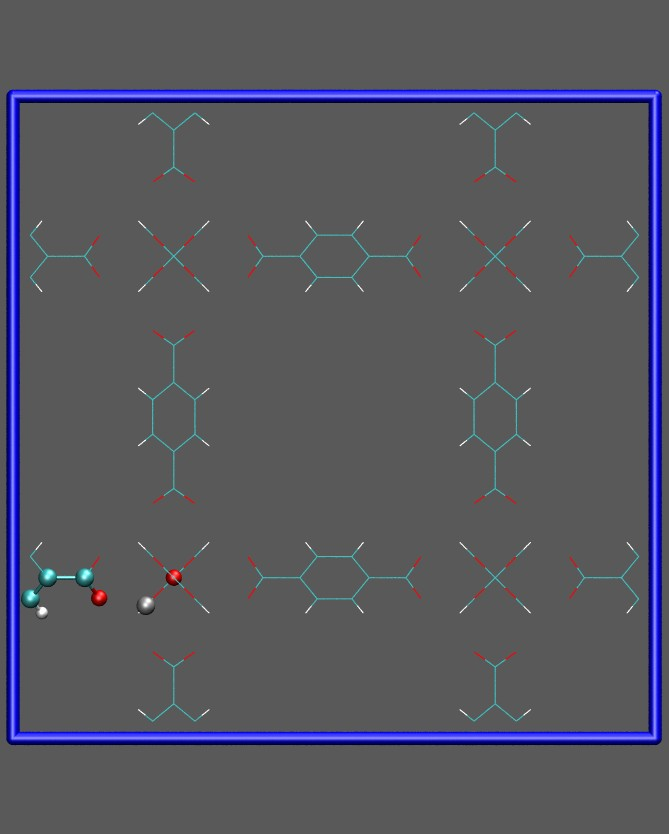
\includegraphics[width=7.5cm]{./InputFiles/IRMOF-1-asymmetric.jpg}}
   \subfloat[The full unit cell of IRMOF-1 has 424 atoms.]{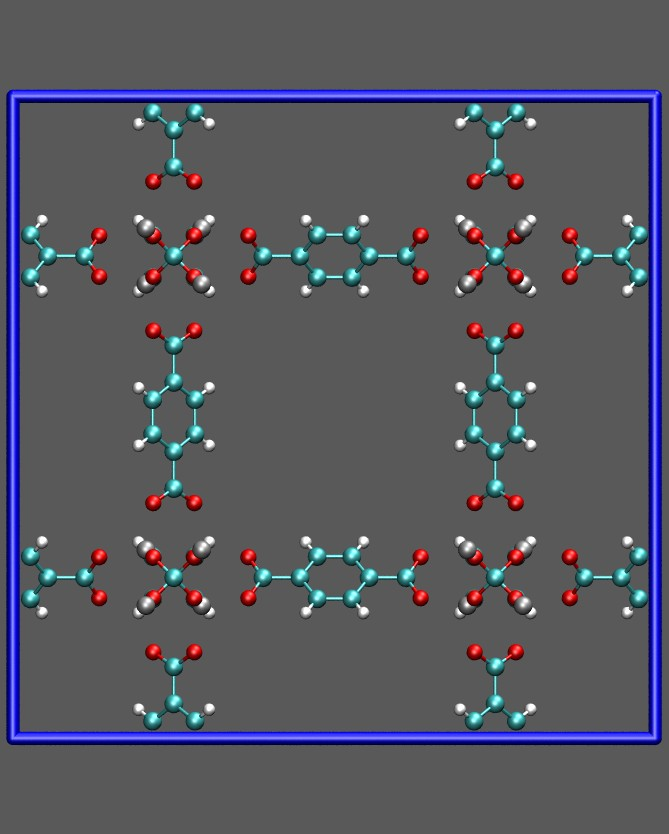
\includegraphics[width=7.5cm]{./InputFiles/IRMOF-1.jpg}}
  \caption{Asymmetric unit cells: the left figure shows the seven crystallographicly different atoms in the IRMOF-1 structure in
           ball-and-stick format. The `copies' (crystallographically identical atoms) are shown as lines. The right figure
           shows the full unit cell of IRMOF-1 in ball-and-stick.}
  \label{Fig: asymmetric}
\end{figure}

RASPA can then be run using:
\begin{verbatim}
    SimulationType       MonteCarlo
    NumberOfCycles       0
    InitializationCycles 0

    Forcefield           GenericMOFs

    Framework     0
    FrameworkName IRMOF-1
    UnitCells     1 1 1
\end{verbatim}
and in the directory \verb=`Movies/System_0/i'= several files appear: 
\begin{itemize}
\item{\verb=`Framework_0_initial_1_1_1.cif'=}\\
The framework in CIF-format at the start of the simulation.
\item{\verb=`Framework_0_initial_1_1_1_P1.cif'=}\\
The framework in CIF-format at the start of the simulation converted to P1 (no symmetry).
\item{\verb=`Framework_0_initial.pdb'=}\\
The framework in PDB-format at the start of the simulation converted to P1 (no symmetry).
\end{itemize}
The files named `final' are the structures at the end of the simulation. There are several programs that can read and view CIF-files:
e.g. Jmol (free), Mercury (free), Crystal Maker (commercial, free demo), Materials Studio (commercial), and Gaussview (commercial).
The PDB-files can be viewed in the freely available VMD-program.
\begin{center}
\shadowbox{
\begin{minipage}{\linewidth}
 Tip: always double check the \verb=`Framework_0_initial_1_1_1_P1.cif'=, if you see something strange then check 
  \verb=`_symmetry_space_group_name_Hall'= and the fractional positions.
\end{minipage}}
\end{center}


Space group 225 has 192 elements and the first 10 elements look like (see the file `src/spacegroup.c' for the complete set):
\begin{align*}
  x'&=x  \qquad &y'&=y   \qquad &z'&=z\\
  x'&=-x \qquad &y'&=-y  \qquad &z'&=z\\
  x'&=-x \qquad &y'&=y   \qquad &z'&=-z\\
  x'&=x  \qquad &y'&=-y  \qquad &z'&=-z\\
  x'&=z  \qquad &y'&=x   \qquad &z'&=y\\
  x'&=z  \qquad &y'&=-x  \qquad &z'&=-y\\
  x'&=-z \qquad &y'&=-x  \qquad &z'&=y\\
  x'&=-z \qquad &y'&=x   \qquad &z'&=-y\\
  x'&=y; \qquad &y'&=z   \qquad &z'&=x\\
  x'&=-y \qquad &y'&=z   \qquad &z'&=-x\\
  x'&=y  \qquad &y'&=-z  \qquad &z'&=-x\\
  \dots
\end{align*}
The procedure to generate a unit cell is to loop over the elements of the spacegroup and the atoms in the asymmetric unit cell, and to
apply simply all the rule. For each new $x',y',z'$ position a check is needed whether the same position has already been added
(doubles have to be removed). After this procedure the 7 positions have been expanded to 424 positions. The fractional positions
are transformed in the final step to Cartesian positions.



\subsection{Fractional occupancies in zeolites}

The procedure from asymmetric to full unit cell is rather simple when the fractional occupancies are unity. However, quite often there
is some disorder the type of atoms. For example, in zeolites like FAU the Si/Al ratio is specified, but it is unknown where the aluminum
actually is. Zeolite X is faujasite with a high amount of aluminum. The FAU structure with a Si/Al ratio of unity is given by
\begin{verbatim}
     data_NaX
     
     _audit_creation_method RASPA-1.0
     _audit_creation_date 2011-2-20
     _audit_author_name 'David Dubbeldam'
     
     _cell_length_a    25.099
     _cell_length_b    25.099
     _cell_length_c    25.099
     _cell_angle_alpha 90
     _cell_angle_beta  90
     _cell_angle_gamma 90
     _cell_volume      14273.9
     
     _symmetry_cell_setting          cubic
     _symmetry_space_group_name_Hall '-F 2uv 2vw 3'
     _symmetry_space_group_name_H-M  'F d -3'
     _symmetry_Int_Tables_number     203
     
     loop_
     _atom_site_label
     _atom_site_type_symbol
     _atom_site_fract_x
     _atom_site_fract_y
     _atom_site_fract_z
     Si1      Si4+  -0.05381   0.12565   0.03508
     Al1      Al3+  -0.05524   0.03639   0.12418
     O1       O2-   -0.1099    0.0003    0.1056 
     O2       O2-   -0.0011   -0.0028    0.1416 
     O3       O2-   -0.0346    0.0758    0.0711 
     O4       O2-   -0.0693    0.0726    0.18   
\end{verbatim}
Now the aluminum and silicon are alternating and L\"owestein rule is obeyed. For higher Si/Al ratios
the `Al' position is fractionally occupied and a certain percentage might actually be silicon. The
procedure here is to first generate the full unit cell of FAU with 96 aluminum (the maximum amount)
and judiciously replace aluminum by silicon in the full unit cell.

\begin{verbatim}
     SimulationType                MC
     NumberOfCycles                0
     NumberOfInitializationCycles  0
     PrintEvery                    10
     
     Forcefield                    Local
     
     Substitute 0 Al1 Si1
     Substitute 5 Al1 Si1
     Substitute 10 Al1 Si1
     Substitute 15 Al1 Si1
     Substitute 20 Al1 Si1
     RandomlySubstitute 75 Al1 Si1
     
     Framework 0
     FrameworkName NaX
     UnitCells 1 1 1
     ExternalTemperature 300.0
\end{verbatim}

It reads the CIF-file which is Nax with 96 aluminum. You can use two types of commands to replace an atom:
\begin{itemize}
\item{Substitute}\\
For example. \verb=Substitute 10 Al1 Si1= means replace the 10th \verb=Al1= by \verb=Si1=.
\item{RandomlySubstitute}\\
For example, \verb=RandomlySubstitute 75 Al1 Si1= means randomly substitute 75 \verb=Al1= by \verb=Si1=.
\end{itemize}

When you do them both, first the fixed rules are substituted and next the random ones with the `leftovers'.
The first one `Substitute' is useful to always have the same structure. You could make a random structure once, look in the output which Al was substituted and use the next time the `Substitute' command.
In this way, you always work with the spacegroup NaX structure (not in P1) which is afterwards change by specifying rules.

More problematic are when several atoms have fractional occupancies lower than unity. Consider IRMOF-8 shown in Fig. \ref{Fig: IRMOF-8}.
The linker molecules are disordered over two possible positions. One of these needs to be selected per linker. First the unit cell
is generated from the asymmetric unit cell and subsequently the unit cell needs to be edited. Program which can do just that are
Materials Studio, Gaussview, etc. After the cell has been created and edited, the file needs to be placed
in `structures/mofs/cif'. Structures with disorder needs to be created at unit cell level (P1).

Even more difficult is MOF-{\bf 1}. Here the cif-file also contains several possibilities, but is not a priori known which ones to choose, i.e.
what is the structure of the Dabco unit (1,4-diazabicyclo[2.2.2]octane) within the framework? One possibility is to choose a structure
and use a quantum code and minimize the periodic unit cell. The result is shown in Fig. \ref{Fig: cif vs dmol}.

Note that all these procedures are necessary, but it is still an open question, especially for MOFs, whether you can keep the framework rigid or not.
However, it is very hard to calibrate a flexible framework model and for this a substantial amount of reliable experimental data is required.

\subsection{Format of the framework atoms}

The atom-types in CIF-files are constructed from the name of the element and an identifier, e.g.\ \verb=`C10'= carbon type 10.
Usually these carbon atoms are different because they have either different charges or different Van der Waals parameters.

Sometimes a force field is defined to have interactions on an atom-type which depends on its neighbors. For example, the oxygen atom is different
whether it is connected to a silicon or to an aluminum atom. Therefore the atom are labelled using
\begin{verbatim}
ModifyFrameworkAtomConnectedTo O1 Oa1 Al1
ModifyFrameworkAtomConnectedTo O2 Oa2 Al1
ModifyFrameworkAtomConnectedTo O3 Oa3 Al1
ModifyFrameworkAtomConnectedTo O4 Oa4 Al1
\end{verbatim}
which modifies \verb=`O1'= to \verb=zOa1'= when connected to \verb=`Al1'=, etc.
In the CIF-file you can list the new framework atom with unknown position \verb=`?'=.
\begin{verbatim}
     loop_
     _atom_site_label
     _atom_site_type_symbol
     _atom_site_fract_x
     _atom_site_fract_y
     _atom_site_fract_z
     Si1      Si4+  -0.05381   0.12565   0.03508
     Al1      Al3+  -0.05524   0.03639   0.12418
     O1       O2-   -0.1099    0.0003    0.1056 
     O2       O2-   -0.0011   -0.0028    0.1416 
     O3       O2-   -0.0346    0.0758    0.0711 
     O4       O2-   -0.0693    0.0726    0.18   
     Oa1      O2-    ?         ?         ?      
     Oa2      O2-    ?         ?         ?      
     Oa3      O2-    ?         ?         ?      
     Oa4      O2-    ?         ?         ?      
\end{verbatim}
Alternatively, you can list the atom types \verb=`Oa1'=--\verb=`Oa4'= in your \verb=`pseudo_atoms.def'= file.

Other times a force field is defined as
\begin{verbatim}
     # rules to overwrite
     0
     # number of defined interactions
     4
     # type      type2       interaction
     O           O           lennard-jones     29.4338257        3.062219744
     O           Si          lennard-jones     49.05711264       3.483346249
     Si          Si          lennard-jones     81.76308187       3.962387454
     CH4_sp3     O           lennard-jones    115.00             3.47
     # mixing rules to overwrite
     0
\end{verbatim}
Here, we have that all oxygens in the framework are of the same type, and all silicon is of the same type.
In this case, we would like to map \verb=`O1'=, \verb=`O2'=, \verb=`O3'=, etc.\ to \verb=`O'=,
and \verb=`Si1'=, \verb=`Si2'=, etc.\ to \verb=`Si'=.
You can acgieve this using
\begin{verbatim}
     RemoveAtomNumberCodeFromLabel yes
\end{verbatim}

Suppose you want to use MFI with only \verb=`O'= and \verb=`Si'=. MFI is defined using 
\begin{verbatim}
     Si1      Si4+   0.42238   0.0565   -0.33598
     Si2      Si4+   0.30716   0.02772  -0.1893 
     \dots
     O1       O2-    0.3726    0.0534   -0.2442 
     O2       O2-    0.3084    0.0587   -0.0789 
     \dots
\end{verbatim}


The force field in \verb=`force_field.def'=
\begin{verbatim}
     # rules to overwrite
     0
     # number of defined interactions
     1
     # type      type2       interaction
     CH4_sp3     O           lennard-jones    115.00          3.47
     # mixing rules to overwrite
     0
\end{verbatim}
The \verb=`pseudo_atom.def'=
\begin{scriptsize}
\begin{verbatim}
     #number of pseudo atoms
     3
     #type      print   as  scatt mass       charge  polarization B-factor radii   connectivity  anisotropic anisotropic-type   tinker-type
     O          yes      O     O  15.9994   -1.025   0.0          1.0      0.5     2             0           absolute           0
     Si         yes     Si    Si  28.0855    2.05    0.0          1.0      1.18    4             0           absolute           0
     CH4_sp3    yes      C     C  16.04246   0.0     0.0          1.0      1.00    0             0           absolute           0
\end{verbatim}
\end{scriptsize}
and the output file will show:
\begin{scriptsize}
\begin{verbatim}
     Pseudo atoms: 2
     ===========================================================================
     Pseudo Atom[   0] Name Si       Oxydation:          Element: Si4+ pdb-name: Si   Scat. Types: 111  14 Mass=28.085498706 B-factor:0.000
                      Charge=2.050     Polarization=0.017    [A^3] (considered a charged atom and no polarization)  Interactions:  no
                      Anisotropic factor:    0.000 [-] (Absolute), Radius:    1.110 [A]
     Pseudo Atom[   1] Name O        Oxydation:          Element: O2-  pdb-name: O    Scat. Types: 105   8 Mass=15.999404927 B-factor:0.000
                      Charge=-1.025    Polarization=3.880    [A^3] (considered a charged atom and no polarization)  Interactions:  no
                      Anisotropic factor:    0.000 [-] (Absolute), Radius:    0.660 [A]
\end{verbatim}
\end{scriptsize}


\begin{figure}[p]
  \centering
   \subfloat[The IRMOF-8 structure as directly computed from the asymmetric positions and the space group.]{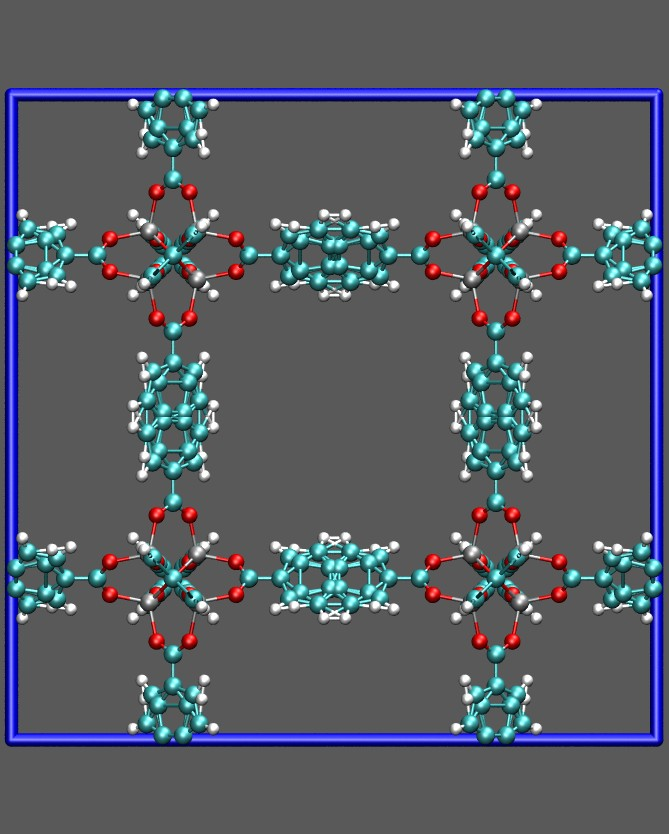
\includegraphics[width=6.0cm]{./InputFiles/IRMOF-8-full.jpg}}
   \hskip 1cm
   \subfloat[The IRMOF-8 after making a selection, shown is only one of the possibilities.]{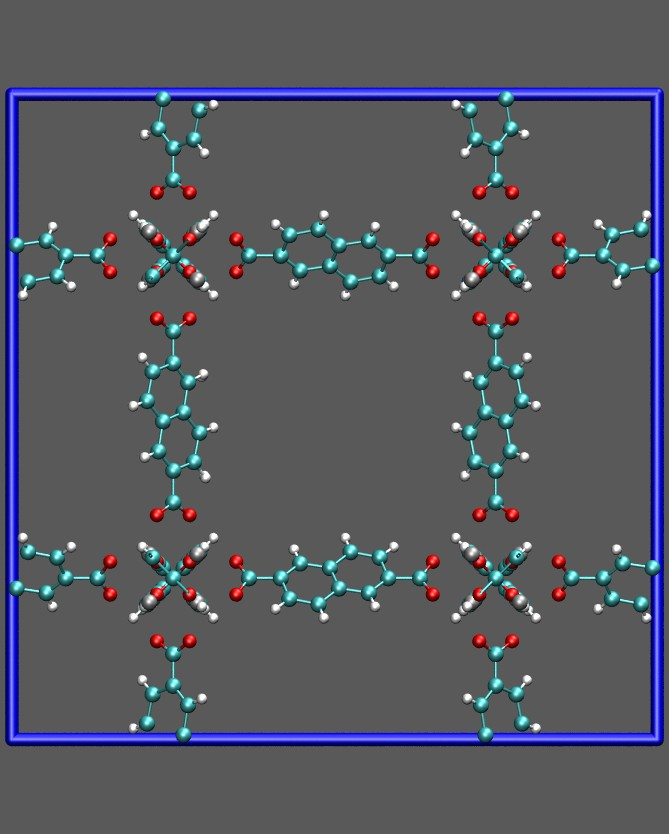
\includegraphics[width=6.0cm]{./InputFiles/IRMOF-8.jpg}}
  \caption{IRMOF-8 has linkers which are disordered, the linker atoms have a fractional occupancy of 0.5, The atoms however are not individually disorder and
           there are two disordered linker, one out of two possibilities needs to be selected per linker position.}
  \label{Fig: IRMOF-8}
  \centering
   \subfloat[The MOF-{\bf 1} structure from the cif-file.]{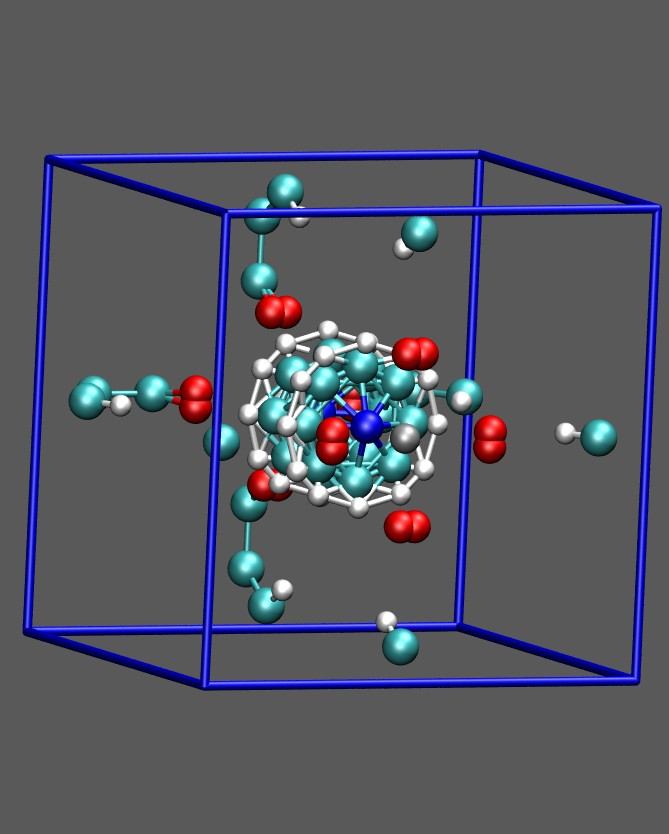
\includegraphics[width=6.0cm]{./InputFiles/MOF-1-cif.jpg}}
   \hskip 1cm
   \subfloat[The MOF-{\bf 1} structure edited and optimized with the quantum program dmol
                            (plane wave code).]{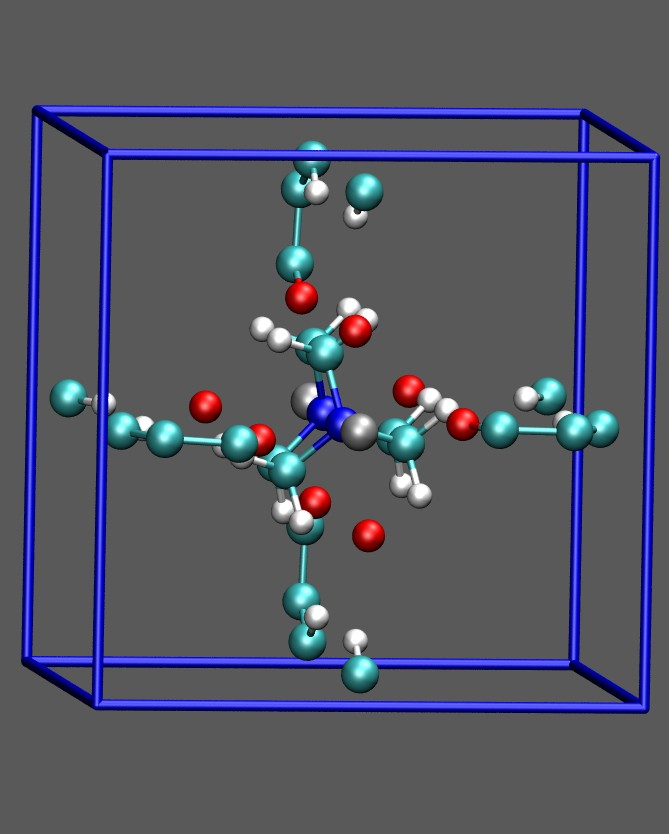
\includegraphics[width=6.0cm]{./InputFiles/MOF-1-dmol.jpg}}
  \caption{The MOF-1 structure is synthesized as [Zn$_2$(1,4-bdc)2(Dabco)]. The Dabco (1,4-diazabicyclo[2.2.2]octane) is very
          disordered with occupancies of 0.38 for the carbon and 0.5 for the hydrogen. The cif-file shown on the left shows all
          possibilities on top of each other. Here, just choosing one of the possibilities
          is difficult and it is not obvious which atoms to select. The brute force method is to select one possible choice and
          use a quantum plane wave for periodic structures and optimize the full unit cell. In this case it is feasible because
          of the low amount of atoms in the unit cell (only 54 atoms).}
  \label{Fig: cif vs dmol}
\end{figure}

\subsection{Typing the atoms of the framework}

Atoms from a pdb- or cif-file are usually labeled e.g. `C' for a carbon atom. In many force fields different carbon types have different charges.
It is necessary to `type' the structure and RASPA contains tools to do this. Let's assume the original structure always contains elements like `H', `C',
`N', `O', etc. and we want to type them `Mof\_Ha', `Mof\_Hb', etc. A force field type called `Typing' preexists. It only defines the `pseudo\_atoms.def' file:
\begin{small}
\begin{verbatim}
     #number of pseudo atoms
     43
     #type      print   as  scat     mass       charge    polarization B-factor radii  connectivity
     UNIT       no      H      H     1.0        1.0       0.0          1.0      1.0    0
     He         yes     He     He    4.002602   0.0       0.0          1.0      1.0    0
     Zn         yes     Zn1    Zn    65.37      0.0       0.0          1.0      1.448  0
     Zn1        yes     Zn1    Zn    65.37      0.0       0.0          1.0      1.448  0
     Cu         yes     Cu1    Cu    63.546     0.0       0.0          1.0      1.4    0
     Cu1        yes     Cu1    Cu    63.546     0.0       0.0          1.0      1.4    0
     O          yes     O      O     15.9994    0.0       0.0          1.0      0.68   2
     O1         yes     O1     O     15.9994    0.0       0.0          1.0      0.68   2
     O2         yes     O2     O     15.9994    0.0       0.0          1.0      0.68   2
     O3         yes     O3     O     15.9994    0.0       0.0          1.0      0.68   2
     O4         yes     O4     O     15.9994    0.0       0.0          1.0      0.68   2
     C          yes     C      C     12.0107    0.0       0.0          1.0      0.720  0
     C1         yes     C1     C     12.0107    0.0       0.0          1.0      0.720  0
     C2         yes     C2     C     12.0107    0.0       0.0          1.0      0.720  0
     C3         yes     C3     C     12.0107    0.0       0.0          1.0      0.720  0
     C4         yes     C4     C     12.0107    0.0       0.0          1.0      0.720  0
     C5         yes     C5     C     12.0107    0.0       0.0          1.0      0.720  0
     C6         yes     C6     C     12.0107    0.0       0.0          1.0      0.720  0
     C7         yes     C7     C     12.0107    0.0       0.0          1.0      0.720  0
     C8         yes     C8     C     12.0107    0.0       0.0          1.0      0.720  0
     C9         yes     C9     C     12.0107    0.0       0.0          1.0      0.720  0
     C10        yes     C10    C     12.0107    0.0       0.0          1.0      0.720  0
     C11        yes     C11    C     12.0107    0.0       0.0          1.0      0.720  0
     C12        yes     C12    C     12.0107    0.0       0.0          1.0      0.720  0
     C13        yes     C13    C     12.0107    0.0       0.0          1.0      0.720  0
     C14        yes     C14    C     12.0107    0.0       0.0          1.0      0.720  0
     C15        yes     C15    C     12.0107    0.0       0.0          1.0      0.720  0
     C16        yes     C16    C     12.0107    0.0       0.0          1.0      0.720  0
     N          yes     N      N     14.00674   0.0       0.0          1.0      0.68   0
     N1         yes     N1     N     14.00674   0.0       0.0          1.0      0.68   0
     N2         yes     N2     N     14.00674   0.0       0.0          1.0      0.68   0
     N3         yes     N3     N     14.00674   0.0       0.0          1.0      0.68   0
     N4         yes     N4     N     14.00674   0.0       0.0          1.0      0.68   0
     H          yes     H      H     1.00794    0.0       0.0          1.0      0.320  0
     H1         yes     H1     H     1.00794    0.0       0.0          1.0      0.320  0
     H2         yes     H2     H     1.00794    0.0       0.0          1.0      0.320  0
     H3         yes     H3     H     1.00794    0.0       0.0          1.0      0.320  0
     H4         yes     H4     H     1.00794    0.0       0.0          1.0      0.320  0
     H5         yes     H5     H     1.00794    0.0       0.0          1.0      0.320  0
     H6         yes     H6     H     1.00794    0.0       0.0          1.0      0.320  0
     H7         yes     H7     H     1.00794    0.0       0.0          1.0      0.320  0
     H8         yes     H8     H     1.00794    0.0       0.0          1.0      0.320  0
     H9         yes     H9     H     1.00794    0.0       0.0          1.0      0.320  0
\end{verbatim}
\end{small}

As an example, let's type the structure `NU-100' \cite{Farha2010}. Figure \ref{Fig: NU-100 cluster} shows the NU-100 cluster with linkers and
metal-corners. The pictures shows the different types of atoms and has been used to compute CHelpG charges.
In the RASPA input-file you can use the typing command:
\begin{verbatim}
ModifyFrameworkAtomConnectedTo C Mof_Ca O
\end{verbatim}
Look for a `C' atom, check if it is connect to an `O' atom and if so, type it `Mof\_Ca'.
It is also possible to define two neighbors:
\begin{verbatim}
ModifyFrameworkAtomConnectedTo C Mof_Cc Mof_Cb Mof_Cb
\end{verbatim}
Look for an `C' atom, if it is connect to a `Mof\_Cb' and to another `Mof\_Cb' atom, then type is `Mof\_Cc'.

\begin{figure}[t]
  \centering
   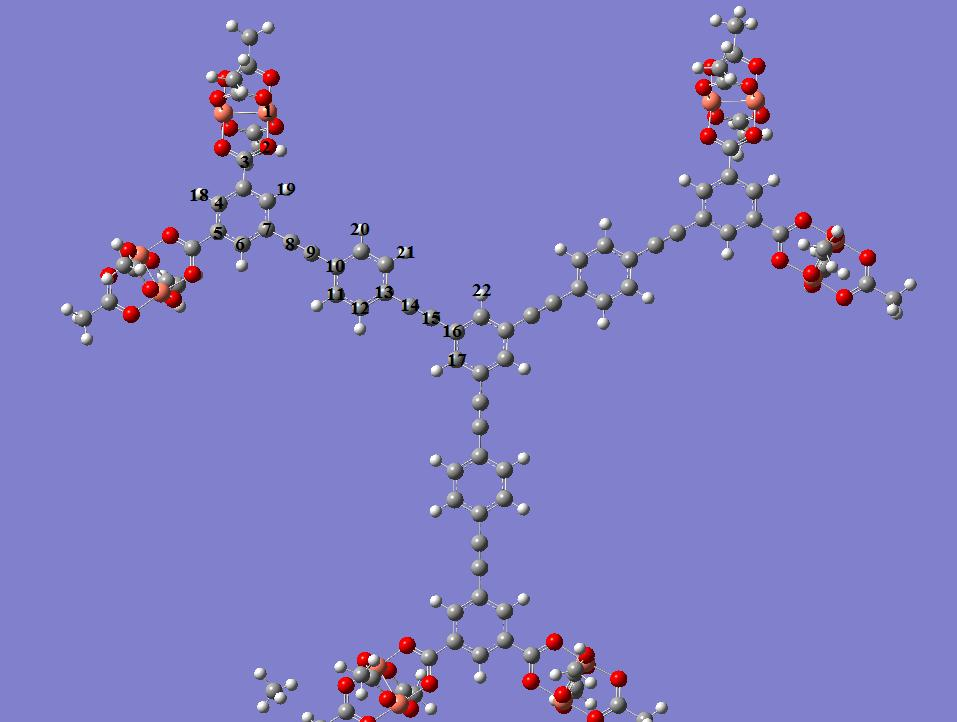
\includegraphics[width=15cm]{./InputFiles/NU-100.jpg}
  \caption{Cluster used for deriving partial charges on atoms in NU-100SP \cite{Farha2010}.}
  \label{Fig: NU-100 cluster}
\end{figure}


The input-file to type `NU-100' is
\begin{verbatim}
     SimulationType                   MC
     NumberOfCycles                   0
     
     Forcefield                       Local
     
     Framework 0
     FrameworkName NU-100SP
     UnitCells 1 1 1
     InputFileType cssr
     ExternalTemperature 298.0
     
     ModifyFrameworkAtomConnectedTo C C1 O
     ModifyFrameworkAtomConnectedTo C C2 C1
     ModifyFrameworkAtomConnectedTo C C3 C2 C2
     ModifyFrameworkAtomConnectedTo C C4 C2
     ModifyFrameworkAtomConnectedTo C C5 C4
     ModifyFrameworkAtomConnectedTo C C6 C5
     ModifyFrameworkAtomConnectedTo C C7 C6
     ModifyFrameworkAtomConnectedTo C C8 C7
     ModifyFrameworkAtomConnectedTo C C9 C8
     ModifyFrameworkAtomConnectedTo C C10 C9
     ModifyFrameworkAtomConnectedTo C C11 C10
     ModifyFrameworkAtomConnectedTo C C12 C11
     ModifyFrameworkAtomConnectedTo C C13 C12
     ModifyFrameworkAtomConnectedTo C C14 C13
     ModifyFrameworkAtomConnectedTo C C15 C14
     ModifyFrameworkAtomConnectedTo H H1 C3
     ModifyFrameworkAtomConnectedTo H H2 C4
     ModifyFrameworkAtomConnectedTo H H3 C9
     ModifyFrameworkAtomConnectedTo H H4 C10
     ModifyFrameworkAtomConnectedTo H H5 C15
     ModifyFrameworkAtomConnectedTo O O2 C1
     ModifyFrameworkAtomConnectedTo Cu Cu O2
\end{verbatim}

For MOFs, the easiest start-point to type is the carboxylate group. The carbon connected to the oxygen is typed `Mof\_Ca', the carbon
connected to `Mof\_Cb' is typed `Mof\_Cc'. The third line is important: the carbon should only be typed `Mof\_Cc' when it is connected
to an `Mof\_Cb' and another `Mof\_Cb'. This must be done like this, otherwise the atom which is above called `Mof\_Cd' would also
be wrongly labeled `Mof\_Cc'. After running RASPA, the `Movie'-directory contains the file `Framework\_intitial.cssr' which is the
cssr-file with complete typing. This file can be copied to `structures/mofs/cssr' and given an appropriate name.
Each pseudatom type can now be assigned a different charge in the `psuedo\_atoms.def' file of the 
`NU-100' forcefield.

Note that the lines containing the typing-rules  are performed top to bottom and in later rules one can use the new names of the previous rules.


\section{Using CIF-files}

\subsection{Definition of CIF-files}

CIF files present crystallographic data in an human readable free format. Let's look at an example:

\begin{footnotesize}
\begin{verbatim}
data_FAU_SI

_audit_creation_method RASPA-1.0
_audit_creation_date 2011-2-19
_audit_author_name 'David Dubbeldam'

_citation_author_name        'J.J. Hriljac, M.M. Eddy, A.K. Cheetham, J.A. Donohue,  and G.J. Ray'
_citation_title              'Powder Neutron Diffraction and Si-29 MAS NMR Studies of Siliceous Zeolite-Y'
_citation_journal_abbrev     'J. Solid State Chem.'
_citation_journal_volume     106
_citation_page_first         66
_citation_page_last          72
_citation_year               1993

_cell_length_a    24.2576
_cell_length_b    24.2576
_cell_length_c    24.2576
_cell_angle_alpha 90
_cell_angle_beta  90
_cell_angle_gamma 90
_cell_volume      14273.9

_symmetry_cell_setting          cubic
_symmetry_space_group_name_Hall '-F 4vw 2vw 3'
_symmetry_space_group_name_H-M  'F d -3 m'
_symmetry_Int_Tables_number     227

loop_
_symmetry_equiv_pos_as_xyz
 'x,y,z'
 '-x+3/4,-y+1/4,z+1/2'
  ................
  ................
  ................
 'z,-y+3/4,-x+3/4'
 'z+1/2,y+1/2,x'

loop_
_atom_site_label
_atom_site_type_symbol
_atom_site_fract_x
_atom_site_fract_y
_atom_site_fract_z
_atom_site_charge
_atom_site_polarization
Si1      Si4+  -0.05392   0.1253    0.03589   2.05    0
O1       O2-    0        -0.10623   0.10623  -1.025   0
O2       O2-   -0.00323  -0.00323   0.14066  -1.025   0
O3       O2-    0.0757    0.0757   -0.03577  -1.025   0
O4       O2-    0.07063   0.07063   0.32115  -1.025   0
\end{verbatim}
\end{footnotesize}

The `data\_' string signal the start of a data block. Each data block corresponds to a different structures, and typically only one structure is present (although it
possible to combine more than one structure in a single file).
The CIF instructions are divided into \emph{data name categories}, such as `\_atom\_site\_' to describe atomic site parameters, `\_cell\_'
to describe the cell parameters, `\_symmetry\_' to specify  space group symmetry, etc.
CIF data names begin with an underscore. For some data name the data can be provided using a list of data items. Such data items are preceded by a `loop\_' string.
The `\_atom\_site\_' section is typical example. The order of the data items correspond to the order in which the actual data is provided.

A nice feature of CIFs is that one can easily extend the syntax to include nom-standard data item. For example. in the `\_atom\_site\_' section,
the data items `\_atom\_site\_label', `\_atom\_site\_type\_symbol', `\_atom\_site\_fract\_x', `\_atom\_site\_fract\_y', `\_atom\_site\_charge' belong to the official CIF specification,
but `\_atom\_site\_charge', `\_atom\_site\_polarization', `\_atom\_site\_anisotropic\_displacement', `\_atom\_site\_anisotropic\_type',
and `\_atom\_site\_print\_to\_pdb' have been added in RASPA CIFs. Used in this fashion, they provide a replacement for the `pseudo\_atoms.def' file.
Note that if a `pseudo\_atoms.def' file is used, the value in that file will have preference over the CIF-file values (if they both define the same atom-type).

\subsection{What charge definition is used? `pseudo\_atom.def' or from the CIF-file?}

For adsorbates the charges are defined via the atom-type in the `pseudo\_atom.def' file.
For the framework, there are several scenarios:
\begin{itemize}
\item{define charges via the CIF-file}\\
If you want a possibly different charge for each atom, then use the option:
\begin{verbatim}
  UseChargesFromCIFFile yes
\end{verbatim}
and define the charge using the field `\_atom\_site\_charge' in the CIF-file.
Atom-types from the CIF-file that are not defined in the `pseudo\_atom.def' are automatically added, atoms that are already defined as a type in
the `pseudo\_atom.def' get the charge from the CIF-file. In the output-file in the list of pseudo-atoms you will see e.g.
\begin{verbatim}
  Charge=0.111115012    (av)
\end{verbatim}
which signals that for this atom-type the averages charge is listed (because each atom potentially can have a different value in this case).
This is a typical case for simulations based on CHelpG charges from quantum.
\item{define charges via the `pseudo\_atom.def' file}\\
If you want the same charge for all atoms of the atom-type, then you can list all of these in the `pseudo\_atom.def' file and use
\begin{verbatim}
  UseChargesFromCIFFile no
\end{verbatim}
which is the default. Any atoms with a type known in the CIF-file will get a charge given in the `pseudo\_atom.def' file; atoms of unknown type
will be added to the pseudo-atoms but with a charge of zero. The latter is probably not what you want, so make sure you have listed all atom type in `pseudo\_atom.def' file.
\item{Define charges using `Charge Equilibration'}\\
No matter what you define in the `pseudo\_atom.def' or CIF-file, the charges will be recompute using the charge-equilbration scheme of Wilmer and Snurr.
\end{itemize}

\begin{center}
\begin{shadedbox}
Tip: the charges that are actually used in the simulation are listed as the column `\_atom\_site\_charge'
in the file `Movies/System\_0/Framework\_0\_initial\_P1.cif'.
 Also, check the ouput-file for the net-charge of the framework, and the smallest and largest charge it found, e.g.\
           \begin{verbatim}
             Framework has net charge: 0.000000
             largest charge : 0.931455
             smallest charge: -0.626799
           \end{verbatim}
\end{shadedbox}
\end{center}

\subsection{How to choose atom-types?}

The FAU structure above was defined with atom types: `Si1', `O1', `O2', `O3', and `O4'. Using the option:
\begin{verbatim}
  RemoveAtomNumberCodeFromLabel yes
\end{verbatim}
these 5 types will be reduces to 2: `Si' and `O'. There are advantages and disadvantages to each of the options:
\begin{itemize}
\item{Specific types}\\
  Use if
  \begin{enumerate}
    \item{You want RDF between the adsorbate atoms and the specific framework atoms.}   
    \item{If you have different VDW parameters for each specific framework atom (so `O1', `O2', `O3', `O4' would have different VDW parameters).}
  \end{enumerate}
\item{Reduced types}\\
  Use if you are not interested in the difference between `O1', \dots, `O4', but only have a single VDW parameter set for that atom type `O'.
  Note: you can still list different charges for each of these atoms in the CIF-file.
  This options avoid excessive number of pseudo-atoms, which can clutter the output, and avoids having lots of different RDFs (and manually having to averages these afterwards).
\end{itemize}


\newpage
\clearpage
\subsection*{Appendix: space group information}

\begin{center}
\begin{small}
\begin{longtable}{|l|l|l|l|l|l|l|l|l|l|l|}
\hline
\multicolumn{10}{|>{\columncolor{orange-red}}c|}{triclinic}\\
\hline
\rowcolor{niceyellow}
id & Int. Nr. & long Hermann-    & Hall name & cell choice & centered &\# & Chiral & Centric & Enantio-\\
\rowcolor{niceyellow}
   &          & Mauguin name     &           &             &          &   &        &         & morphic\\
\hline
1 &1 &P 1 &P 1 &cell choice 1 &primitive &1 &yes &no &no \\ 
2 &2 &P -1 &-P 1 &cell choice 1 &primitive &2 &yes &no &no \\ 
\hline
\caption{Triclinic spacegroup information.}
\end{longtable}


\begin{longtable}{|l|l|l|l|l|l|l|l|l|l|l|}
\hline
\multicolumn{10}{|>{\columncolor{orange-red}}c|}{monoclinic}\\
\hline
\rowcolor{niceyellow}
id & Int. Nr. & long Hermann-    & Hall name & cell choice & centered &\# & Chiral & Centric & Enantio-\\
\rowcolor{niceyellow}
   &          & Mauguin name     &           &             &          &   &        &         & morphic\\
\hline
3 &3 &P 1 2 1 &P 2y &unique axis b &primitive &2 &no &yes &no \\ 
4 &3 &P 1 1 2 &P 2 &unique axis c &primitive &2 &no &yes &no \\ 
5 &3 &P 2 1 1 &P 2x &unique axis a &primitive &2 &no &yes &no \\ 
6 &4 &P 1 21 1 &P 2yb &unique axis b &primitive &2 &no &yes &no \\ 
7 &4 &P 1 1 21 &P 2c &unique axis c &primitive &2 &no &yes &no \\ 
8 &4 &P 21 1 1 &P 2xa &unique axis a &primitive &2 &no &yes &no \\ 
9 &5 &C 1 2 1 &C 2y &b, cell choice 1 &c &4 &no &yes &no \\ 
10 &5 &A 1 2 1 &A 2y &b, cell choice 2 &a &4 &no &yes &no \\ 
11 &5 &I 1 2 1 &I 2y &b, cell choice 3 &body &4 &no &yes &no \\ 
12 &5 &A 1 1 2 &A 2 &c, cell choice 1 &a &4 &no &yes &no \\ 
13 &5 &B 1 1 2 &B 2 &c, cell choice 2 &b &4 &no &yes &no \\ 
14 &5 &I 1 1 2 &I 2 &c, cell choice 3 &body &4 &no &yes &no \\ 
15 &5 &B 2 1 1 &B 2x &a, cell choice 1 &b &4 &no &yes &no \\ 
16 &5 &C 2 1 1 &C 2x &a, cell choice 2 &c &4 &no &yes &no \\ 
17 &5 &I 2 1 1 &I 2x &a, cell choice 3 &body &4 &no &yes &no \\ 
18 &6 &P 1 m 1 &P -2y &unique axis b &primitive &2 &no &no &no \\ 
19 &6 &P 1 1 m &P -2 &unique axis c &primitive &2 &no &no &no \\ 
20 &6 &P m 1 1 &P -2x &unique axis a &primitive &2 &no &no &no \\ 
21 &7 &P 1 c 1 &P -2yc &b, cell choice 1 &primitive &2 &no &no &no \\ 
22 &7 &P 1 n 1 &P -2yac &b, cell choice 2 &primitive &2 &no &no &no \\ 
23 &7 &P 1 a 1 &P -2ya &b, cell choice 3 &primitive &2 &no &no &no \\ 
24 &7 &P 1 1 a &P -2a &c, cell choice 1 &primitive &2 &no &no &no \\ 
25 &7 &P 1 1 n &P -2ab &c, cell choice 2 &primitive &2 &no &no &no \\ 
26 &7 &P 1 1 b &P -2b &c, cell choice 3 &primitive &2 &no &no &no \\ 
27 &7 &P b 1 1 &P -2xb &a, cell choice 1 &primitive &2 &no &no &no \\ 
28 &7 &P n 1 1 &P -2xbc &a, cell choice 2 &primitive &2 &no &no &no \\ 
29 &7 &P c 1 1 &P -2xc &a, cell choice 3 &primitive &2 &no &no &no \\ 
30 &8 &C 1 m 1 &C -2y &b, cell choice 1 &c &4 &no &no &no \\ 
31 &8 &A 1 m 1 &A -2y &b, cell choice 2 &a &4 &no &no &no \\ 
32 &8 &I 1 m 1 &I -2y &b, cell choice 3 &body &4 &no &no &no \\ 
33 &8 &A 1 1 m &A -2 &c, cell choice 1 &a &4 &no &no &no \\ 
34 &8 &B 1 1 m &B -2 &c, cell choice 2 &b &4 &no &no &no \\ 
35 &8 &I 1 1 m &I -2 &c, cell choice 3 &body &4 &no &no &no \\ 
36 &8 &B m 1 1 &B -2x &a, cell choice 1 &b &4 &no &no &no \\ 
37 &8 &B m 1 1 &C -2x &a, cell choice 2 &c &4 &no &no &no \\ 
38 &8 &I m 1 1 &I -2x &a, cell choice 3 &body &4 &no &no &no \\ 
39 &9 &C 1 c 1 &C -2yc &b, cell choice 1 &c &4 &no &no &no \\ 
40 &9 &A 1 n 1 &A -2yab &b, cell choice 2 &a &4 &no &no &no \\ 
41 &9 &I 1 a 1 &I -2ya &b, cell choice 3 &body &4 &no &no &no \\ 
42 &9 &A 1 a 1 &A -2ya &-b, cell choice 1 &a &4 &no &no &no \\ 
43 &9 &C 1 n 1 &C -2yac &-b, cell choice 2 &c &4 &no &no &no \\ 
44 &9 &I 1 c 1 &I -2yc &-b, cell choice 3 &body &4 &no &no &no \\ 
45 &9 &A 1 1 a &A -2a &c, cell choice 1 &a &4 &no &no &no \\ 
46 &9 &B 1 1 n &B -2ab &c, cell choice 2 &b &4 &no &no &no \\ 
47 &9 &I 1 1 b &I -2b &c, cell choice 3 &body &4 &no &no &no \\ 
48 &9 &B 1 1 b &B -2b &-c, cell choice 1 &b &4 &no &no &no \\ 
49 &9 &A 1 1 n &A -2ab &-c, cell choice 2 &a &4 &no &no &no \\ 
50 &9 &I 1 1 a &I -2a &-c, cell choice 3 &body &4 &no &no &no \\ 
51 &9 &B b 1 1 &B -2xb &a, cell choice 1 &b &4 &no &no &no \\ 
52 &9 &C n 1 1 &C -2xac &a, cell choice 2 &c &4 &no &no &no \\ 
53 &9 &I c 1 1 &I -2xc &a, cell choice 3 &body &4 &no &no &no \\ 
54 &9 &C c 1 1 &C -2xc &-a, cell choice 1 &c &4 &no &no &no \\ 
55 &9 &B n 1 1 &B -2xab &-a, cell choice 2 &b &4 &no &no &no \\ 
56 &9 &I b 1 1 &I -2xb &-a, cell choice 3 &body &4 &no &no &no \\ 
57 &10 &P 1 2/m 1 &-P 2y &unique axis b &primitive &4 &yes &no &no \\ 
58 &10 &P 1 1 2/m &-P 2 &unique axis c &primitive &4 &yes &no &no \\ 
59 &10 &P 2/m 1 1 &-P 2x &unique axis a &primitive &4 &yes &no &no \\ 
60 &11 &P 1 21/m 1 &-P 2yb &unique axis b &primitive &4 &yes &no &no \\ 
61 &11 &P 1 1 21/m &-P 2c &unique axis c &primitive &4 &yes &no &no \\ 
62 &11 &P 21/m 1 1 &-P 2xa &unique axis a &primitive &4 &yes &no &no \\ 
63 &12 &C 1 2/m 1 &-C 2y &b, cell choice 1 &c &8 &yes &no &no \\ 
64 &12 &A 1 2/m 1 &-A 2y &b, cell choice 2 &a &8 &yes &no &no \\ 
65 &12 &I 1 2/m 1 &-I 2y &b, cell choice 3 &body &8 &yes &no &no \\ 
66 &12 &A 1 1 2/m &-A 2 &c, cell choice 1 &a &8 &yes &no &no \\ 
67 &12 &B 1 1 2/m &-B 2 &c, cell choice 2 &b &8 &yes &no &no \\ 
68 &12 &I 1 1 2/m &-I 2 &c, cell choice 3 &body &8 &yes &no &no \\ 
69 &12 &B 2/m 1 1 &-B 2x &a, cell choice 1 &b &8 &yes &no &no \\ 
70 &12 &C 2/m 1 1 &-C 2x &a, cell choice 2 &c &8 &yes &no &no \\ 
71 &12 &I 2/m 1 1 &-I 2x &a, cell choice 3 &body &8 &yes &no &no \\ 
72 &13 &P 1 2/c 1 &-P 2yc &b, cell choice 1 &primitive &4 &yes &no &no \\ 
73 &13 &P 1 2/n 1 &-P 2yac &b, cell choice 2 &primitive &4 &yes &no &no \\ 
74 &13 &P 1 2/a 1 &-P 2ya &b, cell choice 3 &primitive &4 &yes &no &no \\ 
75 &13 &P 1 1 2/a &-P 2a &c, cell choice 1 &primitive &4 &yes &no &no \\ 
76 &13 &P 1 1 2/n &-P 2ab &c, cell choice 2 &primitive &4 &yes &no &no \\ 
77 &13 &P 1 1 2/b &-P 2b &c, cell choice 3 &primitive &4 &yes &no &no \\ 
78 &13 &P 2/b 1 1 &-P 2xb &a, cell choice 1 &primitive &4 &yes &no &no \\ 
79 &13 &P 2/n 1 1 &-P 2xbc &a, cell choice 2 &primitive &4 &yes &no &no \\ 
80 &13 &P 2/c 1 1 &-P 2xc &a, cell choice 3 &primitive &4 &yes &no &no \\ 
81 &14 &P 1 21/c 1 &-P 2ybc &b, cell choice 1 &primitive &4 &yes &no &no \\ 
82 &14 &P 1 21/n 1 &-P 2yn &b, cell choice 2 &primitive &4 &yes &no &no \\ 
83 &14 &P 1 21/a 1 &-P 2yab &b, cell choice 3 &primitive &4 &yes &no &no \\ 
84 &14 &P 1 1 21/a &-P 2ac &c, cell choice 1 &primitive &4 &yes &no &no \\ 
85 &14 &P 1 1 21/n &-P 2n &c, cell choice 2 &primitive &4 &yes &no &no \\ 
86 &14 &P 1 1 21/b &-P 2bc &c, cell choice 3 &primitive &4 &yes &no &no \\ 
87 &14 &P 21/b 1 1 &-P 2xab &a, cell choice 1 &primitive &4 &yes &no &no \\ 
88 &14 &P 21/n 1 1 &-P 2xn &a, cell choice 2 &primitive &4 &yes &no &no \\ 
89 &14 &P 21/c 1 1 &-P 2xac &a, cell choice 3 &primitive &4 &yes &no &no \\ 
90 &15 &C 1 2/c 1 &-C 2yc &b, cell choice 1 &c &8 &yes &no &no \\ 
91 &15 &A 1 2/n 1 &-A 2yab &b, cell choice 2 &a &8 &yes &no &no \\ 
92 &15 &I 1 2/a 1 &-I 2ya &b, cell choice 3 &body &8 &yes &no &no \\ 
93 &15 &A 1 2/a 1 &-A 2ya &-b, cell choice 1 &a &8 &yes &no &no \\ 
94 &15 &C 1 2/n 1 &-C 2yac &-b, cell choice 2 &c &8 &yes &no &no \\ 
95 &15 &I 1 2/c 1 &-I 2yc &-b, cell choice 3 &body &8 &yes &no &no \\ 
96 &15 &A 1 1 2/a &-A 2a &c, cell choice 1 &a &8 &yes &no &no \\ 
97 &15 &B 1 1 2/n &-B 2ab &c, cell choice 2 &b &8 &yes &no &no \\ 
98 &15 &I 1 1 2/b &-I 2b &c, cell choice 3 &body &8 &yes &no &no \\ 
99 &15 &B 1 1 2/b &-B 2b &-c, cell choice 1 &b &8 &yes &no &no \\ 
100 &15 &A 1 1 2/n &-A 2ab &-c, cell choice 2 &a &8 &yes &no &no \\ 
101 &15 &I 1 1 2/a &-I 2a &-c, cell choice 3 &body &8 &yes &no &no \\ 
102 &15 &B 2/b 1 1 &-B 2xb &a, cell choice 1 &b &8 &yes &no &no \\ 
103 &15 &C 2/n 1 1 &-C 2xac &a, cell choice 2 &c &8 &yes &no &no \\ 
104 &15 &I 2/c 1 1 &-I 2xc &a, cell choice 3 &body &8 &yes &no &no \\ 
105 &15 &C 2/c 1 1 &-C 2xc &-a, cell choice 1 &c &8 &yes &no &no \\ 
106 &15 &B 2/n 1 1 &-B 2xab &-a, cell choice 2 &b &8 &yes &no &no \\ 
107 &15 &I 2/b 1 1 &-I 2xb &-a, cell choice 3 &body &8 &yes &no &no \\ 
\hline
\caption{Monoclinic spacegroup information.}
\end{longtable}

\begin{longtable}{|l|l|l|l|l|l|l|l|l|l|l|}
\hline
\multicolumn{10}{|>{\columncolor{orange-red}}c|}{orthorhombic}\\
\hline
\rowcolor{niceyellow}
id & Int. Nr. & long Hermann-    & Hall name & cell choice & centered &\# & Chiral & Centric & Enantio-\\
\rowcolor{niceyellow}
   &          & Mauguin name     &           &             &          &   &        &         & morphic\\
\hline
108 &16 &P 2 2 2 &P 2 2 &cell choice 1 &primitive &4 &yes &yes &no \\ 
109 &17 &P 2 2 21 &P 2c 2 &abc &primitive &4 &yes &yes &no \\ 
110 &17 &P 21 2 2 &P 2a 2a &cab &primitive &4 &yes &yes &no \\ 
111 &17 &P 2 21 2 &P 2 2b &bca &primitive &4 &yes &yes &no \\ 
112 &18 &P 21 21 2 &P 2 2ab &abc &primitive &4 &yes &yes &no \\ 
113 &18 &P 2 21 21 &P 2bc 2 &cab &primitive &4 &yes &yes &no \\ 
114 &18 &P 21 2 21 &P 2ac 2ac &bca &primitive &4 &yes &yes &no \\ 
115 &19 &P 21 21 21 &P 2ac 2ab &cell choice 1 &primitive &4 &yes &yes &no \\ 
116 &20 &C 2 2 21 &C 2c 2 &abc &c &8 &yes &yes &no \\ 
117 &20 &A 21 2 2 &A 2a 2a &cab &a &8 &yes &yes &no \\ 
118 &20 &B 2 21 2 &B 2 2b &bca &b &8 &yes &yes &no \\ 
119 &21 &C 2 2 2 &C 2 2 &abc &c &8 &no &yes &no \\ 
120 &21 &A 2 2 2 &A 2 2 &cab &a &8 &no &yes &no \\ 
121 &21 &B 2 2 2 &B 2 2 &bca &b &8 &no &yes &no \\ 
122 &22 &F 2 2 2 &F 2 2 &cell choice 1 &face &16 &no &yes &no \\ 
123 &23 &I 2 2 2 &I 2 2 &cell choice 1 &body &8 &no &yes &no \\ 
124 &24 &I 21 21 21 &I 2b 2c &cell choice 1 &body &8 &no &yes &no \\ 
125 &25 &P m m 2 &P 2 -2 &abc &primitive &4 &no &no &no \\ 
126 &25 &P 2 m m &P -2 2 &cab &primitive &4 &no &no &no \\ 
127 &25 &P m 2 m &P -2 -2 &bca &primitive &4 &no &no &no \\ 
128 &26 &P m c 21 &P 2c -2 &abc &primitive &4 &no &no &no \\ 
129 &26 &P c m 21 &P 2c -2c &ba-c &primitive &4 &no &no &no \\ 
130 &26 &P 21 m a &P -2a 2a &cab &primitive &4 &no &no &no \\ 
131 &26 &P 21 a m &P -2 2a &-cba &primitive &4 &no &no &no \\ 
132 &26 &P b 21 m &P -2 -2b &bca &primitive &4 &no &no &no \\ 
133 &26 &P m 21 b &P -2b -2 &a-cb &primitive &4 &no &no &no \\ 
134 &27 &P c c 2 &P 2 -2c &abc &primitive &4 &no &no &no \\ 
135 &27 &P 2 a a &P -2a 2 &cab &primitive &4 &no &no &no \\ 
136 &27 &P b 2 b &P -2b -2b &bca &primitive &4 &no &no &no \\ 
137 &28 &P m a 2 &P 2 -2a &abc &primitive &4 &no &no &no \\ 
138 &28 &P b m 2 &P 2 -2b &ba-c &primitive &4 &no &no &no \\ 
139 &28 &P 2 m b &P -2b 2 &cab &primitive &4 &no &no &no \\ 
140 &28 &P 2 c m &P -2c 2 &-cba &primitive &4 &no &no &no \\ 
141 &28 &P c 2 m &P -2c -2c &bca &primitive &4 &no &no &no \\ 
142 &28 &P m 2 a &P -2a -2a &a-cb &primitive &4 &no &no &no \\ 
143 &29 &P c a 21 &P 2c -2ac &abc &primitive &4 &no &no &no \\ 
144 &29 &P b c 21 &P 2c -2b &ba-c &primitive &4 &no &no &no \\ 
145 &29 &P 21 a b &P -2b 2a &cab &primitive &4 &no &no &no \\ 
146 &29 &P 21 c a &P -2ac 2a &-cba &primitive &4 &no &no &no \\ 
147 &29 &P c 21 b &P -2bc -2c &bca &primitive &4 &no &no &no \\ 
148 &29 &P b 21 a &P -2a -2ab &a-cb &primitive &4 &no &no &no \\ 
149 &30 &P n c 2 &P 2 -2bc &abc &primitive &4 &no &no &no \\ 
150 &30 &P c n 2 &P 2 -2ac &ba-c &primitive &4 &no &no &no \\ 
151 &30 &P 2 n a &P -2ac 2 &cab &primitive &4 &no &no &no \\ 
152 &30 &P 2 a n &P -2ab 2 &-cba &primitive &4 &no &no &no \\ 
153 &30 &P b 2 n &P -2ab -2ab &bca &primitive &4 &no &no &no \\ 
154 &30 &P n 2 b &P -2bc -2bc &a-cb &primitive &4 &no &no &no \\ 
155 &31 &P m n 21 &P 2ac -2 &abc &primitive &4 &no &no &no \\ 
156 &31 &P n m 21 &P 2bc -2bc &ba-c &primitive &4 &no &no &no \\ 
157 &31 &P 21 m n &P -2ab 2ab &cab &primitive &4 &no &no &no \\ 
158 &31 &P 21 n m &P -2 2ac &-cba &primitive &4 &no &no &no \\ 
159 &31 &P n 21 m &P -2 -2bc &bca &primitive &4 &no &no &no \\ 
160 &31 &P m 21 n &P -2ab -2 &a-cb &primitive &4 &no &no &no \\ 
161 &32 &P b a 2 &P 2 -2ab &abc &primitive &4 &no &no &no \\ 
162 &32 &P 2 c b &P -2bc 2 &cab &primitive &4 &no &no &no \\ 
163 &32 &P c 2 a &P -2ac -2ac &bca &primitive &4 &no &no &no \\ 
164 &33 &P n a 21 &P 2c -2n &abc &primitive &4 &no &no &no \\ 
165 &33 &P b n 21 &P 2c -2ab &ba-c &primitive &4 &no &no &no \\ 
166 &33 &P 21 n b &P -2bc 2a &cab &primitive &4 &no &no &no \\ 
167 &33 &P 21 c n &P -2n 2a &-cba &primitive &4 &no &no &no \\ 
168 &33 &P c 21 n &P -2n -2ac &bca &primitive &4 &no &no &no \\ 
169 &33 &P n 21 a &P -2ac -2n &a-cb &primitive &4 &no &no &no \\ 
170 &34 &P n n 2 &P 2 -2n &abc &primitive &4 &no &no &no \\ 
171 &34 &P 2 n n &P -2n 2 &cab &primitive &4 &no &no &no \\ 
172 &34 &P n 2 n &P -2n -2n &bca &primitive &4 &no &no &no \\ 
173 &35 &C m m 2 &C 2 -2 &abc &c &8 &no &no &no \\ 
174 &35 &A 2 m m &A -2 2 &cab &a &8 &no &no &no \\ 
175 &35 &B m 2 m &B -2 -2 &bca &b &8 &no &no &no \\ 
176 &36 &C m c 21 &C 2c -2 &abc &c &8 &no &no &no \\ 
177 &36 &C c m 21 &C 2c -2c &ba-c &c &8 &no &no &no \\ 
178 &36 &A 21 m a &A -2a 2a &cab &a &8 &no &no &no \\ 
179 &36 &A 21 a m &A -2 2a &-cba &a &8 &no &no &no \\ 
180 &36 &B b 21 m &B -2 -2b &bca &b &8 &no &no &no \\ 
181 &36 &B m 21 b &B -2b -2 &a-cb &b &8 &no &no &no \\ 
182 &37 &C c c 2 &C 2 -2c &abc &c &8 &no &no &no \\ 
183 &37 &A 2 a a &A -2a 2 &cab &a &8 &no &no &no \\ 
184 &37 &B b 2 b &B -2b -2b &bca &b &8 &no &no &no \\ 
185 &38 &A m m 2 &A 2 -2 &abc &a &8 &no &no &no \\ 
186 &38 &B m m 2 &B 2 -2 &ba-c &b &8 &no &no &no \\ 
187 &38 &B 2 m m &B -2 2 &cab &b &8 &no &no &no \\ 
188 &38 &C 2 m m &C -2 2 &-cba &c &8 &no &no &no \\ 
189 &38 &C m 2 m &C -2 -2 &bca &c &8 &no &no &no \\ 
190 &38 &A m 2 m &A -2 -2 &a-cb &a &8 &no &no &no \\ 
191 &39 &A b m 2 &A 2 -2b &abc &a &8 &no &no &no \\ 
192 &39 &B m a 2 &B 2 -2a &ba-c &b &8 &no &no &no \\ 
193 &39 &B 2 c m &B -2a 2 &cab &b &8 &no &no &no \\ 
194 &39 &C 2 m b &C -2a 2 &-cba &c &8 &no &no &no \\ 
195 &39 &C m 2 a &C -2a -2a &bca &c &8 &no &no &no \\ 
196 &39 &A c 2 m &A -2b -2b &a-cb &a &8 &no &no &no \\ 
197 &40 &A m a 2 &A 2 -2a &abc &a &8 &no &no &no \\ 
198 &40 &B b m 2 &B 2 -2b &ba-c &b &8 &no &no &no \\ 
199 &40 &B 2 m b &B -2b 2 &cab &b &8 &no &no &no \\ 
200 &40 &C 2 c m &C -2c 2 &-cba &c &8 &no &no &no \\ 
201 &40 &C c 2 m &C -2c -2c &bca &c &8 &no &no &no \\ 
202 &40 &A m 2 a &A -2a -2a &a-cb &a &8 &no &no &no \\ 
203 &41 &A b a 2 &A 2 -2ab &abc &a &8 &no &no &no \\ 
204 &41 &B b a 2 &B 2 -2ab &ba-c &b &8 &no &no &no \\ 
205 &41 &B 2 c b &B -2ab 2 &cab &b &8 &no &no &no \\ 
206 &41 &C 2 c b &C -2ac 2 &-cba &c &8 &no &no &no \\ 
207 &41 &C c 2 a &C -2ac -2ac &bca &c &8 &no &no &no \\ 
208 &41 &A c 2 a &A -2ab -2ab &a-cb &a &8 &no &no &no \\ 
209 &42 &F m m 2 &F 2 -2 &abc &face &16 &no &no &no \\ 
210 &42 &F 2 m m &F -2 2 &cab &face &16 &no &no &no \\ 
211 &42 &F m 2 m &F -2 -2 &bca &face &16 &no &no &no \\ 
212 &43 &F d d 2 &F 2 -2d &abc &face &16 &no &no &no \\ 
213 &43 &F 2 d d &F -2d 2 &cab &face &16 &no &no &no \\ 
214 &43 &F d 2 d &F -2d -2d &bca &face &16 &no &no &no \\ 
215 &44 &I m m 2 &I 2 -2 &abc &body &8 &no &no &no \\ 
216 &44 &I 2 m m &I -2 2 &cab &body &8 &no &no &no \\ 
217 &44 &I m 2 m &I -2 -2 &bca &body &8 &no &no &no \\ 
218 &45 &I b a 2 &I 2 -2c &abc &body &8 &no &no &no \\ 
219 &45 &I 2 c b &I -2a 2 &cab &body &8 &no &no &no \\ 
220 &45 &I c 2 a &I -2b -2b &bca &body &8 &no &no &no \\ 
221 &46 &I m a 2 &I 2 -2a &abc &body &8 &no &no &no \\ 
222 &46 &I b m 2 &I 2 -2b &ba-c &body &8 &no &no &no \\ 
223 &46 &I 2 m b &I -2b 2 &cab &body &8 &no &no &no \\ 
224 &46 &I 2 c m &I -2c 2 &-cba &body &8 &no &no &no \\ 
225 &46 &I c 2 m &I -2c -2c &bca &body &8 &no &no &no \\ 
226 &46 &I m 2 a &I -2a -2a &a-cb &body &8 &no &no &no \\ 
227 &47 &P 2/m 2/m 2/m &-P 2 2 &cell choice 1 &primitive &8 &yes &no &no \\ 
228 &48 &P 2/n 2/n 2/n:1 &P 2 2 -1n &cell choice 1 &primitive &8 &yes &no &no \\ 
229 &48 &P 2/n 2/n 2/n:2 &-P 2ab 2bc &cell choice 2 &primitive &8 &yes &no &no \\ 
230 &49 &P 2/c 2/c 2/m &-P 2 2c &abc &primitive &8 &yes &no &no \\ 
231 &49 &P 2/m 2/a 2/a &-P 2a 2 &cab &primitive &8 &yes &no &no \\ 
232 &49 &P 2/b 2/m 2/b &-P 2b 2b &bca &primitive &8 &yes &no &no \\ 
233 &50 &P 2/b 2/a 2/n:1 &P 2 2 -1ab &cell choice 1 &primitive &8 &yes &no &no \\ 
234 &50 &P 2/b 2/a 2/n:2 &-P 2ab 2b &cell choice 2 &primitive &8 &yes &no &no \\ 
235 &50 &P 2/n 2/c 2/b:1 &P 2 2 -1bc &cab &primitive &8 &yes &no &no \\ 
236 &50 &P 2/n 2/c 2/b:2 &-P 2b 2bc &cab, cell choice 2 &primitive &8 &yes &no &no \\ 
237 &50 &P 2/c 2/n 2/a:1 &P 2 2 -1ac &bca &primitive &8 &yes &no &no \\ 
238 &50 &P 2/c 2/n 2/a:2 &-P 2a 2c &bca, cell choice 2 &primitive &8 &yes &no &no \\ 
239 &51 &P 21/m 2/m 2/a &-P 2a 2a &abc &primitive &8 &yes &no &no \\ 
240 &51 &P 2/m 21/m 2/b &-P 2b 2 &ba-c &primitive &8 &yes &no &no \\ 
241 &51 &P 2/b 21/m 2/m &-P 2 2b &cab &primitive &8 &yes &no &no \\ 
242 &51 &P 2/c 2/m 21/m &-P 2c 2c &-cba &primitive &8 &yes &no &no \\ 
243 &51 &P 2/m 2/c 21/m &-P 2c 2 &bca &primitive &8 &yes &no &no \\ 
244 &51 &P 21/m 2/a 2/m &-P 2 2a &a-cb &primitive &8 &yes &no &no \\ 
245 &52 &P 2/n 21/n 2/a &-P 2a 2bc &abc &primitive &8 &yes &no &no \\ 
246 &52 &P 21/n 2/n 2/b &-P 2b 2n &ba-c &primitive &8 &yes &no &no \\ 
247 &52 &P 2/b 2/n 21/n &-P 2n 2b &cab &primitive &8 &yes &no &no \\ 
248 &52 &P 2/c 21/n 2/n &-P 2ab 2c &-cba &primitive &8 &yes &no &no \\ 
249 &52 &P 21/n 2/c 2/n &-P 2ab 2n &bca &primitive &8 &yes &no &no \\ 
250 &52 &P 2/n 2/a 21/n &-P 2n 2bc &a-cb &primitive &8 &yes &no &no \\ 
251 &53 &P 2/m 2/n 21/a &-P 2ac 2 &abc &primitive &8 &yes &no &no \\ 
252 &53 &P 2/n 2/m 21/b &-P 2bc 2bc &ba-c &primitive &8 &yes &no &no \\ 
253 &53 &P 21/b 2/m 2/n &-P 2ab 2ab &cab &primitive &8 &yes &no &no \\ 
254 &53 &P 21/c 2/n 2/m &-P 2 2ac &-cba &primitive &8 &yes &no &no \\ 
255 &53 &P 2/n 21/c 2/m &-P 2 2bc &bca &primitive &8 &yes &no &no \\ 
256 &53 &P 2/m 21/a 2/n &-P 2ab 2 &a-cb &primitive &8 &yes &no &no \\ 
257 &54 &P 21/c 2/c 2/a &-P 2a 2ac &abc &primitive &8 &yes &no &no \\ 
258 &54 &P 2/c 21/c 2/b &-P 2b 2c &ba-c &primitive &8 &yes &no &no \\ 
259 &54 &P 2/b 21/a 2/a &-P 2a 2b &cab &primitive &8 &yes &no &no \\ 
260 &54 &P 2/c 2/a 21/a &-P 2ac 2c &-cba &primitive &8 &yes &no &no \\ 
261 &54 &P 2/b 2/c 21/b &-P 2bc 2b &bca &primitive &8 &yes &no &no \\ 
262 &54 &P 21/b 2/a 2/b &-P 2b 2ab &a-cb &primitive &8 &yes &no &no \\ 
263 &55 &P 21/b 21/a 2/m &-P 2 2ab &abc &primitive &8 &yes &no &no \\ 
264 &55 &P 2/m 21/c 21/b &-P 2bc 2 &cab &primitive &8 &yes &no &no \\ 
265 &55 &P 21/c 2/m 21/a &-P 2ac 2ac &bca &primitive &8 &yes &no &no \\ 
266 &56 &P 21/c 21/c 2/n &-P 2ab 2ac &abc &primitive &8 &yes &no &no \\ 
267 &56 &P 2/n 21/a 21/a &-P 2ac 2bc &cab &primitive &8 &yes &no &no \\ 
268 &56 &P 21/b 2/n 21/b &-P 2bc 2ab &bca &primitive &8 &yes &no &no \\ 
269 &57 &P 2/b 21/c 21/m &-P 2c 2b &abc &primitive &8 &yes &no &no \\ 
270 &57 &P 21/c 2/a 21/m &-P 2c 2ac &ba-c &primitive &8 &yes &no &no \\ 
271 &57 &P 21/m 2/c 21/a &-P 2ac 2a &cab &primitive &8 &yes &no &no \\ 
272 &57 &P 21/m 21/a 2/b &-P 2b 2a &-cba &primitive &8 &yes &no &no \\ 
273 &57 &P 21/b 21/m 2/a &-P 2a 2ab &bca &primitive &8 &yes &no &no \\ 
274 &57 &P 2/c 21/m 21/b &-P 2bc 2c &a-cb &primitive &8 &yes &no &no \\ 
275 &58 &P 21/n 21n 2/m &-P 2 2n &abc &primitive &8 &yes &no &no \\ 
276 &58 &P 2/m 21/n 21/n &-P 2n 2 &cab &primitive &8 &yes &no &no \\ 
277 &58 &P 21/n 2/m 21/n &-P 2n 2n &bca &primitive &8 &yes &no &no \\ 
278 &59 &P 21/m 21/m 2/n:1 &P 2 2ab -1ab &cell choice 1 &primitive &8 &yes &no &no \\ 
279 &59 &P 21/m 21/m 2/n:2 &-P 2ab 2a &cell choice 2 &primitive &8 &yes &no &no \\ 
280 &59 &P 2/n 21/m 21/m:1 &P 2bc 2 -1bc &cab &primitive &8 &yes &no &no \\ 
281 &59 &P 2/n 21/m 21/m:2 &-P 2c 2bc &cab, cell choice 2 &primitive &8 &yes &no &no \\ 
282 &59 &P 21/m 2/n 21/m:1 &P 2ac 2ac -1ac &bca &primitive &8 &yes &no &no \\ 
283 &59 &P 21/m 2/n 21/m:2 &-P 2c 2a &bca, cell choice 2 &primitive &8 &yes &no &no \\ 
284 &60 &P 21/b 2/c 21/n &-P 2n 2ab &abc &primitive &8 &yes &no &no \\ 
285 &60 &P 2/c 21/a 21/n &-P 2n 2c &ba-c &primitive &8 &yes &no &no \\ 
286 &60 &P 21/n 21/a 2/b &-P 2a 2n &cab &primitive &8 &yes &no &no \\ 
287 &60 &P 21/n 2/a 21/b &-P 2bc 2n &-cba &primitive &8 &yes &no &no \\ 
288 &60 &P 2/b 21/n 21/a &-P 2ac 2b &bca &primitive &8 &yes &no &no \\ 
289 &60 &P 21/c 21/n 2/b &-P 2b 2ac &a-cb &primitive &8 &yes &no &no \\ 
290 &61 &P 21/b 21/c 21/a &-P 2ac 2ab &abc &primitive &8 &yes &no &no \\ 
291 &61 &P 21/c 21/a 21/b &-P 2bc 2ac &ba-c &primitive &8 &yes &no &no \\ 
292 &62 &P 21/n 21/m 21/a &-P 2ac 2n &abc &primitive &8 &yes &no &no \\ 
293 &62 &P 21/m 21/n 21/b &-P 2bc 2a &ba-c &primitive &8 &yes &no &no \\ 
294 &62 &P 21/b 21/n 21/m &-P 2c 2ab &cab &primitive &8 &yes &no &no \\ 
295 &62 &P 21/c 21/m 21/n &-P 2n 2ac &-cba &primitive &8 &yes &no &no \\ 
296 &62 &P 21/m 21/c 21/n &-P 2n 2a &bca &primitive &8 &yes &no &no \\ 
297 &62 &P 21/n 21/a 21/m &-P 2c 2n &a-cb &primitive &8 &yes &no &no \\ 
298 &63 &C 2/m 2/c 21/m &-C 2c 2 &abc &c &16 &yes &no &no \\ 
299 &63 &C 2/c 2/m 21/m &-C 2c 2c &ba-c &c &16 &yes &no &no \\ 
300 &63 &A 21/m 2/m 2/a &-A 2a 2a &cab &a &16 &yes &no &no \\ 
301 &63 &A 21/m 2/a 2/m &-A 2 2a &-cba &a &16 &yes &no &no \\ 
302 &63 &B 2/b 21/m 2/m &-B 2 2b &bca &b &16 &yes &no &no \\ 
303 &63 &B 2/m 21/m 2/b &-B 2b 2 &a-cb &b &16 &yes &no &no \\ 
304 &64 &C 2/m 2/c 21/a &-C 2ac 2 &abc &c &16 &yes &no &no \\ 
305 &64 &C 2/c 2/m 21/b &-C 2ac 2ac &ba-c &c &16 &yes &no &no \\ 
306 &64 &A 21/b 2/m 2/a &-A 2ab 2ab &cab &a &16 &yes &no &no \\ 
307 &64 &A 21/c 2/a 2/m &-A 2 2ab &-cba &a &16 &yes &no &no \\ 
308 &64 &B 2/b 21/c 2/m &-B 2 2ab &bca &b &16 &yes &no &no \\ 
309 &64 &B 2/m 21/a 2/b &-B 2ab 2 &a-cb &b &16 &yes &no &no \\ 
310 &65 &C 2/m 2/m 2/m &-C 2 2 &abc &c &16 &yes &no &no \\ 
311 &65 &A 2/m 2/m 2/m &-A 2 2 &cab &a &16 &yes &no &no \\ 
312 &65 &B 2/m 2/m 2/m &-B 2 2 &bca &b &16 &yes &no &no \\ 
313 &66 &C 2/c 2/c 2/m &-C 2 2c &abc &c &16 &yes &no &no \\ 
314 &66 &A 2/m 2/a 2/a &-A 2a 2 &cab &a &16 &yes &no &no \\ 
315 &66 &B 2/b 2/m 2/b &-B 2b 2b &bca &b &16 &yes &no &no \\ 
316 &67 &C 2/m 2/m 2/a &-C 2a 2 &abc &c &16 &yes &no &no \\ 
317 &67 &C 2/m 2/m 2/b &-C 2a 2a &ba-c &c &16 &yes &no &no \\ 
318 &67 &A 2/b 2/m 2/m &-A 2b 2b &cab &a &16 &yes &no &no \\ 
319 &67 &A 2/c 2/m 2/m &-A 2 2b &-cba &a &16 &yes &no &no \\ 
320 &67 &B 2/m 2/c 2/m &-B 2 2a &bca &b &16 &yes &no &no \\ 
321 &67 &B 2/m 2/a 2/m &-B 2a 2 &a-cb &b &16 &yes &no &no \\ 
322 &68 &C 2/c 2/c 2/a:1 &C 2 2 -1ac &cell choice 1 &c &16 &yes &no &no \\ 
323 &68 &C 2/c 2/c 2/a:2 &-C 2a 2ac &cell choice 2 &c &16 &yes &no &no \\ 
324 &68 &C 2/c 2/c 2/b:1 &C 2 2 -1ac &ba-c &c &16 &yes &no &no \\ 
325 &68 &C 2/c 2/c 2/b:2 &-C 2a 2c &ba-c, cell choice 2 &c &16 &yes &no &no \\ 
326 &68 &A 2/b 2/a 2/a:1 &A 2 2 -1ab &cab &a &16 &yes &no &no \\ 
327 &68 &A 2/b 2/a 2/a:2 &-A 2a 2b &cab, cell choice 2 &a &16 &yes &no &no \\ 
328 &68 &A 2/c 2/a 2/a:1 &A 2 2 -1ab &-cba &a &16 &yes &no &no \\ 
329 &68 &A 2/c 2/a 2/a:2 &-A 2ab 2b &-cba, cell choice 2 &a &16 &yes &no &no \\ 
330 &68 &B 2/b 2/c 2/b:1 &B 2 2 -1ab &bca &b &16 &yes &no &no \\ 
331 &68 &B 2/b 2/c 2/b:2 &-B 2ab 2b &bca, cell choice 2 &b &16 &yes &no &no \\ 
332 &68 &B 2/b 2/a 2/b:1 &B 2 2 -1ab &a-cb &b &16 &yes &no &no \\ 
333 &68 &B 2/b 2/a 2/b:2 &-B 2b 2ab &a-cb, cell choice 2 &b &16 &yes &no &no \\ 
334 &69 &F 2/m 2/m 2/m &-F 2 2 &cell choice 1 &face &32 &yes &no &no \\ 
335 &70 &F 2/d 2/d 2/d:1 &F 2 2 -1d &cell choice 1 &face &32 &yes &no &no \\ 
336 &70 &F 2/d 2/d 2/d:2 &-F 2uv 2vw &cell choice 2 &face &32 &yes &no &no \\ 
337 &71 &I 2/m 2/m 2/m &-I 2 2 &cell choice 1 &body &16 &yes &no &no \\ 
338 &72 &I 2/b 2/a 2/m &-I 2 2c &abc &body &16 &yes &no &no \\ 
339 &72 &I 2/m 2/c 2/b &-I 2a 2 &cab &body &16 &yes &no &no \\ 
340 &72 &I 2/c 2/m 2/a &-I 2b 2b &bca &body &16 &yes &no &no \\ 
341 &73 &I 21/b 21/c 21/a &-I 2b 2c &abc &body &16 &yes &no &no \\ 
342 &73 &I 21/c 21/a 21/b &-I 2a 2b &ba-c &body &16 &yes &no &no \\ 
343 &74 &I 21/m 21/m 21/a &-I 2b 2 &abc &body &16 &yes &no &no \\ 
344 &74 &I 21/m 21/m 21/b &-I 2a 2a &ba-c &body &16 &yes &no &no \\ 
345 &74 &I 21/b 21/m 21/m &-I 2c 2c &cab &body &16 &yes &no &no \\ 
346 &74 &I 21/c 21/m 21/m &-I 2 2b &-cba &body &16 &yes &no &no \\ 
347 &74 &I 21/m 21/c 21/m &-I 2 2a &bca &body &16 &yes &no &no \\ 
348 &74 &I 21/m 21/a 21/m &-I 2c 2 &a-cb &body &16 &yes &no &no \\ 
\hline
\caption{Orthorhombic spacegroup information.}
\end{longtable}

\begin{longtable}{|l|l|l|l|l|l|l|l|l|l|l|}
\hline
\multicolumn{10}{|>{\columncolor{orange-red}}c|}{tetragonal}\\
\hline
\rowcolor{niceyellow}
id & Int. Nr. & long Hermann-    & Hall name & cell choice & centered &\# & Chiral & Centric & Enantio-\\
\rowcolor{niceyellow}
   &          & Mauguin name     &           &             &          &   &        &         & morphic\\
\hline
349 &75 &P 4 &P 4 &cell choice 1 &primitive &4 &no &yes &no \\ 
350 &76 &P 41 &P 4w &cell choice 1 &primitive &4 &no &yes &yes \\ 
351 &77 &P 42 &P 4c &cell choice 1 &primitive &4 &no &yes &no \\ 
352 &78 &P 43 &P 4cw &cell choice 1 &primitive &4 &no &yes &yes \\ 
353 &79 &I 4 &I 4 &cell choice 1 &body &8 &no &yes &no \\ 
354 &80 &I 41 &I 4bw &cell choice 1 &body &8 &no &yes &no \\ 
355 &81 &P -4 &P -4 &cell choice 1 &primitive &4 &no &no &no \\ 
356 &82 &I -4 &I -4 &cell choice 1 &body &8 &no &no &no \\ 
357 &83 &P 4/m &-P 4 &cell choice 1 &primitive &8 &yes &no &no \\ 
358 &84 &P 42/m &-P 4c &cell choice 1 &primitive &8 &yes &no &no \\ 
359 &85 &P 4/n:1 &P 4ab -1ab &cell choice 1 &primitive &8 &yes &no &no \\ 
360 &85 &P 4/n:2 &-P 4a &cell choice 2 &primitive &8 &yes &no &no \\ 
361 &86 &P 42/n:1 &P 4n -1n &cell choice 1 &primitive &8 &yes &no &no \\ 
362 &86 &P 42/n:2 &-P 4bc &cell choice 2 &primitive &8 &yes &no &no \\ 
363 &87 &I 4/m &-I 4 &cell choice 1 &body &16 &yes &no &no \\ 
364 &88 &I 41/a:1 &I 4bw -1bw &cell choice 1 &body &16 &yes &no &no \\ 
365 &88 &I 41/a:2 &-I 4ad &cell choice 2 &body &16 &yes &no &no \\ 
366 &89 &P 4 2 2 &P 4 2 &cell choice 1 &primitive &8 &no &yes &no \\ 
367 &90 &P 4 21 2 &P 4ab 2ab &cell choice 1 &primitive &8 &no &yes &no \\ 
368 &91 &P 41 2 2 &P 4w 2c &cell choice 1 &primitive &8 &no &yes &yes \\ 
369 &92 &P 41 21 2 &P 4abw 2nw &cell choice 1 &primitive &8 &no &yes &yes \\ 
370 &93 &P 42 2 2 &P 4c 2 &cell choice 1 &primitive &8 &no &yes &no \\ 
371 &94 &P 42 21 2 &P 4n 2n &cell choice 1 &primitive &8 &no &yes &no \\ 
372 &95 &P 43 2 2 &P 4cw 2c &cell choice 1 &primitive &8 &no &yes &yes \\ 
373 &96 &P 43 21 2 &P 4nw 2abw &cell choice 1 &primitive &8 &no &yes &yes \\ 
374 &97 &I 4 2 2 &I 4 2 &cell choice 1 &body &16 &no &yes &no \\ 
375 &98 &I 41 2 2 &I 4bw 2bw &cell choice 1 &body &16 &no &yes &no \\ 
376 &99 &P 4 m m &P 4 -2 &cell choice 1 &primitive &8 &no &no &no \\ 
377 &100 &P 4 b n &P 4 -2ab &cell choice 1 &primitive &8 &no &no &no \\ 
378 &101 &P 42 c m &P 4c -2c &cell choice 1 &primitive &8 &no &no &no \\ 
379 &102 &P 42 n m &P 4n -2n &cell choice 1 &primitive &8 &no &no &no \\ 
380 &103 &P 4 c c &P 4 -2c &cell choice 1 &primitive &8 &no &no &no \\ 
381 &104 &P 4 n c &P 4 -2n &cell choice 1 &primitive &8 &no &no &no \\ 
382 &105 &P 42 m c &P 4c -2 &cell choice 1 &primitive &8 &no &no &no \\ 
383 &106 &P 42 b c &P 4c -2ab &cell choice 1 &primitive &8 &no &no &no \\ 
384 &107 &I 4 m m &I 4 -2 &cell choice 1 &body &16 &no &no &no \\ 
385 &108 &I 4 c m &I 4 -2c &cell choice 1 &body &16 &no &no &no \\ 
386 &109 &I 41 m d &I 4bw -2 &cell choice 1 &body &16 &no &no &no \\ 
387 &110 &I 41 c d &I 4bw -2c &cell choice 1 &body &16 &no &no &no \\ 
388 &111 &P -4 2 m &P -4 2 &cell choice 1 &primitive &8 &no &no &no \\ 
389 &112 &P -4 2 c &P -4 2c &cell choice 1 &primitive &8 &no &no &no \\ 
390 &113 &P -4 21 m &P -4 2ab &cell choice 1 &primitive &8 &no &no &no \\ 
391 &114 &P -4 21 c &P -4 2n &cell choice 1 &primitive &8 &no &no &no \\ 
392 &115 &P -4 m 2 &P -4 -2 &cell choice 1 &primitive &8 &no &no &no \\ 
393 &116 &P -4 c 2 &P -4 -2c &cell choice 1 &primitive &8 &no &no &no \\ 
394 &117 &P -4 b 2 &P -4 -2ab &cell choice 1 &primitive &8 &no &no &no \\ 
395 &118 &P -4 n 2 &P -4 -2n &cell choice 1 &primitive &8 &no &no &no \\ 
396 &119 &I -4 m 2 &I -4 -2 &cell choice 1 &body &16 &no &no &no \\ 
397 &120 &I -4 c 2 &I -4 -2c &cell choice 1 &body &16 &no &no &no \\ 
398 &121 &I -4 2 m &I -4 2 &cell choice 1 &body &16 &no &no &no \\ 
399 &122 &I -4 2 d &I -4 2bw &cell choice 1 &body &16 &no &no &no \\ 
400 &123 &P 4/m 2/m 2/m &-P 4 2 &cell choice 1 &primitive &16 &yes &no &no \\ 
401 &124 &P 4/m 2/c 2/c &-P 4 2c &cell choice 1 &primitive &16 &yes &no &no \\ 
402 &125 &P 4/n 2/b 2/m:1 &P 4 2 -1ab &cell choice 1 &primitive &16 &yes &no &no \\ 
403 &125 &P 4/n 2/b 2/m:2 &-P 4a 2b &cell choice 2 &primitive &16 &yes &no &no \\ 
404 &126 &P 4/n 2/n 2/c:1 &P 4 2 -1n &cell choice 1 &primitive &16 &yes &no &no \\ 
405 &126 &P 4/n 2/n 2/c:2 &-P 4a 2bc &cell choice 2 &primitive &16 &yes &no &no \\ 
406 &127 &P 4/m 21/b 2/m &-P 4 2ab &cell choice 1 &primitive &16 &yes &no &no \\ 
407 &128 &P 4/m 21/n 2/c &-P 4 2n &cell choice 1 &primitive &16 &yes &no &no \\ 
408 &129 &P 4/n 21/m 2/m:1 &P 4ab 2ab -1ab &cell choice 1 &primitive &16 &yes &no &no \\ 
409 &129 &P 4/n 21/m 2/m:2 &-P 4a 2a &cell choice 2 &primitive &16 &yes &no &no \\ 
410 &130 &P 4/n 21/c 2/c:1 &P 4ab 2n -1ab &cell choice 1 &primitive &16 &yes &no &no \\ 
411 &130 &P 4/n 21/c 2/c:2 &-P 4a 2ac &cell choice 2 &primitive &16 &yes &no &no \\ 
412 &131 &P 42/m 2/m 2/c &-P 4c 2 &cell choice 1 &primitive &16 &yes &no &no \\ 
413 &132 &P 42/m 2/c 2/m &-P 4c 2c &cell choice 1 &primitive &16 &yes &no &no \\ 
414 &133 &P 42/n 2/b 2/c:1 &P 4n 2c -1n &cell choice 1 &primitive &16 &yes &no &no \\ 
415 &133 &P 42/n 2/b 2/c:2 &-P 4ac 2b &cell choice 2 &primitive &16 &yes &no &no \\ 
416 &134 &P 42/n 2/n 2/m:1 &P 4n 2 -1n &cell choice 1 &primitive &16 &yes &no &no \\ 
417 &134 &P 42/n 2/n 2/m:2 &-P 4ac 2bc &cell choice 2 &primitive &16 &yes &no &no \\ 
418 &135 &P 42/m 21/b 2/c &-P 4c 2ab &cell choice 1 &primitive &16 &yes &no &no \\ 
419 &136 &P 42/m 21/n 2/m &-P 4n 2n &cell choice 1 &primitive &16 &yes &no &no \\ 
420 &137 &P 42/n 21/m 2/c:1 &P 4n 2n -1n &cell choice 1 &primitive &16 &yes &no &no \\ 
421 &137 &P 42/n 21/m 2/c:2 &-P 4ac 2a &cell choice 2 &primitive &16 &yes &no &no \\ 
422 &138 &P 42/n 21/c 2/m:1 &P 4n 2ab -1n &cell choice 1 &primitive &16 &yes &no &no \\ 
423 &138 &P 42/n 21/c 2/m:2 &-P 4ac 2ac &cell choice 2 &primitive &16 &yes &no &no \\ 
424 &139 &I 4/m 2/m 2/m &-I 4 2 &cell choice 1 &primitive &32 &yes &no &no \\ 
425 &140 &I 4/m 2/c 2/m &-I 4 2c &cell choice 1 &primitive &32 &yes &no &no \\ 
426 &141 &I 41/a 2/m 2/d:1 &I 4bw 2bw -1bw &cell choice 1 &body &32 &yes &no &no \\ 
427 &141 &I 41/a 2/m 2/d:2 &-I 4bd 2 &cell choice 2 &body &32 &yes &no &no \\ 
428 &142 &I 41/a 2/c 2/d:1 &I 4bw 2aw -1bw &cell choice 1 &body &32 &yes &no &no \\ 
429 &142 &I 41/a 2/c 2/d:2 &-I 4bd 2c &cell choice 2 &body &32 &yes &no &no \\ 
\hline
\caption{Tetragonal spacegroup information.}
\end{longtable}

\begin{longtable}{|l|l|l|l|l|l|l|l|l|l|l|}
\hline
\multicolumn{10}{|>{\columncolor{orange-red}}c|}{trigonal}\\
\hline
\rowcolor{niceyellow}
id & Int. Nr. & long Hermann-    & Hall name & cell choice & centered &\# & Chiral & Centric & Enantio-\\
\rowcolor{niceyellow}
   &          & Mauguin name     &           &             &          &   &        &         & morphic\\
\hline
430 &143 &P 3 &P 3 &cell choice 1 &primitive &3 &no &yes &no \\ 
431 &144 &P 31 &P 31 &cell choice 1 &primitive &3 &no &yes &yes \\ 
432 &145 &P 32 &P 32 &cell choice 1 &primitive &3 &no &yes &no \\ 
433 &146 &R 3:H &R 3 &hexagonal &rhombohedral &9 &no &yes &no \\ 
434 &146 &R 3:R &P 3* &Rhombohedral &primitive &3 &no &yes &no \\ 
435 &147 &P -3 &-P 3 &cell choice 1 &primitive &6 &yes &no &no \\ 
436 &148 &R -3:H &-R 3 &hexagonal &rhombohedral &18 &yes &no &no \\ 
437 &148 &R -3:R &-P 3* &Rhombohedral &primitive &6 &yes &no &no \\ 
438 &149 &P 3 1 2 &P 3 2 &cell choice 1 &primitive &6 &no &yes &no \\ 
439 &150 &P 3 2 1 &P 3 2" &cell choice 1 &primitive &6 &no &yes &no \\ 
440 &151 &P 31 1 2 &P 31 2 (0 0 4) &cell choice 1 &primitive &6 &no &yes &yes \\ 
441 &152 &P 31 2 1 &P 31 2" &cell choice 1 &primitive &6 &no &yes &yes \\ 
442 &153 &P 32 1 2 &P 32 2 (0 0 2) &cell choice 1 &primitive &6 &no &yes &yes \\ 
443 &154 &P 32 2 1 &P 32 2" &cell choice 1 &primitive &6 &no &yes &yes \\ 
444 &155 &R 3 2:H &R 3 2" &hexagonal &rhombohedral &18 &no &yes &no \\ 
445 &155 &R 3 2:R &P 3* 2 &Rhombohedral &primitive &6 &no &yes &no \\ 
446 &156 &P 3 m 1 &P 3 -2" &cell choice 1 &primitive &6 &no &no &no \\ 
447 &157 &P 3 1 m &P 3 -2 &cell choice 1 &primitive &6 &no &no &no \\ 
448 &158 &P 3 c 1 &P 3 -2"c &cell choice 1 &primitive &6 &no &no &no \\ 
449 &159 &P 3 1 c &P 3 -2c &cell choice 1 &primitive &6 &no &no &no \\ 
450 &160 &R 3 m:H &R 3 -2" &hexagonal &rhombohedral &18 &no &no &no \\ 
451 &160 &R 3 m:R &P 3* -2 &Rhombohedral &primitive &6 &no &no &no \\ 
452 &161 &R 3 c:H &R 3 -2"c &hexagonal &rhombohedral &18 &no &no &no \\ 
453 &161 &R 3 c:R &P 3* -2n &Rhombohedral &primitive &6 &no &no &no \\ 
454 &162 &P -3 1 2/m &-P 3 2 &cell choice 1 &primitive &12 &yes &no &no \\ 
455 &163 &P -3 1 2/c &-P 3 2c &cell choice 1 &primitive &12 &yes &no &no \\ 
456 &164 &P -3 2/m 1 &-P 3 2" &cell choice 1 &primitive &12 &yes &no &no \\ 
457 &165 &P -3 2/c 1 &-P 3 2"c &cell choice 1 &primitive &12 &yes &no &no \\ 
458 &166 &R -3 2/m:H &-R 3 2" &hexagonal &rhombohedral &36 &yes &no &no \\ 
459 &166 &R -3 2/m:R &-P 3* 2 &Rhombohedral &primitive &12 &yes &no &no \\ 
460 &167 &R -3 2/c:H &-R 3 2"c &hexagonal &rhombohedral &36 &yes &no &no \\ 
461 &167 &R -3 2/c:R &-P 3* 2n &Rhombohedral &primitive &12 &yes &no &no \\ 
\hline
\caption{Trigonal spacegroup information.}
\end{longtable}

\begin{longtable}{|l|l|l|l|l|l|l|l|l|l|l|}
\hline
\multicolumn{10}{|>{\columncolor{orange-red}}c|}{hexagonal}\\
\hline
\rowcolor{niceyellow}
id & Int. Nr. & long Hermann-    & Hall name & cell choice & centered &\# & Chiral & Centric & Enantio-\\
\rowcolor{niceyellow}
   &          & Mauguin name     &           &             &          &   &        &         & morphic\\
\hline
462 &168 &P 6 &P 6 &cell choice 1 &primitive &6 &no &yes &no \\ 
463 &169 &P 61 &P 61 &cell choice 1 &primitive &6 &no &yes &yes \\ 
464 &170 &P 65 &P 65 &cell choice 1 &primitive &6 &no &yes &yes \\ 
465 &171 &P 62 &P 62 &cell choice 1 &primitive &6 &no &yes &yes \\ 
466 &172 &P 64 &P 64 &cell choice 1 &primitive &6 &no &yes &yes \\ 
467 &173 &P 63 &P 6c &cell choice 1 &primitive &6 &no &yes &no \\ 
468 &174 &P -6 &P -6 &cell choice 1 &primitive &6 &no &no &no \\ 
469 &175 &P 6/m &-P 6 &cell choice 1 &primitive &6 &yes &no &no \\ 
470 &176 &P 63/m &-P 6c &cell choice 1 &primitive &12 &yes &no &no \\ 
471 &177 &P 6 2 2 &P 6 2 &cell choice 1 &primitive &12 &no &yes &no \\ 
472 &178 &P 61 2 2 &P 61 2 (0 0 5) &cell choice 1 &primitive &12 &no &yes &yes \\ 
473 &179 &P 65 2 2 &P 65 2 (0 0 1) &cell choice 1 &primitive &12 &no &yes &yes \\ 
474 &180 &P 62 2 2 &P 62 2 (0 0 4) &cell choice 1 &primitive &12 &no &yes &yes \\ 
475 &181 &P 64 2 2 &P 64 2 (0 0 2) &cell choice 1 &primitive &12 &no &yes &yes \\ 
476 &182 &P 63 2 2 &P 6c 2c &cell choice 1 &primitive &12 &no &yes &no \\ 
477 &183 &P 6 m m &P 6 -2 &cell choice 1 &primitive &12 &no &no &no \\ 
478 &184 &P 6 c c &P 6 -2c &cell choice 1 &primitive &12 &no &no &no \\ 
479 &185 &P 63 c m &P 6c -2 &cell choice 1 &primitive &12 &no &no &no \\ 
480 &186 &P 63 m c &P 6c -2c &cell choice 1 &primitive &12 &no &no &no \\ 
481 &187 &P -6 m 2 &P -6 2 &cell choice 1 &primitive &12 &no &no &no \\ 
482 &188 &P -6 c 2 &P -6c 2 &cell choice 1 &primitive &12 &no &no &no \\ 
483 &189 &P -6 2 m &P -6 -2 &cell choice 1 &primitive &12 &no &no &no \\ 
484 &190 &P -6 2 c &P -6c -2c &cell choice 1 &primitive &12 &no &no &no \\ 
485 &191 &P 6/m 2/m 2/m &-P 6 2 &cell choice 1 &primitive &24 &yes &no &no \\ 
486 &192 &P 6/m 2/c 2/c &-P 6 2c &cell choice 1 &primitive &24 &yes &no &no \\ 
487 &193 &P 63/m 2/c 2/m &-P 6c 2 &cell choice 1 &primitive &24 &yes &no &no \\ 
488 &194 &P 63/m 2/m 2/c &-P 6c 2c &cell choice 1 &primitive &24 &yes &no &no \\ 
\hline
\caption{Hexagonal spacegroup information.}
\end{longtable}

\begin{longtable}{|l|l|l|l|l|l|l|l|l|l|l|}
\hline
\multicolumn{10}{|>{\columncolor{orange-red}}c|}{cubic}\\
\hline
\rowcolor{niceyellow}
id & Int. Nr. & long Hermann-    & Hall name & cell choice & centered &\# & Chiral & Centric & Enantio-\\
\rowcolor{niceyellow}
   &          & Mauguin name     &           &             &          &   &        &         & morphic\\
\hline
489 &195 &P 2 3 &P 2 2 3 &cell choice 1 &primitive &12 &no &yes &no \\ 
490 &196 &F 2 3 &F 2 2 3 &cell choice 1 &face &48 &no &yes &no \\ 
491 &197 &I 2 3 &I 2 2 3 &cell choice 1 &body &24 &no &yes &no \\ 
492 &198 &P 21 3 &P 2ac 2ab 3 &cell choice 1 &primitive &12 &no &yes &no \\ 
493 &199 &I 21 3 &I 2b 2c 3 &cell choice 1 &body &24 &no &yes &no \\ 
494 &200 &P 2/m -3 &-P 2 2 3 &cell choice 1 &primitive &24 &yes &no &no \\ 
495 &201 &P 2/n -3:1 &P 2 2 3 -1n &cell choice 1 &primitive &24 &yes &no &no \\ 
496 &201 &P 2/n -3:2 &-P 2ab 2bc 3 &cell choice 2 &primitive &24 &yes &no &no \\ 
497 &202 &F 2/m -3 &-F 2 2 3 &cell choice 1 &face &96 &yes &no &no \\ 
498 &203 &F 2/d -3:1 &F 2 2 3 -1d &cell choice 1 &face &96 &yes &no &no \\ 
499 &203 &F 2/d -3:2 &-F 2uv 2vw 3 &cell choice 2 &face &96 &yes &no &no \\ 
500 &204 &I 2/m -3 &-I 2 2 3 &cell choice 1 &body &48 &yes &no &no \\ 
501 &205 &P 21/a -3 &-P 2ac 2ab 3 &cell choice 1 &primitive &24 &yes &no &no \\ 
502 &206 &I 21/a -3 &-I 2b 2c 3 &cell choice 1 &body &48 &yes &no &no \\ 
503 &207 &P 4 3 2 &P 4 2 3 &cell choice 1 &primitive &24 &no &yes &no \\ 
504 &208 &P 42 3 2 &P 4n 2 3 &cell choice 1 &primitive &24 &no &yes &no \\ 
505 &209 &F 4 3 2 &F 4 2 3 &cell choice 1 &face &96 &no &yes &no \\ 
506 &210 &F 41 3 2 &F 4d 2 3 &cell choice 1 &face &96 &no &yes &no \\ 
507 &211 &I 4 3 2 &I 4 2 3 &cell choice 1 &body &48 &no &yes &no \\ 
508 &212 &P 43 3 2 &P 4acd 2ab 3 &cell choice 1 &primitive &24 &no &yes &yes \\ 
509 &213 &P 41 3 2 &P 4bd 2ab 3 &cell choice 1 &primitive &24 &no &yes &yes \\ 
510 &214 &I 41 3 2 &I 4bd 2c 3 &cell choice 1 &body &48 &no &yes &no \\ 
511 &215 &P -4 3 m &P -4 2 3 &cell choice 1 &primitive &24 &no &no &no \\ 
512 &216 &F -4 3 m &F -4 2 3 &cell choice 1 &face &96 &no &no &no \\ 
513 &217 &I -4 3 m &I -4 2 3 &cell choice 1 &body &48 &no &no &no \\ 
514 &218 &P -4 3 n &P -4n 2 3 &cell choice 1 &primitive &24 &no &no &no \\ 
515 &219 &F -4 3 c &F -4a 2 3 &cell choice 1 &face &96 &no &no &no \\ 
516 &220 &I -4 3 d &I -4bd 2c 3 &cell choice 1 &body &48 &no &no &no \\ 
517 &221 &P 4/m -3 2/m &-P 4 2 3 &cell choice 1 &primitive &48 &yes &no &no \\ 
518 &222 &P 4/n -3 2/n:1 &P 4 2 3 -1n &cell choice 1 &primitive &48 &yes &no &no \\ 
519 &222 &P 4/n -3 2/n:2 &-P 4a 2bc 3 &cell choice 2 &primitive &48 &yes &no &no \\ 
520 &223 &P 42/m -3 2/n &-P 4n 2 3 &cell choice 1 &primitive &48 &yes &no &no \\ 
521 &224 &P 42/n -3 2/m:1 &P 4n 2 3 -1n &cell choice 1 &primitive &48 &yes &no &no \\ 
522 &224 &P 42/n -3 2/m:2 &-P 4bc 2bc 3 &cell choice 2 &primitive &48 &yes &no &no \\ 
523 &225 &F 4/m -3 2/m &-F 4 2 3 &cell choice 1 &face &192 &yes &no &no \\ 
524 &226 &F 4/m -3 2/c &-F 4a 2 3 &cell choice 1 &face &192 &yes &no &no \\ 
525 &227 &F 41/d -3 2/m:1 &F 4d 2 3 -1d &cell choice 1 &face &192 &yes &no &no \\ 
526 &227 &F 41/d -3 2/m:2 &-F 4vw 2vw 3 &cell choice 2 &face &192 &yes &no &no \\ 
527 &228 &F 41/d -3 2/c &F 4d 2 3 -1ad &cell choice 1 &face &192 &yes &no &no \\ 
528 &228 &F 41/d -3 2/c &-F 4ud 2vw 3 &cell choice 2 &face &192 &yes &no &no \\ 
529 &229 &I 4/m -3 2/m &-I 4 2 3 &cell choice 1 &body &96 &yes &no &no \\ 
530 &230 &I 41/a -3 2/d &-I 4bd 2c 3 &cell choice 1 &body &96 &yes &no &no \\ 
\hline
\caption{Cubic spacegroup information.}
\end{longtable}
\end{small}
\end{center}

\newpage
\bibliographystyle{InputFiles/jpc}
\bibliography{InputFiles/biblio}


\chapter{Potentials}

\section{Functional forms of force fields}

The molecular energy can be described as an Taylor expansion in bonds, bends, torsions, etc.
\begin{equation}
 \begin{split}
 U=&\sum_{\text{bonds}} U_r\left(r\right)+\sum_{\text{bends}} U_\theta\left(\theta\right)+
   \sum_{\text{torsions}} U_\phi\left(\phi\right)+\sum_{\text{out-of-plane bends}} U_\chi\left(\chi\right)
   +\sum_{\text{non-bonded}}U_{nb}\left(r\right)\\
   &+\sum_{\text{bond-bond}}U_{bb'}\left(r,r'\right)
   +\sum_{\text{bond-bend}}U_{b\theta'}\left(r,\theta\right)
   +\sum_{\text{bend-bend}}U_{\theta\theta'}\left(\theta,\theta'\right)\\
   &+\sum_{\text{bond-torsion}}U_{r\phi}\left(r,\phi,r'\right)
   +\sum_{\text{bend-torsion}}U_{\theta\phi}\left(\theta,\phi,\theta'\right)+\dots
  \end{split}
  \label{Eq: force field}
\end{equation}
This expansion is believed to capture all the chemical entities we can think of, such as
atoms, bonds, angles, etc, and physical properties like equilibrium structures, vibrational spectra, etc.
The cross terms are not ad-hoc functions, but arise naturally from this expansion. 
For example, bonds and bends interact, as the bend angle becomes smaller the bond lengths tend to increase.
Their inclusion leads to two advantages: 1) they increase the accuracy of the force field
(especially the vibrational frequencies), and 2) they
increase the transferability of the diagonal terms $U_r\left(r\right),U_\theta\left(\theta\right),
U_\phi\left(\phi\right),U_\chi\left(\chi\right)$.
On top of the terms in Eq. \ref{Eq: force field} one can add ad hoc terms, such as hydrogen bonding, that
are not adequately accounted for otherwise.

Eq. \ref{Eq: force field} is historically referred to as an \emph{force field}. The name arose from the lowest
order approximation using only springs with \emph{force constants}. Force fields have matured
and have become quite accurate and many parameters exists for a wide range of structure. These parameters
are crucial and determine the quality of the force field. Unfortunately, deriving high quality parameters
remains more than a art rather than a science. However, some progress has been made and in the end of the chapter
some algorithms are described how to obtain them.

The terms in Eq. \ref{Eq: force field} consists of a functional form, force constants
(a resistance against a change from the optimum value), and a reference value.
The functional form is chosen such as to be an accurate description of the true potential energy (either
known from experiment or from quantum mechanics), although one can simplify the functional form to decrease
computational evaluation time of the energy at the cost of diminished accuracy. This tradeoff has almost vanished
for intra-molecular potentials but is still an issue for the non-bonded terms.
The reference value is \emph{not} the equilibrium value (except by chance).
For example, bond lengths are affected by all other terms in the force field and the more strained a molecule
the farther the bond equilibrium length will deviate from its reference value. This means that one can not simply
take the equilibrium values from known experiment.

\section{Bonded potentials diagonal terms}

\subsection{Bond-stretching potentials}

The bond stretching potential describes the change in energy as the bond stretches and contracts.
The simplest functional form would be Hook's law:
\begin{equation}
  U=\frac{1}{2} k \left(r-r_0\right)^2
\end{equation}
where $k$ is the force constant and $r_0$ the reference value for the bond. This form is computationally
very fast, but not very realistic. It is well known that it is easier to stretch a bond than it is to
compress a bond. The `Morse' potential is an-harmonic and provides a much better description of the energy
\begin{equation}
  U= D\left(1-e^{-\alpha\left(r-r_0\right)}\right)^2
\end{equation}
Expanding around the equilibrium value leads to
\begin{equation}
 U=D\alpha^2\left(r-r_0\right)^2\left[1-\alpha\left(r-r_0\right)+\frac{7}{12}\alpha^2\left(r-r_0\right)^2\dots\right]
\end{equation}
The first terms is the harmonic potential (with $k=2D\alpha^2$) and for organic structures where distortions
from equilibrium are small the difference between the potentials are small. However, for larger deviations
the Morse potential provides a significantly better description.
The Morse potential provides a restoring force which goes to zero at long distances. For minimizations
starting far equilibrium could result in non-convergence. Some force fields solved this problem by
using modification of Hook's law. MM2 added a cubic term making the bond an-harmonic. However, this leads to large
negative energies for poor initial geometries with large distortions. MM3 added the quartic term to solve this.
Note the $7/12$ terms in the MM2/3 functional forms originate from the Taylor expansion of the Morse potential,
and the cubic and quartic terms are chosen to mimic the Morse potentials for moderate distortions.
Dinur and Hagler proposed a functional form based on inverse bond lengths which follows the true potential energy
compared to QM over an even wider range
\begin{equation}
 U=U_0+C_2\left(\frac{1}{r}-\frac{1}{r_0}\right)^2+C_3\left(\frac{1}{r}-\frac{1}{r_0}\right)^3
\end{equation}

\noindent
The implemented bond-potentials:
\begin{itemize}

  \item{HARMONIC\_BOND}
  \begin{equation}
  U=\frac{1}{2} p_0 \left(r-p_1\right)^2
  \end{equation}
  2 arguments: $p_0/k_B$ in units of K/\AA$^2$, $p_1$ in \AA.

  \item{CORE\_SHELL\_SPRING}
  \begin{equation}
  U=\frac{1}{2} p_0 r^2
  \end{equation}
  1 argument: $p_0/k_B$ in units of K/\AA$^2$.

  \item{MORSE\_BOND}
  \begin{equation}
  U=p_0\left[\left(1-e^{-p_1\left(r-p_2\right)}\right)^2-1\right]
  \end{equation}
  3 arguments: $p_0/k_B$ in units of K, $p_1$ in \AA$^{-1}$, and $p_2$ in \AA.

  \item{LJ\_12\_6\_BOND}
  \begin{equation}
  U=\frac{p_0}{r^{12}}-\frac{p_1}{r^{6}}
  \end{equation}
  2 arguments: $p_0/k_B$ in units of K\,\AA$^{12}$, and $p_1/k_B$ in units of K\,\AA$^6$.

  \item{LENNARD\_JONES\_BOND}
  \begin{equation}
  U=4 p_0 \left[\left(\frac{p_1}{r}\right)^{12}-\left(\frac{p_1}{r}\right)^{6}\right]
  \end{equation}
  2 arguments: $p_0/k_B$ in units of K, $p_1$ in \AA.

  \item{BUCKINGHAM\_BOND}
  \begin{equation}
  U=p_0 e^{-p_1 r}-\frac{p_2}{r^{6}}
  \end{equation}
  3 arguments: $p_0/k_B$ in units of K, $p_1$ in units of \AA$^{-1}$, and $p_2/k_B$ in K\,\AA$^6$.

  \item{RESTRAINED\_HARMONIC\_BOND}
  \begin{equation}
  U=\begin{cases}
      \frac{1}{2} p_0\left(r-p_1\right)^2 & \qquad \left|r-p_1\right|\leq p_2\\
      \frac{1}{2} p_0 p_2^2+p_0 p_2\left(\left|r-p_1\right|-p_2\right) & \qquad \left|r-p_1\right|> p_2
     \end{cases}
  \end{equation}
  3 arguments: $p_0/k_B$ in units of K/\AA$^2$, $p_1$ in \AA, and $p_2$ in \AA.

  \item{QUARTIC\_BOND}
  \begin{equation}
  U=\frac{1}{2} p_0 \left(r-p_1\right)^2+ \frac{1}{3} p_2 \left(r-p_1\right)^3+ \frac{1}{4} p_3 \left(r-p_1\right)^4
  \end{equation}
  4 arguments: $p_0/k_B$ in units of K/\AA$^2$, $p_1$ in \AA, $p_2/k_B$ in K/\AA$^3$, and $p_3/k_B$ in K/\AA$^4$.

  \item{CFF\_QUARTIC\_BOND}
  \begin{equation}
  U=p_0 \left(r-p_1\right)^2+ p_2 \left(r-p_1\right)^3+ p_3 \left(r-p_1\right)^4
  \end{equation}
  4 arguments: $p_0/k_B$ in units of K/\AA$^2$, $p_1$ in \AA, $p_2/k_B$ in K/\AA$^3$, and $p_3/k_B$ in K/\AA$^4$.

  \item{MM3\_BOND}
  \begin{equation}
  U=p_0 \left(r-p_1\right)^2\left(1-2.55\left(r-p_1\right)+\frac{7}{12}\,2.55^2\,\left(r-p_1\right)^2\right)
  \end{equation}
  2 arguments: $p_0$ in units of mdyne/\AA\, molecule, $p_1$ in \AA.

  \item{RIGID\_BOND}\\
  Use for connections between rigid units.

  \item{FIXED\_BOND}\\
  Use for bonds constraint using the `SHAKE' and `RATTLE'-algorithm. Applies to Monte-Carlo, Molecular Dynamics, and minimization.

  \item{MEASURE\_BOND}\\
  A histogram of the bond-distance can be computed.

\end{itemize}

\subsection{Urey-Bradley potentials}

The Urey-Bradley potential is sometimes used to account for the repulsion between two atoms bound to a common
atom. In more modern force field they are replaced by bond/bend cross potentials.
Urey-Bradley are essentially just bonds between 1-3 nearest neighbor atoms and 
the same range of potentials is offered as for 1-2 bonds in RASPA.


\begin{itemize}

  \item{HARMONIC\_UREYBRADLEY}
  \begin{equation}
  U=\frac{1}{2} p_0 \left(r-p_1\right)^2
  \end{equation}
  2 arguments: $p_0/k_B$ in units of K/\AA$^2$, $p_1$ in \AA.

  \item{MORSE\_UREYBRADLEY}
  \begin{equation}
  U=p_0\left[\left(1-e^{-p_1\left(r-p_2\right)}\right)^2-1\right]
  \end{equation}
  3 arguments: $p_0/k_B$ in units of K, $p_1$ in \AA$^{-1}$, and $p_2$ in \AA.

  \item{LJ\_12\_6\_UREYBRADLEY}
  \begin{equation}
  U=\frac{p_0}{r^{12}}-\frac{p_1}{r^{6}}
  \end{equation}
  2 arguments: $p_0/k_B$ in units of K\,\AA$^{12}$, and $p_1/k_B$ in units of K\,\AA$^6$.

  \item{LENNARD\_JONES\_UREYBRADLEY}
  \begin{equation}
  U=4 p_0 \left[\left(\frac{p_1}{r}\right)^{12}-\left(\frac{p_1}{r}\right)^{6}\right]
  \end{equation}
  2 arguments: $p_0/k_B$ in units of K, $p_1$ in \AA.

  \item{BUCKINGHAM\_UREYBRADLEY}
  \begin{equation}
  U=p_0 e^{-p_1 r}-\frac{p_2}{r^{6}}
  \end{equation}
  3 arguments: $p_0/k_B$ in units of K, $p_1$ in units of \AA$^{-1}$, and $p_2/k_B$ in K\,\AA$^6$.

  \item{RESTRAINED\_HARMONIC\_UREYBRADLEY}
  \begin{equation}
  U=\begin{cases}
      \frac{1}{2} p_0\left(r-p_1\right)^2 & \qquad \left|r-p_1\right|\leq p_2\\
      \frac{1}{2} p_0 p_2^2+p_0 p_2\left(\left|r-p_1\right|-p_2\right) & \qquad \left|r-p_1\right|> p_2
     \end{cases}
  \end{equation}
  3 arguments: $p_0/k_B$ in units of K/\AA$^2$, $p_1$ in \AA, and $p_2$ in \AA.

  \item{QUARTIC\_UREYBRADLEY}
  \begin{equation}
  U=\frac{1}{2} p_0 \left(r-p_1\right)^2+ \frac{1}{3} p_2 \left(r-p_1\right)^3+ \frac{1}{4} p_3 \left(r-p_1\right)^4
  \end{equation}
  4 arguments: $p_0/k_B$ in units of K/\AA$^2$, $p_1$ in \AA, $p_2/k_B$ in K/\AA$^3$, and $p_3/k_B$ in K/\AA$^4$.

  \item{CFF\_QUARTIC\_UREYBRADLEY}
  \begin{equation}
  U=p_0 \left(r-p_1\right)^2+ p_2 \left(r-p_1\right)^3+ p_3 \left(r-p_1\right)^4
  \end{equation}
  4 arguments: $p_0/k_B$ in units of K/\AA$^2$, $p_1$ in \AA, $p_2/k_B$ in K/\AA$^3$, and $p_3/k_B$ in K/\AA$^4$.

  \item{MM3\_UREYBRADLEY}
  \begin{equation}
  U=p_0 \left(r-p_1\right)^2\left(1-2.55\left(r-p_1\right)+\frac{7}{12}\,2.55^2\,\left(r-p_1\right)^2\right)
  \end{equation}
  2 arguments: $p_0$ in units of mdyne/\AA\, molecule, $p_1$ in \AA.

 \item{RIGID\_UREYBRADLEY}\\
  Use for connections between rigid units.

  \item{FIXED\_UREYBRADLEY}\\
  Use for bonds constraint using the `SHAKE' and `RATTLE'-algorithm. Applies to Monte-Carlo, Molecular Dynamics, and minimization.

  \item{MEASURE\_UREYBRADLEY}\\
  A histogram of the Urey-Bradley distance can be computed.

\end{itemize}

\subsection{Bending potential}

The simplest approach for an angle potential is the harmonic potential
\begin{equation}
  U=\frac{1}{2} k \left(\theta-\theta_0\right)^2
\end{equation}
Angles are much softer than bonds, especially in zeolites where a Si-O-Si angle ranges 
between 135 and 180 degrees.
A problem with all polynomial representations of angles is that angles of 180 degrees results
in singular point (unless the reference angle is 180 degrees). The case of 0 degree is not possible
due to repulsion of the i and k atoms in the i-j-k bend.
The singularity is due to the fact that the force expression of such a polynomial
contains a factor $1/\sin\left(\theta\right)$. A common solution is to use a trigonometric function
\begin{equation}
  U=\frac{1}{2} k \left[\cos\left(\theta\right)-\cos\left(\theta_0\right)\right]^2
\end{equation}
Note that close to the maximum these potentials have no restoring force, but for small distortions this
is not a problem.
The MM force fields use higher order terms. A six power term was needed to describe the highly bent
bicyclo[1.1.1]pentane. Cubic terms and higher become desirable when the bending is more then 10-15 degrees.
MM3 angle bending has been divided into in-plane and out-of-plane bending for planar trigonal centers.

\begin{itemize}

  \item{HARMONIC\_BEND,CORE\_SHELL\_BEND}\\
  \begin{equation}
  U=\frac{1}{2}p_0\left(\theta_{ijk}-p_1\right)^2
  \end{equation}
  2 arguments: $p_0/k_B$ in units of K/rad$^2$ and $p_1$ in degrees.

  \item{QUARTIC\_BEND}
  \begin{equation}
  U=\frac{1}{2} p_0 \left(\theta_{ijk}-p_1\right)^2+
     \frac{1}{3} p_2 \left(\theta_{ijk}-p_1\right)^3+
     \frac{1}{4} p_3 \left(\theta_{ijk}-p_1\right)^4
  \end{equation}
  4 arguments: $p_0/k_B$ in units of K/rad$^2$, $p_1$ in degrees, $p_2/k_B$ in K/rad$^3$, and $p_3/k_B$ in K/rad$^4$.

  \item{CFF\_QUARTIC\_BEND}
  \begin{equation}
  U=p_0 \left(\theta_{ijk}-p_1\right)^2+
    p_2 \left(\theta_{ijk}-p_1\right)^3+
    p_3 \left(\theta_{ijk}-p_1\right)^4
  \end{equation}
  4 arguments: $p_0/k_B$ in units of K/rad$^2$, $p_1$ in degrees, $p_2/k_B$ in K/rad$^3$, and $p_3/k_B$ in K/rad$^4$.

  \item{HARMONIC\_COSINE\_BEND}\\
  \begin{equation}
  U=\frac{1}{2}p_0\left(\cos\theta_{ijk}-\cos p_1\right)^2
  \end{equation}
  2 arguments: $p_0/k_B$ in units of K and $p_1$ in degrees.

  \item{COSINE\_BEND}\\
  \begin{equation}
  U=p_0\left(1+\cos\left(p_1\theta_{ijk}-p_2\right)\right)
  \end{equation}
  3 arguments: $p_0/k_B$ in units of K, $p_1$ dimensionless, and $p_2$ in degrees.

  \item{MM3\_BEND}
  \begin{equation}
  \begin{split}
  U=\frac{1}{2}p_0 \left(\theta_{ijk}-p_1\right)^2\Bigl(1-0.014\left(\theta_{ijk}-p_1\right)+
   5.6\times10^{-5}\left(\theta_{ijk}-p_1\right)^2&-7\times10^{-7}\left(\theta_{ijk}-p_1\right)^3\\
   &+2.2\times10^{-8}\left(\theta_{ijk}-p_1\right)^4
   \Bigr)
  \end{split}
  \end{equation}
  2 arguments: $p_0$ in units of mdyne\,\AA/rad$^2$, $p_1$ in degrees.
  \item{MM3\_IN\_PLANE\_BEND}
  \begin{equation}
  \begin{split}
  U=\frac{1}{2}p_0 \left(\theta_{ijk}-p_1\right)^2\Bigl(1-0.014\left(\theta_{ijk}-p_1\right)+
   5.6\times10^{-5}\left(\theta_{ijk}-p_1\right)^2&-7\times10^{-7}\left(\theta_{ijk}-p_1\right)^3\\
   &+2.2\times10^{-8}\left(\theta_{ijk}-p_1\right)^4
   \Bigr)
  \end{split}
  \end{equation}
  2 arguments: $p_0$ in units of mdyne\,\AA/rad$^2$, $p_1$ in degrees. The bend is `in-plane' and only applicable to bends in a defined planar trigonal centers.
  The bend is dependend on the fourth atom of the trigonal center.

  \item{FIXED\_BEND}\\
   Use for bend-angle constraint using the `SHAKE' and `RATTLE'-algorithm. Applies to Molecular Dynamics and minimization.
   Does not work (yet) in Monte-Carlo.

  \item{MEASURE\_BEND}\\
  A histogram of the bend angle can be computed.

\end{itemize}

\subsection{Wilson inversion-bend potential}

\begin{figure}[t]
  \centering
  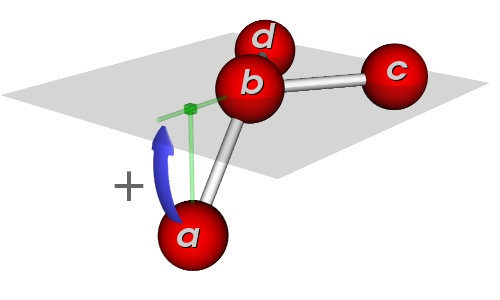
\includegraphics[width=7.5cm]{./Potentials/WilsonAnglePlus.jpg}
  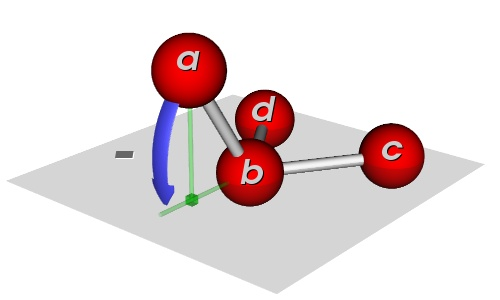
\includegraphics[width=7.5cm]{./Potentials/WilsonAngleMinus.jpg}
  \caption{The definition of the Wilson inversion-bend angle $\chi$.
  On the left a positive Wilson angle, and on the right a negative Wilson angle.}
  \label{Fig: Wilson definition}
\end{figure}

Common planar molecule that contain a double bond or sp$^2$ hybridization form planar groups with trigonal centers.
For example: the carbon and nitrogen centers in formamide, and the carbon centers in benzene.
The mode of motion is different from bond stretching, bending, and internal rotation.
The associated harmonic potential is
\begin{equation}
  U=\frac{1}{2} k \left(\chi\right)^2
\end{equation}
with $\chi$ the out-of-plane angle. Two possible definitions are in use
\begin{enumerate}
\item{the distance of the central atom from the plane defined by the other three atoms (pyramid height),}
\item{the average angle between any bond that extends from the central atom and the plane defined by the
other two bonds}.
\end{enumerate}
Note that an alternative to the out-of-plane angle is the \emph{improper torsion} using
\begin{equation}
  U=\frac{1}{2} k \left(1-\cos 2\chi\right)
\end{equation}
The out-of-plane potential can also be used for non-planar structure, for example in united-atom for chiral
centers to avoid inversion of the chiral center. Another example of its use is coordination complexes
where now the plane of the ligands need no longer be defined exactly.
In square planar complexes it is necessary to define an average plane through the ligands
(usually the least-square plane).
Note that the definition include one central atom
which is listed as the second in $a-b-c-d$: $a$, $c$, and $d$ are bonded to the central atom $b$.
The inversion angle potential is the average of the three possible inversion angle terms.

\begin{itemize}
  \item{HARMONIC\_INVERSION}\\
 \begin{equation}
  U=\frac{1}{2}p_0\left(\chi_{ijk}-p_1\right)^2
  \end{equation}
  2 arguments: $p_0/k_B$ in units of K/rad$^2$ and $p_1$ in degrees.
  \item{HARMONIC\_COSINE\_INVERSION}\\
 \begin{equation}
  U=\frac{1}{2}p_0\left(\cos\left(\chi_{ijk}\right)-\cos\left(p_1\right)\right)^2
  \end{equation}
  2 arguments: $p_0/k_B$ in units of K and $p_1$ in degrees.
  \item{PLANAR\_INVERSION}\\
 \begin{equation}
  U=p_0\left(1-\cos\left(\chi\right)\right)
  \end{equation}
  1 argument: $p_0/k_B$ in units of K.
  \item{MM3\_INVERSION}\\
  \begin{equation}
  \begin{split}
  U=\frac{1}{2}p_0 \left(\chi-p_1\right)^2\Bigl(1-0.014\left(\chi-p_1\right)+
   5.6\times10^{-5}\left(\chi-p_1\right)^2&-7\times10^{-7}\left(\chi-p_1\right)^3\\
   &+2.2\times10^{-8}\left(\chi-p_1\right)^4
   \Bigr)
  \end{split}
  \end{equation}
  2 arguments: $p_0$ in units of mdyne\,\AA/rad$^2$, $p_1$ in degrees.

  \item{FIXED\_INVERSION\_BEND}\\
   Use for inversion bend-angle constraint using the `SHAKE' and `RATTLE'-algorithm. 
   Applies to Molecular Dynamics and minimization. Does not work (yet) in Monte-Carlo.
\end{itemize}

\begin{figure}[t]
  \centering
  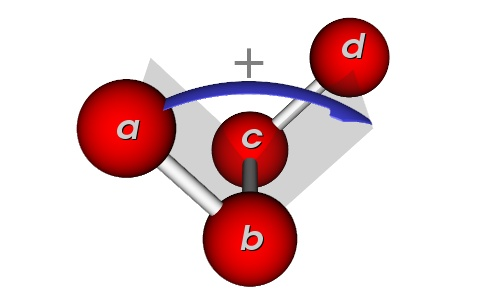
\includegraphics[width=7.5cm]{./Potentials/TorsionAnglePlus.jpg}
  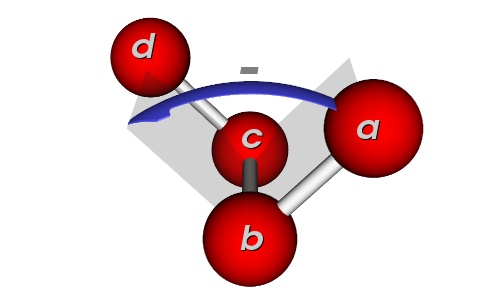
\includegraphics[width=7.5cm]{./Potentials/TorsionAngleMinus.jpg}
  \caption{The definition of the dihedral angle $\phi$: the angle between the planes formed by atoms a-b-c and b-c-d.
   On the left a positive dihedral angle, and on the right a negative dihedral angle.}
  \label{Fig: Torsion definition}
\end{figure}

\subsection{Torsion potential}

Intramolecular rotations about bonds do not occur freely. A possible description with a physical interpretation
is the three-term Fourier expansion
\begin{equation}
U=\frac{V_1}{2}\left[1+\cos\phi\right]+
  \frac{V_2}{2}\left[1-\cos2\phi\right]+
  \frac{V_3}{2}\left[1+\cos3\phi\right]
\end{equation}
\begin{enumerate}
\item{the 1 fold-term has been attributed to residual dipole-dipole interactions, to Van der Waal interactions,
or to any other direct interaction between atoms not accounted for otherwise,}
\item{the 2-fold arises from conjugation or hyper conjugation, being geometrically related to p orbitals,}
\item{and the 3-fold term has a steric (or bonding/anti-bonding) origin.}
\end{enumerate}
The values for 4-fold or higher are small and it is not known whether these are essential to include.
It may be that Van der Waals and dipole interactions already take care of these effects.
Torsions are even softer than bond angles. All possible values can be found in structures. Therefore, the
energy function must be valid over the entire range, the function must be periodic, and for reasons of
symmetry have stationary points at 0 and 180 degrees. The periodicity is the number of minima for the
potential, usually 3 for an sp$^3$-sp$^3$ bond and 2 for a conjugate bond.

The definition of a torsion includes two central and two terminal atoms. The term `torsional' means
an internal rigid rotation and `dihedral' means a rotation of two vicinal bonds about a middle bond.
\begin{itemize}
  \item{HARMONIC\_DIHEDRAL}\\
  \begin{equation}
  U=\frac{1}{2}p_0\left(\phi_{ijkl}-p_1\right)^2
  \end{equation}
  2 arguments: $p_0/k_B$ in units of K/rad$^2$, $p_1$ in degrees.

  \item{HARMONIC\_COSINE\_DIHEDRAL}\\
  \begin{equation}
  U=\frac{1}{2}p_0\left[\cos\left(\phi_{ijkl}\right)-\cos\left(p_1\right)\right]^2
  \end{equation}
  2 arguments: $p_0/k_B$ in units of K, $p_1$ in degrees.

  \item{THREE\_COSINE\_DIHEDRAL}\\
  \begin{equation}
  U=\frac{1}{2}p_0\left[1+\cos\left(\phi_{ijkl}\right)\right]+
    \frac{1}{2}p_1\left[1-\cos\left(2\phi_{ijkl}\right)\right]+
    \frac{1}{2}p_2\left[1+\cos\left(3\phi_{ijkl}\right)\right]
  \end{equation}
  3 arguments: $p_0/k_B,p_1/k_B,p_2/k_B$ in units of K


  \item{MM3\_DIHEDRAL}\\
  \begin{equation}
  U=\frac{1}{2}p_0\left[1+\cos\left(\phi_{ijkl}\right)\right]+
    \frac{1}{2}p_1\left[1-\cos\left(2\phi_{ijkl}\right)\right]+
    \frac{1}{2}p_2\left[1+\cos\left(3\phi_{ijkl}\right)\right]
  \end{equation}
  3 arguments: $p_0,p_1,p_2$ in units of kcal/mol.

  \item{CFF\_DIHEDRAL}\\
  \begin{equation}
  U=p_0\left[1-\cos\left(\phi_{ijkl}\right)\right]+
    p_1\left[1-\cos\left(2\phi_{ijkl}\right)\right]+
    p_2\left[1-\cos\left(3\phi_{ijkl}\right)\right]
  \end{equation}
  3 arguments: $p_0/k_B,p_1/k_B,p_2/k_B$ in units of K.

  \item{CFF\_DIHEDRAL2}\\
  \begin{equation}
  U=p_0\left[1+\cos\left(\phi_{ijkl}\right)\right]+
    p_1\left[1+\cos\left(2\phi_{ijkl}\right)\right]+
    p_2\left[1+\cos\left(3\phi_{ijkl}\right)\right]
  \end{equation}
  3 arguments: $p_0/k_B,p_1/k_B,p_2/k_B$ in units of K.

  \item{SIX\_COSINE\_DIHEDRAL}\\
  The Ryckaert-Bellemans potentials is often used for alkanes, the use implies exclusion of VDW-interactions
  between the first and last atoms of the dihedral, and $\phi'=\phi-\pi$ is defined according to the
  polymer convention $\phi'(trans)=0$.
  \begin{align}
  U=&\sum_{n=0}^5 p_n \cos^n\left(\phi'_{ijkl}\right)\\
    =&p_0+p_1\cos\left(\phi'_{ijkl}\right)+p_2\cos^2\left(\phi'_{ijkl}\right)+p_3\cos^3\left(\phi'_{ijkl}\right)
    p_4\cos^4\left(\phi'_{ijkl}\right)+p_5\cos^5\left(\phi'_{ijkl}\right)
  \end{align}
  6 arguments: $p_0/k_B,\dots,p_5/k_B$ in units of K.
  Rewritten in terms of $\phi$ the potential reads
  \begin{equation}
  U=p_0-p_1\cos\left(\phi_{ijkl}\right)+p_2\cos^2\left(\phi_{ijkl}\right)
    -p_3\cos^3\left(\phi_{ijkl}\right)+p_4\cos^4\left(\phi_{ijkl}\right)
    -p_5\cos^5\left(\phi_{ijkl}\right)
  \end{equation}

  \item{TRAPPE\_DIHEDRAL}\\
  \begin{equation}
  U=p_0+p_1\left[1+\cos\left(\phi_{ijkl}\right)\right]+
        p_2\left[1-\cos\left(2\phi_{ijkl}\right)\right]+
        p_3\left[1+\cos\left(3\phi_{ijkl}\right)\right]
  \end{equation}
  4 arguments: $p_0/k_B,p_1/k_B,p_2/k_B,p_3/k_B$ in units of K.

  \item{CVFF\_DIHEDRAL}\\
  \begin{equation}
  U=p_0\left[1+\cos\left(p_1\phi_{ijkl}-p_2\right)\right]
  \end{equation}
  3 arguments: $p_0/k_B$ in units of K, $p_1$ dimensionless, and $p_2$ in degrees.

  \item{OPLS\_DIHEDRAL}\\
  \begin{equation}
  U= \frac{1}{2}p_0+
    \frac{1}{2}p_1\left[1+\cos\left(\phi_{ijkl}\right)\right]+
    \frac{1}{2}p_2\left[1-\cos\left(2\phi_{ijkl}\right)\right]+
    \frac{1}{2}p_3\left[1+\cos\left(3\phi_{ijkl}\right)\right]
  \end{equation}
  4 arguments: $p_0/k_B,p_1/k_B,p_2/k_B,p_3/k_B$ in units of K.

  \item{FOURIER\_SERIES\_DIHEDRAL}\\
  The general form of a Fourier expansion is:
  \begin{equation}
  U=\sum_{n=1}^6\left[a_n\cos\left(n\phi\right)+b_n\sin\left(n\phi\right)\right]
  \end{equation}
  This form uses equilibrium angles of 0 for $n=1,3,5$ and 180 for $n=2,4,6$
  \begin{equation}
  \begin{split}
  U=&\frac{1}{2}p_0\left[1+\cos\phi\right]+
    \frac{1}{2}p_1\left[1-\cos\left(2\phi\right)\right]+
    \frac{1}{2}p_2\left[1+\cos\left(3\phi\right)\right]+\\
    &\frac{1}{2}p_3\left[1-\cos\left(4\phi\right)\right]+
    \frac{1}{2}p_4\left[1+\cos\left(5\phi\right)\right]+
    \frac{1}{2}p_5\left[1-\cos\left(6\phi\right)\right]
  \end{split}
  \end{equation}
  6 arguments: $p_0/k_B,p_1/k_B,p_2/k_B,p_3/k_B,p_4/k_B,p_5/k_B$ in units of K.

  \item{FOURIER\_SERIES\_DIHEDRAL\_2}\\
  The general form of a Fourier expansion is:
  \begin{equation}
  U=\sum_{n=1}^6\left[a_n\cos\left(n\phi\right)+b_n\sin\left(n\phi\right)\right]
  \end{equation}
  This form uses equilibrium angles of 0 for $n=1,3,4,5,6$ and 180 for $n=2$
  \begin{equation}
  \begin{split}
  U=&\frac{1}{2}p_0\left[1+\cos\phi\right]+
    \frac{1}{2}p_1\left[1-\cos\left(2\phi\right)\right]+
    \frac{1}{2}p_2\left[1+\cos\left(3\phi\right)\right]+\\
    &\frac{1}{2}p_3\left[1+\cos\left(4\phi\right)\right]+
    \frac{1}{2}p_4\left[1+\cos\left(5\phi\right)\right]+
    \frac{1}{2}p_5\left[1+\cos\left(6\phi\right)\right]
  \end{split}
  \end{equation}
  6 arguments: $p_0/k_B,p_1/k_B,p_2/k_B,p_3/k_B,p_4/k_B,p_5/k_B$ in units of K.

  \item{FIXED\_DIHEDRAL}\\
   Use for dihedral-angle constraint using the `SHAKE' and `RATTLE'-algorithm. 
   Applies to Molecular Dynamics and minimization. Does not work (yet) in Monte-Carlo.
\end{itemize}

\begin{center}
\shadowbox{
\begin{minipage}{16cm}
\begin{quote}
The following identities are convenient when dealing with torsions:
\begin{equation}
\begin{split}
\cos 1x &= \cos x\\
\cos 2x &= -1+2\cos^2 x\\
\cos 3x &= -3\cos x+4\cos^3x\\
\cos 4x &= 1-8\cos^2x+8\cos^4x\\
\cos 5x &= 5\cos x-20\cos^3x+16\cos^5x\\
\cos 6x &= -1+18\cos^2 x-48\cos^4 x+32\cos^6x
\end{split}
\end{equation}

\begin{equation}
\begin{split}
\sin 1x &= \sin x\\
\sin 2x &= (\sin x) (2\cos x)\\
\sin 3x &= (\sin x) (-1+4\cos^2 x)\\
\sin 4x &= (\sin x ) (-4\cos x +8\cos^3x)\\
\sin 5x &= (\sin x) (1-12\cos^2x+16\cos^4x)\\
\sin 6x &= (\sin x) (6\cos x-32\cos^3x+32\cos^5x)
\end{split}
\end{equation}
\end{quote}
\end{minipage}}
\end{center}

\subsection{Improper torsion potential}

\begin{figure}[t]
  \centering
  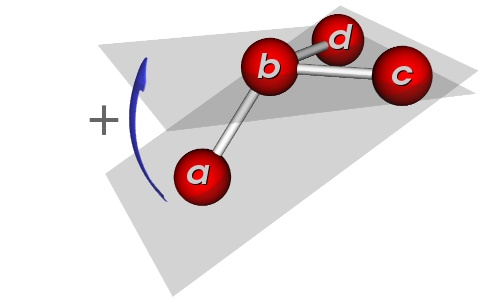
\includegraphics[width=7.5cm]{./Potentials/ImproperTorsionAnglePlus.jpg}
  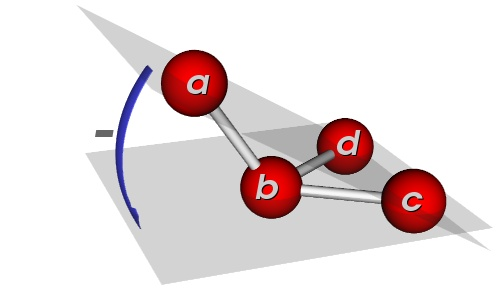
\includegraphics[width=7.5cm]{./Potentials/ImproperTorsionAngleMinus.jpg}
  \caption{The most common (CVFF, DLPOLY) definition of the improper dihedral angle 
   $\phi$: the angle between the planes formed by atoms `a-c-d' and `c-d-b'.
   On the left a positive improper dihedral angle, and on the right a negative improper dihedral angle.
   The atoms need to be listed in the order `a-c-d-b'. Note that an exchange of atoms `c' and `d' leads to a change
   of sign, but \emph{not} in magntitude.}
  \label{Fig: Improper Torsion definition}
  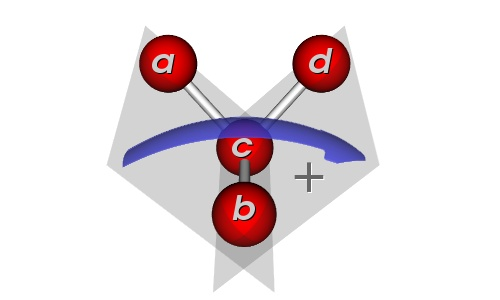
\includegraphics[width=7.5cm]{./Potentials/ImproperTorsionAngleTypeA.jpg}
  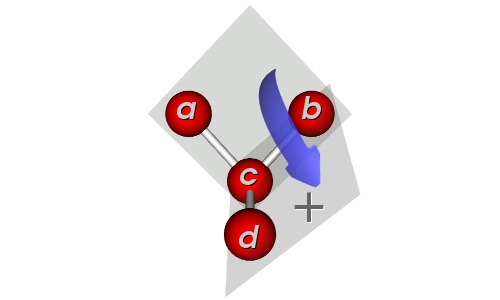
\includegraphics[width=7.5cm]{./Potentials/ImproperTorsionAngleTypeB.jpg}
  \caption{A second definition of the improper dihedral angle (CHARMM, AMBER). The central atom is `c', and the improper torsion
   is enter as `a-b-c-d'. Howevere, an exchange of terminal atoms leads to a change in magntitude and the improper torsion
   needs to be symmetrized by adding two additional improper torsions `b-d-c-a' and `d-a-c-b' and rescaling the force constant
   by a factor of $1/3$.}
\end{figure}

The improper torsion is an alternative for the out-of-plane angle, and a possible definition is
\begin{equation}
  U=\frac{1}{2} k \left(1-\cos 2\chi\right)
\end{equation}
It is termed `improper torsion' because it simply treats the four atoms in the plane as if they were
bonded in the same way as in a true torsional angle. Note that the definition include one central atom
which is listed as the second in $a-b-c-d$: $a$, $c$, and $d$ are bonded to the central atom $b$.
Improper torsions are often used to keep sp2 atoms planar and sp3 atoms in a tetrahedral geometry.

The CHARMM convention is to list the central atom first, while there are no rules how to order the other three atoms.
Hence, six possibilities exist for the definition of an improper torsion. The AMBER convention is that the out-of-plane
atom is listed in the third position and the order of the other atoms is determined alphabetically by atom type, and
by the atom number (i.e. the order in the molecule) when atom types are identical.

\begin{itemize}
  \item{HARMONIC\_IMPROPER\_DIHEDRAL}\\
  \begin{equation}
  U=\frac{1}{2}p_0\left(\phi_{ijkl}-p_1\right)^2
  \end{equation}
  2 arguments: $p_0/k_B$ in units of K/rad$^2$, $p_1$ in degrees.

  \item{HARMONIC\_COSINE\_IMPROPER\_DIHEDRAL}\\
  \begin{equation}
  U=\frac{1}{2}p_0\left[\cos\left(\phi_{ijkl}\right)-\cos\left(p_1\right)\right]^2
  \end{equation}
  2 arguments: $p_0/k_B$ in units of K, $p_1$ in degrees.

  \item{THREE\_COSINE\_IMPROPER\_DIHEDRAL}\\
  \begin{equation}
  U=\frac{1}{2}p_0\left[1+\cos\left(\phi_{ijkl}\right)\right]+
    \frac{1}{2}p_1\left[1-\cos\left(2\phi_{ijkl}\right)\right]+
    \frac{1}{2}p_2\left[1+\cos\left(3\phi_{ijkl}\right)\right]
  \end{equation}
  3 arguments: $p_0/k_B,p_1/k_B,p_2/k_B$ in units of K.

  \item{MM3\_IMPROPER\_DIHEDRAL}\\
  \begin{equation}
  U=\frac{1}{2}p_0\left[1+\cos\left(\phi_{ijkl}\right)\right]+
    \frac{1}{2}p_1\left[1-\cos\left(2\phi_{ijkl}\right)\right]+
    \frac{1}{2}p_2\left[1+\cos\left(3\phi_{ijkl}\right)\right]
  \end{equation}
  3 arguments: $p_0,p_1,p_2$ in units of kcal/mol.


  \item{CFF\_IMPROPER\_DIHEDRAL}\\
  \begin{equation}
  U=p_0\left[1-\cos\left(\phi_{ijkl}\right)\right]+
    p_1\left[1-\cos\left(2\phi_{ijkl}\right)\right]+
    p_2\left[1-\cos\left(3\phi_{ijkl}\right)\right]
  \end{equation}
  3 arguments: $p_0/k_B,p_1/k_B,p_2/k_B$ in units of K.

  \item{CFF\_IMPROPER\_DIHEDRAL2}\\
  \begin{equation}
  U=p_0\left[1+\cos\left(\phi_{ijkl}\right)\right]+
    p_1\left[1+\cos\left(2\phi_{ijkl}\right)\right]+
    p_2\left[1+\cos\left(3\phi_{ijkl}\right)\right]
  \end{equation}
  3 arguments: $p_0/k_B,p_1/k_B,p_2/k_B$ in units of K.

  \item{SIX\_COSINE\_IMPROPER\_DIHEDRAL}\\
  The Ryckaert-Bellemans potentials is often used for alkanes, the use implies exclusion of VDW-interactions
  between the first and last atoms of the dihedral, and $\phi'=\phi-\pi$ is defined according to the
  polymer convention $\phi'(trans)=0$.
  \begin{align}
  U=&\sum_{n=0}^5 p_n \cos^n\left(\phi'_{ijkl}\right)\\
    =&p_0+p_1\cos\left(\phi'_{ijkl}\right)+p_2\cos^2\left(\phi'_{ijkl}\right)+p_3\cos^3\left(\phi'_{ijkl}\right)
    p_4\cos^4\left(\phi'_{ijkl}\right)+p_5\cos^5\left(\phi'_{ijkl}\right)
  \end{align}
  6 arguments: $p_0/k_B,\dots,p_5/k_B$ in units of K.
  Rewritten in terms of $\phi$ the potential reads
  \begin{equation}
  U=p_0-p_1\cos\left(\phi_{ijkl}\right)+p_2\cos^2\left(\phi_{ijkl}\right)
    -p_3\cos^3\left(\phi_{ijkl}\right)+p_4\cos^4\left(\phi_{ijkl}\right)
    -p_5\cos^5\left(\phi_{ijkl}\right)
  \end{equation}

  \item{TRAPPE\_IMPROPER\_DIHEDRAL}\\
  \begin{equation}
  U=p_0+p_1\left[1+\cos\left(\phi_{ijkl}\right)\right]+
        p_2\left[1-\cos\left(2\phi_{ijkl}\right)\right]+
        p_3\left[1+\cos\left(3\phi_{ijkl}\right)\right]
  \end{equation}
  4 arguments: $p_0/k_B,p_1/k_B,p_2/k_B,p_3/k_B$ in units of K.

  \item{CVFF\_IMPROPER\_DIHEDRAL}\\
  \begin{equation}
  U=p_0\left[1+\cos\left(p_1\phi_{ijkl}-p_2\right)\right]
  \end{equation}
  3 arguments: $p_0/k_B$ in units of K, $p_1$ dimensionless, and $p_2$ in degrees.

  \item{OPLS\_IMPROPER\_DIHEDRAL}\\
  \begin{equation}
  U= \frac{1}{2}p_0+
    \frac{1}{2}p_1\left[1+\cos\left(\phi_{ijkl}\right)\right]+
    \frac{1}{2}p_2\left[1-\cos\left(2\phi_{ijkl}\right)\right]+
    \frac{1}{2}p_3\left[1+\cos\left(3\phi_{ijkl}\right)\right]
  \end{equation}
  4 arguments: $p_0/k_B,p_1/k_B,p_2/k_B,p_3/k_B$ in units of K.

  \item{FOURIER\_SERIES\_IMPROPER\_DIHEDRAL}\\
  The general form of a Fourier expansion is:
  \begin{equation}
  U=\sum_{n=1}^6\left[a_n\cos\left(n\phi\right)+b_n\sin\left(n\phi\right)\right]
  \end{equation}
  This form uses equilibrium angles of 0 for $n=1,3,5$ and 180 for $n=2,4,6$
  \begin{equation}
  \begin{split}
  U=&\frac{1}{2}p_0\left[1+\cos\phi\right]+
    \frac{1}{2}p_1\left[1-\cos\left(2\phi\right)\right]+
    \frac{1}{2}p_2\left[1+\cos\left(3\phi\right)\right]+\\
    &\frac{1}{2}p_3\left[1-\cos\left(4\phi\right)\right]+
    \frac{1}{2}p_4\left[1+\cos\left(5\phi\right)\right]+
    \frac{1}{2}p_5\left[1-\cos\left(6\phi\right)\right]
  \end{split}
  \end{equation}
  6 arguments: $p_0/k_B,p_1/k_B,p_2/k_B,p_3/k_B,p_4/k_B,p_5/k_B$ in units of K.

  \item{FOURIER\_SERIES\_IMPROPER\_DIHEDRAL\_2}\\  The general form of a Fourier expansion is:
  \begin{equation}
  U=\sum_{n=1}^6\left[a_n\cos\left(n\phi\right)+b_n\sin\left(n\phi\right)\right]
  \end{equation}
  This form uses equilibrium angles of 0 for $n=1,3,4,5,6$ and 180 for $n=2$
  \begin{equation}
  \begin{split}
  U=&\frac{1}{2}p_0\left[1+\cos\phi\right]+
    \frac{1}{2}p_1\left[1-\cos\left(2\phi\right)\right]+
    \frac{1}{2}p_2\left[1+\cos\left(3\phi\right)\right]+\\
    &\frac{1}{2}p_3\left[1+\cos\left(4\phi\right)\right]+
    \frac{1}{2}p_4\left[1+\cos\left(5\phi\right)\right]+
    \frac{1}{2}p_5\left[1+\cos\left(6\phi\right)\right]
  \end{split}
  \end{equation}
  6 arguments: $p_0/k_B,p_1/k_B,p_2/k_B,p_3/k_B,p_4/k_B,p_5/k_B$ in units of K.
  \item{FIXED\_IMPROPER\_DIHEDRAL}\\
   Use for improper-dihedral-angle constraint using the `SHAKE' and `RATTLE'-algorithm.      
   Applies to Molecular Dynamics and minimization. Does not work (yet) in Monte-Carlo.

\end{itemize}


\section{Non-bonded potentials}

\subsection{Van der Waals potentials}

The general expression for Van der Waals potentials when using a cutoff distance is
\begin{equation}
 U_{ij}^{\text{VDW}}=\begin{cases}
    U_{ij}\left(r_{ij}\right)& \text{if }r_{ij}\leq r_c\\
    0 & \text{otherwise}
   \end{cases}
\end{equation}

\begin{itemize}

  \item{NONE}\\
  \begin{equation}
    U=0
  \end{equation}
  zero parameters.
\item{$\begin{array}{l}\text{LENNARD\_JONES}\\
      \text{LENNARD\_JONES\_SMOOTHED3}\\
      \text{LENNARD\_JONES\_SMOOTHED5}\end{array}$}\\
  \begin{equation}
    U= 
      4 p_0 \left[\left(\frac{p_1}{r}\right)^{12}-\left(\frac{p_1}{r}\right)^6\right]
  \end{equation}
  2 parameters: $p_0/k_B$ in units of K, and $p_1$ in \AA.
\item{$\begin{array}{l}\text{FEYNMAN\_HIBBS\_LENNARD\_JONES}\\
      \text{FEYNMAN\_HIBBS\_LENNARD\_JONES\_SMOOTHED3}\\
      \text{FEYNMAN\_HIBBS\_LENNARD\_JONES\_SMOOTHED5}\end{array}$}\\
  \begin{equation}
    U=4 p_0 \left[\left(\frac{p_1}{r}\right)^{12}-\left(\frac{p_1}{r}\right)^6\right]
      +\frac{\hbar^2}{24 p_2 k_B T} 4 p_0\left[132\left(\frac{p_1}{r}\right)^{12}-30\left(\frac{p_1}{r}\right)^6\right]\frac{1}{r^2}
  \end{equation}
  3 parameters: $p_0/k_B$ in units of K, $p_1$ in \AA, and $p_2$ is the reduced mass in unified atomic mass units.

\item{$\begin{array}{l}\text{FEYNMAN\_HIBBS2\_LENNARD\_JONES}\\
      \text{FEYNMAN\_HIBBS\_LENNARD\_JONES2\_SMOOTHED3}\\
      \text{FEYNMAN\_HIBBS\_LENNARD\_JONES2\_SMOOTHED5}\end{array}$}\\
  \begin{equation}
    U=4 p_0 \left[\left(\frac{p_1}{r}\right)^{12}-\left(\frac{p_1}{r}\right)^6\right]
      +4 p_0\left[132\left(\frac{p_1}{r}\right)^{12}-30\left(\frac{p_1}{r}\right)^6\right]\frac{p_2}{r^2}
  \end{equation}
  3 parameters: $p_0/k_B$ in units of K, $p_1$ in \AA, and $p_2$ in units of $\AA^2$.

  \item{LENNARD\_JONES\_SHIFTED\_FORCE}\\
  \begin{equation}
       U=4 p_0 \left\{\left[\left(\frac{p_1}{r}\right)^{12}-\left(\frac{p_1}{r}\right)^6\right]-
           \left[\left(\frac{p_1}{r_c}\right)^{12}-\left(\frac{p_1}{r_c}\right)^6\right]+
           \left[12\left(\frac{p_1}{r_c}\right)^{12}-6\left(\frac{p_1}{r_c}\right)^{6}\right]\frac{\left(r-r_c\right)}{r_c}\right\}
  \end{equation}
  2 parameters: $p_0/k_B$ in units of K, and $p_1$ in \AA.

  \item{LENNARD\_JONES\_SHIFTED\_FORCE2}\\
  \begin{equation}
       4 p_0 \left\{\left[\left(\frac{p_1}{r}\right)^{12}-\left(\frac{p_1}{r}\right)^6\right]
       +\left[6\left(\frac{p_1}{r_c}\right)^{12}-3\left(\frac{p_1}{r_c}\right)^6\right]\frac{r^2}{r_c^2}
       +7\left(\frac{p_1}{r_c}\right)^{12}+4\left(\frac{p_1}{r_c}\right)^6\right\}
  \end{equation}
  2 parameters: $p_0/k_B$ in units of K, and $p_1$ in \AA.

\item{$\begin{array}{l}\text{POTENTIAL\_12\_6}\\
      \text{POTENTIAL\_12\_6\_SMOOTHED3}\\
      \text{POTENTIAL\_12\_6\_SMOOTHED5}\end{array}$}\\
  \begin{equation}
    U= 
      \frac{p_0}{r^{12}}-\frac{p_1}{r^6}
  \end{equation}
   2 parameters: $p_0/k_B$ in units of K\,\AA$^{12}$, and $p_1/k_B$ in units of K\,\AA$^6$.

\item{$\begin{array}{l}\text{POTENTIAL\_12\_6\_2\_0}\\
      \text{POTENTIAL\_12\_6\_2\_0\_SMOOTHED3}\\
      \text{POTENTIAL\_12\_6\_2\_0\_SMOOTHED5}\end{array}$}\\
  \begin{equation}
    U= 
      \frac{p_0}{r^{12}}+\frac{p_1}{r^6}+\frac{p_2}{r^2}+p_3
  \end{equation}
   4 parameters: $p_0/k_B$ in units of K\,\AA$^{12}$, $p_1/k_B$ in units of K\,\AA$^6$, $p_2/k_B$ in units of K\,\AA$^2$, 
   and $p_3$ in units of K.

\item{$\begin{array}{l}\text{MORSE}\\
      \text{MORSE\_SMOOTHED3}\\
      \text{MORSE\_SMOOTHED5}\end{array}$}\\
  \begin{equation}
    U= p_0 \left[(1-{e^{-p_1*(r-p_2)}})^2-1\right]
  \end{equation}
   3 parameters: $p_0/k_B$ in units of K, $p_1$ in units of $\AA^{-1}$ and $p_2$ in units of \AA.

\item{$\begin{array}{l}\text{MORSE2}\\
      \text{MORSE2\_SMOOTHED3}\\
      \text{MORSE2\_SMOOTHED5}\end{array}$}\\
  \begin{equation}
    U= p_0 \left[e^{p_1*(1-r/p_2)}-2e^{(p_1/2)*(1-r/p_2)}\right]
  \end{equation}
   3 parameters: $p_0/k_B$ in units of K, $p_1$ in units of $\AA^{-1}$ and $p_2$ in units of \AA.

\item{$\begin{array}{l}\text{MORSE3}\\
      \text{MORSE3\_SMOOTHED3}\\
      \text{MORSE3\_SMOOTHED5}\end{array}$}\\
  \begin{equation}
    U= p_0 \left[\left(1-e^{\left(\frac{-\ln{2}}{2^{\nicefrac{1}{6}}-1}\right)\left(\frac{r}{p_2}-2^{\nicefrac{1}{6}}\right)}\right)^2-1\right]
  \end{equation}
   2 parameters: $p_0/k_B$ in units of K $p_2$ in units of \AA. This form of the Morse potential resembles the Lennard-Jones potential.

\item{$\begin{array}{l}\text{CFF\_9\_6}\\
      \text{CFF\_9\_6\_SMOOTHED3}\\
      \text{CFF\_9\_6\_SMOOTHED5}\end{array}$}\\
  \begin{equation}
    U= 
      \frac{p_0}{r^{9}}-\frac{p_1}{r^6}
  \end{equation}
   2 parameters: $p_0/k_B$ in units of K\,\AA$^{9}$, and $p_1/k_B$ in units of K\,\AA$^6$.

\item{$\begin{array}{l}\text{CFF\_EPS\_SIGMA}\\
      \text{CFF\_EPS\_SIGMA\_SMOOTHED3}\\
      \text{CFF\_EPS\_SIGMA\_SMOOTHED5}\end{array}$}\\
  \begin{equation}
    U_{ij}= 
      p_0 \left[2\left(\frac{p_1}{r}\right)^{9}-3\left(\frac{p_1}{r}\right)^6\right]
  \end{equation}
  2 parameters: $p_0/k_B$ in units of K, and $p_1$ in \AA.

\item{$\begin{array}{l}\text{BUCKINGHAM}\\
      \text{BUCKINGHAM\_SMOOTHED3}\\
      \text{BUCKINGHAM\_SMOOTHED5}\end{array}$}\\
  \begin{equation}
  U=
     p_0 e^{-p_1 r}-\frac{p_2}{r^{6}}
  \end{equation}
  3 parameters: $p_0/k_B$ in units of K, $p_1$ in units of \AA$^{-1}$, and $p_2$ in K\,\AA$^6$. Warning: in literature sometimes $\rho=\frac{1}{p_1}$ is given,
  $\rho$ is usually around 0.3-0.4 \AA, $p_1$ is usually around 2-4 \AA$^{-1}$.

\item{$\begin{array}{l}\text{BUCKINGHAM2}\\
      \text{BUCKINGHAM2\_SMOOTHED3}\\
      \text{BUCKINGHAM2\_SMOOTHED5}\end{array}$}\\
  \begin{equation}
  U=\begin{cases}
     10^{10}  & r<p_3\\
     p_0 e^{-p_1 r}-\frac{p_2}{r^{6}} & \text{otherwise}
    \end{cases}
  \end{equation}
  4 parameters: $p_0/k_B$ in units of K, $p_1$ in units of \AA$^{-1}$, $p_2$ in K\,\AA$^6$, and $p_3$ in [\AA].
  Warning: in literature sometimes $\rho=\frac{1}{p_1}$ is given,
  $\rho$ is usually around 0.3-0.4 \AA, $p_1$ is usually around 2-4 \AA$^{-1}$.

\item{$\begin{array}{l}\text{MM3\_VDW}\\
      \text{MM3\_VDW\_SMOOTHED3}\\
      \text{MM3\_VDW\_SMOOTHED5}\end{array}$}\\
  \begin{equation}
    U_{ij}= \begin{cases}
       \sqrt{p_0^i p_0^j}\left[1.84\times10^5 e^{-\frac{12}{P}}-2.25\,P^6\right] & \text{if }P\geq 3.02\\
       \sqrt{p_0^i p_0^j} 192.27 P^2  & \text{if }P<3.02
       \end{cases}
  \end{equation}
  with $P=\frac{p_1^i+p_1^j}{r_{ij}}$ and where $p_1^i$ and $p_1^j$ are the VDW radii of atoms $i$ and $j$,
  and $r_{ij}$ the separation distance in \AA\ between atoms $i$ and $j$. \\
  2 arguments: $p_0$ in units of kcal/mol, $p_1$ in units of \AA.

\item{$\begin{array}{l}\text{MATSUOKA\_CLEMENTI\_YOSHIMINE}\\
      \text{MATSUOKA\_CLEMENTI\_YOSHIMINE\_SMOOTHED3}\\
      \text{MATSUOKA\_CLEMENTI\_YOSHIMINE\_SMOOTHED5}\end{array}$}\\
  \begin{equation}
    U= p_0e^{-p_1 r_{ij}}+p_2e^{-p_3 r_{ij}}
  \end{equation}
   4 arguments: $p_0/k_B$ in units of K, $p_1$ in units of \AA$^{-1}$, $p_2/k_B$ in units of K, and $p_3$ in units of \AA$^{-1}$.

\item{$\begin{array}{l}\text{GENERIC}\\
      \text{GENERIC\_SMOOTHED3}\\
      \text{GENERIC\_SMOOTHED5}\end{array}$}\\
  \begin{equation}
    U= p_0 e^{-p_1 r}-\frac{p_2}{r^4}-\frac{p_3}{r^6}-\frac{p_4}{r^8}-\frac{p_5}{r^{10}}
  \end{equation}
  6 arguments: $p_0/k_B$ in units of K, $p_1$ in units of \AA$^{-1}$, $p_2/k_B$ in units of K\,\AA$^{4}$, $p_3/k_B$ in units of K\,\AA$^{6}$,
  $p_4/k_B$ in units of K\,\AA$^{8}$, and $p_5/k_B$ in units of K\,\AA$^{10}$.

\item{$\begin{array}{l}\text{PELLENQ\_NICHOLSON}\\
      \text{PELLENQ\_NICHOLSON\_SMOOTHED3}\\
      \text{PELLENQ\_NICHOLSON\_SMOOTHED5}\end{array}$}\\
  \begin{equation}
    U= p_0 e^{-p_1 r}-f_6 \frac{p_2}{r^6}-f_8\frac{p_3}{r^8}-f_{10}\frac{p_4}{r^{10}}
  \end{equation}
  with
  \begin{equation}
   f_{2n}=1-\sum_{k=0}^{2n}\frac{\left(p_1 r_{ij}\right)^k}{k!} e^{-p_1 r_{ij}}
  \end{equation}
  5 arguments: $p_0/k_B$ in units of K, $p_1$ in units of \AA$^{-1}$, $p_2/k_B$ in units of K\,\AA$^{6}$,
  $p_3/k_B$ in units of K\,\AA$^{8}$, and $p_4/k_B$ in units of K\,\AA$^{10}$.

\item{$\begin{array}{l}\text{HYDRATED\_ION\_WATER}\\
      \text{HYDRATED\_ION\_WATER\_SMOOTHED3}\\
      \text{HYDRATED\_ION\_WATER\_SMOOTHED5}\end{array}$}\\
  \begin{equation}
    U= p_0 e^{-p_1 r}-\frac{p_2}{r^4}-\frac{p_3}{r^6}-\frac{p_4}{r^{12}}
  \end{equation}
  5 arguments: $p_0/k_B$ in units of K, $p_1$ in units of \AA$^{-1}$, $p_2/k_B$ in units of K\,\AA$^{4}$,
  $p_3/k_B$ in units of K\,\AA$^{6}$, and $p_4/k_B$ in units of K\,\AA$^{12}$.

\item{$\begin{array}{l}\text{MIE}\\
      \text{MIE\_SMOOTHED3}\\
      \text{MIE\_SMOOTHED5}\end{array}$}\\
The Mie-potential \cite{Mie1903}
  \begin{equation}
    U= 
      \left(\frac{p_0}{r^{p_1}}-\frac{p_2}{r^{p_3}}\right)
  \end{equation}
   4 arguments: $p_0/k_B$ in units of K \AA$^{p_1}$, $p_1$ dimensionless,
  $p_2/k_B$ in units of K \AA$^{p_3}$, and $p_3$ dimensionless.

\item{$\begin{array}{l}\text{BORN\_HUGGINS\_MEYER}\\
      \text{BORN\_HUGGINS\_MEYER\_SMOOTHED3}\\
      \text{BORN\_HUGGINS\_MEYER\_SMOOTHED5}\end{array}$}\\
  \begin{equation}
    U_{ij}=p_0 e^{p_1\left(p_2-r_{ij}\right)}-\frac{p_3}{r_{ij}^6}-\frac{p_4}{r_{ij}^8}
  \end{equation}
  5 arguments: $p_0/k_B$ in units of K, $p_1$ dimensionless, $p_2$ in units of \AA, $p_3/k_B$ in units of K\,\AA$^{6}$, and
  $p_4/k_B$ in units of K\,\AA$^{8}$.

\item{$\begin{array}{l}\text{HYDROGEN}\\
      \text{HYDROGEN\_SMOOTHED3}\\
      \text{HYDROGEN\_SMOOTHED5}\end{array}$}\\
  \begin{equation}
    U= 
      \frac{p_0}{r^{12}}-\frac{p_1}{r^{10}}
  \end{equation}
   2 arguments: $p_0/k_B$ in units of K\,\AA$^{12}$, and $p_1/k_B$ in units of K\,\AA$^{10}$.

\end{itemize}

\subsection{Tail corrections}

\subsubsection*{energy}

\begin{equation}
 U^{\text{Tail}}=\frac{2 \pi}{V}\sum_a \sum_b N_a N_b \left[\int_{r_c}^\infty r^2 U\left(r\right)\, dr\right]
\end{equation}

\begin{tabular}{|l|l|}
\hline
potential & $\int_{r_c}^\infty r^2 U\left(r\right)$\\
\hline\hline
  LENNARD\_JONES &
      $\frac{4}{3}\,p_0\,p_1^3 \left[\frac{1}{3}\left(\frac{p_1}{r}\right)^{9}-\left(\frac{p_1}{r}\right)^3\right]$\\
  LENNARD\_JONES\_SHIFTED\_FORCE & -\\
\hline
\end{tabular}

\subsubsection*{pressure}
\begin{align}
 P^{\text{Tail}}=&-\sum_a \sum_b \frac{2\pi}{3V} N_a N_b \left[\int_{r_c}^\infty r^2\, r\frac{\partial U\left(r\right)}{\partial r}\, dr\right]\\
    =&\sum_a \sum_b\left(\frac{2\pi}{3V} r_c^3 N_a N_b U\left(r_c\right)+U^{\text{Tail}}\right)
\end{align}
\subsubsection*{chemical potential}
\begin{equation}
 \beta \mu^{\text{Tail}}=2 U^{\text{Tail}}
\end{equation}

\subsection{Electrostatics}

\subsubsection{Charge-charge interaction}
\begin{itemize}
\item{Ewald}\\
The potential energy for a system of charges in a periodic system can be written as
\begin{equation}
 U=U^{\text{real}}+U^{\text{rec}}
\end{equation}
where
\begin{equation}
 \begin{split}
 U^{\text{real}}
  &=\sum_{i<j} q_i q_j \frac{\text{erfc}\left(\alpha r_{ij}\right)}{r_{ij}}\\
 U^{\text{rec}}
  &=\frac{2\pi}{V}\sum_{\mathbf{k}\not=0}\frac{1}{k^2} e^{-\frac{k^2}{4\alpha^2}}
  \left(\left|\sum_{i=1}^N q_i\cos\left(\mathbf{k}\cdot\mathbf{r}_i\right)\right|^2+
   \left|\sum_{i=1}^N q_i\sin\left(\mathbf{k}\cdot\mathbf{r}_i\right)\right|^2\right)
 -\sum_i\frac{\alpha}{\sqrt{\pi}}q_i^2
 \end{split}
\end{equation}
where $q_i$ and $q_j$ are the charges of particle $i$ and $j$, respectively, $\mathbf{r}_i$ the position of atom $i$, $V$ the volume of the cell,
$\alpha$ a damping factor, $k$ the wavelength, and `erfc' the error function complement. The expression gives the \emph{exact} solution for charges
in a periodic system up to arbitrary precision. One part is computed in `real' space, and the long-range part is more conveniently computed in Fourier space.

\item{CoulombTruncated}
\begin{equation}
 U=\begin{cases}
    \sum_{i<j} \frac{1}{4\pi\epsilon}\frac{q_i q_j}{r_{ij}}& \text{if }r_{ij}\leq r_c\\
    0 & \text{otherwise}
   \end{cases}
\end{equation}

\item{CoulombShifted}
\begin{equation}
 U=\begin{cases}
    \sum_{i<j} \frac{q_i q_j}{4\pi \epsilon }\left(\frac{1}{r_{ij}}-\frac{1}{r_c}\right)& \text{if }r_{ij}\leq r_c\\
    0 & \text{otherwise}
   \end{cases}
\end{equation}

\item{CoulombSmoothed}
\item{Wolf}

\end{itemize}

\subsubsection{Charge-dipole interaction}

\begin{itemize}
\item{Ewald}\\
\item{CoulombTruncated}
\begin{equation}
 U=\begin{cases}
    \sum_{i,j} \frac{1}{4\pi\epsilon} \frac{-q_i}{r^2_{ij}}
      \left({\boldsymbol \mu}_j\cdot\mathbf{r}_{ij}\right)& \text{if }r_{ij}\leq r_c\\
    0 & \text{otherwise}
   \end{cases}
\end{equation}
\end{itemize}


\subsubsection{Dipole-dipole interaction}

\begin{itemize}
\item{Ewald}\\
\item{CoulombTruncated}
\begin{equation}
 U=\begin{cases}
    \sum_{i,j} \frac{1}{4\pi\epsilon}\frac{1}{r^3_{ij}}
    \left[{\boldsymbol \mu}_i\cdot {\boldsymbol \mu}_j-3\frac{\left({\boldsymbol\mu}_i\cdot\mathbf{r}_{ij}\right)
    \left(\mathbf{r}_{ij}\cdot{\boldsymbol \mu}_j\right)}{r^2_{ij}}\right]& \text{if }r_{ij}\leq r_c\\
    0 & \text{otherwise}
   \end{cases}
\end{equation}
\end{itemize}


\section{Bonded potentials cross terms}

\subsection{Bond-bond potential}

\begin{itemize}
  \item{CFF\_BOND\_BOND\_CROSS,CVFF\_BOND\_BOND\_CROSS}\\
  \begin{equation}
  U=p_0\left(r-p_1\right)\left(r'-p_2\right)
  \end{equation}
  3 arguments: $p_0/k_B$ in units of K/\AA$^2$, $p_0$ and $p_1$ in \AA.
\end{itemize}

\subsection{Bond-bend potential}

\begin{itemize}
  \item{CFF\_BOND\_BEND\_CROSS,CVFF\_BOND\_BEND\_CROSS}\\
  \begin{equation}
  U=\left(\theta-p_0\right)\left[p_1\left(r-p_2\right)+p_3\left(r'-p_4\right)\right]
  \end{equation}
  5 arguments: $p_0$ in degrees, $p_1/k_B$ in units of K/\AA/rad, $p_2$ in \AA, $p_3/k_B$ in units of K/\AA/rad, $p_4$ in \AA.

  \item{MM3\_BOND\_BEND\_CROSS}
  \begin{equation}
  U=p_0\left[\left(r-p_1\right)+\left(r'-p_2\right)\right]\left(\theta-p_3\right)
  \end{equation}
  4 arguments: $p_0$ in mdyne/rad, $p_1$ and $p_2$ in \AA, and $p_3$ in degrees.

  \item{TRUNCATED\_HARMONIC}
  \begin{equation}
  U=\frac{1}{2}p_0\left(\theta-p_1\right)^2 e^{-\frac{r_{ij}^8+r_{ik}^8}{p_2^8}}
  \end{equation}
  3 arguments: $p_0/k_B$ in K/rad$^2$, $p_1$ in degrees, and $p_2$ in units of \AA.

  \item{SCREENED\_HARMONIC}
  \begin{equation}
  U=\frac{1}{2}p_0\left(\theta-p_1\right)^2 e^{-\left(\frac{r_{ij}}{p_2}+\frac{r_{ik}}{p_3}\right)}
  \end{equation}
  4 arguments: $p_0$ in K/rad$^2$, $p_1$ in degrees, $p_2$ and $p_3$ in units of \AA.

  \item{SCREENED\_VESSAL}
  \begin{equation}
  U=\frac{p_0}{8\left(\theta_{ijk}-\pi\right)^2}
    \left[\left(p_1-\pi\right)^2-\left(\theta_{ijk}-\pi\right)^2\right]^2
    e^{-\left(\frac{r_{ij}}{p_2}+\frac{r_{ik}}{p_3}\right)}
  \end{equation}
  4 arguments: $p_0$ in K/rad$^2$, $p_1$ in degrees, $p_2$ and $p_3$ in units of \AA.

  \item{TRUNCATED\_VESSAL}
  \begin{equation}
  U=p_0\left[
   \theta_{ijk}^{p_2}\left(\theta_{ijk}-p_1\right)^2
     \left(\theta_{ijk}+p_1-2\pi\right)^2-\frac{p_2}{2}\pi^{p_2-1}
      \left(\theta_{ijk}-p_1\right)^2\left(\pi-p_1\right)^3
    e^{-\frac{r_{ij}^8+r_{ik}^8}{p_3^8}}
    \right]
  \end{equation}
  4 arguments: $p_0$ in K/rad$^{4+p_2}$, $p_1$ in degrees, $p_2$ dimensionless, and $p_3$ in \AA.

\end{itemize}

\subsection{Bend-bend potential}

\begin{itemize}
  \item{CFF\_BEND\_BEND\_CROSS,CVFF\_BEND\_BEND\_CROSS}\\
  \begin{equation}
  U=p_0\left(\theta-p_1\right)\left(\theta'-p_2\right)
  \end{equation}
  3 arguments: $p_0$ in units of K/rad$^2$, $p_1$ and $p_2$ in units of degrees.

 \item{MM3\_BEND\_BEND\_CROSS}
  \begin{equation}
  U=-p_0\left(\theta-p_1\right)\left(\theta'-p_2\right)
  \end{equation}
  3 arguments: $p_0$ in units of mdyne/rad$^2$, $p_1$ and $p_2$ in units of degrees.
\end{itemize}

\subsection{Bond-torsion potential}

The bond-torsions potential correlates the torsion $i-j-k-l$ with the central bond $j-k$,
or with the two terminating bonds.

\begin{itemize}
 \item{MM3\_BOND\_TORSION\_CROSS}\\
The MM3 bond-torsion potential correlates the torsion $i-j-k-l$ with the central bond $j-k$
  \begin{equation}
  U=\frac{1}{2}p_0\left(r-p_3\right)\left(1+\cos\phi\right)+
    \frac{1}{2}p_1\left(r-p_3\right)\left(1+\cos2\phi\right)+
    \frac{1}{2}p_2\left(r-p_3\right)\left(1+\cos3\phi\right)
  \end{equation}
  4 arguments: $p_0,p_1,p_2$ in units of kcal/mol, $p_3$ the reference length of the central bond in \AA.
\end{itemize}


\subsection{Bend-torsion potential}

\begin{itemize}
  \item{CFF\_BEND\_TORSION\_CROSS,CVFF\_BEND\_TORSION\_CROSS}\\
  \begin{equation}
  U=p_0\left(\theta-p_1\right)\left(\theta'-p_2\right)\cos\phi
  \end{equation}
  3 arguments: $p_0$ in units of K/rad$^3$, $p_1$ and $p_2$ in units of degrees.
\item{SMOOTHED\_DIHEDRAL}
  \begin{equation}
  U=p_0\left(1+\cos(p_1\phi_{ijkl}-p_2\right)S\left(\theta_{ijk}\right)S\left(\theta_{jkl}\right)
  \end{equation}
  3 arguments: $p_0/k_B$ in units of K/rad$^2$, $p_1$ dimensionless, and  $p_2$ in degrees.

\item{SMOOTHED\_THREE\_COSINE\_DIHEDRAL}
  \begin{equation}
  U=\left\{\frac{1}{2}p_0\left[1+\cos\left(\phi_{ijkl}\right)\right]+
    \frac{1}{2}p_1\left[1-\cos\left(2\phi_{ijkl}\right)\right]+
    \frac{1}{2}p_2\left[1+\cos\left(3\phi_{ijkl}\right)\right]\right\}
    S\left(\theta_{ijk}\right)S\left(\theta_{jkl}\right)
  \end{equation}
  3 arguments: $p_0/k_B,p_1/k_B,p_2/k_B$ in units of K.

\item{SMOOTHED\_CFF\_DIHEDRAL}
  \begin{equation}
  U=\left\{p_0\left[1-\cos\left(\phi_{ijkl}\right)\right]+
    p_1\left[1-\cos\left(2\phi_{ijkl}\right)\right]+
    p_2\left[1-\cos\left(3\phi_{ijkl}\right)\right]\right\}
    S\left(\theta_{ijk}\right)S\left(\theta_{jkl}\right)
  \end{equation}
  3 arguments: $p_0/k_B,p_1/k_B,p_2/k_B$ in units of K.

\item{SMOOTHED\_CFF\_DIHEDRAL2}
  \begin{equation}
  U=\left\{p_0\left[1+\cos\left(\phi_{ijkl}\right)\right]+
    p_1\left[1+\cos\left(2\phi_{ijkl}\right)\right]+
    p_2\left[1+\cos\left(3\phi_{ijkl}\right)\right]\right\}
    S\left(\theta_{ijk}\right)S\left(\theta_{jkl}\right)
  \end{equation}
  3 arguments: $p_0/k_B,p_1/k_B,p_2/k_B$ in units of K/rad.

\item{NICHOLAS\_DIHEDRAL}
 \begin{equation}
  U=\left\{\frac{1}{2}p_0\left[1+\cos\left(\phi_{ijkl}\right)\right]+
    \frac{1}{2}p_1\left[1-\cos\left(2\phi_{ijkl}\right)\right]+
    \frac{1}{2}p_2\left[1+\cos\left(3\phi_{ijkl}\right)\right]\right\}
    S\left(\theta_{ijk}\right)
  \end{equation}
  3 arguments: $p_0/k_B,p_1/k_B,p_2/k_B$ in units of K/rad.

\item{SMOOTHED\_CFF\_BEND\_TORSION\_CROSS}

\begin{equation}
 U=S\left(\theta_1\right) 
 \left[
 p_0*(Theta_1-p_1)*(\theta_2-p_2)\cos(\phi)
\right]
S\left(\theta_2\right)
\end{equation}
  3 arguments: $p_0/k_B$ in units K/rad$^3$, $p_1$ and $p_2$ in units of degrees.
\end{itemize}


\noindent The smoothing function $S\left(\theta\right)$ is defined as
\begin{equation}
 S\left(\theta\right)=\begin{cases}
  1 & \theta<\theta_{\text{on}}\\
  \left(\theta_{\text{off}}-\theta\right)^2 
       \frac{\theta_{\text{off}}+2\theta-3\theta_{\text{on}}}
       {\left(\theta_{\text{off}}-\theta_{\text{on}}\right)^3}& \theta\geq\theta_{\text{on}}
  \end{cases}
\end{equation}
with $\theta_{\text{on}}=170^\circ$ and $\theta_{\text{off}}=180^\circ$.


\bibliographystyle{unsrt}
\bibliography{Potentials/biblio}


\chapter{Examples\label{Examples: chapter}}

\section{Introduction}

Often the best way of learning a code is to look at various examples. Note these examples are just for that purpose
and real simulation runs should be much longer, both in initialization time as well as production run time.

\begin{quote}
Tip: VMD is capable of showing pdb-files with several frames. This the way RASPA produces movies. Standard VMD does
not show the box itself but some extension scripts have been written. To show the unit cell in VMD you can
input into the console:
\begin{verbatim}
     draw pbcbox -width 1.0 -style tubes -center unitcell
\end{verbatim}
make sure the `pbctools.tcl' and `pbcbox.tcl' are in the current directory, they are located in the 'utils' directory of RASPA.
For NPT simulations the box is properly updated.
\end{quote}

The output-files begin with some essential data about the program: the version number, whether a 64-bits or 32-bits executable is run,
the used compiler, when the output-file was generated and on which node and system.
\begin{verbatim}
     Compiler and run-time data
     ===========================================================================
     RASPA 2.0
     Compiled as a 64-bits application
     Compiler: gcc 4.2.1 Compatible Apple LLVM 6.0 (clang-600.0.54)
     Compile Date = Nov 23 2014, Compile Time = 11:43:26
     
     Sun Nov 23 12:17:53 2014
     Simulation started on Sunday, November 23.
     The start time was 12:17 PM.
     
     Cpu data:    x86_64
     Cpu Model:   MacPro5,1
     Host name:   server.darkwing.nl
     OS release:  14.0.0
     OS type:     Darwin
     OS version:  14B25
\end{verbatim}


\section{Basic examples}

\subsection*{Example 1: Monte Carlo of methane in a box}
A Monte Carlo run of 100 methane molecules in a $30\times30\times30$ \AA\ box.
After 1000 cycles of initialization the production run is started.
A movie is written and every 10th configuration is appended to the movie. 
The movie is stored in `Movies/System\_0',
and can be viewed with VMD: `vmd AllComponents.pdb'.

\begin{tiny}
\begin{verbatim}
     SimulationType                MonteCarlo
     NumberOfCycles                10000
     NumberOfInitializationCycles  5000
     PrintEvery                    1000
     
     Forcefield                    GarciaPerez2006
     
     Box 0
     BoxLengths 30 30 30
     ExternalTemperature 300.0
     Movies yes
     WriteMoviesEvery 100
     
     Component 0 MoleculeName             methane
                 MoleculeDefinition       TraPPE
                 TranslationProbability   1.0
                 CreateNumberOfMolecules  100

\end{verbatim}
\end{tiny}

In RASPA, the cycle is define as max(20,$N$) steps, where $N$ is the number of molecules in the system. In every cycle, each of the molecules
has on average been used for a Monte Carlo move (accepted or rejected). There is a minimum of 20 steps to avoid that low-density
systems or not sampled well. The definition of a cycle is less dependent on the system size. The number of Monte carlo steps
is roughly the the number of cycles times the average number of molecules.

In the output file the simulation writes an important check to the file
\begin{tiny}
\begin{verbatim}
     Energy-drift status
     ===========================================================================
     Adsorbate/Adsorbate energy-drift:                                     -6.3007e-10
             Adsorbate/Adsorbate VDW energy-drift:                               -6.3007e-10
     ===================================================================
     Total energy-drift: -6.3007e-10
\end{verbatim}
\end{tiny}
In Monte Carlo only difference in energies are computed. These differences are continously added to keep track of the current energies
(from which average energies etc. are computed). Obviously, the current energy that is kept track off during the simulation should
be equal to a full recalculation of the energies. The difference between the two signals an error. If the drift is higher than
say $1e-3$ or $1e-4$ the results of the simulation are in error. This could be due to an error in one of the Monte Carlo moves
or because the force field is ``wrong'' (a typical error is when one forgets to define required potentials).

The performance of Monte Carlo moves is monitored. Translation moves are usually scaled to achieve an acceptance rate of 50\%.
Here, the move reached its upper limit of 1 \AA\ because of the low density of the system.
\begin{tiny}
\begin{verbatim}
     Performance of the translation move:
     ======================================
     Component 0 [methane]
             total        333219.000000 332880.000000 333901.000000
             succesfull   284312.000000 284526.000000 284632.000000
             accepted   0.853229 0.854740 0.852444
             displacement 1.000000 1.000000 1.000000
\end{verbatim}
\end{tiny}

Averages are computed alonf with an error bar. The error is computed by dividing the simulation in 5 blocks and calulating the standard deviation.
The errors in RASPA are computed as the 95\% confidence interval.
\begin{tiny}
\begin{verbatim}
     Total energy:
     =============
             Block[ 0]       -18796.35401 [K]
             Block[ 1]       -18152.23084 [K]
             Block[ 2]       -18396.77812 [K]
             Block[ 3]       -18450.64075 [K]
             Block[ 4]       -17933.42582 [K]
             ------------------------------------------------------------------------------
             Average         -18345.88591 [K] +/-          582.48483 [K]
\end{verbatim}
\end{tiny}

\subsection*{Example 2: Monte Carlo of CO2 in a box and N2 in another box (two independent simulations)}

RASPA has a build-in structure of being able to simulate several systems at the same time. This has applications in Gibbs-ensembles and (hyper) parallel tempering
for example. However, this capability can also be used for independent systems. The first box is $30\times30\times30$ \AA\ with 90 $^\circ$ angles,
containing 50 N$_2$ and 25 CO$_2$ and molecules and moved around by translation, rotation and reinsertion. The second box is monoclinic 
and of size $25\times25\times25$ with 
$\beta=120^\circ,\alpha=\gamma=90^\circ$ containing 25 N$_2$ and 50 CO$_2$ molecules. The first system is at 300K, the second at 500K. 

\begin{tiny}
\begin{verbatim}
     SimulationType                MonteCarlo
     NumberOfCycles                10000
     NumberOfInitializationCycles  1000
     PrintEvery                    100
     
     Forcefield                    GarciaPerez2006
     
     Box 0
     BoxLengths 25 25 25
     ExternalTemperature 300.0
     Movies yes
     WriteMoviesEvery 10
     
     Box 1
     BoxLengths 30 30 30
     BoxAngles 90 120 90
     ExternalTemperature 500.0
     Movies yes
     WriteMoviesEvery 10
     
     Component 0 MoleculeName             N2
                 MoleculeDefinition       TraPPE
                 TranslationProbability   1.0
                 RotationProbability      1.0
                 RegrowProbability        1.0
                 CreateNumberOfMolecules  50 25
     
     Component 1 MoleculeName             CO2
                 MoleculeDefinition       TraPPE
                 TranslationProbability   1.0
                 RotationProbability      1.0
                 RegrowProbability        1.0
                 CreateNumberOfMolecules  25 50
\end{verbatim}
\end{tiny}
One thing to note is that system-dependent statements apply to the \emph{current} box, following `Box [int]'. The initialization
of the systems with molecules is done using the `CreateNumberOfMolecules' which applies similarly to the \emph{current} component
specified using `component [int]'. The list of integers represent the initial amount of molecules for each system. Note that when the
`BoxAngles' line is omitted, $\alpha=\beta=\gamma=90^\circ$ is assumed as the default.


\subsection*{Example 3: Monte Carlo of a binary mixture in a box}
A Monte Carlo run of 50 propane and 50 butane molecules in a $30\times30\times30$ \AA\ box. The MC moves are
translation, rotation, and full reinsertion.
After 1000 steps of initialization the production run is started.
A movie is written and every 10th configuration is appended to the movie. 
The movie is stored in `Movies/System[0]',
and can be viewed with VMD: `vmd AllComponents.pdb'.

\begin{tiny}
\begin{verbatim}
     SimulationType                MonteCarlo
     NumberOfCycles                10000
     NumberOfInitializationCycles  2000
     PrintEvery                    100
     
     Forcefield                    GarciaPerez2006
     
     Box 0
     BoxLengths 30 30 30
     ExternalTemperature 300.0
     Movies yes
     WriteMoviesEvery 10
     
     Component 0 MoleculeName             propane
                 MoleculeDefinition       TraPPE
                 TranslationProbability   1.0
                 RotationProbability      1.0
                 ReinsertionProbability   1.0
                 CreateNumberOfMolecules  50
     
     Component 1 MoleculeName             butane
                 MoleculeDefinition       TraPPE
                 TranslationProbability   1.0
                 RotationProbability      1.0
                 ReinsertionProbability   1.0
                 CreateNumberOfMolecules  50
\end{verbatim}
\end{tiny}

\subsection*{Example 4: Monte Carlo of CO$_2$ and N$_2$ in two independent boxes}
An example of a binary mixture of CO$_2$ and N$_2$ in two independent boxes. Box one contains 100 CO$_2$ molecules
at 300 Kelvin, box two (monoclinic shape) contains 100 N$_2$ molecules at 500 Kelvin. The movies for box one are appended
every 10 cycles, the movie for box two every 5 cycles. Three types of Monte Carlo moves are used: translation, rotation, and
reinsertion. The force field used is the TraPPE force field.

\begin{tiny}
\begin{verbatim}
     SimulationType                MonteCarlo
     NumberOfCycles                10000
     NumberOfInitializationCycles  1000
     PrintEvery                    100
     
     Forcefield                    GarciaPerez2006
     
     Box 0
     BoxLengths 25 25 25
     ExternalTemperature 300.0
     Movies yes
     WriteMoviesEvery 10
     
     Box 1
     BoxLengths 30 30 30
     BoxAngles 90 120 90
     ExternalTemperature 500.0
     Movies yes
     WriteMoviesEvery 5
     
     Component 0 MoleculeName             CO2
                 MoleculeDefinition       TraPPE
                 TranslationProbability   1.0
                 RotationProbability      1.0
                 ReinsertionProbability   1.0
                 CreateNumberOfMolecules  100 0
     
     Component 1 MoleculeName             N2
                 MoleculeDefinition       TraPPE
                 TranslationProbability   1.0
                 RotationProbability      1.0
                 ReinsertionProbability   1.0
                 CreateNumberOfMolecules  0 100
\end{verbatim}
\end{tiny}


\subsection*{Example 5: Molecular dynamics of methane in a box measuring the mean-square displacement}
A molecular dynamics run of 100 methane molecules in a $25\times25\times25$ \AA\ box at 300 K.
The simulations starts with 1000 InitializationSteps using Monte Carlo, the only MC moves are translation and reinsertion.
After 1000 steps of initialization the equilibration run is started. Here, the atoms are assigned a velocities,
and during the equilibration run the distribution should attain the Maxwell-Boltzmann distribution.
After the initialization and equilibration runs, the production is started. The mean-square displacement is
measured and written to `MSDOrderN/System\_0' for both self-and collective diffusion (the slope of the mean square
displacement is related to the diffusion coefficients). They can be plotted with `gnuplot'.
In contrast to Monte Carlo where the ensemble basically follows from the used MC moves, the ensemble for molecular dynamics
needs to be explicitly specified using the `Ensemble' keyword.

\begin{tiny}
\begin{verbatim}
     SimulationType                MolecularDynamics
     NumberOfCycles                1000000
     NumberOfInitializationCycles  1000
     NumberOfEquilibrationCycles   10000
     PrintEvery                    100000
     PrintPropertiesEvery          100000
     
     Ensemble                      NVT
     TimeStep                      0.0005
     
     Forcefield                    GarciaPerez2006
     
     Box 0
     BoxLengths 25 25 25
     ExternalTemperature 300.0
     ComputeMSD yes
     PrintMSDEvery 5000
     
     Component 0 MoleculeName             methane
                 MoleculeDefinition       TraPPE
                 TranslationProbability   1.0
                 ReinsertionProbability   1.0
                 CreateNumberOfMolecules  100
\end{verbatim}
\end{tiny}

In MD, it is important to have good energy-conservation. This is monitored
\begin{tiny}
\begin{verbatim}
     Conserved energy:       42052.7322089638 Energy drifts:  0.0000054515           0.0000038092
\end{verbatim}
\end{tiny}
The first number is the conserved quantity, the second the current relative energy drift, and the last number is the average energy drift.
The latter two numbers need to be small, usually smaller than say $10^{-3}$. Here, the number is large which is due to the type of
used potential in the TraPPE forcefield: unshifted, truncated Lennard-Jones with tail-corrections. Shifted potentials show much
better energy conservation because they remove the discontinuity of the force at the cutoff boundary.

Using NVE, temperature control is difficult, the average temperature was $253.19590\pm0.77596$. 

\subsection*{Example 6: Adsorption isotherm of methane in MFI}
Adsorption isotherms can be easily obtained by specifying a list of (increasing) pressures which will be subsequently run.
If no `FugacityCoefficient' keyword is specified these pressure are converted to fugacity using the Peng-Robinson equation of state.
Important: it is essential to specify the `ideal gas Rosenbluth weight' for a component. This value needs to be computed separately
and depends only on temperature (see auxiliary examples). This value is the reference state of the ideal gas. It is convenient to specify
it in advance, otherwise the correct pressure needs to deduced afterwards and is different from the specified input. For mixtures this
becomes cumbersome when the ideal gas Rosenbluth weight of the components is different. It is also convenient to specify the `void fraction'
of the materials (probed with helium) in advance (see auxiliary examples). If you do, the excess adsorption is automatically computed properly.
At high pressures and temperatures the excess adsorption can be substantially lower than absolute adsorption.
In this example, $2\times2\times2$ unit cells are required to meet the required that all of the perpendicular cell lengths are larger than 
twice the cutoff distance. The default cutoff of 12 \AA\ means the perpendicular lengths should be larger than 24 \AA.

\begin{tiny}
\begin{verbatim}
     SimulationType                MonteCarlo
     NumberOfCycles                25000
     NumberOfInitializationCycles  2000
     PrintEvery                    1000
     
     ContinueAfterCrash            no
     WriteBinaryRestartFileEvery   2000
     
     Forcefield                    GarciaPerez2006
     RemoveAtomNumberCodeFromLabel yes
     
     Framework 0
     FrameworkName MFI_SI
     UnitCells 2 2 2
     HeliumVoidFraction 0.29
     ExternalTemperature 300.0
     ExternalPressure 1e4 1e5
     
     ComputeNumberOfMoleculesHistogram yes
     WriteNumberOfMoleculesHistogramEvery 5000
     NumberOfMoleculesHistogramSize 1100
     NumberOfMoleculesRange 80
     
     ComputeEnergyHistogram yes
     WriteEnergyHistogramEvery 5000
     EnergyHistogramSize 400
     EnergyHistogramLowerLimit -110000
     EnergyHistogramUpperLimit -20000
     
     Component 0 MoleculeName             methane
                 MoleculeDefinition       TraPPE
                 TranslationProbability   0.5
                 ReinsertionProbability   0.5
                 SwapProbability          1.0
                 CreateNumberOfMolecules  0
\end{verbatim}
\end{tiny}

The output-file shows the performance of the various Monte Carlo moves. For adsorption, a good check is that the acceptance ratio
of the `swap addition' and the `swap deletion' should be close.
\begin{tiny}
\begin{verbatim}
     Performance of the swap addition move:
     ======================================
     Component [methane] total tried: 124923.000000 succesfull growth: 110867.000000 (88.748269 [%]) accepted: 40933.000000 (32.766584 [%])

     Performance of the swap deletion move:
     ======================================
     Component [methane] total tried: 125017.000000 succesfull growth: 123392.000000 (98.700177 [%]) accepted: 40933.000000 (32.741947 [%])

     Performance of the regrow move:
     ===============================
     Component [methane] total tried: 123242.000000 succesfull growth: 109872.000000 (89.151426 [%]) accepted: 27049.000000 (21.947875 [%])
\end{verbatim}
\end{tiny}

Adsorption results are displayed in various units for both absolute and excess adsorption.
\begin{tiny}
\begin{verbatim}
     Component 0 [methane]
     -------------------------------------------------------------
             Block[ 0] 4.19820            [-]
             Block[ 1] 4.13440            [-]
             Block[ 2] 4.18060            [-]
             Block[ 3] 4.12800            [-]
             Block[ 4] 4.21160            [-]
             ------------------------------------------------------------------------------
             Average                                      4.1705600000 +/-       0.0673376685 [-]
             Average loading absolute [molecules/unit cell]        0.5213200000 +/-       0.0084172086 [-]
             Average loading absolute [mol/kg framework]          0.0903799606 +/-       0.0014592707 [-]
             Average loading absolute [milligram/gram framework]          1.4499169027 +/-       0.0234102911 [-]
             Average loading absolute [cm^3 (STP)/gr framework]          2.0257742450 +/-       0.0327080571 [-]
             Average loading absolute [cm^3 (STP)/cm^3 framework]          3.6389836628 +/-       0.0587548616 [-]
     
             Block[ 0] 4.19820            [-]
             Block[ 1] 4.13440            [-]
             Block[ 2] 4.18060            [-]
             Block[ 3] 4.12800            [-]
             Block[ 4] 4.21160            [-]
             ------------------------------------------------------------------------------
             Average                                      4.1406876026 +/-       0.0673376685 [-]
             Average loading excess [molecules/unit cell]        0.5175859503 +/-       0.0084172086 [-]
             Average loading excess [mol/kg framework]          0.0897325976 +/-       0.0014592707 [-]
             Average loading excess [milligram/gram framework]          1.4395316082 +/-       0.0234102911 [-]
             Average loading excess [cm^3 (STP)/gr framework]          2.0112642671 +/-       0.0327080571 [-]
             Average loading excess [cm^3 (STP)/cm^3 framework]          3.6129187779 +/-       0.0587548616 [-]
\end{verbatim}
\end{tiny}

\subsection*{Example 7: Henry coefficient of $n$-hexane in mono-clinic ERI}
The monoclinic version of erionite (ERI) is named `ERI\_mono', the orthorhombic version is `ERI'.
The monoclinic version needs at least $3\times3\times3$ unit cells to be larger than twice the cutoff,
while the orthorhombic needs $2\times2\times2$ (the unit cell shapes and size are different).
To compute the Henry coefficient of hexane in erionite two simulations need to be performed. First
the ideal Rosenbluth gas value needs to be computed at the desired temperature (see Auxiliary examples).
This value needs to be filled in first. Next the simulation is started and the Henry coefficient is
listed in the output.
\begin{tiny}
\begin{verbatim}
     SimulationType                MonteCarlo
     NumberOfCycles                20000
     NumberOfInitializationCycles  0
     PrintEvery                    1000
     PrintPropertiesEvery          1000
     
     Forcefield                    GarciaPerez2006
     
     Framework 0
     FrameworkName ERI_SI
     RemoveAtomNumberCodeFromLabel yes
     UnitCells 3 3 3
     ExternalTemperature 573.0
     
     Component 0 MoleculeName             hexane
                 MoleculeDefinition       TraPPE
                 IdealRosenbluthValue     0.00312147
                 WidomProbability         1.0
                 CreateNumberOfMolecules  0
\end{verbatim}
\end{tiny}

The average Widom Rosenbluth weight and Henry coefficient are printed:
\begin{tiny}
\begin{verbatim}
     Average Widom Rosenbluth factor:
     ================================
             Block[ 0] 1.00749 [-]
             Block[ 1] 0.996774 [-]
             Block[ 2] 1.00742 [-]
             Block[ 3] 0.995992 [-]
             Block[ 4] 1.01246 [-]
             ------------------------------------------------------------------------------
             [hexane] Average Widom:   1.00403 +/- 0.013018 [-]

     Average Henry coefficient:
     ==========================
             Block[ 0] 1.35128e-07 [mol/kg/Pa]
             Block[ 1] 1.33692e-07 [mol/kg/Pa]
             Block[ 2] 1.3512e-07 [mol/kg/Pa]
             Block[ 3] 1.33587e-07 [mol/kg/Pa]
             Block[ 4] 1.35796e-07 [mol/kg/Pa]
             ------------------------------------------------------------------------------
             [hexane] Average Henry coefficient:  1.34664e-07 +/- 1.746e-09 [mol/kg/Pa]
\end{verbatim}
\end{tiny}
\subsection*{Example 8: Henry coefficient of $n$-pentane to $n$-nonane in MFI}

By using multiple components several Henry coefficients can be computed simultaneously. The Widom insertion probe move
never actually inserts the molecules, it just compute the energy at randomly chosen insertion positions.
Note that the ideal gas Rosenbluth weights decrease with chain length.

\begin{tiny}
\begin{verbatim}
     SimulationType                MonteCarlo
     NumberOfCycles                10000
     NumberOfInitializationCycles  0
     PrintEvery                    1000
     PrintPropertiesEvery          1000
     
     Forcefield                    GarciaPerez2006
     
     Framework 0
     FrameworkName MFI_SI
     RemoveAtomNumberCodeFromLabel yes
     UnitCells 2 2 2
     ExternalTemperature 573.0
     
     Component 0 MoleculeName              C5
                 MoleculeDefinition        TraPPE
                 IdealGasRosenbluthWeight  0.064
                 WidomProbability          1.0
                 CreateNumberOfMolecules   0
     
     Component 1 MoleculeName              C6
                 MoleculeDefinition        TraPPE
                 IdealGasRosenbluthWeight  0.0164423
                 WidomProbability          1.0
                 CreateNumberOfMolecules   0
     
     Component 2 MoleculeName              C7
                 MoleculeDefinition        TraPPE
                 IdealGasRosenbluthWeight  0.00425143
                 WidomProbability          1.0
                 CreateNumberOfMolecules   0
     
     Component 3 MoleculeName              C8
                 MoleculeDefinition        TraPPE
                 IdealGasRosenbluthWeight  0.0011068
                 WidomProbability          1.0
                 CreateNumberOfMolecules   0
     
     Component 4 MoleculeName              C9
                 MoleculeDefinition        TraPPE
                 IdealGasRosenbluthWeight  0.000289648
                 WidomProbability          1.0
                 CreateNumberOfMolecules   0
\end{verbatim}
\end{tiny}

The resulting Henry coefficients are:
\begin{tiny}
\begin{verbatim}
     Average Henry coefficient:
     ==========================
             [C5] Average Henry coefficient:  2.98386e-06 +/- 4.36063e-08 [mol/kg/Pa]
             [C6] Average Henry coefficient:  5.90253e-06 +/- 7.2814e-08 [mol/kg/Pa]
             [C7] Average Henry coefficient:  1.17407e-05 +/- 2.48425e-07 [mol/kg/Pa]
             [C8] Average Henry coefficient:  2.27983e-05 +/- 7.43978e-07 [mol/kg/Pa]
             [C9] Average Henry coefficient:  4.28771e-05 +/- 1.62704e-06 [mol/kg/Pa]
\end{verbatim}
\end{tiny}

\begin{figure}[t]
  \centering
  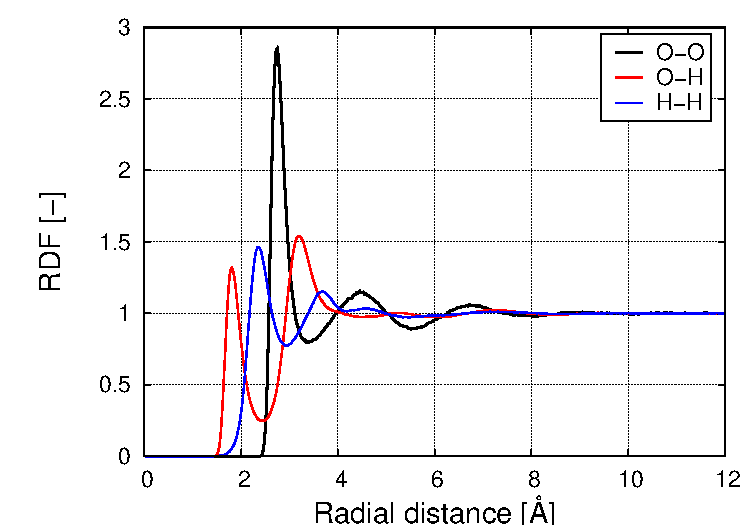
\includegraphics[width=7.5cm]{./Examples/RDFWater.pdf}
  \caption{The radial distribution function of water at 298K.}
  \label{Fig: RDF water}
\end{figure}

\subsection*{Example 9: Computing the radial distribution function of a methane/ethane-mixture}

The radial distribution function (RDF) is a good indication of the status of the fluid: solid, liquid or gas. RASPA
computes the RDF for all (pseudo-)atoms pairs, unless you specified `no' to the `PrintToPDB'-field of the `pseudo\_atoms' file.
For example, the $L$-atoms of water should not be printed to movie-files, and there would be little point generating
the RDF for interactions with these `dummy' interaction sites.
\begin{tiny}
\begin{verbatim}
     SimulationType                MolecularDynamics
     NumberOfCycles                1000000
     NumberOfInitializationCycles  10000
     NumberOfEquilibrationCycles   5000
     PrintEvery                    5000
     
     ContinueAfterCrash            no
     WriteBinaryRestartFileEvery   5000
     
     Ensemble                      NVT
     
     Forcefield                    GarciaPerez2006
     
     Box 0
     BoxLengths 24.0 24.0 24.0
     ComputeRDF yes
     WriteRDFEvery 10000
     RDFHistogramSize 300
     RDFRange 12.0
     ExternalTemperature 300.0
     
     Component 0 MoleculeName             methane
                 MoleculeDefinition       TraPPE
                 TranslationProbability   0.5
                 RotationProbability      0.5
                 ReinsertionProbability   1.0
                 CreateNumberOfMolecules  50
     
     Component 1 MoleculeName             ethane
                 MoleculeDefinition       TraPPE
                 TranslationProbability   0.5
                 RotationProbability      0.5
                 ReinsertionProbability   1.0
                 CreateNumberOfMolecules  50
\end{verbatim}
\end{tiny}

We used the NVT ensemble and therefore we have good temperature control
\begin{tiny}
\begin{verbatim}
     Temperature:             289.880 (avg.  299.641), Translational (avg.  299.641), Rotational (avg.      nan)
     Temperature Adsorbates:  289.880 (avg.  299.641), Translational (avg.  299.641), Rotational (avg.      nan)
\end{verbatim}
\end{tiny}

Shifted potentials are used and the relative energy conservation is 0.0000918675 (excellent).

\subsection*{Example 10: measuring bond/bend/dihedral angle distributions MD}

\begin{tiny}
\begin{verbatim}
     SimulationType                   MolecularDynamics
     NumberOfCycles                   10000000000
     NumberOfInitializationCycles     5000
     NumberOfEquilibrationCycles      10000
     PrintEvery                       10000
     RestartFile                      no
     
     Ensemble NVT
     
     ContinueAfterCrash               no
     WriteBinaryRestartFileEvery      5000
     
     Forcefield                       GarciaPerez2006
     
     Box 0
     BoxLengths 25 25 25
     ExternalTemperature 298.0
     ExternalPressure 0.0
     ComputeMoleculeProperties yes
     
     component 0 MoleculeName                     2-methylbutane
                 StartingBead                     0
                 FugacityCoefficient              1.0
                 MoleculeDefinition               TraPPE
                 TranslationProbability           1.0
                 RotationProbability              1.0
                 RegrowProbability                1.0
                 CBMCProbability                  1.0
                 CreateNumberOfMolecules          32
\end{verbatim}
\end{tiny}

\subsection*{Example 11: measuring bond/bend/dihedral angle distributions MC}


\begin{tiny}
\begin{verbatim}
     SimulationType                   MonteCarlo
     NumberOfCycles                   5000000
     NumberOfInitializationCycles     10000
     PrintEvery                       50000
     RestartFile                      no
     
     ContinueAfterCrash               no
     WriteBinaryRestartFileEvery      50000
     
     Forcefield                       GarciaPerez2006
     
     Box 0
     BoxLengths 25 25 25
     ExternalTemperature 298.0
     ExternalPressure 0.0
     ComputeMoleculeProperties yes
     
     component 0 MoleculeName                     2-methylbutane
                 StartingBead                     0
                 FugacityCoefficient              1.0
                 MoleculeDefinition               TraPPE
                 TranslationProbability           1.0
                 RotationProbability              1.0
                 RegrowProbability                1.0
                 CBMCProbability                  1.0
                 CreateNumberOfMolecules          32
\end{verbatim}
\end{tiny}

\begin{tiny}
\begin{verbatim}
\end{verbatim}
\end{tiny}

\begin{figure}[t]
  \centering
  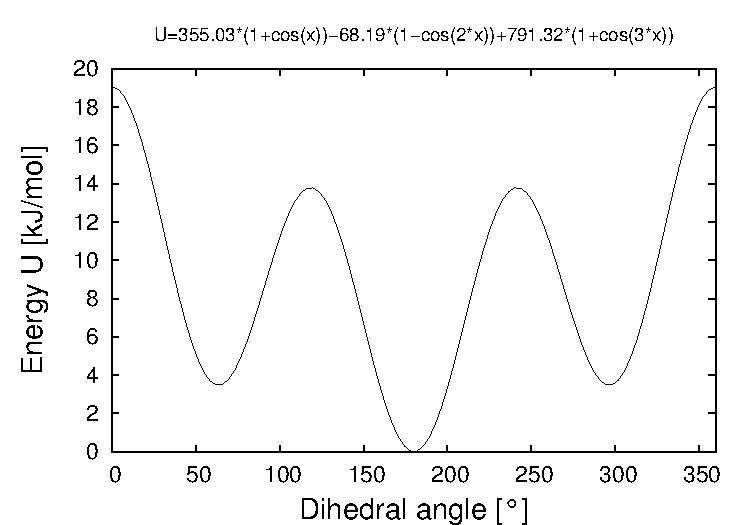
\includegraphics[width=7.5cm]{./Examples/ButaneUADihedral.pdf}
  \caption{The torsion potential for united atom linear alkanes X-CH$_2$-CH$_2$-X.}
  \label{Fig: Butane dihedral}
\end{figure}


\section{Non-basic examples}
\subsection*{Example 1: Adsorption of a binary CO$_2$/CH$_4$ (1:3) mixture in IRMOF-1}

Appreciable adsorption in MOF materials occurs at higher pressure than zeolites, usually in the range up to 10 bar. At these high pressures
absolute and excess adsorption are different, and excess adsorption eventually even goes down. This is due to the fact that excess adsorption is relative
to what would have been in the free pore volume at these conditions. So one can compress the outside fluid but eventually the pores are filled up. At that
maximum absolute loading the excess adsorption will go down.
\begin{tiny}
\begin{verbatim}
     SimulationType                MonteCarlo
     NumberOfCycles                50000
     NumberOfInitializationCycles  5000
     PrintEvery                    1000
     
     Forcefield                    Dubbeldam2007FlexibleIRMOF-1
     
     Framework 0
     FrameworkName IRMOF-1
     UnitCells 1 1 1
     HeliumVoidFraction 0.81
     ExternalTemperature 300.0
     ExternalPressure  10e5
     
     Component 0 MoleculeName               CO2
                 MoleculeDefinition         TraPPE
                 MolFraction                0.25
                 TranslationProbability     0.5
                 RegrowProbability          0.5
                 IdentityChangeProbability  1.0
                   NumberOfIdentityChanges  2
                   IdentityChangesList      0 1
                 SwapProbability            1.0
                 CreateNumberOfMolecules    0
     
     Component 1 MoleculeName               methane
                 MoleculeDefinition         TraPPE
                 MolFraction                0.75
                 TranslationProbability     0.5
                 RegrowProbability          0.5
                 IdentityChangeProbability  1.0
                   NumberOfIdentityChanges  2
                   IdentityChangesList      0 1
                 SwapProbability            1.0
                 CreateNumberOfMolecules    0
\end{verbatim}
\end{tiny}

To compute the excess adsorption the void fraction of a structure needs to be specified using `HeliumVoidFraction [real]'. RASPA automatically uses an
equation of state (default: Peng-Robinson) to compute the fugacities from the pressure and mol-fraction as is done here for a mixture of CO$_2$ and CH$_4$.
It also computes the amount of excess molecules from this equation of state.
\begin{tiny}
\begin{verbatim}
     Component 0 [CO2] (Adsorbate molecule)
     
             Critical temparure [K]: 304.128200
             Critical pressure [Pa]: 7377300.000000
             Acentric factor [-]: 0.223940
     
             RXMC partition factor [-]: 0.000000
     
             Fluid is a vapour
     
             MolFraction:           0.2500000000 [-]
             Compressibility:       0.9714389725 [-]
     
             Density of the bulk fluid phase:      18.1580726483 [kg/m^3]
     
             Binary mixture EOS parameters:  (0): 0.000000 (1): 0.000000
     
             Amount of excess molecules:       0.8675190741 [-]
     
             Conversion factor molecules/unit cell -> mol/kg:       0.1623747175 [-]
             Conversion factor molecules/unit cell -> gr/gr:       7.1442927209 [-]
             Conversion factor molecules/unit cell -> cm^3 STP/gr:       3.6394629804 [-]
             Conversion factor molecules/unit cell -> cm^3 STP/cm^3:       2.1592046669 [-]
             Conversion factor mol/kg -> cm^3 STP/gr:      22.4139757476 [-]
             Conversion factor mol/kg -> cm^3 STP/cm^3:      13.2976654244 [-]
     
             Partial pressure:    250000.00000000000000 [Pa]
                                    1875.00000000000000 [Torr]
                                       2.50000000000000 [bar]
                                       2.46730816679003 [atm]
     
             Fugacity coefficient:       0.9503504709 [-]
     
             Partial fugacity:    237587.61773457148229 [Pa]
                                    1781.90713300928610 [Torr]
                                       2.37587617734571 [bar]
                                       2.34480747825879 [atm]
     
     Component 1 [methane] (Adsorbate molecule)
     
             Critical temparure [K]: 190.564000
             Critical pressure [Pa]: 4599200.000000
             Acentric factor [-]: 0.011420
     
             RXMC partition factor [-]: 0.000000
     
             Fluid is a vapour
     
             MolFraction:           0.7500000000 [-]
             Compressibility:       0.9714389725 [-]
     
             Density of the bulk fluid phase:       6.6206386115 [kg/m^3]
     
             Binary mixture EOS parameters:  (0): 0.000000 (1): 0.000000
     
             Amount of excess molecules:       2.6025572224 [-]
     
             Conversion factor molecules/unit cell -> mol/kg:       0.1623747175 [-]
             Conversion factor molecules/unit cell -> gr/gr:       2.6048899107 [-]
             Conversion factor molecules/unit cell -> cm^3 STP/gr:       3.6394629804 [-]
             Conversion factor molecules/unit cell -> cm^3 STP/cm^3:       2.1592046669 [-]
             Conversion factor mol/kg -> cm^3 STP/gr:      22.4139757476 [-]
             Conversion factor mol/kg -> cm^3 STP/cm^3:      13.2976654244 [-]
     
             Partial pressure:    750000.00000000011642 [Pa]
                                    5625.00000000000091 [Torr]
                                       7.50000000000000 [bar]
                                       7.40192450037010 [atm]
     
             Fugacity coefficient:       0.9790119494 [-]
     
             Partial fugacity:    734258.96201743301935 [Pa]
                                    5506.94221513074717 [Torr]
                                       7.34258962017433 [bar]
                                       7.24657253409754 [atm]
\end{verbatim}
\end{tiny}
Also noteworthy is the use of the identity-change move for mixtures. A molecule of a certain type can be changed at the same position into a molecule of
another type. It is specified per component as a list of other components that are allowed for this move. The identity-change move is highly recommended
at high loadings.

At each `PrintEvery' steps the loadings are shown in a variety of units for both excess and absolute adsorption:
\begin{tiny}
\begin{verbatim}
     Loadings per component:
     ----------------------------------------------------------------------------------------------------------------------------------------------------------------------
     Component 0 (CO2), current number of integer/fractional/reaction molecules: 16/0/0 (avg.  12.68484), density:  67.81662 (avg.  53.76520) [kg/m^3]
             absolute adsorption:  16.00000 (avg.  12.68484) [mol/uc],   2.5979954802 (avg.   2.0596978259) [mol/kg], 114.3086835349 (avg.  90.6242327003) [mg/g]
                                   58.2314076859 (avg.  46.1660171161) [cm^3 STP/g],   34.5472746700 (avg.  27.3891725636) [cm^3 STP/cm^3]
             excess adsorption:    15.1324809259 (avg.  11.8173240923) [mol/uc],   2.4571323156 (avg.   1.9188346613) [mol/kg], 108.1108733282 (avg.  84.4264224936) [mg/g]
                                   55.0741041308 (avg.  43.0087135610) [cm^3 STP/g],   32.6741234365 (avg.  25.5160213301) [cm^3 STP/cm^3]
     Component 1 (methane), current number of integer/fractional/reaction molecules: 19/0/0 (avg.  19.21646), density:  29.36296 (avg.  29.69749) [kg/m^3]
             absolute adsorption:  19.00000 (avg.  19.21646) [mol/uc],   3.0851196328 (avg.   3.1202680711) [mol/kg],  49.4929083037 (avg.  50.0567757203) [mg/g]
                                   69.1497966270 (avg.  69.9376128722) [cm^3 STP/g],   41.0248886706 (avg.  41.4922808443) [cm^3 STP/cm^3]
             excess adsorption:    16.3974427776 (avg.  16.6139077477) [mol/uc],   2.6625301390 (avg.   2.6976785773) [mol/kg],  42.7135332529 (avg.  43.2774006695) [mg/g]
                                   59.6778859617 (avg.  60.4657022069) [cm^3 STP/g],   35.4054349701 (avg.  35.8728271438) [cm^3 STP/cm^3]
     ----------------------------------------------------------------------------------------------------------------------------------------------------------------------
\end{verbatim}
\end{tiny}
and at the end error bars are computed for all properties:
\begin{tiny}
\begin{verbatim}
     Component 0 [CO2]
     -------------------------------------------------------------
             Block[ 0] 12.55000           [-]
             Block[ 1] 12.79110           [-]
             Block[ 2] 12.75510           [-]
             Block[ 3] 12.73990           [-]
             Block[ 4] 12.58240           [-]
             ------------------------------------------------------------------------------
             Average                                     12.6837000000 +/-       0.1958132580 [-]
             Average loading absolute [molecules/unit cell]       12.6837000000 +/-       0.1958132580 [-]
             Average loading absolute [mol/kg framework]          2.0595122045 +/-       0.0317951224 [-]
             Average loading absolute [milligram/gram framework]         90.6160655845 +/-       1.3989472336 [-]
             Average loading absolute [cm^3 (STP)/gr framework]         46.1618566041 +/-       0.7126551035 [-]
             Average loading absolute [cm^3 (STP)/cm^3 framework]         27.3867042332 +/-       0.4228009005 [-]
     
             Average loading excess [molecules/unit cell]       11.8161809259 +/-       0.1958132580 [-]
             Average loading excess [mol/kg framework]          1.9186490399 +/-       0.0317951224 [-]
             Average loading excess [milligram/gram framework]         84.4182553778 +/-       1.3989472336 [-]
             Average loading excess [cm^3 (STP)/gr framework]         43.0045530490 +/-       0.7126551035 [-]
             Average loading excess [cm^3 (STP)/cm^3 framework]         25.5135529997 +/-       0.4228009005 [-]
     
     Component 1 [methane]
     -------------------------------------------------------------
             Block[ 0] 19.23430           [-]
             Block[ 1] 19.30250           [-]
             Block[ 2] 19.22250           [-]
             Block[ 3] 19.11980           [-]
             Block[ 4] 19.19560           [-]
             ------------------------------------------------------------------------------
             Average                                     19.2149400000 +/-       0.1184039594 [-]
             Average loading absolute [molecules/unit cell]       19.2149400000 +/-       0.1184039594 [-]
             Average loading absolute [mol/kg framework]          3.1200204545 +/-       0.0192258095 [-]
             Average loading absolute [milligram/gram framework]         50.0528033411 +/-       0.3084292792 [-]
             Average loading absolute [cm^3 (STP)/gr framework]         69.9320628000 +/-       0.4309268269 [-]
             Average loading absolute [cm^3 (STP)/cm^3 framework]         41.4889881217 +/-       0.2556583817 [-]
     
             Average loading excess [molecules/unit cell]       16.6123827776 +/-       0.1184039594 [-]
             Average loading excess [mol/kg framework]          2.6974309607 +/-       0.0192258095 [-]
             Average loading excess [milligram/gram framework]         43.2734282903 +/-       0.3084292792 [-]
             Average loading excess [cm^3 (STP)/gr framework]         60.4601521347 +/-       0.4309268269 [-]
             Average loading excess [cm^3 (STP)/cm^3 framework]         35.8695344212 +/-       0.2556583817 [-]
\end{verbatim}
\end{tiny}


\subsection*{Example 2: NPT Monte Carlo of propane}

The density of propane at 250K and 10 bar is about 559.53 kg/m$^3$ (NIST database). In this example the density is
computed using Monte Carlo in the NPT-ensemble. Given the pressure $P$, the temperature $T$, and the amount of molecules $N$,
the density is computed.

\begin{tiny}
\begin{verbatim}
     SimulationType                MonteCarlo
     NumberOfCycles                50000
     NumberOfInitializationCycles  10000
     PrintEvery                    1000
     RestartFile                   no
     
     Forcefield                    GarciaPerez2006
     
     Box 0
     BoxLengths 30 30 30
     ExternalTemperature 250.0
     ExternalPressure 1e6
     ComputeMolecularPressure yes
     
     VolumeChangeProbability       0.05
     
     Component 0 MoleculeName             propane
                 MoleculeDefinition       TraPPE
                 TranslationProbability   0.5
                 RotationProbability      0.5
                 RegrowProbability        0.5
                 CreateNumberOfMolecules  256
\end{verbatim}
\end{tiny}

The TraPPE model for propane gives for our simulation of 25000 cycles $568.2\pm 4.1$ kg/m$^3$.
The measured pressure is $9.75\pm2.2$ bar.


\subsection*{Example 3: NPT molecular dynamics of water}
A molecular dynamics simulation of water in the NPT-ensemble
(constant amount of particles $N$, constant average pressure $P$, and constant average temperature $T$).
Many water models are defined, but most are defined with simple Coulombic potentials using cutoffs of 9\AA.
None are optimized with the Ewald-summation except for the recalibrated Tip5p-Ew model.
Unfortunately, that model is defined using a cutoff always equal to half the box size, while
RASPA uses a fixed cutoff (default: 12 Angstrom). A fixed cutoff is more realistic, but requires the shortest
perpendicular width to be twice the cutoff, thus here larger than 24 \AA. All this results in having
to simulate more than 512 water molecules. The tip5p models use 5 fixed charges placed in the water geometry,
so for each step 2560 charge sites needs to be computed with Ewald. Conclusion: liquid water is computationally
expensive to compute when done properly.

In MD-NPT the average pressure 
$\left\langle P\right\rangle$ and average temperature $\left\langle T\right\rangle$ are imposed. The instantaneous
values, especially for the pressure, are different. RASPA uses the Nose-Hoover chain method, and NPT-MD methods of
Martyna and Tuckermann.

Several options are introduced here: "TimeStep [real]" to set the time step. For rigid molecules the time step can be a bit larger
because the high frequency movement is removed (the O-H is around 3000 cm$^{-1}$). The cutoff can be set with `CutOff [real]'.
The method to compute charge interactions is set with `ChargeMethod [Ewald$|$None]', although Ewald is the default. The precision can specified
using `EwaldPrecision [real]' from which the Ewald parameters $\kappa$ and the amount of wave vectors is inferred.
The initial positions of the water are read from file (`RestartFile yes'), the file is located in directory `RestartInitial/System[int]'.

The experimental density of water at 300K and 1 bar is about 996.56 kg/m$^3$ (NIST database).

\begin{tiny}
\begin{verbatim}
     SimulationType                MolecularDynamics
     NumberOfCycles                100000
     NumberOfInitializationCycles  0
     NumberOfEquilibrationCycles   1000
     PrintEvery                    100
     RestartFile                   yes

     Ensemble                      NPT
     TimeStep                      0.001

     ChargeMethod                  Ewald
     CutOff                        10.0
     Forcefield                    Tip5p-Ew
     EwaldPrecision                1e-6

     Box 0
     BoxLengths 24.83 24.83 24.83
     ExternalTemperature 300.0
     ExternalPressure 1.0e5
     ComputeMSD yes
     PrintMSDEvery 5000

     Component 0 MoleculeName             Tip5p
                 StartingBead             0
                 MoleculeDefinition       Water
                 TranslationProbability   1.0
                 RotationProbability      1.0
                 ReinsertionProbability   1.0
                 CreateNumberOfMolecules  0
\end{verbatim}
\end{tiny}

The output shows some details of intermediate status during the run: the time run, the current box and average box, etc.
The total linear momentum is conserved and zero (the center of mass movement of the system is removed at initialization).
For this relatively short run, the average pressure of 1.26 bar is already quite close to the applied 1 bar.
Also, the temperature of the water, and of the simulation cell (it is a degree of freedom and has therefore an associated temperature)
can also been seen to converge to the applied value of 300K. Energy conservation is adequate with a 0.001 ps time step.
\begin{tiny}
\begin{verbatim}
TODO
\end{verbatim}
\end{tiny}


\subsection*{Example 4: Adsorption of CO$_2$ in Na-LTA}

The Linde Type A structure LTA-4A has 96 aluminum per unit cell. A common 4A sample has 96 charge balancing sodium ions.
The ions are small enough to access the sodalite cages, but the bigger methane molecules are exclusively in the big $\alpha$-cages
and not in the sodalite cages. They need to be artificially blocked. 
Because the adsorption is dependent on the positions of the ions it is
important to start from the crystallographic positions and use \emph{only} translation for the ions. Reinsertion moves may transport the ions
to positions in the windows and this is especially important for diffusion (the next example).

\begin{tiny}
\begin{verbatim}
     SimulationType                   MonteCarlo
     NumberOfCycles                   25000
     NumberOfInitializationCycles     10000
     RestartFile                      no
     PrintEvery                       1000
     
     Forcefield                       GarciaPerez2006
     ModifyOxgensConnectedToAluminium yes
     
     Framework 0
     FrameworkName LTA4A
     RemoveAtomNumberCodeFromLabel yes
     UnitCells 1 1 1
     ExternalTemperature 298.0
     ExternalPressure 10000.0
     
     Component 0 MoleculeName                   sodium
                 MoleculeDefinition             TraPPE
                 TranslationProbability         1.0
                 RandomTranslationProbability   1.0
                 ExtraFrameworkMolecule         yes
                 CreateNumberOfMolecules        96
     
     Component 1 MoleculeName                   CO2
                 MoleculeDefinition             TraPPE
                 BlockPockets                   yes
                 BlockPocketsFilename           LTA
                 TranslationProbability         1.0
                 ReinsertionProbability         1.0
                 SwapProbability                1.0
                 ExtraFrameworkMolecule         no
                 CreateNumberOfMolecules        0
\end{verbatim}
\end{tiny}

\subsection*{Example 5: Diffusion of CO$_2$ in Na-LTA}

An example of molecular dynamics of an adsorbate (CO$_2$) diffusing through the pores of LTA 4A loaded with ions.
The ions are read from the restart-file. The mean-square displacement is computed during the run.

\begin{tiny}
\begin{verbatim}
     SimulationType                   MolecularDynamics
     NumberOfCycles                   250000
     NumberOfInitializationCycles     5000
     NumberOfEquilibrationCycles      10000
     PrintEvery                       5000
     RestartFile                      no
     
     Ensemble                         NVT
     
     Forcefield                       GarciaPerez2006
     ModifyOxgensConnectedToAluminium yes
     TimeStep                         0.0005
     
     Framework 0
     FrameworkName LTA4A
     RemoveAtomNumberCodeFromLabel yes
     UnitCells 1 1 1
     ExternalTemperature 600.0
     ComputeMSD yes
     PrintMSDEvery 5000
     
     component 0 MoleculeName             sodium
                 MoleculeDefinition       TraPPE
                 TranslationProbability   1.0
                 ReinsertionProbability   1.0
                 ExtraFrameworkMolecule   yes
                 CreateNumberOfMolecules  96
     
     component 1 MoleculeName             CO2
                 MoleculeDefinition       TraPPE
                 BlockPockets             yes
                 BlockPocketsFilename     LTA
                 TranslationProbability   1.0
                 RotationProbability      1.0
                 ReinsertionProbability   1.0
                 ExtraFrameworkMolecule   no
                 CreateNumberOfMolecules  64
\end{verbatim}
\end{tiny}

\subsection*{Example 6: Diffusion of benzene in rigid IRMOF-1}

Benzene (and aromatic molecules in general) are usually kept rigid. RASPA uses quaternions for the description of the
orientation of the molecules. The integration schemes of Martyna and Tuckermann are symplectic and conserve energy
very well. Even though the molecule is described as a center of mass and a orientation, the forces are still computed
atomically. In this example the diffusivity the mean-square displacement of benzene at 298K in IRMOF-1 is computed.
The forcefield is `FlexibleIRMOF-1' which is also perfectly suitable for rigid structures. It has been specifically
optimized for iso-reticular metal-organic frameworks.

\begin{tiny}
\begin{verbatim}
     SimulationType                MolecularDynamics
     NumberOfCycles                100000
     NumberOfEquilibrationCycles   10000
     NumberOfInitializationCycles  1000
     PrintEvery                    5000
     RestartFile                   no
     
     Ensemble                      NVT
     
     ChargeMethod                  Ewald
     CutOff                        12.0
     TimeStep                      0.0005
     Forcefield                    Dubbeldam2007FlexibleIRMOF-1
     EwaldPrecision                1e-6
     
     Framework 0
     FrameworkName IRMOF-1
     UnitCells 1 1 1
     ExternalTemperature 298.0
     
     Component 0 MoleculeName              benzene
                 StartingBead              0
                 MoleculeDefinition        TraPPE
                 IdealGasRosenbluthWeight  1.0
                 TranslationProbability    1.0
                 RotationProbability       1.0
                 RegrowProbability         1.0
                 CreateNumberOfMolecules   16
\end{verbatim}
\end{tiny}

\begin{figure}[t]
  \centering
  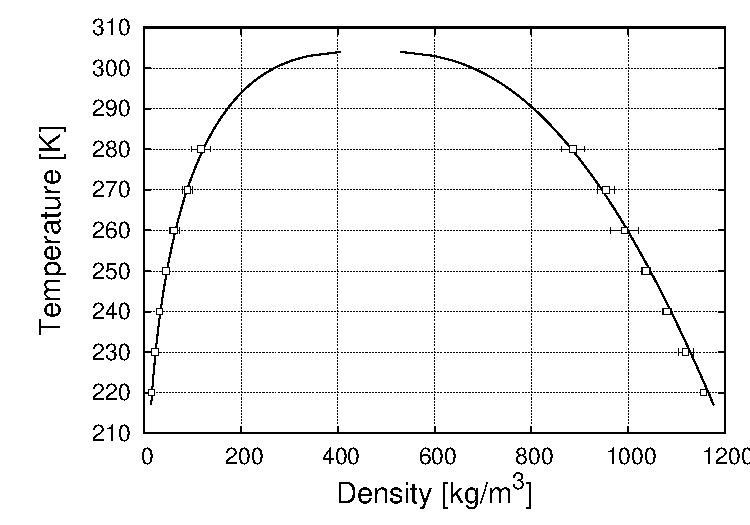
\includegraphics[width=7.5cm]{./Examples/GibbsCO2.pdf}
  \caption{Gibbs ensemble simulation of CO2 at 250K. Two simulation boxes are used: one for the gas-branch and one for the liquid branch. The simulation can
           only be conducted below a certain temperature because otherwise the boxes can swap between gas and liquid. At 250K, the boxes are initialized
           with an equal amount of molecules, but soon split into gas and liquid. The average densities are straightforward to measure. As shown, the
           TraPPE model for CO2 does a good job when compare to experimental data (NIST database).}
  \label{Fig: Gibbs CO2}
\end{figure}

\subsection*{Example 7: Gibbs ensemble simulation of CO$_2$}

The Gibbs ensemble is way of computing coexistence without interfaces. It is one the most used methods
to study vapor-liquid and liquid-liquid equilibria, it is not suitable for very dense systems. The 
conditions for coexistence of two or more phases I, II, \dots is that the pressure and temperature 
of all the phases must be equal, as well as the chemical potential of all the species. The Gibbs
ensemble example for the single component CO$_2$ is listed below. two boxes will be used, one will
correspond to the liquid phase, the other one to the gas phase. The `GibbsVolumeChange' move
changes the individual volume leaving the total volume in tact, the `GibbsSwap' move
swaps particles from one box to the other. One of the practical problems is to make sure both
boxes remain larger than twice the cutoff length. If not, the program will exit with an error message,
and the simulation should be restarted with a bigger volume. 
Note that RASPA uses orientational biased insertions for small rigid molecules like CO$_2$.
For this example about 10000-20000 cycles are needed to equilibrate properly.
\begin{tiny}
\begin{verbatim}
     SimulationType                MonteCarlo
     NumberOfCycles                25000
     NumberOfInitializationCycles  10000
     PrintEvery                    1000
     RestartFile                   no
     
     Forcefield                    TraPPE
     
     Box 0
     BoxLengths 30 30 30
     BoxAngles 90 90 90
     ExternalTemperature 240.0
     
     Box 1
     BoxLengths 30 30 30
     BoxAngles 90 90 90
     ExternalTemperature 240.0
     
     GibbsVolumeChangeProbability 0.1
     
     Component 0 MoleculeName             CO2
                 StartingBead             1
                 MoleculeDefinition       TraPPE
                 TranslationProbability   1.0
                 RotationProbability      1.0
                 ReinsertionProbability   1.0
                 GibbsSwapProbability     1.0
                 CreateNumberOfMolecules  150 150
\end{verbatim}
\end{tiny}

\subsection*{Example 8: Minimization of a flexible framework (fixed volume)}

Physically, energy minimization corresponds to an instantaneous freezing of the system; a static structure in 
which no atom feels a net force corresponds to a temperature of 0 K. In the early 1980's, energy minimization was 
about all one could afford to do and was dubbed `molecular mechanics.' Here, a difficult optimization problem:
a flexible framework, IRMOF-1, in a periodic unit cell, with many low energy modes.
The energy landscape of a framework is very complex. A true minimum is characterized by
all positive eigenvalues of the Hessian matrix (the matrix of second derivatives with respect to position). A
zero eigenvalue means that moving in the direction of the associated eigenvector does not result in a change in
energy. Likewise, a negative en positive eigenvalue means an decrease and increase in energy, respectively.
Most of the optimization time is spent on reaching a zero curvature structure, i.e. all positive eigenvalues.

\begin{tiny}
\begin{verbatim}
     SimulationType  Minimization
     NumberOfCycles  1
     RestartFile     no
     PrintEvery      1
     
     MaximumNumberOfMinimizationSteps 1000
     RMSGradientTolerance 1e-6
     MaxGradientTolerance 1e-6
     
     Ensemble        NVT
     
     Forcefield                                 Dubbeldam2007FlexibleIRMOF-1
     ChargeMethod                               Ewald
     EwaldPrecision                             1e-10
     InternalFrameworkLennardJonesInteractions  yes
     
     Framework 0
     FrameworkName IRMOF-1
     UnitCells 1 1 1
     ExternalTemperature 298.0
     Movies yes
     WriteMoviesEvery 1
     
     FlexibleFramework     yes
     FrameworkDefinitions  Dubbeldam2007FlexibleIRMOF-1
\end{verbatim}
\end{tiny}
The minimization needs 119 cycles to optimize IRMOF-1, the last steps are shown here. The convergence is very rapid (quadratic) near the minimum,
and the minimum energy can be reached up to arbitrary precision (the forces on all the atoms are $1\times10^{-8}$ K/\AA$^2$
or smaller). To compute spectra, frequencies and/or eigenmodes a high precision is needed.
\begin{tiny}
\begin{verbatim}
     Starting configuration:
           Box:      25.8320000000       0.0000000000       0.0000000000     Strain derivative:  129316.6369463501       0.0000000016       0.0000000015
                      0.0000000000      25.8320000000       0.0000000000                              0.0000000015  129316.6369463478       0.0000000016
                      0.0000000000       0.0000000000      25.8320000000                              0.0000000016       0.0000000015  129316.6369463608


     Beginning Baker minimization:
     -----------------------------
     Shifting parameter: -144554.0050033366 Lowest eigenvalue:   -1933.2972944159
     Iteration: 0 Energy: -4210346.0956447003 RMS gradient: 254.796  Max gradient: 16621.7 Number of negative eigenvalues: 30 Number of zero eigenvalues: 3
           Box:      25.8320000000       0.0000000000       0.0000000000     Strain derivative:  129316.6369463581       0.0000000016       0.0000000015
                      0.0000000000      25.8320000000       0.0000000000                              0.0000000016  129316.6369463568       0.0000000016
                      0.0000000000       0.0000000000      25.8320000000                              0.0000000015       0.0000000016  129316.6369463690
           Lengths:      25.8320000000      25.8320000000      25.8320000000, Angles:      90.0000000000      90.0000000000      90.0000000000

     Shifting parameter:  -54112.0433245863 Lowest eigenvalue:    -942.0341042027
     Iteration: 1 Energy: -4291359.2884553447 RMS gradient: 132.811  Max gradient: 9119.05 Number of negative eigenvalues: 30 Number of zero eigenvalues: 3
           Box:      25.8320000000       0.0000000000       0.0000000000     Strain derivative: -131739.2152028512       0.0000000004       0.0000000008
                      0.0000000000      25.8320000000       0.0000000000                              0.0000000004 -131739.2152028439       0.0000000010
                      0.0000000000       0.0000000000      25.8320000000                              0.0000000008       0.0000000011 -131739.2152028617
           Lengths:      25.8320000000      25.8320000000      25.8320000000, Angles:      90.0000000000      90.0000000000      90.0000000000

     Shifting parameter:   -6990.6349276451 Lowest eigenvalue:    -218.9092550725
     Iteration: 2 Energy: -4325503.0430874182 RMS gradient: 38.7491  Max gradient: 2721.14 Number of negative eigenvalues: 36 Number of zero eigenvalues: 3
           Box:      25.8320000000       0.0000000000       0.0000000000     Strain derivative: -282155.2863533634       0.0000000002       0.0000000007
                      0.0000000000      25.8320000000       0.0000000000                              0.0000000002 -282155.2863533496      -0.0000000021
                      0.0000000000       0.0000000000      25.8320000000                              0.0000000008      -0.0000000021 -282155.2863533603
           Lengths:      25.8320000000      25.8320000000      25.8320000000, Angles:      90.0000000000      90.0000000000      90.0000000000

     ..........................................................................

     Iteration: 117 Energy: -4331364.7259515934 RMS gradient: 0.00439145  Max gradient: 0.600384 Number of negative eigenvalues: 0 Number of zero eigenvalues: 3
           Box:      25.8320000000       0.0000000000       0.0000000000     Strain derivative:  -99169.3483007069       0.0011594244       0.0002624505
                      0.0000000000      25.8320000000       0.0000000000                              0.0011594245  -99108.1188463482      -0.0004447560
                      0.0000000000       0.0000000000      25.8320000000                              0.0002624506      -0.0004447560  -99128.0909746577
           Lengths:      25.8320000000      25.8320000000      25.8320000000, Angles:      90.0000000000      90.0000000000      90.0000000000

     Iteration: 118 Energy: -4331364.6575047411 RMS gradient: 7.06135e-05  Max gradient: 0.0204619 Number of negative eigenvalues: 0 Number of zero eigenvalues: 3
           Box:      25.8320000000       0.0000000000       0.0000000000     Strain derivative:  -99208.8822655176       0.0000019593      -0.0000031410
                      0.0000000000      25.8320000000       0.0000000000                              0.0000019594  -99184.4522480669      -0.0000004895
                      0.0000000000       0.0000000000      25.8320000000                             -0.0000031410      -0.0000004895  -99202.7818375186
           Lengths:      25.8320000000      25.8320000000      25.8320000000, Angles:      90.0000000000      90.0000000000      90.0000000000

     Iteration: 119 Energy: -4331364.6575191850 RMS gradient: 6.91407e-07  Max gradient: 8.83309e-05 Number of negative eigenvalues: 0 Number of zero eigenvalues: 3
           Box:      25.8320000000       0.0000000000       0.0000000000     Strain derivative:  -99195.5973070737       0.0000000048      -0.0000030267
                      0.0000000000      25.8320000000       0.0000000000                              0.0000000047  -99195.5991107764       0.0000000006
                      0.0000000000       0.0000000000      25.8320000000                             -0.0000030267       0.0000000006  -99195.6111130547
           Lengths:      25.8320000000      25.8320000000      25.8320000000, Angles:      90.0000000000      90.0000000000      90.0000000000

     SUCCES: RMS Gradient tolerance 0.0001 reached (6.91407e-07)
             Max Gradient tolerance 0.0001 reached (8.83309e-05)


\end{verbatim}
\end{tiny}
The shifting values are always lower than the lowest eigenvalues, both are negative and approach zero. At iteration 2, the lowest eigenvalues is closer
to zero, but still the amount of negative eigenvalues is 6 higher. Also increases in energy can occur. However, eventually the system is driven to
all positive eigenvalues (a true energy minimum without saddle points) and the lowest energy.
Note that minimization the structure in constant volume results in a finite (non-zero) stress. Minimization taking volume and shape changes into account
are usually easier, because the system is less constrained.
If one would like to also minimize the cell volume (isotropicly) use
\begin{tiny}
\begin{verbatim}
     Ensemble                         NPT
\end{verbatim}
\end{tiny}
or use for a change in cell-lengths and cell-angles
\begin{tiny}
\begin{verbatim}
     Ensemble                         NPTPR
\end{verbatim}
\end{tiny}


\section{Advanced examples}

\subsection*{Example 1: Adsorption of CO$_2$ in fully-flexible IRMOF-1 ($\mu VT$-ensemble)}

Flexibility in MOFs is more important than in zeolites. A very efficient move to change the whole framework (and actually
also the adsorbates) is have a short NVE MD-run and accept or reject the new configuration. This hybrid MD/MC move can be switched on using
`HybridMCMDMoveProbability  [real]', where [real] is the fraction of the move at each cycle.

\begin{tiny}
\begin{verbatim}
     SimulationType                MonteCarlo
     NumberOfCycles                50000
     NumberOfInitializationCycles  20000
     PrintEvery                    5000
     RestartFile                   no
     
     ChargeMethod                  Ewald
     CutOff                        12.0
     Forcefield                    Dubbeldam2007FlexibleIRMOF-1
     EwaldPrecision                1e-6
     
     Framework 0
     FrameworkName IRMOF-1
     UnitCells 1 1 1
     HeliumVoidFraction 0.801937
     FrameworkDefinitions Dubbeldam2007FlexibleIRMOF-1
     ExternalTemperature 233.0
     ExternalPressure  1e5
     
     FlexibleFramework yes
     
     HybridMCMDMoveProbability 1.0
     
     Component 0 MoleculeName              CO2
                 StartingBead              0
                 MoleculeDefinition        TraPPE
                 IdealGasRosenbluthWeight  1.0
                 TranslationProbability    1.0
                 RotationProbability       1.0
                 ReinsertionProbability    1.0
                 SwapProbability           1.0
                 CreateNumberOfMolecules   0
\end{verbatim}
\end{tiny}


\subsection*{Example 2: CO$_2$ adsorption in flexible IRMOF-1 (osmotic ensemble).}

Adsorption simulations using a flexible framework are very computationally demanding, the current example will 
probably run about a week. The equilibration is very important and it is best to start with a restart-file
obtained from the previous example at the same temperature. The directory `Restart' produced in the previous
example should be copied to `RestartInitial' and the option `RestartFile' should be set to `yes'.

\begin{tiny}
\begin{verbatim}
     SimulationType                MonteCarlo
     NumberOfCycles                50000
     NumberOfInitializationCycles  10000
     PrintEvery                    5000
     RestartFile                   no
     
     ChargeMethod                  Ewald
     CutOff                        12.0
     Forcefield                    Dubbeldam2007FlexibleIRMOF-1
     EwaldPrecision                1e-6
     TimeStep                      0.0005
     
     Framework 0
     FrameworkName IRMOF-1
     UnitCells 1 1 1
     HeliumVoidFraction 0.801937
     ExternalTemperature 298.0
     ExternalPressure 100e3
     
     FrameworkDefinitions Dubbeldam2007FlexibleIRMOF-1
     FlexibleFramework yes
     
     HybridNVEMoveProbability 1.0
       NumberOfHybridNVESteps 5
     VolumeChangeProbability  1.0
     
     Component 0 MoleculeName              CO2
                 StartingBead              0
                 MoleculeDefinition        TraPPE
                 IdealGasRosenbluthWeight  1.0
                 TranslationProbability    1.0
                 RotationProbability       1.0
                 ReinsertionProbability    1.0
                 SwapProbability           1.0
                 CreateNumberOfMolecules   0
\end{verbatim}
\end{tiny}

\subsection*{Example 3: NPT molecular dynamics of flexible IRMOF-1}

An NPT-ensemble simulation of a flexible framework IRMOF-1. This type of simulation can be used to compute the average
unit cell size at the desired temperature and pressure (and properties like the `volumetric expansion coefficient' etc).
The equilibration, although slow, is very much faster than Monte Carlo. The example show the code for flexible
IRMOF-1 at 298K and 1 atm.

\begin{tiny}
\begin{verbatim}
     SimulationType               MolecularDynamics
     NumberOfCycles               500000
     NumberOfEquilibrationCycles  5000
     PrintEvery                   5000
     RestartFile                  no
     
     Ensemble                     NPT
     
     Forcefield                   Dubbeldam2007FlexibleIRMOF-1
     CutOff                       12.0
     
     Framework 0
     FrameworkName IRMOF-1
     UnitCells 1 1 1
     ExternalTemperature 298.0
     ExternalPressure 101325.0
     
     FlexibleFramework yes
     FrameworkDefinitions Dubbeldam2007FlexibleIRMOF-1
\end{verbatim}
\end{tiny}


\subsection*{Example 4: Benzene diffusion in flexible IRMOF-10}

Molecules with a phenyl-ring are usually quite rigid. In Monte Carlo rigid units are not a problem, because the MC moves can be developed in such a way that the
constraints remain satisfied, i.e. translation and rotation of the whole rigid unit. In molecular dynamics, there are two general approaches. The first is to integrate
the molecules atomically and afterwards satisfy the constraints iteratively using for example the shake algorithm. For bigger molecules complications arise, convergence
becomes more difficult, and for a planar molecule like benzene additional sites above the molecule are needed. Therefore, the second approach has become more popular. 
Using quaternions (or Euler angles) one can describe the configurations of the molecule as a center-of-mass position and an orientation. The translation and rotation
are integrated and when the forces are needed the atoms positions are computed from the com position and the orientation. The forces are then summed to the center of mass
and the torque is computed. Miller et al. have developed an integration algorithm for rigid units (using quaternions) that is symplectic.

All these techniques are combined in the example of diffusion of benzene in IRMOF-10. The integration is performed in the NVT ensemble using the Nose-Hoover thermostats.
Three separate NH chains are operating on (i) the translation, (ii) the rotation of the molecules, and (iii) on the framework.

\begin{tiny}
\begin{verbatim}
     SimulationType                MolecularDynamics
     NumberOfCycles                1000000
     NumberOfEquilibrationCycles   10000
     NumberOfInitializationCycles  100
     PrintEvery                    5000
     RestartFile                   no
     
     Ensemble                      NVT
     
     ChargeMethod                  Ewald
     CutOff                        12.0
     TimeStep                      0.0005
     Forcefield                    Dubbeldam2007FlexibleIRMOF-10
     EwaldPrecision                1e-6
     
     Framework 0
     FrameworkName IRMOF-10
     UnitCells 1 1 1
     ExternalTemperature 298.0
     Movies no
     WriteMoviesEvery 1000
     
     FrameworkDefinitions Dubbeldam2007FlexibleIRMOF-10
     FlexibleFramework yes
     
     Component 0 MoleculeName              benzene
                 StartingBead              0
                 MoleculeDefinition        TraPPE
                 IdealGasRosenbluthWeight  1.0
                 TranslationProbability    1.0
                 RotationProbability       1.0
                 ReinsertionProbability    1.0
                 CreateNumberOfMolecules   16
\end{verbatim}
\end{tiny}

\subsection*{Example 5: Continuous Fractional Component Monte Carlo}

A mixture simulation of CO2 and N2 in DMOF. The charges of DMOF are listed in the CIF-File using the `\_atom\_site\_charge' keyword,
and RASPA makes use of these usinf the keyword `UseChargesFromCIFFile yes'.
The CFCMC method is switched on by using `CFSwapLambdaProbability' (instead of `SwapProbability') to swap molecules in and out of the system at a fixed fugacity.
The biasing factors are measured using Wang-Landau sampling during `NumberOfEquilibrationCycles 50000'.

\begin{tiny}
\begin{verbatim}
     SimulationType                MonteCarlo
     NumberOfCycles                250000
     NumberOfEquilibrationCycles   50000
     PrintEvery                    5000
     RestartFile                   no
     
     ContinueAfterCrash no
     WriteBinaryRestartFileEvery 5000
     
     ChargeMethod                  Ewald
     Forcefield                    local
     CutOffVDW                     11.5
     RemoveAtomNumberCodeFromLabel no
     
     Framework             0
     FrameworkName         DMOF
     UseChargesFromCIFFile yes
     UnitCells             1 1 1
     HeliumVoidFraction    0.614
     ExternalTemperature   300
     ExternalPressure      1e5
     
     Component 0 MoleculeName              CO2
                 StartingBead              0
                 MoleculeDefinition        TraPPE
                 IdealGasRosenbluthWeight  1
                 FugacityCoefficient       1.0
                 TranslationProbability    1.0
                 RotationProbability       1.0
                 ReinsertionProbability    1.0
                 CBMCProbability           0.0
                 IdentityChangeProbability 1.0
                   NumberOfIdentityChanges 2
                   IdentityChangesList     0 1
                 SwapProbability           0.0
                 CFSwapLambdaProbability   1.0
                 CreateNumberOfMolecules   0
     
     Component 1 MoleculeName              N2
                 StartingBead              0
                 MoleculeDefinition        TraPPE
                 IdealGasRosenbluthWeight  1
                 FugacityCoefficient       1.0
                 TranslationProbability    1.0
                 RotationProbability       1.0
                 ReinsertionProbability    1.0
                 CBMCProbability           0.0
                 IdentityChangeProbability 1.0
                   NumberOfIdentityChanges 2
                   IdentityChangesList     0 1
                 SwapProbability           0.0
                 CFSwapLambdaProbability   1.0
                 CreateNumberOfMolecules   0
\end{verbatim}
\end{tiny}

The performance of the CFCMC is written at the end of the output file (after the run has finished).
The biasing factors have lead to relatively flat distribution of Lambda. The efficiency of insertion is
much higher (sometimes dramatically higher) than using conventional MC or even CBMC.

\begin{tiny}
\begin{verbatim}
     Performance of the CFMC swap lambda move:
     =========================================
     Component [CO2] total tried: 609238.000000 constant-lambda accepted: 378163.000000 (62.071473 [%])
                    total tried: 306306.000000 insert-lambda accepted: 75081.000000 (24.511763 [%])
                    total tried: 303052.000000 remove-lambda accepted: 75005.000000 (24.749878 [%])
     
             Lambda probabilities:
             ---------------------
             Lambda [ 0.000000 - 0.047619 ]:       4.6286053786 (biasing factor:       0.0000000000)
             Lambda [ 0.047619 - 0.095238 ]:       4.8557520294 (biasing factor:      -0.0382812500)
             Lambda [ 0.095238 - 0.142857 ]:       4.5367783909 (biasing factor:      -0.1300000000)
             Lambda [ 0.142857 - 0.190476 ]:       4.8916129710 (biasing factor:      -0.1393750000)
             Lambda [ 0.190476 - 0.238095 ]:       5.0546694721 (biasing factor:      -0.1734375000)
             Lambda [ 0.238095 - 0.285714 ]:       4.5641049207 (biasing factor:      -0.3854687500)
             Lambda [ 0.285714 - 0.333333 ]:       4.7402092244 (biasing factor:      -0.4912500000)
             Lambda [ 0.333333 - 0.380952 ]:       4.7959290856 (biasing factor:      -0.6443750000)
             Lambda [ 0.380952 - 0.428571 ]:       4.8145570804 (biasing factor:      -0.8160937500)
             Lambda [ 0.428571 - 0.476190 ]:       4.5662385237 (biasing factor:      -1.0582812500)
             Lambda [ 0.476190 - 0.523810 ]:       4.7369267583 (biasing factor:      -1.2257812500)
             Lambda [ 0.523810 - 0.571429 ]:       4.6820275136 (biasing factor:      -1.4496875000)
             Lambda [ 0.571429 - 0.619048 ]:       4.7426710739 (biasing factor:      -1.6581250000)
             Lambda [ 0.619048 - 0.666667 ]:       4.8326106437 (biasing factor:      -1.8906250000)
             Lambda [ 0.666667 - 0.714286 ]:       4.5595094683 (biasing factor:      -2.1996875000)
             Lambda [ 0.714286 - 0.761905 ]:       4.7041020978 (biasing factor:      -2.4212500000)
             Lambda [ 0.761905 - 0.809524 ]:       4.9031016022 (biasing factor:      -2.6934375000)
             Lambda [ 0.809524 - 0.857143 ]:       4.7744289330 (biasing factor:      -3.0331250000)
             Lambda [ 0.857143 - 0.904762 ]:       4.8093051348 (biasing factor:      -3.3956250000)
             Lambda [ 0.904762 - 0.952381 ]:       4.7984729968 (biasing factor:      -3.8495312500)
             Lambda [ 0.952381 - 1.000000 ]:       5.0083867008 (biasing factor:      -4.3439062500)
     
     Component [N2] total tried: 609131.000000 constant-lambda accepted: 416943.000000 (68.448823 [%])
                    total tried: 308180.000000 insert-lambda accepted: 94913.000000 (30.797910 [%])
                    total tried: 303197.000000 remove-lambda accepted: 94992.000000 (31.330125 [%])
             Lambda probabilities:
             Lambda [ 0.000000 - 0.047619 ]:       4.5778479125 (biasing factor:       0.0000000000)
             Lambda [ 0.047619 - 0.095238 ]:       4.6920626493 (biasing factor:       0.0130468750)
             Lambda [ 0.095238 - 0.142857 ]:       4.5589213672 (biasing factor:       0.0173437500)
             Lambda [ 0.142857 - 0.190476 ]:       4.5372090965 (biasing factor:       0.0282812500)
             Lambda [ 0.190476 - 0.238095 ]:       4.7957080167 (biasing factor:       0.0900781250)
             Lambda [ 0.238095 - 0.285714 ]:       4.8075063826 (biasing factor:       0.0614062500)
             Lambda [ 0.285714 - 0.333333 ]:       4.8118488367 (biasing factor:       0.0159375000)
             Lambda [ 0.333333 - 0.380952 ]:       4.8087353790 (biasing factor:      -0.0679687500)
             Lambda [ 0.380952 - 0.428571 ]:       4.7098421313 (biasing factor:      -0.1794531250)
             Lambda [ 0.428571 - 0.476190 ]:       4.8561746420 (biasing factor:      -0.2247656250)
             Lambda [ 0.476190 - 0.523810 ]:       4.9319627565 (biasing factor:      -0.3290625000)
             Lambda [ 0.523810 - 0.571429 ]:       4.7724390172 (biasing factor:      -0.4631250000)
             Lambda [ 0.571429 - 0.619048 ]:       4.7635083097 (biasing factor:      -0.5971093750)
             Lambda [ 0.619048 - 0.666667 ]:       4.5849760919 (biasing factor:      -0.7748437500)
             Lambda [ 0.666667 - 0.714286 ]:       4.8377396953 (biasing factor:      -0.8583593750)
             Lambda [ 0.714286 - 0.761905 ]:       4.8470800683 (biasing factor:      -0.9987500000)
             Lambda [ 0.761905 - 0.809524 ]:       4.7574452605 (biasing factor:      -1.1678125000)
             Lambda [ 0.809524 - 0.857143 ]:       4.8400338220 (biasing factor:      -1.3005468750)
             Lambda [ 0.857143 - 0.904762 ]:       4.8914058736 (biasing factor:      -1.4714062500)
             Lambda [ 0.904762 - 0.952381 ]:       4.9600658087 (biasing factor:      -1.6489843750)
             Lambda [ 0.952381 - 1.000000 ]:       4.6574868825 (biasing factor:      -1.8750000000)
\end{verbatim}
\end{tiny}

The computed loadings are averages of integer molecules.

\subsection*{Example 6: Reaction ensemble}

As an example, the industrially important propene metathesis is described by three equilibrium reactions
\begin{itemize}
\item{2 C$_3$H$_6$ $\leftrightarrow$ C$_2$H$_4$ + trans-C$_4$H$_8$}
\item{2 C$_3$H$_6$ $\leftrightarrow$ C$_2$H$_4$ + cis-C$_4$H$_8$}
\item{cis-C$_4$H$_8$ $\leftrightarrow$ trans-C$_4$H$_8$}
\end{itemize}
Only two reactions are independent and need to be included. In addition to the MC moves associated with
simulating a chosen ensemble, also ``reaction'' moves are performed:
\begin{enumerate}
\item{randomly choose a reaction,}
\item{randomly choose whether to do a forward or backward reaction (this determines the ``reactant'' and ``product'' molecule types),}
\item{randomly select the reactant molecules and remove them from the system},
\item{insert the product molecules at random positions},
\item{accept or reject the reaction step with the appropriate acceptance probability.}
\end{enumerate}

\begin{tiny}
\begin{verbatim}
     SimulationType                MC
     NumberOfCycles                100000
     NumberOfInitializationCycles  0
     NumberOfEquilibrationCycles   25000
     RestartFile                   no
     PrintEvery                    1000
     
     ContinueAfterCrash no
     WriteBinaryRestartFileEvery 500
     
     ChargeMethod                  none
     Forcefield                    local
     CutOff                        12.0
     EwaldPrecision                1e-6
     
     Box 0
     BoxLengths 150 150 150
     ExternalTemperature 450.0
     ExternalPressure 101300.0
     CutOff  14.0
     ComputeNumberOfMoleculesHistogram yes
     WriteNumberOfMoleculesHistogramEvery 5000
     
     Reaction 2 0 0 0 0 1 0 1
     Reaction 0 0 0 1 0 0 1 0
     
     ProbabilityCFCRXMCLambdaChangeMove 1.0
     VolumeChangeProbability            0.1
     
     Component 0 MoleculeName             propene
                 MoleculeDefinition       TraPPE
                 PartitionFunction        6.977909e37
                 TranslationProbability   35.0
                 RotationProbability      53.9
                 ReinsertionProbability   10.0
                 ExtraFrameworkMolecule   no
                 CreateNumberOfMolecules  400
     
     Component 1 MoleculeName             ethene
                 MoleculeDefinition       TraPPE
                 PartitionFunction        4.217717e35
                 TranslationProbability   35.0
                 RotationProbability      53.9
                 ReinsertionProbability   10.0
                 ExtraFrameworkMolecule   no
                 CreateNumberOfMolecules  0
     
     Component 2 MoleculeName             cis-2-butene
                 MoleculeDefinition       TraPPE
                 PartitionFunction        4.666103e38
                 TranslationProbability   35.0
                 RotationProbability      53.9
                 ReinsertionProbability   10.0
                 ExtraFrameworkMolecule   no
                 CreateNumberOfMolecules  0
     
     Component 3 MoleculeName             trans-2-butene
                 MoleculeDefinition       TraPPE
                 PartitionFunction        7.355798e38
                 TranslationProbability   35.0
                 RotationProbability      53.9
                 ReinsertionProbability   10.0
                 ExtraFrameworkMolecule   no
                 CreateNumberOfMolecules  0
\end{verbatim}
\end{tiny}
Reactions are given as a list of stoichometries for the reactants and then the products, so there should two times the number-of-components integer numbers.

In the output you will see for each PrintEvery the number of integer, fractional, and reaction molecules.
For each reaction the biasing factors are listed.
\begin{tiny}
\begin{verbatim}
     Reactions:
     ----------------------------------------------------------------------------------------------------------------------------------------------------
     Reaction 0, current Lambda:       0.7426373180, maximum Lambda-change:       1.0000000000
             Fractional molecules:  338 (ethene) 389 (trans-2-butene) <--> 375 (propene) 291 (propene)
             Biasing Factors: 0.000000 0.011875 0.040000 0.024375 0.014375 0.036250 -0.039375 0.008125 0.019375 -0.013750
                              0.002500 -0.011875 0.052500 0.013750 0.000625 -0.021250 -0.017500 -0.016250 -0.063125 -0.034375
                              -0.060625
     Reaction 1, current Lambda:       0.6428890080, maximum Lambda-change:       1.0000000000
             Fractional molecules:  236 (cis-2-butene) <--> 243 (trans-2-butene)
             Biasing Factors: 0.000000 0.014375 -0.023125 0.027500 -0.007500 0.038750 -0.004375 0.062500 0.016250 0.019375
                              -0.020000 0.065625 0.074375 0.006250 0.023125 0.054375 0.017500 0.038750 0.005000 0.037500
                              -0.054375
     
     Amount of molecules per component:
     ---------------------------------------------------------------------------------------------------------------------------------------------------------------
     Component 0 (propene), current number of integer/fractional/reaction molecules: 240/0/2 (average 243.80499), density:   0.70559 (average   0.68615) kg/m^3]
     Component 1 (ethene), current number of integer/fractional/reaction molecules: 80/0/1 (average  78.09750), density:   0.15680 (average   0.14652) kg/m^3]
     Component 2 (cis-2-butene), current number of integer/fractional/reaction molecules: 32/0/1 (average  30.20586), density:   0.12544 (average   0.11333) kg/m^3]
     Component 3 (trans-2-butene), current number of integer/fractional/reaction molecules: 48/0/2 (average  47.89165), density:   0.18816 (average   0.17970) kg/m^3]
     -----------------------------------------------------------------------------------------------------------------------------------------------------------------
\end{verbatim}
\end{tiny}

At the end of the output, after the run has finished, the statistics of the RXMC are printed:
\begin{tiny}
\begin{verbatim}
     Performance of the Reaction MC lambda move:
     ===========================================
     Reaction [0] total tried: 524722.000000 constant-lambda accepted: 508906.000000 (96.985832 [%])
                    total tried: 242207.000000 forward-reaction accepted: 219761.000000 (90.732720 [%])
                    total tried: 247919.000000 backward-reaction accepted: 219688.000000 (88.612813 [%])
     
     Reaction [1] total tried: 524439.000000 constant-lambda accepted: 509833.000000 (97.214929 [%])
                    total tried: 244749.000000 forward-reaction accepted: 219887.000000 (89.841838 [%])
                    total tried: 245258.000000 backward-reaction accepted: 219863.000000 (89.645598 [%])
\end{verbatim}
\end{tiny}
\section{Auxiliary examples}

\subsection*{Example 1: Computing the ideal gas Rosenbluth weight of a molecule}

To compare simulation values to experiments a reference state should be chosen. A convenient reference state
is the ideal gas. The reference Rosenbluth value can be computed from a simulation of a single chain at the
desired temperature. Note that for Rosenbluth weights several chains can be computed simultaneously, since
they are computed from Widom insertions where the molecule is never actually inserted in the system.

\begin{tiny}
\begin{verbatim}
     SimulationType        MonteCarlo
     NumberOfCycles        25000
     PrintEvery            1000
     PrintPropertiesEvery  1000
     
     Forcefield            GarciaPerez2006
     
     Box 0
     BoxLengths 30 30 30
     ExternalTemperature 573.0
     
     Component 0 MoleculeName              C5
                 MoleculeDefinition        TraPPE
                 WidomProbability          1.0
                 CreateNumberOfMolecules   0
     
     Component 1 MoleculeName              C6
                 MoleculeDefinition        TraPPE
                 WidomProbability          1.0
                 CreateNumberOfMolecules   0
     
     Component 2 MoleculeName              C7
                 MoleculeDefinition        TraPPE
                 WidomProbability          1.0
                 CreateNumberOfMolecules   0
     
     Component 3 MoleculeName              C8
                 MoleculeDefinition        TraPPE
                 WidomProbability          1.0
                 CreateNumberOfMolecules   0
     
     Component 4 MoleculeName              C9
                 MoleculeDefinition        TraPPE
                 WidomProbability          1.0
                 CreateNumberOfMolecules   0
\end{verbatim}
\end{tiny}
\noindent
The output contains 
\begin{tiny}
\begin{verbatim}
     Average Widom Rosenbluth factor:
     ================================
             [C5] Average Widom:   0.0668555 +/- 0.000131 [-]
             [C6] Average Widom:   0.0175062 +/- 0.000067 [-]
             [C7] Average Widom:   0.00462547 +/- 0.000010 [-]
             [C8] Average Widom:   0.00122842 +/- 0.000005 [-]
             [C9] Average Widom:   0.000328228 +/- 0.000001 [-]
\end{verbatim}
\end{tiny}
which is printed every `PrintPropertiesEvery' cycles. The `Rosenbluth factor new' are the values of interest.
The average and error estimated from block averages is printed at the end
of the simulation.


\subsection*{Example 2: Computing the helium void-fraction of a structure (pore volume)}

The void fraction is the empty space of a structure divided by the total volume. In experiment it
is measured using helium, because helium does (almost) not adsorb. It would be consistent to also
measure this fraction using helium at room temperature. In practice it is easily computed from
Widom particle insertion as the void fraction corresponds to the new Rosenbluth weight.
\begin{tiny}
\begin{verbatim}
     SimulationType        MonteCarlo
     NumberOfCycles        500000
     PrintEvery            1000
     PrintPropertiesEvery  1000
     
     Forcefield            GenericMOFs
     
     Framework 0
     FrameworkName IRMOF-1
     UnitCells 1 1 1
     ExternalTemperature 298.0
     
     
     Component 0 MoleculeName             helium
                 MoleculeDefinition       TraPPE
                 WidomProbability         1.0
                 CreateNumberOfMolecules  0
\end{verbatim}
\end{tiny}

The Rosenbluth weight, and therefore the helium void fraction of IRMOF-1 is approximately 0.80.
The pore volume is the void fraction times the unit cell volume. Note that the values dependent
slightly on the cutoff, and shifted vs. truncated potentials.
\begin{tiny}
\begin{verbatim}
     Average Widom Rosenbluth factor:
     ================================
             Block[ 0] 0.803749 [-]
             Block[ 1] 0.803741 [-]
             Block[ 2] 0.803497 [-]
             Block[ 3] 0.803818 [-]
             Block[ 4] 0.803536 [-]
             ------------------------------------------------------------------------------
             [helium] Average Widom:   0.803668 +/- 0.000255 [-]
\end{verbatim}
\end{tiny}

\subsection*{Example 3: Computing the surface area of IRMOF-1}

The geometric surface area can easily be computed by `rolling an atom over the surface' and measure the surface. In practice,
for each framework atom points are generate on a sphere around the framework atom, and the amount of overlap with other framework
atoms is determined. The fraction of overlap is multiplied times the area of the sphere. The summation over all framework atoms
gives the geometric surface area. This example shows how to compute the surface area of IRMOF-1. `SurfaceAreaSamplingPointsPerShere'
is the amount of points generated on sphere at a distance dependent on the mixing rule, the probe-atom and the current framework atom type.
The more points the higher the accuracy. The simulation usually takes between 5 and 30 minutes.

In this example the structure is probed with hydrogen using the second bead (`H\_com' with $\sigma=2.958$ \AA). The option
`SurfaceAreaProbeDistance Sigma' sets the overlap criteria to $\sigma$ instead of the default $\sigma^{1/6}$.

\begin{tiny}
\begin{verbatim}
     SimulationType        MonteCarlo
     NumberOfCycles        10000
     PrintEvery            100
     PrintPropertiesEvery  100
     
     Forcefield Dubbeldam2007FlexibleIRMOF-1
     CutOff 12.8
     
     Framework 0
     FrameworkName IRMOF-1
     UnitCells 1 1 1
     SurfaceAreaProbeDistance Sigma
     
     Component 0 MoleculeName             hydrogen
                 StartingBead             1
                 MoleculeDefinition       TraPPE
                 SurfaceAreaProbability   1.0
                 CreateNumberOfMolecules  0
\end{verbatim}
\end{tiny}
The area depends on the probe atom and on whether the well-depth at $2^{1/6}\sigma$ ($\approx 1.12246\sigma$)
is used (`SurfaceAreaProbeDistance Minimum')
\begin{tiny}
\begin{verbatim}
     Surface area: 2082.509853 [m^2/cm^3]
     Surface area: 3510.189484 [m^2/g]
\end{verbatim}
\end{tiny}
or $\sigma$ is used as the distance criteria (`SurfaceAreaProbeDistance Sigma'):
\begin{tiny}
\begin{verbatim}
     Surface area: 2266.243128 [m^2/cm^3]
     Surface area: 3819.882429 [m^2/g]
\end{verbatim}
\end{tiny}


\subsection*{Example 4: Powder diffraction pattern}

Powder diffraction is a scientific technique using X-Ray or neutron diffraction on powder or microcrystalline samples
for structural characterization of materials.
The most widespread use of powder diffraction is in the identification and characterization of crystalline solids,
each of which produces a distinctive diffraction pattern. Both the positions (corresponding to lattice spacings) and
the relative intensity of the lines are indicative of a particular phase and material, providing a "fingerprint" for comparison.
The database of IZA for zeolite has the option to generate the powder diffraction pattern:
\begin{tiny}
\begin{verbatim}
     http://izasc.ethz.ch/fmi/xsl/IZA-SC/xrd.xsl
\end{verbatim}
\end{tiny}

Here, an example of the powder diffraction pattern for the TON-type zeolite. Only one unit cell is sufficient for the computation
(interactions are not needed in the computation, just the position and types of the atoms and the shape and size of the unit cell).
The diffraction pattern usually takes a few seconds of computation, and the result is written to `PowderDiffraction/System[0]/'. It contains
two files: `PeakInformation.dat' and `Spectrum.dat'.
\begin{tiny}
\begin{verbatim}
     SimulationType  MonteCarlo
     NumberOfCycles  0

     Forcefield      ElenaSodiumCalcium

     Framework 0
     FrameworkName TON
     UnitCells 1 1 1

     ComputePowderDiffractionPattern yes
     DiffractionType Xray
     DiffractionRadiationType Copper
     WaveLengthType single
     TwoThetaMin 1
     TwoThetaMax 50
     TwoThetaStep 0.02
     PeakShape PseudoVoigt
     PeakWidthModifierU 0.005
\end{verbatim}
\end{tiny}

The first elements of the file `PeakInformation.dat' look like:
\begin{tiny}
\begin{verbatim}
     # 2-theta   d         h  k  l  Mult Lp          Scat. Factor    Intensity
       8.15213   0.09220 [ 1, 1, 0]    4 392.85927   19014.2044440544   100.000000
      10.15550   0.11481 [ 0,-2, 0]    2 252.33302   12381.2641234081    20.911920
      12.77464   0.14431 [ 2, 0, 0]    2 158.63285   19714.5657150741    20.933178
      16.34589   0.18441 [ 2, 2, 0]    4  96.01738    6730.9888808237     8.651941
      16.55216   0.18672 [-1,-3, 0]    4  93.58434     739.8429009358     0.926889
      19.42690   0.21886 [-1,-1,-1]    4  67.33674    3040.0925085839     2.740461
      .......................................
\end{verbatim}
\end{tiny}
So, the elements are the angle $2\theta$, the $d$-spacing, the Miller indices $h$,$k$, and $l$, the multiplicity,
the Lorentz-Polarization factor, the scattering factor (including anomalous scattering), and the relative intensity (where
the largest intensity is set to 100).
The second file `Spectrum.dat' can be plotted using gnuplot, the first column is $2\theta$, the second column the intensity.
The shape of the peaks can be influenced with `PeakShape', and the peak width modifiers `PeakWidthModifierU',
`PeakWidthModifierV', and `PeakWidthModifierW'.

\subsection*{Example 5: Making and using `grids'}

For rigid frameworks one can precompute the energy-grid, because the potential energy field induces by the framework does
not evolve in time. For each of the pseudo atoms one can generate a 3D grid where the spacing can be defined. In the example
the grid points are 0.1 \AA\ spaced apart (a=b=c=25.832\AA, $258\times258\times258=17173512$ points). 
A shorter distance results in more points, more accuracy, but also a bigger
grid (more memory is needed). Note that RASPA can handle a `mixture' of grids and fully computed interactions.
The table stores $U,\frac{\partial U}{\partial x}$, $\frac{\partial U}{\partial y}$, $\frac{\partial U}{\partial z}$,
$\frac{\partial^2 U}{\partial x\partial y}$, $\frac{\partial^2 U}{\partial x\partial z}$, $\frac{\partial^2 U}{\partial y\partial z}$,
and $\frac{\partial^3 U}{\partial x\partial y \partial z}$ at each grid point. The interpolation can handle non-orthorhombic cells
and can also be used for molecular dynamics (i.e. the force interpolation is consistent with the energy interpolation).

\begin{tiny}
\begin{verbatim}
     SimulationType  MakeGrid

     Forcefield      FlexibleIRMOF-1

     Framework 0
     FrameworkName IRMOF-1
     UnitCells 1 1 1

     NumberOfGrids 2
     GridTypes C_co2 O_co2
     SpacingVDWGrid 0.1
     SpacingCoulombGrid 0.1
\end{verbatim}
\end{tiny}
\noindent The grids are stored in `/share/raspa/grids/FlexibleIRMOF-1/IRMOF-1/0.100000' and the names are
`IRMOF-1\_C\_co2\_shifted.grid', `IRMOF-1\_O\_co2\_shifted.grid', and `IRMOF-1\_Electrostatics\_Ewald.grid'.
The last grid is the real part of the Ewald summation, i.e. erfc(r)/r using a probe charge of +1.
They can be used like:
\begin{tiny}
\begin{verbatim}
     SimulationType                MonteCarlo
     NumberOfCycles                5000
     NumberOfInitializationCycles  5000
     PrintEvery                    100

     Forcefield                    FlexibleIRMOF-1
     ChargeMethod                  Ewald
     EwaldPrecision                1e-6

     Framework 0
     FrameworkName IRMOF-1
     UnitCells 1 1 1
     ExternalTemperature 298.0
     ExternalPressure 5000000.0

     NumberOfGrids 2
     GridTypes C_co2 O_co2
     SpacingVDWGrid 0.1
     SpacingCoulombGrid 0.1
     UseTabularGrid yes

     Component 0 MoleculeName                     CO2
                 MoleculeDefinition               TraPPE
                 TranslationProbability           1.0
                 RotationProbability              1.0
                 ReinsertionProbability           1.0
                 SwapProbability                  1.0
                 CreateNumberOfMolecules          0
\end{verbatim}
\end{tiny}
In the output file, in the framework section, the used grids are tested one by one.
Make sure the relative error is smaller than about 0.001 for the energies. 
If not, either the wrong grid is used (the current settings for the force field, cutoff etc. are different from what the grid has been made with)
or the structure requires a higher interpolation density.
\begin{tiny}
\begin{verbatim}
     PseudoAtom 17 Framework-[C_co2]
     =========================================================================================
             Boltzmann average energy VDW (table)                 :  -156.339634664283
             Boltzmann average energy VDW (full)                  :  -156.338313481496
             Boltzmann relative error VDW                         :     0.000053898154
             Boltzmann average energy Coulomb (table)             :  -162.513089693416
             Boltzmann average energy Coulomb (full)              :  -162.506443012736
             Boltzmann relative error Coulomb                     :     0.000043629350
     =========================================================================================
             Boltzmann average Force[x] VDW (table)               :    21.192078655566
             Boltzmann average Force[x] VDW (full)                :    21.189556572402
             Boltzmann relative error VDW                         :     0.000372564644
             Boltzmann average Force[x] Coulomb (table)           :   -18.377488985660
             Boltzmann average Force[x] Coulomb (full)            :   -18.400340940728
             Boltzmann relative error Coulomb                     :     0.001062521118
     =========================================================================================
             Boltzmann average Force[y] VDW (table)               :    11.482227555716
             Boltzmann average Force[y] VDW (full)                :    11.471251864189
             Boltzmann relative error VDW                         :     0.000613518208
             Boltzmann average Force[y] Coulomb (table)           :    -9.127387761179
             Boltzmann average Force[y] Coulomb (full)            :    -9.116110451771
             Boltzmann relative error Coulomb                     :     0.001224593420
     =========================================================================================
             Boltzmann average Force[z] VDW (table)               :    15.563260207643
             Boltzmann average Force[z] VDW (full)                :    15.564130944046
             Boltzmann relative error VDW                         :     0.000679317971
             Boltzmann average Force[z] Coulomb (table)           :    -1.488503262903
             Boltzmann average Force[z] Coulomb (full)            :    -1.495510408023
             Boltzmann relative error Coulomb                     :     0.001035710819


     PseudoAtom 18 Framework-[O_co2]
     =========================================================================================
             Boltzmann average energy VDW (table)                 :  -369.207117377703
             Boltzmann average energy VDW (full)                  :  -369.204503904417
             Boltzmann relative error VDW                         :     0.000026948884
             Boltzmann average energy Coulomb (table)             :    89.951068190157
             Boltzmann average energy Coulomb (full)              :    89.951352829264
             Boltzmann relative error Coulomb                     :     0.000045972426
     =========================================================================================
             Boltzmann average Force[x] VDW (table)               :    11.109322726989
             Boltzmann average Force[x] VDW (full)                :    11.096831498576
             Boltzmann relative error VDW                         :     0.000516197616
             Boltzmann average Force[x] Coulomb (table)           :    -0.340130177955
             Boltzmann average Force[x] Coulomb (full)            :    -0.327666240972
             Boltzmann relative error Coulomb                     :     0.001244675144
     =========================================================================================
             Boltzmann average Force[y] VDW (table)               :    30.619340781954
             Boltzmann average Force[y] VDW (full)                :    30.622572369859
             Boltzmann relative error VDW                         :     0.000543276034
             Boltzmann average Force[y] Coulomb (table)           :    -0.935937742873
             Boltzmann average Force[y] Coulomb (full)            :    -0.945257821376
             Boltzmann relative error Coulomb                     :     0.001176433253
     =========================================================================================
             Boltzmann average Force[z] VDW (table)               :     1.461304712846
             Boltzmann average Force[z] VDW (full)                :     1.467027686101
             Boltzmann relative error VDW                         :     0.000601547053
             Boltzmann average Force[z] Coulomb (table)           :     5.220361913531
             Boltzmann average Force[z] Coulomb (full)            :     5.220055714404
             Boltzmann relative error Coulomb                     :     0.001308536873
\end{verbatim}
\end{tiny}

\subsection*{Example 6: Writing and using binary restart "crash-recovery" files}

Usually, and unfortunately sometimes often, computers crash, are rebooted to upgrade software or the "walltime"-limit on the cluster has been reached etc.
One can force RASPA to write a "binary-restart-file" from which the program can exactly recover and continued
where it left off. The results are identical because the data has been written in binary format and even the
random number generator picks up where it left off.
One has to add two lines to the `simulation.input' file:
\begin{tiny}
\begin{verbatim}
     ContinueAfterCrash            no
     WriteBinaryRestartFileEvery   1000
\end{verbatim}
\end{tiny}
The second line tells the program to write the file every 1000 cycles. Initially, the `ContinueAfterCrash' is `no'.
For example, the adsorption of methane in MFI (Basic example 6) should be change to

\begin{tiny}
\begin{verbatim}
     SimulationType                MonteCarlo
     NumberOfCycles                10000
     NumberOfInitializationCycles  1000
     PrintEvery                    100

     ContinueAfterCrash            no
     WriteBinaryRestartFileEvery   1000

     Forcefield                    ElenaSodiumCalcium

     Framework 0
     FrameworkName MFI
     UnitCells 2 2 2
     HeliumVoidFraction 0.29
     ExternalTemperature 300.0
     ExternalPressure 10000.0 20000.0 30000.0 40000.0

     Component 0 MoleculeName             methane
                 MoleculeDefinition       TraPPE
                 TranslationProbability   0.5
                 ReinsertionProbability   0.5
                 SwapProbability          1.0
                 CreateNumberOfMolecules  0
\end{verbatim}
\end{tiny}
It will write a file `binary\_restart.dat' in the directory `CrashRestart'. The size of the file is usually small (a few MB).
To restart the code, simply change `ContinueAfterCrash no' to `ContinueAfterCrash yes'
\begin{tiny}
\begin{verbatim}
     ContinueAfterCrash            yes
     WriteBinaryRestartFileEvery   1000
\end{verbatim}
\end{tiny}


\chapter{The source code}

\section{Introduction}

\section{Data types}

There are several new types, the two most important ones are
\begin{itemize}
\item{REAL}\\
REAL is a floating point number. It is defined in `src/constants.h' as
\begin{verbatim}
     #define REAL double
\end{verbatim}
but if one needs higher precision one could use
\begin{verbatim}
     #define REAL long double
\end{verbatim}
and using the `qd' library it is even possible to use arbitrary precision.
\item{VECTOR}\\
An structure with three elements `x', `y', and `z'.
\begin{verbatim}
     typedef struct point
     {
       REAL x;
       REAL y;
       REAL z;
     } POINT,VECTOR;
\end{verbatim}
\item{REAL\_MATRIX3x3}\\
A $3\times3$ matrix, used as transformations on vectors (like `strain') and for the three cell-vectors making up the cell matrix. It is defined in `src/matrix.h'.
\begin{verbatim}
     typedef struct real_matrix3x3
     {
       REAL ax;
       REAL ay;
       REAL az;

       REAL bx;
       REAL by;
       REAL bz;

       REAL cx;
       REAL cy;
       REAL cz;
     } REAL_MATRIX3x3;
\end{verbatim}
\end{itemize}

\section{Datastructures}

\subsection*{Box properties and periodic boundaries}

For each system, a cell box and other properties are defined in `src/simulation.h'
\begin{footnotesize}
\begin{verbatim}
     REAL_MATRIX3x3 *Box;                   // the cell matrix
     REAL_MATRIX3x3 *InverseBox;            // the inverse of the cell matrix
     REAL_MATRIX3x3 *ReplicaBox;            // the cell matrix of the replica system
     REAL_MATRIX3x3 *InverseReplicaBox;     // the inverse of the the cell matrix of the replica system
     INT_VECTOR3 *NumberOfReplicaCells;     // the integere number of replicas in each direction a,b,c
     int *TotalNumberOfReplicaCells;        // the total number of replica cells
     VECTOR *ReplicaShift;                  // the shift in a,b,c for each replica cell
     int *UseReplicas;                      // whether or not to use replicas
     REAL_MATRIX3x3 *BoxProperties;         // properties of the cell matrix (i.e. perpendicular lengths)
     REAL_MATRIX3x3 *InverseBoxProperties;  // properties of the inverse cell matrix
     REAL *Volume;                          // the volume
     REAL *AlphaAngle;                      // the alpha-angle of the cell
     REAL *BetaAngle;                       // the beta-angle of the cell
     REAL *GammaAngle;                      // the gamma-angle of the cell
     int *BoundaryCondition;                // the boundary condition (i.e. `RECTANGULAR' or `TRICLINIC')
\end{verbatim}
\end{footnotesize}
These are dynamically allocated arrays and have the same length as the amount of systems present. For example, in a Gibbs simulation two systems are needed, 
one for the gas-phase and one for the liquid phase. `Volume[0]' would give the volume of the first cell, and `Volume[1]' would give the volume of the second cell.

Periodic boundaries are applied after each distance computation calling the function `ApplyBoundaryCondition' (defined in `src/potentials.h')
It operates on a `VECTOR' and give the corrected vector back. The system is specified with the global variable `CurrentSystem'.
\begin{footnotesize}
\begin{verbatim}
     VECTOR ApplyBoundaryCondition(VECTOR dr)
     {
       VECTOR s,t;

       switch(BoundaryCondition[CurrentSystem])
       {
         case FINITE:
           break;
         case RECTANGULAR:
         case CUBIC:
           dr.x-=Box[CurrentSystem].ax*(REAL)NINT(dr.x*InverseBox[CurrentSystem].ax);
           dr.y-=Box[CurrentSystem].by*(REAL)NINT(dr.y*InverseBox[CurrentSystem].by);
           dr.z-=Box[CurrentSystem].cz*(REAL)NINT(dr.z*InverseBox[CurrentSystem].cz);
           break;
         case TRICLINIC:
           // convert from xyz to abc
           s.x=InverseBox[CurrentSystem].ax*dr.x+InverseBox[CurrentSystem].bx*dr.y+InverseBox[CurrentSystem].cx*dr.z;
           s.y=InverseBox[CurrentSystem].ay*dr.x+InverseBox[CurrentSystem].by*dr.y+InverseBox[CurrentSystem].cy*dr.z;
           s.z=InverseBox[CurrentSystem].az*dr.x+InverseBox[CurrentSystem].bz*dr.y+InverseBox[CurrentSystem].cz*dr.z;

           // apply boundary condition
           t.x=s.x-(REAL)NINT(s.x);
           t.y=s.y-(REAL)NINT(s.y);
           t.z=s.z-(REAL)NINT(s.z);

           // convert from abc to xyz
           dr.x=Box[CurrentSystem].ax*t.x+Box[CurrentSystem].bx*t.y+Box[CurrentSystem].cx*t.z;
           dr.y=Box[CurrentSystem].ay*t.x+Box[CurrentSystem].by*t.y+Box[CurrentSystem].cy*t.z;
           dr.z=Box[CurrentSystem].az*t.x+Box[CurrentSystem].bz*t.y+Box[CurrentSystem].cz*t.z;
           break;
         default:
           fprintf(stderr,"Error: Unkown boundary condition....\n");
           exit(0);
           break;
       }
       return dr;
     }
\end{verbatim}
\end{footnotesize}
The function `NINT' is faster version of `rint' (or `floor').
\begin{footnotesize}
\begin{verbatim}
     #define NINT(x) ((int)((x)>=0.0?((x)+0.5):((x)-0.5)) )
\end{verbatim}
\end{footnotesize}
A common occurrence of the boundary conditions application is for two positions of atoms `posA' and `posB' (of type `VECTOR')
\begin{footnotesize}
\begin{verbatim}
     dr.x=posA.x-posB.x;
     dr.y=posA.y-posB.y;
     dr.z=posA.z-posB.z;
     dr=ApplyBoundaryCondition(dr);
     rr=SQR(dr.x)+SQR(dr.y)+SQR(dr.z);
     r=sqrt(rr);
\end{verbatim}
\end{footnotesize}

\noindent
There are functions you can use to transform from Cartesian to fractional coordinates (defined in `src/potentials.h')
\begin{footnotesize}
\begin{verbatim}
     VECTOR ConvertFromXYZtoABC(VECTOR t)
     {
       VECTOR s;

       s.x=InverseBox[CurrentSystem].ax*t.x+InverseBox[CurrentSystem].bx*t.y+InverseBox[CurrentSystem].cx*t.z;
       s.y=InverseBox[CurrentSystem].ay*t.x+InverseBox[CurrentSystem].by*t.y+InverseBox[CurrentSystem].cy*t.z;
       s.z=InverseBox[CurrentSystem].az*t.x+InverseBox[CurrentSystem].bz*t.y+InverseBox[CurrentSystem].cz*t.z;
       return s;
     }
\end{verbatim}
\end{footnotesize}
and from fractional coordinates to Cartesian
\begin{footnotesize}
\begin{verbatim}
     VECTOR ConvertFromABCtoXYZ(VECTOR t)
     {
       VECTOR dr;

       dr.x=Box[CurrentSystem].ax*t.x+Box[CurrentSystem].bx*t.y+Box[CurrentSystem].cx*t.z;
       dr.y=Box[CurrentSystem].ay*t.x+Box[CurrentSystem].by*t.y+Box[CurrentSystem].cy*t.z;
       dr.z=Box[CurrentSystem].az*t.x+Box[CurrentSystem].bz*t.y+Box[CurrentSystem].cz*t.z;
       return dr;
     }
\end{verbatim}
\end{footnotesize}

\subsection*{(Pseudo-)atoms}

The data structure `PSEUDO\_ATOM' contains information on atoms, either real atoms or united atoms where several atoms are lumped together (for example: CH3).

\begin{footnotesize}
\begin{verbatim}
     // Pseudoatoms
     typedef struct PseudoAtom
     {
       char Name[256];              // the Name of the pseudo-atom (`CH3',`H',`O' etc).
       char PrintToPDBName[256];    // the string to print to a pdb-file as name
       int  PrintToPDB;             // whether to write this atom to the pdf-file or not
       char ChemicalElement[256];   // the chemical element (`O', `H', etc)
       int ScatteringType;          // the scattering type (powder diffraction)
       int AnomalousScatteringType; // the anmalous scattering type (powder diffraction)
       REAL TemperatureFactor;      // the temperature factor (powder diffraction)
       REAL Mass;                   // the mass of the pseudo-atom
       REAL Charge;                 // the charge of the pseudo-atom
       REAL Polarization;           // the polarization of the atom
       int HasCharges;              // whether or not the atom has atoms with charges 
       int IsPolarizable;           // whether or not the atom has a induced point dipole
       int Interaction;             // whether or not the atom has interactions
       REAL Radius;                 // the radius (used for calculating Bonds in the zeolite)
       int Connectivity;            // the connectivity (used for calculating Bonds/Bends/Torsion in the framework)
     } PSEUDO_ATOM;
\end{verbatim}
\end{footnotesize}

\noindent
A typical use is, once the type is known, to retrieve the charge for a pseudo-atoms:
\begin{verbatim}
     REAL q;
     q=PseudoAtom[type].Charge;
\end{verbatim}
Use the following to find out to what pseudoatom a string corresponds to
\begin{verbatim}
     int type;
     type=ReturnPseudoAtomNumber("CH4");
\end{verbatim}
However, usually the type is a property of each of the atoms of a molecule.
\begin{verbatim}
     int type;
     type=Framework[1].Atoms[0][10].Type;
\end{verbatim}
and `type' can then be used to get the mass, charge, polarization, etc. Here, the type is retrieve for atom number 11 (c is starting from 0, unlike Fortran)
of the first framework of the second system.

\subsection*{Framework}

Atoms make up a framework, several frameworks can make up 1 system. The definition of a framework atom `FRAMEWORK\_ATOM' is
\begin{footnotesize}
\begin{verbatim}
     typedef struct framework_atom
     {  
       int Type;                      // the pseudo-atom type of the atom
       int AssymetricType;            // the `asymmetric' type

       // MC/MD properties
       POINT Position;                // the position of the atom
       POINT ReferencePosition;       // the `reference' position of the atom

       // MD properties
       VECTOR Velocity;               // the velocity of the atom
       VECTOR ReferenceVelocity;      // the `reference' velocity of the atom
       VECTOR Force;                  // the force acting on the atom

       VECTOR ElectricField;          // the electricfield vector
       VECTOR ReferenceElectricField; // the `reference' electricfield vector
       VECTOR InducedElectricField;   // the induced electric field
       VECTOR InducedDipole;          // the induced dipole moment on this atom
       int HessianIndex;              // the index in the Hessian matrix for this atom
     } FRAMEWORK_ATOM;
\end{verbatim}
\end{footnotesize}
It contains the properties you'd expect, like type, position, velocity, and force. For polarization, also electric field, induced electric field, 
and induced dipole are needed. For many applications, one needs to backup the positions and/or velocities. The field `ReferencePosition' and `ReferenceVelocity'
are useful for that. Also they can be used for some algorithms which need the `old' values to. An example is the numerical computation of stress. First all
positions are copied  to the `ReferencePosition', then the positions `Position' are generated from the strain at infinite small strain difference and the
finite difference scheme is applied.

\noindent
A framework-structure `FRAMEWORK\_COMPONENT' is defined per system
\begin{verbatim}
     FRAMEWORK_COMPONENT *Framework;
\end{verbatim}
with
\begin{footnotesize}
\begin{verbatim}
     typedef struct FrameworkComponent
     {
       char (*Name)[256];                        // the name of the frameworks

       int TotalNumberOfAtoms;                   // the total number of atoms of the frameworks
       int TotalNumberOfUnitCellAtoms;           // the total number of atoms of the unit cell
       REAL FrameworkDensity;                    // the total density of the frameworks
       REAL FrameworkMass;                       // the total mass of the frameworks

       int NumberOfFrameworks;                   // the number of frameworks
       REAL *FrameworkDensityPerComponent;       // the density per framework
       REAL *FrameworkMassPerComponent;          // the mass per framework

       int *NumberOfAtoms;                       // the number of atoms per framework
       int *NumberOfUnitCellAtoms;               // the number of unit cell atoms per framework
       FRAMEWORK_ATOM **Atoms;                   // list of framework-atoms per framework
       ..................
       ..................
} FRAMEWORK_COMPONENT;
\end{verbatim}
\end{footnotesize}
The structure had the element `Atoms' which is a list of framework-atoms per framework.
So, to get the type of the 11 atom of the first framework of the second system, use
\begin{verbatim}
     int type;
     type=Framework[1].Atoms[0][10].Type;
\end{verbatim}

\noindent
Finally, a small example where we print out the positions of all the framework atoms for all frameworks and systems
\begin{verbatim}
      int i,j,f1;
      for(i=0;i<NumberOfSystem;i++)
      {
        for(f1=0;f1<Framework[i].NumberOfSystems;f1++)
        {
          for(j=0;j<Framework[i].NumberOfAtoms[f1];j++)
            printf("system: %d framework: %d atom: %d -> position: %g %g %g\n",
            i,f1,j,
            Framework[i].Atoms[f1][j].Position.x,
            Framework[i].Atoms[f1][j].Position.y,
            Framework[i].Atoms[f1][j].Position.z);
        }
      }
\end{verbatim}

\subsection*{Components}

Everything that is independent of a molecule's positions but still a property of molecules is stored in the structure `COMPONENT'.
Here you find the number of atoms for this type of molecule per system, the mass for the component etc.
Also computed values for densities of the bulk fluid, compressibility, and the amount of excess molecules are stored. These are computed
from the mol fraction, pressure, and critical pressure/temperature and acentric factor.
After these properties there are data on the potentials defined for the component: bond, Urey-Bradley, bends, torsions, cross-terms, intra Van der Waals etc.
For Monte Carlo the structure contains the probability of all the moves.

\begin{footnotesize}
\begin{verbatim}
     typedef struct Component
     {
       char Name[256];                 // the name of the component ("methane","C12","propane" etc).
       int NumberOfAtoms;              // the number of atoms in the component
       int StartingBead;               // the bead of the molecule used for starting the growing process in CBMC
       REAL Mass;                      // the mass of the component
       int *NumberOfMolecules;         // the number of molecules of the component for each system
       int *Type;                      // the pseudo-atom Type of each atom
       int *Connectivity;              // the connectivity of each atom
       int HasCharges;                 // whether the molecule contains charges or not
       int IsPolarizable;              // whether the molecule has point dipoles or not
       int ExtraFrameworkMolecule;     // TRUE: Cation, FALSE: Adsorbate
       int Swapable;                   // whether or not the number of molecules is fluctuating (i.e. GCMC)
       int Widom;                      // whether this component is used for Widom insertions

       REAL *IdealGasRosenbluthWeight; // the Rosenbluth weight of an ideal-chain per system
       REAL *IdealGasTotalEnergy;      // the total energy of an ideal-chain per system

       REAL *PartialPressure;          // the partial pressure of the component per system
       REAL *FugacityCoefficient;      // the fugacity coefficient of the component per system
       REAL *BulkFluidDensity;         // the bulkfluid-density of the component per system
       REAL *Compressibility;          // the compresibility of the fluid-fase per system
       REAL *MolFraction;              // the mol-fraction of the component per system
       REAL *AmountOfExcessMolecules;  // the amount of excess molecules per syste,

       REAL CriticalTemperature;       // the critical temperature of the component
       REAL CriticalPressure;          // the critical pressure of the component
       REAL AcentricFactor;            // the acentric factor of the component

       int NumberOfGroups;             // the number of groups
       GROUP_DEFINITION *Groups;       // the definition of the groups
       int *group;                     // to which group an atom belongs
       VECTOR *Positions;              // the positions in the body-fixed frame
          ..................
          ..................
       int NumberOfBonds;                                    // the number of bonds of the component
       PAIR *Bonds;                                          // the list of bond-pairs
       int *BondType;                                        // the type of the bond for each bond-pair
       REAL (*BondArguments)[MAX_BOND_POTENTIAL_ARGUMENTS];  // the arguments needed for this bond-pair
          ..................
          ..................
       REAL ProbabilityTranslationMove;  // the probability of the translation MC-move for the component
       REAL ProbabilityRotationMove;     // the probability of the rotation MC-move for the component
       REAL ProbabilityCBMCMove;         // the probability of the partial-regrow MC-move for the component
       REAL ProbabilityReinsertionMove;  // the probability of the reinsertion MC-move for the component
          ..................
          ..................
     } COMPONENT;
\end{verbatim}
\end{footnotesize}

A component consists of `groups', which is a collection of atoms that are either treated as rigid or as flexible. The component has
elements that lists how many of these groups there are, the definition of the group, and the positions of all the atoms in the body-fixed frame.
The definition of the group is the structure `GROUP\_DEFINITION'. Important elements are whether or not the group is rigid, the
number of atoms in the group, and the list of atom number present in the groups.

\begin{footnotesize}
\begin{verbatim}
     typedef struct group_definitions
     {
       int Rigid;                        // whether or not the group is rigid
       int Type;                         // the type, NONLINEAR_MOLECULE, LINEAR_MOLECULE, or POINT_PARTICLE

       REAL Mass;                        // the mass of the group

       int NumberOfGroupAtoms;           // the numer of atoms in the group
       int *Atoms;                       // the atoms in the group

       REAL_MATRIX3x3 InertiaTensor;     // the inertia tensor
       VECTOR InertiaVector;             // the inertia vector
       VECTOR InverseInertiaVector;      // the inverse of inertia vector

       REAL_MATRIX3x3 RotationalMatrix;  // the rotational matrix
       TRIPLE orientation;               // three atoms A,B,C to compute quaternions
       REAL rot_min;

       int RotationalDegreesOfFreedom;   // the rotational degrees of freedom
     } GROUP_DEFINITION;
\end{verbatim}
\end{footnotesize}
The inertia tensor, vector and rotational matrix etc. are the same for a certain type of molecule. Together with the actually atom positions, the orientations
can be computed for all the rigid units (i.e. the quaternions are computed).

\subsection*{Adsorbate and cations}
The definition of an adsorbate atom `ADSORBATE\_ATOM' is very similar to a framework atom
\begin{footnotesize}
\begin{verbatim}
     typedef struct adsorbate_atom
     {
       int Type;                       // the pseudo-atom type of the atom

       // MC/MD properties
       POINT Position;                 // the position of the atom
       POINT ReferencePosition;        // the `reference' position of the atom

       // MD properties
       VECTOR Velocity;                // the velocity of the atom
       VECTOR ReferenceVelocity;       // the `reference' velocity of the atom
       VECTOR Force;                   // the force acting on the atom

       VECTOR ElectricField;           // the electricfield vector
       VECTOR ReferenceElectricField;  // the `reference' electricfield vector
       VECTOR InducedElectricField;    // the induced electric field
       VECTOR InducedDipole;           // the induced dipole moment on this atom
       int HessianIndex;               // the index in the Hessian matrix for this atom
     } ADSORBATE_ATOM;
\end{verbatim}
\end{footnotesize}
The definition for cations is identical except it is called `CATION\_ATOM'.
The definition of an adsorbate molecule is
\begin{footnotesize}
\begin{verbatim}
     typedef struct adsorbate
     {
       int Type;               // the component type of the molecule
       int NumberOfAtoms;      // the number of atoms in the molecule
       GROUP *Groups;          // data of the rigid groups
       ADSORBATE_ATOM *Atoms;  // list of atoms
     } ADSORBATE_MOLECULE;
\end{verbatim}
\end{footnotesize}
The definition of a cation is called `CATION\_MOLECULE'.
Note that a molecule can consists of atoms, but also can contain rigid units. The atoms are accessible through the `Atoms' field, and rigid units
are accessible through the `Groups' field. A `GROUP' consists of
\begin{footnotesize}
\begin{verbatim}
     typedef struct group
     {
       REAL Mass;                             // mass of the rigid unit
       QUATERNION Quaternion;                 // orientation of the unit
       QUATERNION QuaternionMomentum;         // quaternion momentum
       QUATERNION QuaternionForce;            // quaternion force
       VECTOR Torque;                         // torque vector
       VECTOR CenterOfMassPosition;           // the center of mass position
       VECTOR CenterOfMassReferencePosition;  // the reference position for the center of mass
       VECTOR CenterOfMassVelocity;           // the center of mass velocity
       VECTOR CenterOfMassForce;              // the center of mass force
       VECTOR AngularVelocity;                // the angular velocity of the rigid unit
     } GROUP;
\end{verbatim}
\end{footnotesize}
which contains elements like position and orientation, and fields for the integration of rigid units, i.e. QuaternionMomentum etc.

\noindent
Molecules are stored as a list of molecules for each system
\begin{footnotesize}
\begin{verbatim}
     ADSORBATE_MOLECULE **Adsorbates;
\end{verbatim}
\end{footnotesize}
To get the type of the 5th atom of the 11th adsorbate of the first system, use
\begin{verbatim}
     int type;
     type=Adsorbates[0][10].Atoms[4].Type;
\end{verbatim}
As an example, here a function to measure the velocity drift of all the adsorbates in the current system
\begin{footnotesize}
\begin{verbatim}
     VECTOR MeasureVelocityDrift(void)
     {
       int i,k,l,Type,A,f;
       REAL Mass,TotalMass;
       VECTOR com;

       TotalMass=0.0;
       com.x=com.y=com.z=0.0;
       for(i=0;i<NumberOfAdsorbateMolecules[CurrentSystem];i++)
       {
         Type=Adsorbates[CurrentSystem][i].Type;
         for(l=0;l<Components[Type].NumberOfGroups;l++)
         {
           if(Components[Type].Groups[l].Rigid)
           {
             Mass=Components[Type].Groups[l].Mass;
             TotalMass+=Mass;
             com.x+=Mass*Adsorbates[CurrentSystem][i].Groups[l].CenterOfMassVelocity.x;
             com.y+=Mass*Adsorbates[CurrentSystem][i].Groups[l].CenterOfMassVelocity.y;
             com.z+=Mass*Adsorbates[CurrentSystem][i].Groups[l].CenterOfMassVelocity.z;
           }
           else
           {
             for(k=0;k<Components[Type].Groups[l].NumberOfGroupAtoms;k++)
             {
               A=Components[Type].Groups[l].Atoms[k];
               Mass=PseudoAtoms[Adsorbates[CurrentSystem][i].Atoms[A].Type].Mass;
               TotalMass+=Mass;
               com.x+=Mass*Adsorbates[CurrentSystem][i].Atoms[A].Velocity.x;
               com.y+=Mass*Adsorbates[CurrentSystem][i].Atoms[A].Velocity.y;
               com.z+=Mass*Adsorbates[CurrentSystem][i].Atoms[A].Velocity.z;
             }
           }
         }
       }
       com.x/=TotalMass;
       com.y/=TotalMass;
       com.z/=TotalMass;
       return com;
     }
\end{verbatim}
\end{footnotesize}
It loops over all the adsorbate molecules, and asks for the type. The component-type is important to get the number of groups for the current molecule.
Then, there is a inner loop over all of the groups of the current molecule. If the group is rigid, then the center of mass velocity is used, otherwise
it is flexible and it loops over all the atoms of the flexible group.
In general, if something is the same for a type of molecule then it is a property of the component. If it is different for each molecule, it is a property
of a molecule.
\section{Modifying}

\subsection{Monte Carlo}

\subsubsection*{Selecting MC moves}
The file `src/monte\_carlo.c' is the main Monte Carlo simulation routine. The bulk of the code deals with how to select a particular Monte carlo move.
Some requirements and conveniences:
\begin{itemize}
  \item{The moves should be chosen in random order}
  \item{System move should be chosen much less frequent than particle moves. The particles need to be able to adapt to the new system.}
  \item{For $n$ systems, the amount of steps should be $n$ times larger.}
  \item{For $n$ times as many molecules, the amount of steps should be $n$ times larger.}
  \item{For multi-component systems one needs more steps.}
  \item{For systems at low loadings, the sampling lengths should be increase a bit (i.e. set a minimum amount of inner steps).}
  \item{The relative probabilities of particle moves should be taken into account.}
\end{itemize}

\noindent A code which achieves all the above is listed here (there are many other ways of doing this). For each MC `cycle'
\begin{footnotesize}
\begin{verbatim}
      for(i=0;i<NumberOfSystems;i++)
      {
        // choose system at random
        CurrentSystem=(int)(RandomNumber()*(REAL)NumberOfSystems);

        NumberOfSystemMoves=9;
        NumberOfMolecules=NumberOfAdsorbateMolecules[CurrentSystem]+NumberOfCationMolecules[CurrentSystem];
        NumberOfParticleMoves=MAX(MinimumInnerCycles,NumberOfMolecules);
        NumberOfSteps=(NumberOfSystemMoves+NumberOfParticleMoves)*NumberOfComponents;

        // loop over the MC `steps' per MC `cycle'
        for(j=0;j<NumberOfSteps;j++)
        {
          // choose any of the MC moves randomly
          ran_int=(int)(RandomNumber()*NumberOfSteps);
          switch(ran_int)
          {
            case 0: if(RandomNumber()<ProbabilityParallelTemperingMove) ParallelTemperingMove(); break;
            case 1: if(RandomNumber()<ProbabilityHybridNVEMove) HybridNVEMove(); break;
            case 2: if(RandomNumber()<ProbabilityHybridNPHMove) HybridNPHMove(); break;
            case 3: if(RandomNumber()<ProbabilityHybridNPHPRMove) HybridNPHPRMove(); break;
            case 4: if(RandomNumber()<ProbabilityVolumeChangeMove) VolumeMove(); break;
            case 5: if(RandomNumber()<ProbabilityBoxShapeChangeMove) BoxShapeChangeMove(); break;
            case 6: if(RandomNumber()<ProbabilityGibbsVolumeChangeMove) GibbsVolumeMove(); break;
            case 7: if(RandomNumber()<ProbabilityFrameworkChangeMove) FrameworkChangeMove(); break;
            case 8: if(RandomNumber()<ProbabilityFrameworkShiftMove) FrameworkShiftMove(); break;
            default:
              // choose component at random
              CurrentComponent=(int)(RandomNumber()*(REAL)NumberOfComponents);

              // choose the Monte Carlo move at random
              ran=RandomNumber();
              if(ran<Components[CurrentComponent].ProbabilityTranslationMove) TranslationMove();
              else if(ran<Components[CurrentComponent].ProbabilityRandomTranslationMove) RandomTranslationMove();
              else if(ran<Components[CurrentComponent].ProbabilityRotationMove) RotationMove();
              else if(ran<Components[CurrentComponent].ProbabilityCBMCMove) CBMCMove();
              else if(ran<Components[CurrentComponent].ProbabilityReinsertionMove) ReinsertionMove();
              else if(ran<Components[CurrentComponent].ProbabilityReinsertionInPlaceMove) ReinsertionInPlaceMove();
              else if(ran<Components[CurrentComponent].ProbabilityReinsertionInPlaneMove) ReinsertionInPlaneMove();
              else if(ran<Components[CurrentComponent].ProbabilityIdentityChangeMove) IdentityChangeMove();
              else if(ran<Components[CurrentComponent].ProbabilitySwapMove)
              {
                if(RandomNumber()<0.5) SwapAddMove();
                else SwapRemoveMove();
              }
              else if(ran<Components[CurrentComponent].ProbabilityWidomMove) WidomMove();
              else if(ran<Components[CurrentComponent].ProbabilitySurfaceAreaMove) SurfaceAreaMove();
              else if(ran<Components[CurrentComponent].ProbabilityGibbsSwapChangeMove) GibbsParticleTransferMove();
              else if(ran<Components[CurrentComponent].ProbabilityGibbsIdentityChangeMove) GibbsIdentityChangeMove();
              break;
          }
        }
      }
\end{verbatim}
\end{footnotesize}
First is a loop over the amount of systems, and a random system is chosen. Suppose we have 200 single component molecules in this system, then each of the system move is chosen
with 1/209 probability (case 0-8), and there is a 200/209 chance to select a particle move (case 9-209). The probability of the particle moves are scaled in such a way that
the proper relative occurrence is obeyed (as specified in the input). Note that the swap-move has 50\% to be swap insertion and 50\% to be swap remove. This is necessary
to obey detailed balance. For multi-components more moves are performed.

\subsubsection*{Sampling properties during Monte Carlo}
The Monte Carlo routine has two parts:
\begin{itemize}
  \item{The initialization part. Here, no properties are computed and MC moves are performed just to reach equilibrium.}
  \item{The production run, where properties are computed.}
\end{itemize}
The basic outline of the production run is
\begin{footnotesize}
\begin{verbatim}
     // initialize sampling-routines at the start of the production run
     SampleInfraRedSpectra(INITIALIZE);
     SampleMeanSquareDisplacementOrderN(INITIALIZE);
     SampleOnsagerMeanSquareDisplacementOrderN(INITIALIZE);
     SampleRadialDistributionFunction(INITIALIZE);
     SampleFrameworkSpacingHistogram(INITIALIZE);
     SamplePositionHistogram(INITIALIZE);
     SampleNumberOfMoleculesHistogram(INITIALIZE);
     SampleEnergyHistogram(INITIALIZE);
     SampleDensityProfile3DVTKGrid(INITIALIZE);
     SampleEndToEndDistanceHistogram(INITIALIZE);
     SampleMoleculePropertyHistogram(INITIALIZE);
     SamplePDBMovies(INITIALIZE);
     SampleDcTSTConfigurationFiles(INITIALIZE);
     SampleFreeEnergyProfile(INITIALIZE);
     SampleCationAndAdsorptionSites(INITIALIZE);

     for(CurrentCycle=0;CurrentCycle<NumberOfCycles;CurrentCycle++)
     {
       // sample energy average and system/particle properties
       for(CurrentSystem=0;CurrentSystem<NumberOfSystems;CurrentSystem++)
       {
         UpdateEnergyAveragesCurrentSystem();

         SampleRadialDistributionFunction(SAMPLE);
         SampleFrameworkSpacingHistogram(SAMPLE);
         SamplePositionHistogram(SAMPLE);
         SampleNumberOfMoleculesHistogram(SAMPLE);
         SampleEnergyHistogram(SAMPLE);
         SampleDensityProfile3DVTKGrid(SAMPLE);
         SampleEndToEndDistanceHistogram(SAMPLE);
         SampleMoleculePropertyHistogram(SAMPLE);
         SampleFreeEnergyProfile(SAMPLE);
         SampleCationAndAdsorptionSites(SAMPLE);
       }

       // SELECTION OF MC-MOVES (SEE CODE OF THE PREVIOUS SECTION)

       for(CurrentSystem=0;CurrentSystem<NumberOfSystems;CurrentSystem++)
       {
         SampleRadialDistributionFunction(PRINT);
         SampleFrameworkSpacingHistogram(PRINT);
         SamplePositionHistogram(PRINT);
         SampleNumberOfMoleculesHistogram(PRINT);
         SampleEnergyHistogram(PRINT);
         SampleDensityProfile3DVTKGrid(PRINT);
         SampleEndToEndDistanceHistogram(PRINT);
         SampleMoleculePropertyHistogram(PRINT);
         SamplePDBMovies(PRINT);
         SampleDcTSTConfigurationFiles(PRINT);
         SampleFreeEnergyProfile(PRINT);
         SampleCationAndAdsorptionSites(PRINT);
       }
     }

     // finalize output
     SampleRadialDistributionFunction(FINALIZE);
     SampleFrameworkSpacingHistogram(FINALIZE);
     SamplePositionHistogram(FINALIZE);
     SampleNumberOfMoleculesHistogram(FINALIZE);
     SampleEnergyHistogram(FINALIZE);
     SampleDensityProfile3DVTKGrid(FINALIZE);
     SampleEndToEndDistanceHistogram(FINALIZE);
     SampleMoleculePropertyHistogram(FINALIZE);
     SamplePDBMovies(FINALIZE);
     SampleDcTSTConfigurationFiles(FINALIZE);
     SampleFreeEnergyProfile(FINALIZE);
     SampleCationAndAdsorptionSites(FINALIZE);
\end{verbatim}
\end{footnotesize}
Each of the sampling routine (in `src/sample.c') has 5 scaling options: 
\begin{itemize}
 \item{ALLOCATE} to allocate memory needed for the sampling.
 \item{INITIALIZE} to initialized the routine if needed.
 \item{SAMPLE} to sample the properties.
 \item{PRINT} to periodically write the output to file.
 \item{FINALIZE} to free the requested memory and clean up.
\end{itemize}
Adding your own sampling routines requires an additional routine in `src/sample.c', the definition in `src/sample.h' and addition to 
calls to `src/monte\_carlo.c'.


\subsection{Molecular Dynamics}

A molecular dynamics simulation is performed in several steps:
\begin{itemize}
  \item{The proper amount of molecules are created and they are inserted as as no overlaps occurred with the framework or other particles.}
  \item{Initialization: during the initialization period an NVT Monte-Carlo (MC) simulation is performed to rapidly achieve
        an equilibrium molecular arrangement.}
  \item{After the initialization period, velocities are assigned, drawn from the Maxwell-Boltzmann
        distribution at the desired average temperature to all the atoms. The total momentum of the system can be set to zero.}
  \item{Equilibration: Next, the system is further equilibrated by performing an NVT MD simulation using a specified ensemble.}
  \item{Production run: the simulation is performed in the requested ensemble and properties are measured.}
\end{itemize}
The amount of cycles for each of these steps can be specified. For example, when starting from a restart-file there is no need for the Monte Carlo initialization,
and if also the velocities are used from the restart-file then also the MD equilibration could be skipped. Moreover, the equilibration can be done in a different
ensemble as the production run. This is most useful for NVE simulations, where the equilibration could be done using NVT. The final temperature of the
NVE production run is then quite close the desired temperature (in NVE the temperature is not imposed).

The initialization part is not shown here, as it is very similar to regular Monte Carlo. The basic outline for the equilibration and production run are listed below.
The most important lines are the `Integration();' ones, which evolve the system a single time step. This routine is implemented in `src/integration.c' and makes use
of `src/thermo\_baro\_stats.c' for temperature and pressure control.

\begin{footnotesize}
\begin{verbatim}
     // initialize
     InitializesEnergiesAllSystems();
     InitializeSmallMCStatisticsAllSystems();
     InitializeMCMovesStatisticsAllSystems();

     // compute initial energy
     InitializeNoseHooverAllSystems();
     InitializeForcesAllSystems();

     // set the current ensemble to the initialization ensemble
     for(i=0;i<NumberOfSystems;i++)
       Ensemble[i]=InitEnsemble[i];

     InitializesEnergyAveragesAllSystems();

     for(CurrentSystem=0;CurrentSystem<NumberOfSystems;CurrentSystem++)
     {
       ReferenceEnergy[CurrentSystem]=ConservedEnergy[CurrentSystem];
       Drift[CurrentSystem]=0.0;
     }

     // Molecular-Dynamics initializing period to achieve a rapid equilibration of the velocities
     for(CurrentCycle=0;CurrentCycle<NumberOfEquilibrationCycles;CurrentCycle++)
     {
       for(CurrentSystem=0;CurrentSystem<NumberOfSystems;CurrentSystem++)
       {
         // regularly output system status and restart files
         if(CurrentCycle%PrintEvery==0)
         {
           PrintIntervalStatusEquilibration(CurrentCycle,NumberOfEquilibrationCycles,OutputFilePtr[CurrentSystem]);
           PrintRestartFile();
         }

         // evolve the system a full time-step
         Integration();

         // update the current energy-drift
         Drift[CurrentSystem]+=fabs((ConservedEnergy[CurrentSystem]-ReferenceEnergy[CurrentSystem])/
               ReferenceEnergy[CurrentSystem]);
       }
     }


     // initialize sampling-routines at the start of the production run
     for(CurrentSystem=0;CurrentSystem<NumberOfSystems;CurrentSystem++)
     {
       Ensemble[CurrentSystem]=RunEnsemble[CurrentSystem];

       ReferenceEnergy[CurrentSystem]=ConservedEnergy[CurrentSystem];
       Drift[CurrentSystem]=0.0;
     }
     SampleInfraRedSpectra(INITIALIZE);
     SampleEndToEndDistanceHistogram(INITIALIZE);
     SampleMeanSquareDisplacementOrderN(INITIALIZE);
     SampleOnsagerMeanSquareDisplacementOrderN(INITIALIZE);
     SampleEnergyHistogram(INITIALIZE);
     SamplePositionHistogram(INITIALIZE);
     SampleRadialDistributionFunction(INITIALIZE);
     SamplePositionHistogram(INITIALIZE);
     SampleMoleculePropertyHistogram(INITIALIZE);
     SamplePDBMovies(INITIALIZE);
     SampleCationAndAdsorptionSites(INITIALIZE);

     // Molecular-Dynamics production run
     // loop over the amount of production cycles (MD integration steps)
     for(CurrentCycle=0;CurrentCycle<NumberOfCycles;CurrentCycle++)
     {
       // loop over all the systems and handle one by one
       for(CurrentSystem=0;CurrentSystem<NumberOfSystems;CurrentSystem++)
       {
         SampleInfraRedSpectra(SAMPLE);
         SampleEndToEndDistanceHistogram(SAMPLE);
         SampleMeanSquareDisplacementOrderN(SAMPLE);
         SampleOnsagerMeanSquareDisplacementOrderN(SAMPLE);
         SampleEnergyHistogram(SAMPLE);
         SamplePositionHistogram(SAMPLE);
         SampleRadialDistributionFunction(SAMPLE);
         SamplePositionHistogram(SAMPLE);
         SampleMoleculePropertyHistogram(SAMPLE);
         SampleCationAndAdsorptionSites(SAMPLE);

         // update all the average energies
         UpdateEnergyAveragesCurrentSystem();

         if(CurrentCycle%PrintPropertiesEvery==0)
           PrintPropertyStatus(CurrentCycle,NumberOfCycles,OutputFilePtr[CurrentSystem]);

         if(CurrentCycle%PrintEvery==0)
         {
           PrintIntervalStatus(CurrentCycle,NumberOfCycles,OutputFilePtr[CurrentSystem]);
           PrintRestartFile();
         }

         // regulary output radial distribution function
         SampleInfraRedSpectra(PRINT);
         SampleEndToEndDistanceHistogram(PRINT);
         SampleMeanSquareDisplacementOrderN(PRINT);
         SampleOnsagerMeanSquareDisplacementOrderN(PRINT);
         SampleEnergyHistogram(PRINT);
         SamplePositionHistogram(PRINT);
         SampleRadialDistributionFunction(PRINT);
         SamplePositionHistogram(PRINT);
         SampleMoleculePropertyHistogram(PRINT);
         SamplePDBMovies(PRINT);
         SampleCationAndAdsorptionSites(PRINT);
   
         // evolve the current system a full time step
         Integration();

         // update the current energy-drift
         Drift[CurrentSystem]+=fabs((ConservedEnergy[CurrentSystem]-ReferenceEnergy[CurrentSystem])/
               ReferenceEnergy[CurrentSystem]);
       }
     }

     // finalize and clean up
     for(CurrentSystem=0;CurrentSystem<NumberOfSystems;CurrentSystem++)
     {
       SampleInfraRedSpectra(FINALIZE);
       SampleEndToEndDistanceHistogram(FINALIZE);
       SampleMeanSquareDisplacementOrderN(FINALIZE);
       SampleOnsagerMeanSquareDisplacementOrderN(FINALIZE);
       SampleEnergyHistogram(FINALIZE);
       SamplePositionHistogram(FINALIZE);
       SampleRadialDistributionFunction(FINALIZE);
       SamplePositionHistogram(FINALIZE);
       SampleMoleculePropertyHistogram(FINALIZE);
       SamplePDBMovies(FINALIZE);
       SampleCationAndAdsorptionSites(FINALIZE);
     }
\end{verbatim}
\end{footnotesize}
Adding your own sampling routines requires an additional routine in `src/sample.c', the definition in `src/sample.h' and addition to 
calls to `src/molecular\_dynamics.c'.

\section{Debugging}

\subsection{Linux}

There are several debuggers like `gdb', and memory check utilities available, i.e. valgrind.

\subsection{Mac OSX}

Debugging memory error under Max OsX is easy. One can replace the standard library to allocate memory by different ones that check memory allocation and use.
It can catch a lot of array out-of-bound error, even for dynamically allocated memory. See

\begin{verbatim}
     man libgmalloc
\end{verbatim}

An example, export `RASPA\_DIR' to the installation directory, start the debugger, load the debugging libraries and start running the code.
\begin{verbatim}
     export RASPA_DIR=${HOME}/RASPA/simulations/
     gdb ~/RASPA/simulations/bin/simulate

     GNU gdb 6.3.50-20050815 (Apple version gdb-768) (Tue Oct  2 04:07:49 UTC 2007)
     Copyright 2004 Free Software Foundation, Inc.
     GDB is free software, covered by the GNU General Public License, and you are
     welcome to change it and/or distribute copies of it under certain conditions.
     Type "show copying" to see the conditions.
     There is absolutely no warranty for GDB.  Type "show warranty" for details.
     This GDB was configured as "i386-apple-darwin"...Reading symbols for shared libraries ... done

     (gdb) set env DYLD_INSERT_LIBRARIES /usr/lib/libgmalloc.dylib
     (gdb) r
\end{verbatim}



\chapter{Troubleshooting}

\paragraph*{The numerical value computed from finite differences is not equal to the analytical expression}
Using 'SimulationType Numerical' the analytical expression for the force, stress etc. are compared to numerical values from finite differences.
If just one (or at the most a few values) are different, then this might be an artifact arising from a finite cutoff in the Van der Waals potential.
This can be checked by changing the value of the cutoff by about $10^{-3}$ \AA. This is a very small change, but larger than the displacements used in the finite
differences. The problem is that for a finite difference scheme like:
\begin{equation}
 f'\left(x\right)=\frac{f\left(x-\Delta\right)-8f\left(x-\frac{1}{2}\Delta\right)+8 f\left(x+\frac{1}{2}\Delta\right)-f\left(x+\Delta\right)}{6\Delta}
\end{equation}
it is possible that one of the displacements $\Delta$ places the particle outside of the cutoff, while the original position was inside (or visa versa).
For a force-shifted Van der Waals potential there is no problem, but for shifted
potentials, or potentials with a simple truncation, the divergence becomes a problem.

\paragraph*{Excess loading is negative}
This usually happens when computing an isotherm and the next pressure is above the vapor pressure. The boundary from gas to liquid adsorption has been crossed
and the amount of excess molecules increases by orders of magnitude. There is a reason why experimental gas-phase isotherms are of finite range, they usually stop at the 
vapor pressure. Also, if the pressure is \emph{very} high the fluid outside the crystal is compressed more and more while the loading inside the crystal remains the same
(at maximum loading). Hence, excess adsorption evantually becomes negative.

\paragraph*{Large drift in Monte Carlo energies}
This should \emph{not} happen and signals an error in (one of) the Monte Carlo routines. 
During the Monte Carlo simulations, the running-energies are stored. These are starting energy,
and all the added energy \emph{differences}. At the final stage, the energy is recomputed again, and these should match within an error of about $10^{-5}$ or lower.
If you have added your own MC move, check whether you have properly added the energy differences to the running energies.

\paragraph*{Energy is not conserved in molecular dynamics}
Usually, this happens because the time step is too large. Also, at initialization, the system can be far from equilibrated and a smaller time step is needed.

\paragraph*{RASPA "hangs" at initialization}
Put 'CreateNumberOfMolecules 0' and check if that solves the problem. If so, then you have tried to add too many molecules in the system (i.e. more than actually fit
in the system). For systems without a framework, one can also increase the size of the box.

\paragraph*{Segmentation fault} A memory access that is not allowed has occured. This could happen when the input is incorrect. For example, if it is listed that there
are 4 bonds, but you put in 5 lines, then all bends and what follows next will be read in wrong. This is the most common cause of segmentation faults.

\paragraph*{Mean-square displacement is not linear}
There are several known causes:
\begin{itemize}
\item{Your system is one-dimensional and particles are unable to pass each other. This is known as 'single-file-diffusion' and the mean
square displacement is propertial to the square root of time,}
\item{You did not simulate long enough. In some systems it can take up to several nanoseoconds before the msd becomes linear in time,}
\item{You forgot to specify interactions between the molecules and they are not interacting.}
\end{itemize}

\paragraph*{Minimization does not converge}
A likely cause is that you minimize a system that would like to change angles, but you do not allow it to. In such a system, there is a non-vanishing stress.
Try to minimize using NPT-PR with cell type 'Regular' or 'RegularUppertriangle'. Another reason could be that the electrostatics are not computed accurate enough.
Increase the precision to 1e-10, using 'EwaldPrecision 1e-10'.

\paragraph*{Output is not written to file}
Check with 'df -k' whether the disk is full.

\paragraph*{Molecule can not be grown}
Check if the connectivity, i.e. the bonds, are correct.

\paragraph*{Framework flies apart}
Check bonds for the framework and whether electrostatics and intra framework Van der Waals interactions are computed.

\paragraph*{Energy during molecular dynamics with a flexible framework is not well conserved}
In zeolites, a common problem is that the the angle of a Si-O-Si bend can become 180 degrees. This leads to a undefined torsion angle.
If this occures, try to use a smoothing function that slowly switches of the energy and force contributions for these 3 atoms as the angle
approaches 180 degrees. See Bend/Torsion cross potentials.

\paragraph*{Amount of detected bonds/bends/torsions etc. for a flexible framework is wrong}
For the detection of intra-framework potentials a connectivity tabls is made, where two are considered bonded when their length is smaller than
$0.56+r_i+r_j$, where $r_i$ and $r_j$ are the covalent radii for the two atoms. The radii are specified in 'pseudo\_atoms.def'. The most
likely cause is a wrong value for the radius. Note that even when starting from a restart-file, the connectivity table is based on the
crystal structure.

\paragraph*{Oxgens connected to aluminum type 'O' are not automatically converted to 'Oa'}
Use the option
\begin{verbatim}
ModifyOxgensConnectedToAluminium yes
\end{verbatim}

\paragraph*{Strange behaviour when using cations}
The problem could be related to CBMC of net-charged molecules. The Rosenbluth weights can become very large
or very small, because the energy difference when displacing an ion is large. This can lead to numerical
problems for ratio's of combination of small/large, for example in the reinsertion move.
To see whether this is the cause
use 'RandomTranslationProbability' and set 'ReinsertionProbability' to zero.

\paragraph*{Minimization does not converge}
Minimization code and algorithms are complex. Due to the harmonic approximation the jumps through
the energy landscape can not be too large. A possible remedy therefore is to decrease the maximum 
step-length (default 0.3) using
\begin{verbatim}
     MaximumStepLength 0.1
\end{verbatim}
Another issue is the rotational degrees of freedom of the system. For periodic systems the system
is invariant with respect to translation but not with respect to rotation, 
i.e. the energy changes for rotation of the whole system.
In contrast, a molecule in a finite system is invariant with respect to both translation and rotation.
However, for periodic systems at low loading with molecules without charges, groups/clusters of molecules
can occur that do not have interactions with their images. In effect this has reduced the periodic
system to a non-periodic one. If this occurs one can remove the system rotation explicitly with
\begin{verbatim}
     RemoveRotationFromHessian yes
\end{verbatim}
Note that this option should \emph{not} be used on a truly periodic system.
In addition to these algorithm settings, it is possible that the definition of the molecule 
and/or framework contains errors.

\paragraph*{Parallel tempering does not work for systems with cations} The problem is physical, it is just
that all the energy distributions are more 'spiked' and overlap between the energies of the systems is rare.
The only solution is to use more systems (and smaller temperature differences) to increase the acceptance rates
of swapped between neighboring system.
The same problem happens when one increases the system size.

\paragraph*{Results do not match data from literature}
Common reasons include difference in simulation length, system size, cutoff value, tail-corrections vs shifted potentials, 
and handling of electrostatics. For adsorption, is the crystal structure that you used the same?
Another very often made error, is comparing against different units, or an error in the conversion of units.

\paragraph*{Error during compiling}
The 'gcc' and 'icc' compilers are tested. These compilers have C extensions that other C compilers could potentially lack.

\paragraph*{Error during linking}
Make sure that the 'blas' and 'lapack' libraries are installed on your system.

\paragraph*{The results are different on different machines}
We have come across one compiler-error: gcc 4.3.0 using optimizations "-O3" and "-O4" generated wrong code. Gcc 4.3.2 has resolved this bug.

\paragraph*{The program crashes with a 'segmentation fault'}
Usually caused by wrong input-files, for example supplying 3 arguments to a torsion when 4 are expected. This
causes all input to have strange values. To identify the cause make sure the job will use
the same random number sequence are written in the output.
\begin{verbatim}
RandomSeed [int]
\end{verbatim}
This will generate exactly the same sequence of events.
Make sure the program is allowed to 'dump a core' (See the unix 'ulimit' command). Also, the executable
needs to be compiled with the '-g' option which includes debugger information into the exectubale.
Now restart the program and when it crashes, it will write a 'core-dump-file'. Start the debugger
using a command similar to
\begin{verbatim}
gdb ~/RASPA/simulate/bin/simulate core
\end{verbatim}
and type 'where' to obtain the line where the code crashed. It is also possible to just run the
code inside the debugger.



\part{Utilities}
\chapter{Visualization}

\section{Making pictures using VTK}

VTK is a nice visualization toolkit tailored for scientific purposes. It builds on top of OpenGL and is available
for most platforms. One of the most useful features is the ability to define scientific data in e.g.\
grid form ("structured points") and to manipulate that data. Each grid point can contain various data forms:
scalars like temperature and pressure, but also vector data like velocity or fields.

There are several ways to visualize frameworks in RASPA using VTK:
\begin{itemize}
  \item{Ball and stick}\\
  RASPA will output vtk-files for all the molecules in the system as well as the framework itself.
  \item{Volume rendered surface area}\\
  RASPA will output a "structured point" grid of the adsorption energy. The structure is probed using Widom insertion
  at random positions and the result is averaged. The lowest and highest values are recorded and then scaled between
  0 and 2$^{16}$.
  \item{Volume rendered density plots of adsorbates}\\
  RASPA computes a 3D histogram of the positions of adsobates per component and for the total fluid.
  This type of plots are very useful to find out where and how the molecules adsorb.
\end{itemize}

\section{Ball and stick}

At the start of any run, RASPA outputs the current state in VTK files, located in `VTK/System[int]'. The files
are `FrameworkAtoms.vtk', `AdsorbateAtoms.vtk', `CationAtoms.vtk', and `Frame.vtk'. In 
`Example/Visualization/BallStickRASPA' the example for erionite is shown.
\begin{verbatim}
     SimulationType                   MC
     NumberOfCycles                   0

     Forcefield                       ExampleZeolitesForceField

     Framework 0
     FrameworkName ERI_mono
     UnitCells 1 1 1
\end{verbatim}

\begin{figure}[t]
  \centering
  \subfloat[]{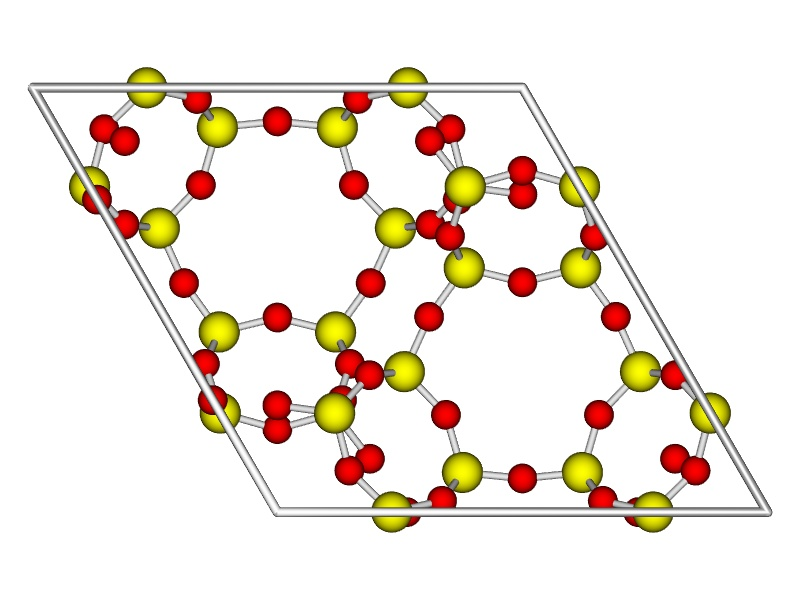
\includegraphics[width=7.5cm]{./Visualization/ERI_ball_stick_front.jpg}}
  \subfloat[]{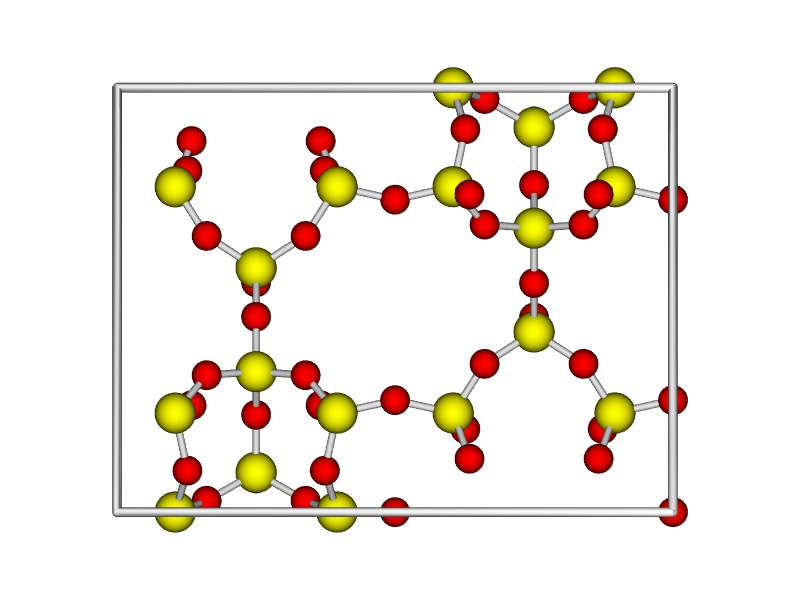
\includegraphics[width=7.5cm]{./Visualization/ERI_ball_stick_side.jpg}}
  \caption{Ball and stick picture of erionite (ERI): (a) front view, (b) side view. The erionite structure is
           monoclinic: $a=b=13.27$ \AA\ and $c=15.05$ \AA, $\alpha=\beta=90^\circ$ and $\gamma=120^\circ$.}
  \label{Fig: ERI ball-and-stick}
\end{figure}

After copying the vtk-files to `Examples/Visualization/ERI/VTK' one can run the VTK code. The VTK program
will produce a picture `Picture.jpg' and looks like Figure \ref{Fig: ERI ball-and-stick}.
The file `Frame.vtk' looks like:
\begin{verbatim}
     # vtk DataFile Version 1.0
     Frame
     ASCII

     DATASET POLYDATA
     POINTS 8 float
     50.000000 -0.000000 -0.000000
     150.000000 0.000000 0.000000
     100.000000 86.602540 0.000000
     0.000000 86.602540 0.000000
     50.000000 0.000000 113.413715
     150.000000 0.000000 113.413715
     100.000000 86.602540 113.413715
     0.000000 86.602540 113.413715
     LINES 6 36
     5 0 1 2 3 0
     5 4 5 6 7 4
     5 0 1 5 4 0
     5 2 3 7 6 2
     5 0 4 7 3 0
     5 1 2 6 5 1
\end{verbatim}
It contains 8 points: the corners of the frame, and 6 closed poly-lines that form the ribbons. Using the `vtkTubeFilter'
we can use these lines to turn them into bigger tubes and color the tubes white.
The coordinate system is chosen as $150\times150\times150$ to be compatible with structure grids (for the density and surface).
The information about the framework is listed in `FrameworkAtoms.vtk':
\begin{verbatim}
     # vtk DataFile Version 1.0
     Cube
     ASCII

     DATASET POLYDATA
     POINTS 108 float
     38.346000 20.221693 11.847197
     38.125000 36.762778 28.353429
     35.205000 30.250267 18.259608
     ....
     ....
     LINES 232 696
     2 0 2
     2 0 3
     2 0 13
     ....
     ....
     POINT_DATA 108
     SCALARS my_scalars float
     LOOKUP_TABLE default
     2.1
     2.1
     1.52
     ....
     ....
     VECTORS vectors float
     0.125 0 0
     0.125 0 0
     0.03125 0 0
     ....
     ....
\end{verbatim}
The first points are the 108 framework atoms, next the lines section describes the bonding between them.
The last two sections denote the size and color of the atoms (Note that the VECTORS section is a trick to
allow the VTK `glyphs', here spheres, to be scaled by the scalar data, but colored by the magnitude of the
VECTOR data. Hopefully this will be easier in future versions of VTK).

The VTK program is also interactive, one can zoom in and out (scroll button) and rotate (click on the canvas, closer
to the center rotates less then further away). In computer graphics, a sphere is not a sphere, but a collection
of polygons. More polygons means a smoother surface but less responsive in the interactive mode.
For final pictures, one should use many polygons and anti-aliasing, which really improve the quality of the
picture.

The VTK files are written in `src/movies.c' in the routine `void WriteVTK(int system)'. The top of this file also
defines the colors. This same color definition is also used in the VTK `main.c'.

\section{Framework surface}

The ball and stick pictures are useful, but still do not provide information about pore shape and connectivity.
A more suitable approach is to visualize the energy landscape for a certain probe atom.
For energy landscape pictures, we divide the unit cell
into e.g. $150\times150\times150$ voxels (volume-elements).
At millions of random positions in the unit cell
the free energy of a test-particle (usually a helium or methane unit atom) is calculated
and assigned to the appropriate voxel. To visualize this energy landscape
the three-dimensional dataset is volume rendered,
removing the parts that generate overlap (the structure itself) by making it
completely transparent.
Low energy values are rendered with medium transparency, allowing the inside of the pores/cages to
be viewed as voids. Higher energy values are rendered less and less
transparent until the energy approaches
a cutoff energy and is regarded as part of the zeolite wall. Also color is assigned according
to the energy value (green for the outside view of a cage).

To speed up computation of surface and density pictures it is advisable to use energy-grids. For the upcoming example
we need grids for CO$_2$-atoms and helium:

\begin{verbatim}
     SimulationType                   MakeGrid

     Forcefield                       ExampleZeolitesForceField

     Framework 0
     FrameworkName ERI_mono
     UnitCells 3 3 2
     ExternalTemperature 300.0

     NumberOfGrids 3
     GridTypes O_co2 C_co2 He
     SpacingVDWGrid 0.1
     SpacingCoulombGrid 0.1
\end{verbatim}
We need $3\times3\times2$ unit cells to obey the minimum-image convention.

Next we are going to generate the VTK `FrameworkatomsSurface.vtk' that contains data on the energy-grid for a chosen
probe atom. Here, we use helium.
An example input to generate the surface-grid is listed here (`Example/Visualization/ERI/SurfaceRASPA')
\begin{verbatim}
     SimulationType                   Visualization
     NumberOfCycles                   10000000000
     PrintEvery                       100000

     Forcefield                       ExampleZeolitesForceField
     ChargeMethod                     None

     Framework 0
     FrameworkName ERI_mono
     UnitCells 3 3 2
     ExternalTemperature 300.0

     NumberOfGrids 1
     GridTypes He
     SpacingVDWGrid 0.1
     SpacingCoulombGrid 0.1
     UseTabularGrid yes

     component 0 MoleculeName                     helium
                 MoleculeDefinition               ExampleDefinitions
                 IdealGasRosenbluthWeight         1.0
                 BlockPockets                     no
                 BlockPocketsFileName             ERI_mono
                 CreateNumberOfMolecules          0
\end{verbatim}

Even though the grid is generated for a single unit, in general one still needs $3\times3\times2$ unit cells because
the charge interaction is dependent on the amount of chosen unit cells.
The grid file `FrameworkSurface.vtk' is located in `VTK/System[int]'.

To visualize the pore-shape, copy the `FrameworkSurface.vtk' to `Examples/Visualization/ERI/VTK'. Do not copy the other VTK files
because they are generated for a $3\times3\times2$ grid, and we need the framework-atoms and frame- VTK files
for a $1\times1\times1$ structure.
Running the VTK-program now shows the surface inside the structure, as shown in
Figure \ref{Fig: ERI density}(a). If we compare Figure \ref{Fig: ERI density}(a) to Figure \ref{Fig: ERI ball-and-stick}
we see that we have visualized the pore structure itself. Also note, that small ``pockets'' have shown up that are not a
part of the main pore system. These pockets should be blocked (See next section).

The ERI-case by default offers a nice view inside the cage. This is not always the case. Using
\begin{verbatim}
     ShiftUnitCells 0.25 0 0 
\end{verbatim}
one can change the LTA case to a outside-cage-view to an inside-cage-view. (TODO, check whether grids takes this into account.)

\begin{figure}[t]
  \centering
  \subfloat[]{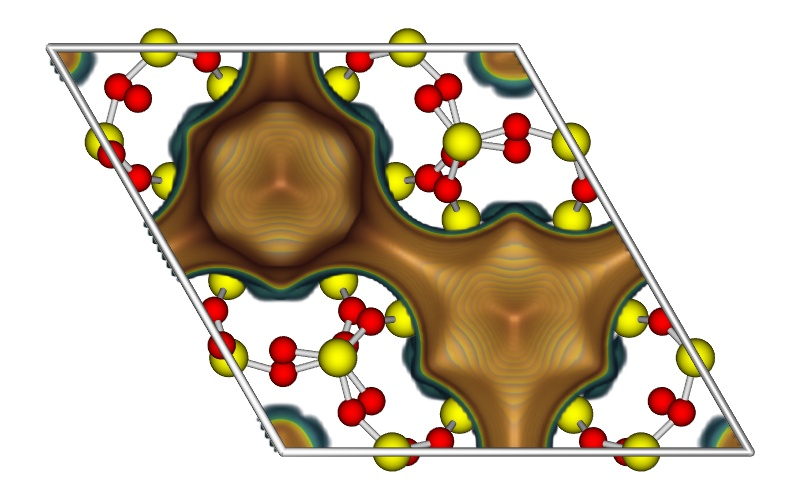
\includegraphics[width=7.5cm]{./Visualization/ERI_surface.jpg}}
  \subfloat[]{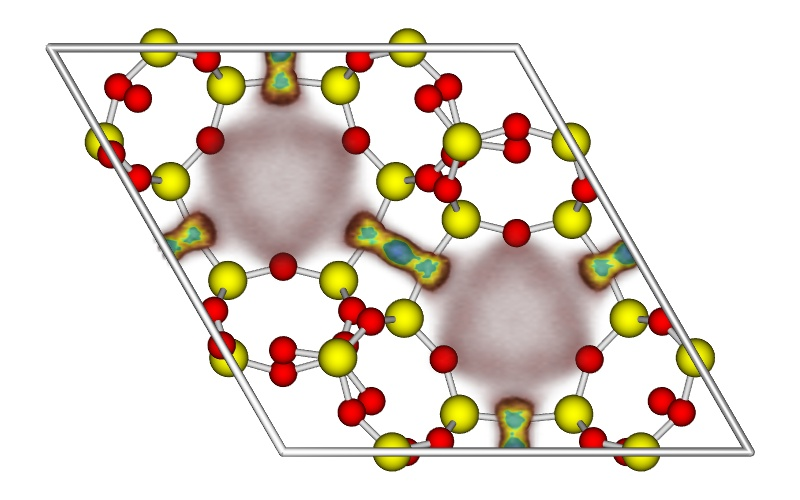
\includegraphics[width=7.5cm]{./Visualization/ERI_CO2_density.jpg}}
  \caption{Picture of ERI: (a) surface picture, (b) density picture (1 CO$_2$ at 300K).}
  \label{Fig: ERI density}
\end{figure}

The `FrameworkSurface.vtk' is a structured points VTK-file. It is rectangular grid of, in this case,
$150\times150\times150$ points (a total of 3375000 points). All these values are listed sequentially,
but one can convert between 1D and 3D by using 
\begin{equation}
\text{index}=x+y*\text{SIZEY}+z*\text{SIZEX}*\text{SIZEY}
\end{equation}
Note that the proper aspect ratios can be used. The VTK file looks like
\begin{verbatim}
     # vtk DataFile Version 1.0
     Free energy zeolite: ERI_mono (300.000000 K)
     ASCII
     DATASET STRUCTURED_POINTS
     DIMENSIONS 150 150 150
     ASPECT_RATIO 1.000000 0.577350 0.756091
     ORIGIN 0.0 0.0 0.0

     POINT_DATA 3375000
     SCALARS scalars unsigned_short
     LOOKUP_TABLE default
     0
     0
     ....
     ....
\end{verbatim}
The stored values are `unsigned short', so between 0 and 65536 ($2^{16}$). The value are always clipped to this region
using the minimum and maximum values of the simulation data.

\begin{figure}[t]
  \centering
  \hskip -0.5cm
  \subfloat[]{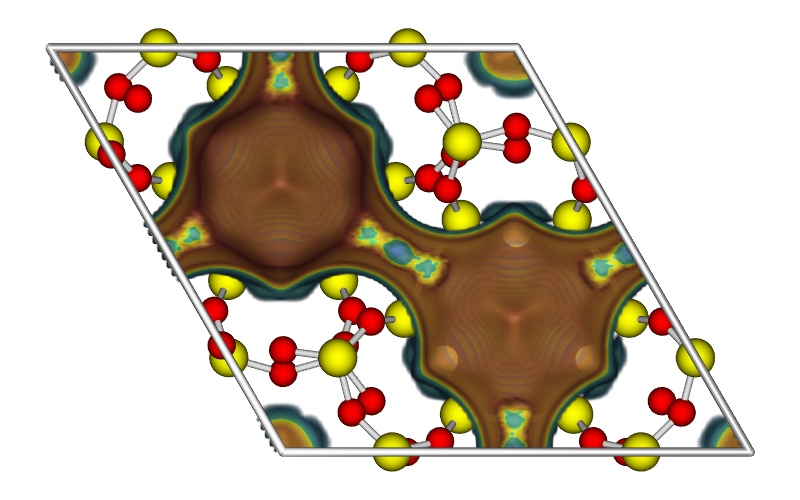
\includegraphics[width=7.5cm]{./Visualization/ERI_picture_all.jpg}}
  \hskip -0.5cm
  \subfloat[]{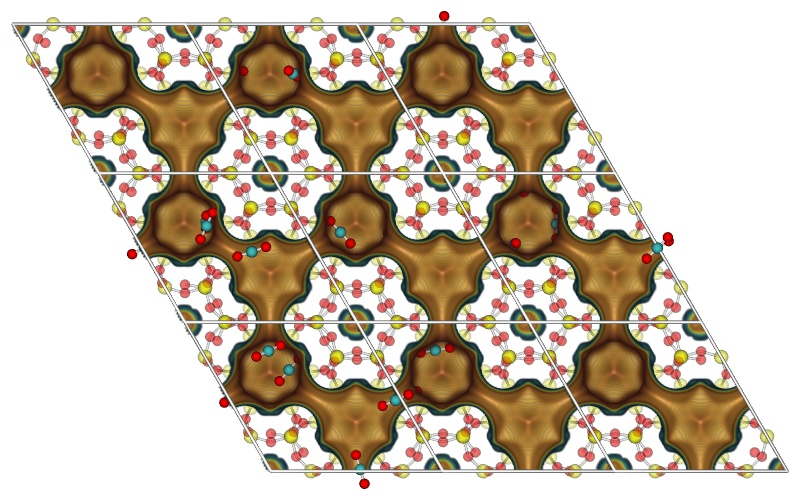
\includegraphics[width=9.75cm]{./Visualization/ERI_snapshot.jpg}}
  \caption{}
  \label{Fig: ERI picture all}
\end{figure}

\section{Density plots}

During a Monte Carlo simulation a 3-dimensional histogram of the positions
of all atoms of the molecules is collected (per component). The unit cell is divided into 150x150x150 "voxels".
During the simulation the molecules move around in the box, and every cycle data is collected
for the histogram. First a position is mapped back from the full simulation box (3x3x2 unit cells)
to the main unit cell, and for every atom the voxel corresponding to the mapped position is incremented.
At certain intervals the histogram is written to file so that it can be visualized using VTK.
The data is always normalized using the highest occurring voxel value. However, the overall brightness
is still influenced by the loading of the specific adsorbate in the mixture.

In VTK the data is "volume rendered", more dense regions are less transparent, less dense regions are
more transparent. In addition the color changes, less dense regions are grey, more dense are orange,
then yellow, and the highest is rendered light blue. The original framework is placed in the picture as
a ball-and-stick model, and every position can be related to the framework.
We can therefore e.g. decipher a molecular picture of why selectivity occurs.

An example input for RASPA is
\begin{verbatim}
     SimulationType                   MC
     NumberOfCycles                   100000000
     NumberOfInitializationCycles     100
     PrintEvery                       100
     PrintPropertiesEvery             10000

     Forcefield                       ExampleZeolitesForceField

     Framework 0
     FrameworkName ERI_mono
     UnitCells 3 3 2
     ExternalTemperature 300.0
     ComputeDensityProfile3DVTKGrid   yes
     WriteDensityProfile3DVTKGridEvery 10000
     DensityProfile3DVTKGridPoints 150 150 150

     NumberOfGrids 2
     GridTypes C_co2 O_co2
     SpacingVDWGrid 0.1
     SpacingCoulombGrid 0.1
     UseTabularGrid yes

     component 0 MoleculeName                     CO2
                 MoleculeDefinition               ExampleDefinitions
                 IdealGasRosenbluthWeight         1.0
                 TranslationProbability           1.0
                 RegrowProbability                1.0
                 SwapProbability                  0.0
                 CreateNumberOfMolecules          1
\end{verbatim}

Copy the `VTK/System[int]/DensityProfile\_methane.vtk' to `Examples/Visualization/ERI/VTK' as `Density.vtk',
rename the surface VTK-file,
and run the vtk-code. It will now produce a picture like Figure \ref{Fig: ERI density}(b).
If you did not rename the file (or rename it again to `FrameworkatomsSurface.vtk'), a picture with the frameworks atoms,
the pore surface and the density of CO$_2$ is produced. It is now easy to show that CO$_2$ preferentially adsorbs
in the 8-ring windows separating the erionite cages (in contrast to an alkane which prefers the cages).

Of course, one is not restricted to a unit cell and it is possible to make pictures of bigger volumes.
The first way is to use $3\times3\times2$ unit cells, and use the file `Movies/System[int]/Framework\_initial.cssr'.
Copy this file as `structure\_name\_3x3x2.cssr' and from then on use $1\times1\times1$ using this new enlarged unit cell.
The second method is to use $3\times3\times2$ unit cell but copy the surface and density in the $x$, $y$, $z$ directions
in the picture. You have to edit the `main.c' file of the VTK directory and recompile. The relevant settings are:
\begin{verbatim}
     // the resolution of spheres and tubes, the higher the more smooth
     // use 10, but 50 for the final picture
     const int Resolution=10;

     // anti-aliasing, use 1, but 16 for final picture
     const int AA=1;

     // control the transparancy of framework, adsorbates, and cations
     const double FrameworkOpacity=1.0;
     const double AdsorbateOpacity=1.0;
     const double CationOpacity=1.0;

     // zoom in or out by increasing/decreasing the zoom-factor
     const double ZoomFactor=2.0;

     // scale the size of the atoms and bonds
     const double ScaleFactor=1.0;

     // control the view-point of the oject (input in degrees)
     const double Azimuth=0.0;
     const double Elevation=0.0;
     const double Roll=0.0;

     // the size of the image in pixels
     const int ImageSizeX=800;
     const int ImageSizeY=500;

     // the number of duplicates in x,y,z (same as the number of unit cells)
     const int NrDuplicatesX=3;
     const int NrDuplicatesY=3;
     const int NrDuplicatesZ=2;

     // the lengths of the edge-vectors
     const double A=13.27;
     const double B=13.27;
     const double C=15.05;

     // the angles of the unit cell
     const double AlphaAngle=90*M_PI/180.0;
     const double BetaAngle=90*M_PI/180.0;
     const double GammaAngle=120*M_PI/180.0;
\end{verbatim}
This can then be used to make a `snapshot' of molecules. For the $3\times3\times2$ structure we need the file
`VTK/System[int]/AdsorbateAtoms.vtk' from a simulation. This file is generated at the start of a simulation. 
After a sufficiently long run to equilibrate the molecules, one
could copy the `Restart' to `RestartInitial', put the amount of created molecules at zero and restart from the
restart-files using zero cycles to generate the new `AdsorbateAtoms.vtk' file.
The picture of a snapshot of 64 CO$_2$ in the $3\times3\times2$ ERI-structure is shown in
Figure \ref{Fig: ERI picture all}(b). Note the many CO$_2$ molecules that occupy the barrier. Conclusions
are hard to draw based on snapshots. The `density'-plots give average information and therefore the same for
each unit cell (because each unit cell is the same [using a rigid structure]). The density plots are based on
atoms, and one can clearly see the orientation of CO$_2$ on the barrier. The 3 `blobs' corresponds to the oxygen, carbon,
and oxygen of CO$_2$.

\begin{figure}[t]
  \centering
  \subfloat[]{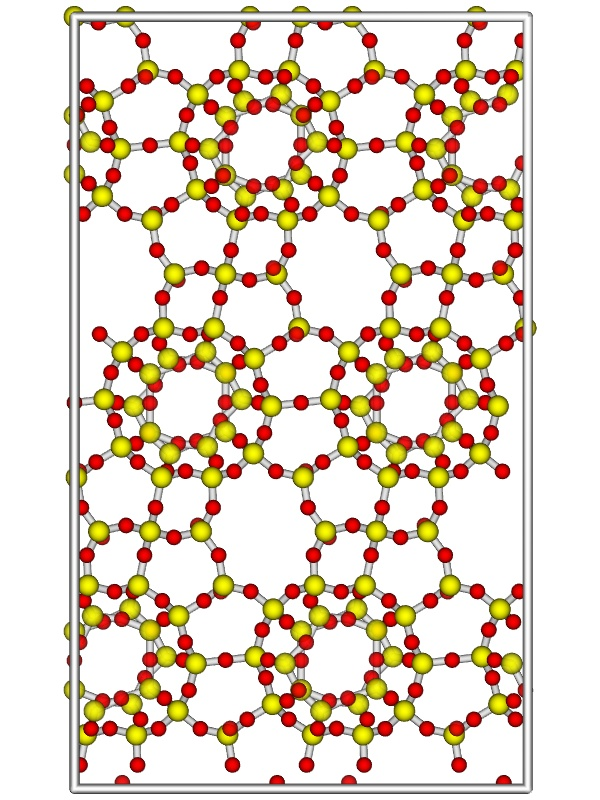
\includegraphics[width=5.0cm]{./Visualization/DDR_picture_1.jpg}}
  \subfloat[]{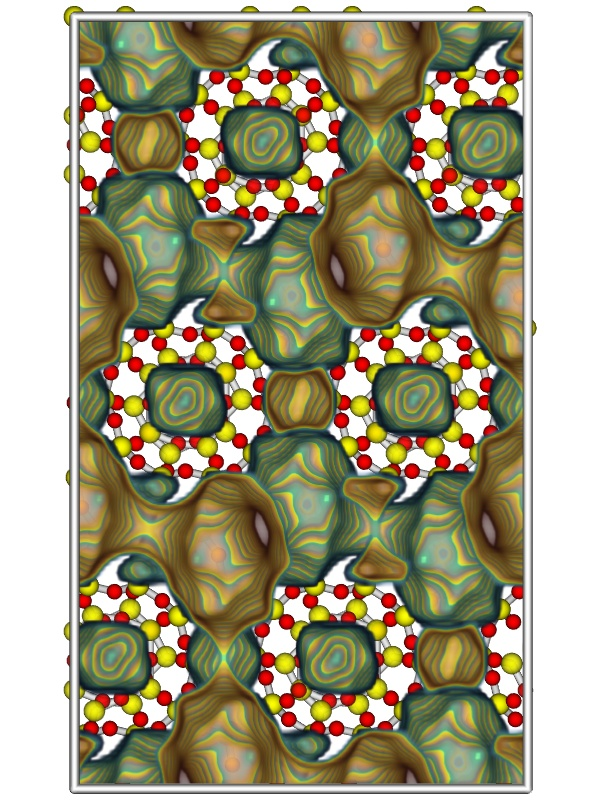
\includegraphics[width=5.0cm]{./Visualization/DDR_picture_2.jpg}}
  \subfloat[]{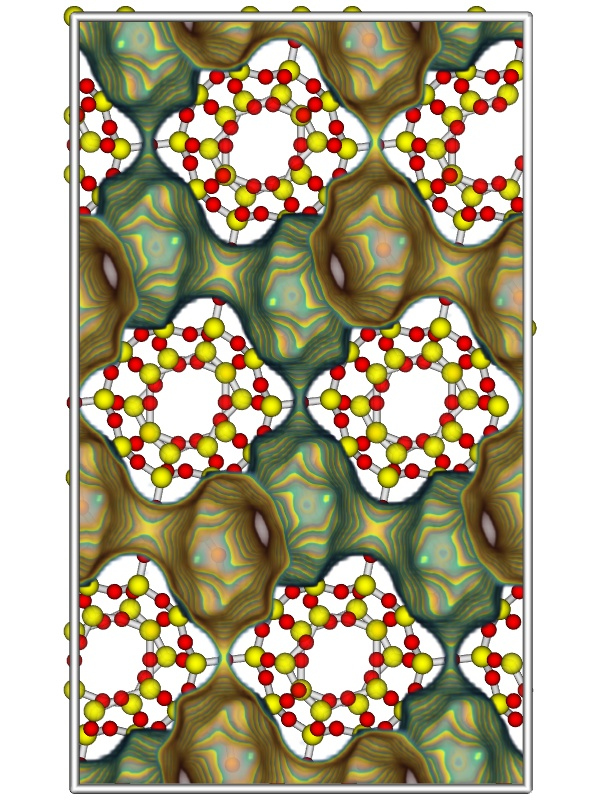
\includegraphics[width=5.0cm]{./Visualization/DDR_picture_3.jpg}}
  \caption{Blocking pockets in DDR. The DDR structure is converted to a orthorhombic unit cell of
   $a=24.006,b=13.86$, and $c=40.892$ \AA. In (a) we show the ball-and-stick structure, in (b) the structure
   and the pore surface probed with helium, and (c) the structure with proper blocking of the small disconnected pockets.}
  \label{Fig: DDR blocking}
\end{figure}

\section{Determining blocking pockets}

Some structures have inaccessible parts, i.e. areas that are not reachable from the main pore system. Examples
are the sodalite cages in FAU- and LTA-type zeolites. The surface pictures allow us to visualize these pockets,
locate the position, and construct a `blocking-file'.

The unit cell of the DDR structure has edge lengths of a=24.006 Angstrom, b=13.86 Angstrom, 40.892 Angstrom 
with cell angles of 90 degrees. The atomic structure is shown in Figure \ref{Fig: DDR blocking}(a). It is difficult to envision 
the details of the pore structure from this picture. One can obtain more insight from energy-landscapes.
In Figure \ref{Fig: DDR blocking}(b) we show the same structure with the energy landscape a helium atom would feel. In practice, 
the simulation cell is divided into 150x150x150 bins and during a Monte-Carlo simulation one keeps track of 
the average energy a molecule feels inside that bin. Here we volume-rendered the resulting energy grid 
making very high energies transparent, i.e. the part that overlaps with the framework, as well as very 
favorable energies, i.e. the positions inside the cage. The resulting surface layer can be viewed as the 
"wall" of the pores. Alternatively, one can make a isocontour (a surface representing a constant, 
high value of the energy). In Figure \ref{Fig: DDR blocking}(b) the main pore structure is apparent, 
but also some disconnect pockets show up. It is 
very important to artificially block these pockets for Monte-Carlo simulations. Also, in 
Molecular Dynamic simulations, initial positions should be chosen in the main channel system. The blocking 
procedure can be a simple distance-check from the center of the small pockets and a rejection of all 
Monte-Carlo trial moves that would place a molecule inside a certain radius. This radius should not be 
chosen to small or too big, because otherwise one would block not enough, or block parts of the 
main channel system. In Figure \ref{Fig: DDR blocking}(c) we show the structure with the appropriate blocking centers and radii; 
all small pockets have disappeared but the main channel system is unchanged.

The blocking procedure is dependent on the type of probe atom. Helium is a good procedure to find small pockets 
and therefore to obtain the proper unit cell pore volume. This accessible pore volume is in simulation 
usually obtained via a helium-probe procedure. Helium can also be used to find pockets that 
could be occupied by other small molecule like CO2, N2, H2, methane, etc.
The adsorption results can be dramatically different with or without blocking. Whether the selectivity of 
mixtures changes to higher or lower depends on the match of the molecule with the small pockets. 
The small pockets are very favorable for the small molecules because they tend to have a very surface high 
curvature, i.e.. a very favorable interaction energy). 

\section{Making movies}

\subsection{Using VMD}

\subsection{Combining pictures into a movie}

Using ``ffmpeg'', from png-files to a mov-file with h264-encoding
\begin{verbatim}
ffmpeg -i %03d.png -s:v 1280x720  -acodec aac -ac 2 -strict experimental -ab 160k 
-vcodec libx264 -preset slow -profile:v baseline -level 30 -maxrate 10000000 
-bufsize 10000000 -b 1200k -f mp4 -threads 0  -crf 23 -pix_fmt yuv420p -r 30 Movie.mov 
\end{verbatim}
or using ``mencoder'' with settings 
\begin{footnotesize}
\begin{verbatim}
export opt="vbitrate=1280000:mbd=2:keyint=132:vqblur=1.0:cmp=2:subcmp=2:dia=2:mv0:last_pred=3"
mencoder -ovc lavc -lavcopts vcodec=msmpeg4v2:vpass=1:$opt -mf type=jpg:fps=25 -nosound -o /dev/null mf://\*.jpg
mencoder -ovc lavc -lavcopts vcodec=msmpeg4v2:vpass=2:$opt -mf type=jpg:fps=25 -nosound -o output.avi mf://\*.jpg
\end{verbatim}
\end{footnotesize}



\chapter*{Appendix}

\section*{Random numbers}

\subsection*{32-bits version}
\begin{verbatim}
     A C-program for MT19937, with initialization improved 2002/1/26.
     Coded by Takuji Nishimura and Makoto Matsumoto.

     Before using, initialize the state by using init_genrand(seed)  

     Copyright (C) 1997 - 2002, Makoto Matsumoto and Takuji Nishimura,
     All rights reserved.                          

     Redistribution and use in source and binary forms, with or without
     modification, are permitted provided that the following conditions
     are met:

       1. Redistributions of source code must retain the above copyright
          notice, this list of conditions and the following disclaimer.

       2. Redistributions in binary form must reproduce the above copyright
          notice, this list of conditions and the following disclaimer in the
          documentation and/or other materials provided with the distribution.

       3. The names of its contributors may not be used to endorse or promote 
          products derived from this software without specific prior written 
          permission.

     THIS SOFTWARE IS PROVIDED BY THE COPYRIGHT HOLDERS AND CONTRIBUTORS
     "AS IS" AND ANY EXPRESS OR IMPLIED WARRANTIES, INCLUDING, BUT NOT
     LIMITED TO, THE IMPLIED WARRANTIES OF MERCHANTABILITY AND FITNESS FOR
     A PARTICULAR PURPOSE ARE DISCLAIMED.  IN NO EVENT SHALL THE COPYRIGHT OWNER OR
     CONTRIBUTORS BE LIABLE FOR ANY DIRECT, INDIRECT, INCIDENTAL, SPECIAL,
     EXEMPLARY, OR CONSEQUENTIAL DAMAGES (INCLUDING, BUT NOT LIMITED TO,
     PROCUREMENT OF SUBSTITUTE GOODS OR SERVICES; LOSS OF USE, DATA, OR
     PROFITS; OR BUSINESS INTERRUPTION) HOWEVER CAUSED AND ON ANY THEORY OF
     LIABILITY, WHETHER IN CONTRACT, STRICT LIABILITY, OR TORT (INCLUDING
     NEGLIGENCE OR OTHERWISE) ARISING IN ANY WAY OUT OF THE USE OF THIS
     SOFTWARE, EVEN IF ADVISED OF THE POSSIBILITY OF SUCH DAMAGE.
\end{verbatim}

\subsection*{64-bits version}
\begin{verbatim}
     A C-program for MT19937-64 (2004/9/29 version).
     Coded by Takuji Nishimura and Makoto Matsumoto.

     This is a 64-bit version of Mersenne Twister pseudorandom number
     generator.

     Before using, initialize the state by using init_genrand64(seed)  

     Copyright (C) 2004, Makoto Matsumoto and Takuji Nishimura,
     All rights reserved.                          

     Redistribution and use in source and binary forms, with or without
     modification, are permitted provided that the following conditions
     are met:

       1. Redistributions of source code must retain the above copyright
          notice, this list of conditions and the following disclaimer.

       2. Redistributions in binary form must reproduce the above copyright
          notice, this list of conditions and the following disclaimer in the
        documentation and/or other materials provided with the distribution.

       3. The names of its contributors may not be used to endorse or promote 
          products derived from this software without specific prior written 
          permission.

     THIS SOFTWARE IS PROVIDED BY THE COPYRIGHT HOLDERS AND CONTRIBUTORS
     "AS IS" AND ANY EXPRESS OR IMPLIED WARRANTIES, INCLUDING, BUT NOT
     LIMITED TO, THE IMPLIED WARRANTIES OF MERCHANTABILITY AND FITNESS FOR
     A PARTICULAR PURPOSE ARE DISCLAIMED.  IN NO EVENT SHALL THE COPYRIGHT OWNER OR
     CONTRIBUTORS BE LIABLE FOR ANY DIRECT, INDIRECT, INCIDENTAL, SPECIAL,
     EXEMPLARY, OR CONSEQUENTIAL DAMAGES (INCLUDING, BUT NOT LIMITED TO,
     PROCUREMENT OF SUBSTITUTE GOODS OR SERVICES; LOSS OF USE, DATA, OR
     PROFITS; OR BUSINESS INTERRUPTION) HOWEVER CAUSED AND ON ANY THEORY OF
     LIABILITY, WHETHER IN CONTRACT, STRICT LIABILITY, OR TORT (INCLUDING
     NEGLIGENCE OR OTHERWISE) ARISING IN ANY WAY OUT OF THE USE OF THIS
     SOFTWARE, EVEN IF ADVISED OF THE POSSIBILITY OF SUCH DAMAGE.

     References:
     T. Nishimura, ``Tables of 64-bit Mersenne Twisters''
       ACM Transactions on Modeling and 
       Computer Simulation 10. (2000) 348--357.
     M. Matsumoto and T. Nishimura,
       ``Mersenne Twister: a 623-dimensionally equidistributed
         uniform pseudorandom number generator''
       ACM Transactions on Modeling and 
       Computer Simulation 8. (Jan. 1998) 3--30.
\end{verbatim}



\section*{Acknowledgements}
We would like to thank the following people for their help and input to improve the program and for
the very helpful discussions about the algorithms: Sayee Prasaad Balaji, Youn-Sang Bae, Xiaoying Bao, Roc\'io Bueno P\'erez,
Nicholas C. Burtch, Tom Caremans, Ana Mart\'in Calvo, Yamil Colon,
Juan Manuel Castillo Sanchez, Allison Dickey, Tina D\"uren, Titus van Erp, Denise Ford,
Houston Frost, Rachel Getman,  Pritha Ghosh, Elena Garc\'ia P\'erez, Gloria Oxford, Sudeep Punnathanam, Almudena Garcia Sanchez, Juan Jose Gutierrez Sevillano,
John J. Low, Patrick Merkling, Patrick Ryan, Lev Sarkisov, Ben Sikora, Ariana Torres Knoop, Krista S.\ Walton, Chris Wilmer, Ozgur Yazaydin, and Decai Yu.
Very special thanks to Thijs Vlugt.

\end{document}
